\documentclass[a4paper,twocolumn,11pt,unpublished]{quantumarticle}
\pdfoutput=1
\pdfinfoomitdate=1
\pdftrailerid{}
\pdfsuppressptexinfo=15

\usepackage[utf8]{inputenc}
\usepackage[english]{babel}
\usepackage[T1]{fontenc}
\usepackage{amsmath,amssymb}
\usepackage{amsthm}
\usepackage{booktabs}
\usepackage{graphicx}
\usepackage{placeins}
\usepackage{float}
\usepackage{needspace}
\usepackage{microtype}
\usepackage[numbers]{natbib}
\usepackage{hyperref}
\usepackage{orcidlink}

% The class loads Latin Modern at begin-document time.  Re-select the document
% font immediately afterwards so no bitmap EC fonts leak into the PDF.
\AtBeginDocument{\normalfont}

% Preserve the honest unpublished status while using Quantum's traditional
% violet presentation for the title, hyperlinks, and page numbers.
\hypersetup{allcolors=quantumviolet}
\makeatletter
\renewcommand{\@printtitle}{%
  \color{quantumviolet}%
  \@printtitletextwithappropriatefontsize\par\vspace{0.25em}%
  
}
% The class stores each ORCID and links the author name.  Also display the
% standard green ORCID mark, as in published Quantum articles.
\def\@printauthor#1#2{%
  \def\footnote{\ClassError{quantumarticle}{You must not put a
  \string\footnote{} command inside the argument of \string\author}{}}%
  \mbox{%
    \ifcsdef{author#1orcid}{%
      \href{https://orcid.org/\csname author#1orcid\endcsname}%
        {\color{black}#2}\,\orcidlink{\csname author#1orcid\endcsname}%
    }{#2}%
  }%
  \ifnumcomp{\the@affiliationcounter}{>}{1}{%
    \textsuperscript{\forlistcsloop{\@@commaspacebefore}%
      {author#1affiliations}\unskip}%
  }{}%
  \ifnumcomp{#1}{<}{\the@authorcounter-1}{, }{%
    \ifnumcomp{#1}{=}{\the@authorcounter-1}{%
      \ifnumcomp{#1}{=}{1}{ and~}{, and~}%
    }{}%
  }%
}
% Identify authors with contact details as corresponding authors and repeat
% their linked ORCID mark in the contact line.
\def\@printauthorextrainfo#1{%
  \vspace{0.55\baselineskip}%
  \raggedright
  \textit{Corresponding author}\par
  \csname @authorname#1\endcsname
  \ifcsdef{author#1orcid}{%
    \,\orcidlink{\csname author#1orcid\endcsname}%
  }{}\enspace
  \ifcsdef{author#1emails}{%
    \forlistcsloop{\@@spaceafter}{author#1emails}%
  }{}%
  \ifcsdef{author#1homepages}{%
    \ifcsdef{author#1emails}{\unskip, }{}%
    \forlistcsloop{\@@spaceafter}{author#1homepages}%
  }{}%
  \ifcsdef{author#1thanks}{%
    \ifcsdef{author#1emails}{%
      \ifcsdef{author#1homepages}{\unskip, }{\unskip, }%
    }{%
      \ifcsdef{author#1homepages}{\unskip, }{}%
    }%
    \forlistcsloop{\@@spaceafter}{author#1thanks}%
  }{}%
  \par\vspace{-0.55\baselineskip}%
}
\fancyfoot[C]{\sffamily\textcolor{quantumviolet}{\thepage}}
\makeatother

\newtheorem{theorem}{Theorem}
\newcommand{\D}{\mathcal{D}}
\newcommand{\Tr}{\operatorname{Tr}}

\renewcommand{\dbltopfraction}{0.95}
\renewcommand{\dblfloatpagefraction}{0.5}
\setcounter{dbltopnumber}{2}
\setcounter{totalnumber}{6}
\setcounter{topnumber}{4}
\renewcommand{\topfraction}{0.9}
\renewcommand{\textfraction}{0.05}
\renewcommand{\floatpagefraction}{0.5}

\hypersetup{pdftitle={Stronger dissipation, longer memory: engineering the jump operators of quantum reservoirs},
 pdfsubject={Dissipation engineering, dark states and the memory of quantum reservoirs}}
\begin{document}
% Data-only certificate archive, encoded as a PDF ASCIIHex stream.
\begingroup
\pdfcompresslevel=0
\immediate\pdfobj stream attr {
  /Type /EmbeddedFile /Filter /ASCIIHexDecode
  /Params << /Size 107007 >>
} {
504b030414000000080000002100ea7a4331de020000400500000a000000524541444d452e7478746d54cb8e1b3710bc
cf57f4076846487cf36d113b80010736bc7bc84d68912d0dbd1c926e925a4dbe3e45cecaab200604bdc8eeaeaec73c26
17c888167772868b90e194ab173a45a527595254f614d58a523cd1224bd4955093341631452cfda81c4a5d48258b5ea2
d33c0c4fb3cb9417f69e129b673e0b5d44314332951953a2f7a87617197dccb8da60b8900b072379774384ee26d6e45d
380f41dc793e469d63b4b8b17509c5851a6ba6858b99c58e56d1130772c23e4e4241d70258ec77c4c1b6b2e1e4822b32
6a5f37cea282a1aff750e16298e85321f639e25fe3ab7d451dea82250cfbe154bd1f174e84a1e6b931d3ceb324ee5d39
b05f8b33f857052bca453c2dd18a6f9dd1ec25be3503a965c64e54b3d0831e871be2dc11bb602509de42f12bc9b528a7
e8b931df50100eb22b2bd0147557109172876f2350875806951fd5a974849ef50c250be7e73d1a7d87064d4f563383b7
89fed4b8e022c4b328d90e634053f3e571ff195c5fdf0f03515a8138bc9b7e7b47e30265c385a626198efae7fee8c27e
bbd42e249736710177d47bbb8dafe0166c97a772fd6587ee9cf5705796a7b4d28862232e959bb5ecf43dc700f345d21a
fabe77e47581dbf25fb97a37b23fcb51b9532c5736851e4bd565cc096b2becdc951d361afcbaebeafc0f9a5c9c6deed9
2bbec9cb81ab7565dffb1d5c48b534a4a015616acebb87f3a6ffbd49fad41d9c246fbdcf12042984c807c8dfe48e61ff
ede3c387bf3e36caa661f826a75717ab24cf6b036be98faf1bc8a6d3f4fb440fb08322939d9d175766e29c1ba9316492
c0478fa2a5e6322405599dc053ac8a08e78c08be05f416a55becfe13b8be023cd89f012e0f4c3eb6354d5c4008b771f8
b56966788bdbd37c171a3c5a10a8ee7d64655e53c4a82c194e5eb83f27faecc449145bc1546c41fbd637976a57b25c20
ad3603d0268de801603114b99afe716937f0859d6f4bffcc2df2d5a672db0f2fe33cf2b2d2c979b90d7d92bf29d7e3e2
7253611afe05504b03041400000008000000210012b1ef0d460900005f1300000e00000053484132353653554d532e74
78748d984b729cc71184f73c052f60b1df8fa523aca537be00a2bbba8a1c0b9c81060399bcbdbf0620696003a0360870
02f3e75f55599959345f570a794537525ec366965c7bf25997e669c1f2707dd654a40f1da673399d75c4912ce88ce9e3
c77ffdfcf77ffcf3e79f2edf2e1f8a4fe6564ad3cd1272f6a5caaa25375ffd6cb1bbd047cdae75f57efa38ad3a7e8dde
2fdf55d5af8f1f45cf97831d645cf46f67fdf5e170d6af7abcdc3f3ebe59a95383cdd49b685cb9069fc66852ba0469ae
698f7e4a59219429b3f8e5ba1b2bda108b4de6c78ffadb61e951f4d33c1fd667fd740577ffd3bfef4fc70fc1b951ace5
a1a9fa6c3de62a69a6914668a5e808a3cb68b125fe8c1e550bc5490c339b699c51dec2f8fed3ddf70fc9e98aa54d4d6a
2b46b7a66f6d040326aaa6e8b21f7ea5d65b4b41e8a38c511aef5f5a0549df7cf8cdd771912fba3648994325d2e99662
359ad446f7436df8c428d61a2586eec5cc8de6420ac51757631763ce32f32b20570fb7d9a3f610535cde5b34f3cd174b
0cba544b5198a4ad4015355156acda520dcd0fe76a2e515f19c1f3c36ffe7f144d7a0bce7bfa1e3d94eccda5d25748ea
293089f3f48ebec7c00418479f1176cc15aacb6e86f036d6ede1ebe1f204526bcb2de6242b3b49325d9669b3b6d69342
cf31576d34aa59a654de474a4c2ac640bc8b25bf32effbbbc3f1e6e9f7c78ee56ea9e5d5a76eca38ad99c2a68e1e6a65
eab9ec894baa2b6bd766754613e8354d8496b52b80ab16dd9cf954fff3c90ec7c3fe171f6d30a15b4ec46568bba2b058
2a5d720f0388b029e1636e4582495c3a6283c1233a7a905b483ebd0ff69b9e9f89ecf84e985ae76a7595ee197d6e9afc
b06ab25b28a6cdb9a2ae307f96db9511960cb61cd8e1af714e5ff4bc7fbb91d3f1723edd7eba1214b6ce07cf37d8ea5e
6962129468b13d09ad89c6c834ba5e72d491d2aacaf21b42e3e03a4b5adfc599e3f696d2440f77cf6468080ab4da4839
65af7e2e2bd928b20fd77ccf512a24703957f88c288652ba4325c66c9467efc2c13cf9e56683de3ff2a2f4ec139b3872
d552c42132daeb5a41a4a956df91b8987c80212bb2b0326bde8a071983367d17ebee7cba9ce474fb54962d175808163c
86b6661f710ab3e2993e88fa9067caad417349a34c5797d618d7f269029d6af96b50f75fd8c6f24166ccfb29881a8b3f
bb93e0860f1d3b68c34a1a0ead09c3c11d9c60f484f284b02ae43095d1df053bebfdc3ede5591f64b695bd5971d07c32
1e4b1dfd9938822b1e9f89c1cf590aabd4f73ed5e6ad853032432dabfd00e9e1f84874de6a8ea2bdb7e81cfb583d86b5
58df5cfac81ee5ac09f166aff3128c54113df8a2d842f1f57a7bd7f87a87f6fcfa300f9727323c6e6c63007df8814546
bc75b0fed133718f27d7ba495282c61a6aaf21a017088fc41873a82540bcb7004ee7a5e7cd6ef8f6d4aede57f1ce454b
2eaaab356574748582a7f32fbf6c4c4c691b3da4d6ed512131b86213e5b2fad790a8088f49ea9213a7b86fa7fd9b45a3
f8c89f289900aef1fca5abf7b1440b9484e4bc52649a723d96cf7ad4f3b83d5cbedfe8b78b1eef0fa7e3b53c38de4caa
1b33d3292ac833f07b4a865d283f6102abcb12a3bac1b5bd066daeaed870f556c68fa09e56f6767c9d6becd2340edfa4
95c5a8911b6245436025b140682d1ada37bb47edd433636b93f4814c90889cb459e28ff09e906e7ee3f3352e7cf234b9
085f151b6c54eb71f580a98a9acf959df22dc042fcb59a4f2e2cebde234ad6859894ebd017933beae1f397793a7f399d
d68d1dbee9baeea7f46c33fa4d10d6679a9f5573d7827d678f842c5f43c650ac354c7f79f6b8cf54526c4e9b0cf73ed0
ef59659ebee9a30476dc21cdb9486a9d399111078a3ef1f13d2ca1dec98bd8742a6d9189481726982689cf0864eb7db8
17cace663624101ec764683902d78318216244124527a5e2998a41057228e9cb080089ea6b9442847c0bea39515c3771
ecd0cbe81de590933a8d2bbc3496b8ed5c3753438c83243b1b13d25de81869e2fd4396b51f41bda88b840b19bb31a4d8
90295415c59e1a69574c6c1f8689197a253815c2067f89f4861cbcede85aff2218d37fa62236a1c3e7b4642b121169ad
3ca8728731167f11c7cc130e331bd87a352d52098d9dc0c4aeffb0b83f2386ef51e2280cc695686ba97674cf31371c53
fc4c1631177e10ca7bb7e87c150c8d944c3a5d769dfeceba1e64afd3cde342bf1816138f3df2922d93fd1a2322a4490b
15e5ab2d8039093518b163d3b77bfa5ad0290f6420cabc83f2a7c433eea646777c4227a692c133cbe3092f8b701194d8
1d6514419bbcf78924e898642048731ed83b184f7ef87cb9a0d831d66271185aceaae81ad36d6297c0bcba2f5ba6c47a
1d73e22e91db2e512b6991edf5efc03c4e6547c1fdd1f1b413fa6e1e374581c46354e27725f89752a3753cab66230504
cf52b7dea97d34bf944066f03cd5ed3318f10bc49d306fc6c3c251aee6b3025fee3e8701d61652c68df7e2819c16dd0c
1e4f081838d8322653ad52241a489cc6c666780b42bf0db9dc1c8e770fbfa709a2898b9340bc45ce058a0aab45560b29
25da755d24415114a32d6e4046d716671a640f58f48ba8f936126c40aac3e009647f541455976dc0c952406f5a5aab73
16735811abf119dc7239aecd9d5a0a79315f6bec3d967b387e7e11d55f263f7202274d8a4a5a769975119a43422350f2
1e8de8b702a389c654b8c8117c4e441aebb85a5ac9e54db0ef00317eb99cce8f55cd3916a49a5a588b9e3b21c9a1e543
508a8ca00f68d0b18d9ccbe329b29228e748cb92f9529caf0191c40ec787d3c32300954cbe40d3a627d5cdc57d6fc4b1
b83d61654bdebb3237cfb80607117edf9f2c30996f0c89f95d80ffe9da4c3caa843a1c8ae94323c7cc1ec8c37eb72d0f
75a4a25ca605b26ed97fc569eb3b1435d441fb2b5827b3cf9c84377f8882e38cc49a716aa8161c7ec0467095c100a264
c24cb97d773b177e5fcc91389cdbe1cc4202bbbe82f1c7445eb9a5f77f966cf9742b43572e34a4c513d356e0d8c1ea26
deba06539fdc70917d0ddb6c474bba334cf2afc25df78c68d9c9b2d801cd5e3108c1b808df268e233be44b9d33720d72
5123a6c161b600013853f4feb57a9ebce0c6c6d7c3eda32570134d442ccb0e599a52c366719e35b98dd0cd09192aa101
9dd8177da5634d1c1427fe41ee787dddee239d3dbdbb1d8f4f265ea4dd6d04ab22f95ce8c969903087eb01c7c1b21757
46b38d81dc990f21702749d99e9e9099e7977dd1791efc5f504b03041400000008000000210027ce518f2e0000002f00
00001c00000063657274696669636174652d726571756972656d656e74732e747874cb2bcd2da8b4b535d233d633e62a
4ece04710cf50ccdf48cb80a2a4b32f2f374d37232f34a6c6d0df42cf50cb800504b030414000000080000002100e313
1716ad0300005f0c00002100000065766964656e63652f6272696467652f6365727469666963617465732e6a736f6ebd
96ed4e5b490c86ff731551fe36393bfe1c7bafa452858ea01cba474b094ac2a2aaeabdef3b87a464294154e936480866
628fc77e1f7bbe9ecd66f3bb2fdbbf56b7fdf5cd78bb9dff399b972ebb325f4c5bebe1e3b819b17b396e37d8a4e46903
ebabf5555bf9807f67b3afd36f6c6c86e10aabe1d5a4e462bffc71757f07ff9f36fdc5a6c739c3a761ddaf2fb6e3eac9
47fb3cfd359b2da964d11a6a8582d36c71b08945b14ce72ab568faf7adf3c58bce3884c389a89014a5937c91929b8910
6991c84357e69c9a69a24c42fce4e9ec99c7f9f5b8de6cfbcfabcfc3edb6d792dedfad1e9094ebf5ea72b81def5b5ee6
1fa8d30c2f08be4af1ea245c226d58faecdd1fcb9974458725c7f9fcbbdf4bd465580f57fdf6615cdff41b24fdfee662
dddf34ef93cfd2958274aa292e1b5a27cfc58ac7ce27057cda81cf87f5b8859fc788b8237731524de48d1d4995dc8763
cd940e4cffbeb8bbbb980cb57318d5109c68aa61c212357786de0cf9c0f0aaec83b5244352a328a37224569a2426bbec
aa3d8bf572d83e9e57a373f6e2546b2d35ac5acb639dece8c740df53ff0fa47e39de8cdb2fbba371d11f3f7517b1b4cc
cbf97c72f06df12206caede7340a9823a0db94ccaa29a708772966a8342a9752026a3ac919541e85c543995deaa12f66
a39a19845d638d9339b0cea09e6241ce6450404493dfb0dcd79309d5c89fe640284a412a84292bb46205413f8a197ae5
5738d04eaa5a485209aada6469e4b297b33d93f31307d651758d92441e4820724e143a197257cb710e5c1167b05824a8
0b073d3b7ea8f366a72f7190d874569c59b4518ef4a183d4dd1dadfe0e0e12d3804ec28058dbed5131637484d3da7738
92988a5c08bdad7d1fe749d03bbd3551cdff958049adad49433d495e8951d34043e55d25559f77c2371180c4724d60ec
188fc5338201f5e4335078f8f4230414105015b339d0608b4b608e8027de2952cba32e5e40007c089a10da3367a074a8
6962b2ed2e92f9da28f0c48b004268c3c031ba446d8f801d43c0110d6ae089e1e9c6a82ca27e62957f0702c488b49ec4
005a85470a1e1f8ed7909e0401848b8952f075a942f5040888b354b46432263cd716ff21ad201c8d689cf02f6100a563
3c5720383c456b4036849beceac0fc5c016f4200add84d3164db93a866ebca061a26a7de59735a8f30906d3029ba7f4d
cc55c30c498eaa7b04fce86ba87649157d8871575c046a960abaf786f20a02183bad3ccca42e686198bfb447e7e81400
5eb8895b696d5493704b47efda4d1d6de8945f87c059abf1b7b37f01504b030414000000080000002100c94c1579d30a
0000761c00001a00000065766964656e63652f6272696467652f636572746966792e7079ad595b8fda48167ee75794d8
9772c738405f26dd5aa2ec4ca29987e9eda8271a45629155c6055d1d633bb6a121bf7ebf73aa7c0332d99196288d5de7
52e77e4e15c3e1f05f45244c5ae962a712b1d445655666a92a5d8a555688ea49e37b5b8832d74b40742cf2a743098c44
accc5ec7a3b532a948ccc6546530183ceaaf5b5380383f544f593a5a25e0fd76360e6e858c5492888daa0ab3d4a51788
8f6a9b18a19695c9d252443ac95e842ab45065a93751a2e3c1aac836e257b52d4ba3529672ad8b52bc1679f6420fd94a
542f992ff41e5c928328748ebd755a2990035f442655c5e1e62a18fc0b7b67b92e94ddcda4bb2cd999742d96d9368790
ebd217459655f8020ccca1834a63b0ceb3141c8d4a4ab2462ab6a51e4c6ea7a3c854d85025af97d9264ff45e907e6520
3e91c9920c1b75b9b3666c678858c18c8ad959d107f141c56629e0822dd9aec8e2ed1238d1817162bd4c401e8b7f6f37
1f0f62ad53d2232b82c170381c582be5aa7a4a0c5cb9c9b3a2826daba7817b36d8b4cab2a4ac179ecb2cad9fd3ed263f
9030695e2fb1cf2c577eac79aa22f2e94f081f12c53dde9611ffa9977e190c7efbf0f841cc580019862b93e830f402b8
05f6d6d20b726842ec8973b0acf601ecb104014c3a180c62bdb22691cabb1b087c20a00f0ba44061ab0210a83274c110
b243a5c7a830ecb6484944092a0f7102ba9ae941cbd4b17478f7723e071b69c46c269e3d8ef7678a9a42a56bc25ef092
e92d798e5f9464cb2f5251d0bc20669630ef29773537be785eb49c09adcb15b40d47183c6ab4764ccaed46eec485d831
cd8e685400f3154697d2f382f26b51c99a810da230a7b40a97995e21910d904b69366aad2125836a39ab422d35ac9ae6
813629ed3454e6d98f9ecde8ad8a863536f281a9c99c6f9890f29322270f366a2f55544a6615109ee79131c78cf78f26
7547ce5ba44f79c731ad9052489ccdb6a248866148a9684b7547891502008b48efc9eb6970b429b2cc6d48d907e34c6e
684f400af2e611c8f38e9d62c36b6ffdbd776eb04ec103bdb72c1ae7ac75b6d1557190ce78f03e36988939bf719cc28c
88b1a9e777975451a803361dfb62b2f0c57ce28bf162f15d9cd1e499b19ecfa0c546ad2531184d6ac862c05f2460a5d3
322b64e2e4ebe80cd22f4596cafa3b998fb14732272ef89a928e846edd6d03c28ad4706ab5e4c0b15bcdd90673d389e7
44450baf874b20ac12b0294381ad6f95b44975053150b8b5aa66972df1829f3c676c547baaa6b373261d5b5b31e633aa
19b028981b4e4bc4412bb2e36456c2a6bdd049a9ad3b6197e384bff43afa701623d509ac5160a8086b29d923f4df859a
fdfb05629034c127f18e1f78f53d56bf9fa6cd4eacc6bbda23ef6a462321bfb4cbaf5af8174ace699db11d29f614a27d
7f4d167f47f9e3a2883566fced94f1e5ff85313939519b2856e2e9ee2f6c854c815fe5536b8f516b8f27afa975ccf4a9
449531d465d69262e31bdb0b16bc040f5ad8d3c295458e0bb3d30d6a17b26773aee59e82fe9dd8cf9f9d1e54e5fb218e
d246b3070f1bb2d6d01753a7e59264a13e356d6a382d7f75ab37bdd517acfe22dff8c2a5c78b0d79ea99833a2e210177
876f2697f32b9f82a14e0e5731dabaf0425d6942f43be8b65cfe90c994999cf298d63cbef27aa4686882857e396aacaf
59a9cb5aa933ae3f17218b56ae2ee0ae9f8f2dc8c09f1332d25daf0229b6de6563bd66ddf56658b1b5420b44a29bef00
59cf40e5b94e6334ecbfb91ba625c9959e191f63d5db3aac7348e7b6e7e90013aa9d946092b9eb1414283eb1f005afd0
e2142b5fbd456ba6734277e3a12d76b4c7b17d49335347020d5c7f2528067b1dc7186511262f48be08ff5f0234dcb4cc
b352bbe0e07ec1e436081e817e2f6f1092b75e375af3be74bdf1863e79ce9a611083392922bf7157f768c6a71737b110
b76fe70681fcb4fa47fd2d6b7d8e8cf2d8b85b4206a8e9053c5448cf4e263623def4d2fcf74f407fecd90205ee3da2fa
110f3d8017e08ce2c83e1215107effc4af7fd09e44f4d121a12e7eec8e40ef7df1e803db177ff87561f46dd1f351e1dc
bc539f0851ffeebaf3d73e302586fa1495ae3f74ef83b22ae4745a0f4cf6247990a5d6b1cfe39363d4dbff3772726777
2abb4075e3239da4ba45bf7346b48dc117695635b296d8941ee97085d3088e510489e9f8044727768e2cea3102d68cb3
4d0059113555887596d5cd115cc7ec790390609b1af87f2329a1262e62c2d3e6c5ea80d27ebfe2d622edbcf94cde7caa
a3e8a92eb3cf25a9ed21226d7cdf5cb929e267b0b1670c58cbee326170e7edd6e1267a5535e864d90e469fd8b9ec293b
e5ceacd1ac4fca3593dcb341ac96ef3bcf51e7f9a1f34c7a96666d6b115bad536f7eeb9a88902e6c043408bf0201e970
014c443ef5ea1634016cd400ff388ba4b66bae181334cdc99ba3a2d6baedf6286b8f1aca31d8716e52fb57fb7416e716
aa014a5f3fc4ede14d8e10f59e6a18d0023cc956950f8d07b1ee3712b74f1dd4c90f70d9482dfe375d64aea87c680b0b
7db294a27bd41abdc64091e9bcd4aeb1950bdbf798dc373dc1ca44db7d37c429665bc9de1f91429eff91323aa5845448
84637aca8096ece188ecc3f772ebb6deecc11d3f1e4a4a69c41f2cdbc46681a2b52d43bebd0aa36c9b521fe473ffc3c5
c5d5f8f6c6ebd6da33d8ff7423df32cb8a98d34d52b878c791fde664c8e2e9c895a9d86c68cad6a9b47cecae26def145
ccf1b5c851af5af4265ecbc0b5c94f4c0dee3e6d61d788687a76d85df1b13fc1606255e8f55527589b803be6cdf66cd7
3a23dcd1d1830627deba835ccf56bba314ab76ce6732e3ab960b919d4c241989f7507a679c5aeb829901ba288c083fd2
856d35677c188044aa7673225c50c7675d14e912595d580fab75044edce0667ca1455646ea7da262c3debbb0df5df1ad
6fed9526d501c7a133419438106f1355847c3a76332f47a523eb45e511f65bf6ec70a247d743777e1a338b913d5841a4
7d7bd3f2d0b9bc6aee937492b487becf7742723fbb109ff19f1efb938f9ba31aea8d56743728c91e3797640e795fd2a1
f3152a0d5d7290a310787cfd2823078a5a507b9e55d890d9010e3efc48a22b37f651c3be475e47a54ba43febc0214a75
12348a896c6fc7740de9daa879293042911b9344fe69657824c3fd0c4e3f9ff8ef0baa104de923426fe2a877cd419ffe
1b3b8d8a2f1843bc714fbe5758684093930dbb1f56058711f0ea18e17dd9c7ec5c56d1a751b95d6ef16b23b8a0d615e9
6675c41162dc0d376b271765c1e5d0e35b798bfb16e7777a43c4d508e36b87c14cdf8a9bfa2af2339a975899a2acc4d7
2d5dddcfdcef0f268df55e4c6e3094e974a9ebf76ba1569825313c269a6ff2eda52073db99d2d00f0ce891e3f9e41aed
f37ad195d9c103bad454262d25c93621dfdff466664cb055c79b983e673c2eb75757f5af07e1f18d77399be3a853c9dd
99bb70afbd2c7e2e172d37d63edc641be46048ddc6b5164a759da2d5cc9aa9ffb4f574fc589790b07a314512f60b42cb
a3bfdea1279702d662b28f3b08ecdd16ccaf1d703c6e61f1b82b187cde82e8ad03fc3c09d92f2631d5a1c572be728874
7a41f50dc3546d741852111e86e1064e0cc3a12de0743e71c7147b21ec3c5ae214c11df9ccc9c78ec378e771f8cdcd4f
d797634c5d5753fa87e101ef34224f2fafae7f5ad850cab614a2fd08b1bfa985fcd3c9ccfe80128654a10d56431c870b
9c74f805015ecefa3fb1d025eb921ad1ccc9dac9403e2949fa592888b79bbc94d8dde74cc0465337d948fe65e7b51876
7f240c8868e805ecc2b0d2fbbf60839a33fc0f9007ff05504b0304140000000800000021003f4c4c28100a0000841c00
002200000065766964656e63652f6272696467652f636572746966795f6d6174636865642e7079ad596d6fdb3812feee
5fc1f3272a95bdb6d3d7a05e1cae5b6c16dda245b7400ae80c81b6685b89de2ac98e93c3fdf77b6648bdda4e70b84b1b
471a0ee78d0f6786f47038fc166ed23cdd15a3a58a2251e8d52e52b958e9bc0cd7e14a955aacd35cc4aa5c6d7520362a
4c04fe975b8ddf5ceb5191e1354e031d8d87c3e160b0ced35864aadc46e152847196e6a5f88ad7817dbe2dd2a47a0e4b
a849d3a8a808c92ece1e842a449255a4751426a591ca8f954c952f5dfaf0611acdf88cb7d5923f2ad20733cdf8f2504d
d40fda15cb285dddb962a3d35897f9832bf441ad4a17aec1a4bd8a0683eb8fdf3e8a399b2e7d7f1d46daf79d71ae8b34
da6be98c33956b183618047a2d56d0988707193b5703819f5c97bb3c111fa4e7c11e197ba12b6e170e87f296e297ab64
a3653c4e56f05e3ace8287c2ce509edef39063956c551c46659a842a9185d681d5054f54044bbd241bc33739735c846f
acf25c3d40ffc415d3852bbca92b268b85190b42b59144194d17ce82a5940944442a5e064aa45971456c77799ac8ea2f
88de0482e8ef94e4d0c30cc6d1ec4341069489f4d81a3088700d77e673b8aba3421b2b21a0efe7a5731c964b6bd3634f
eaecff22b54cfdb8f1f570253e234abcfc726f26ed79527a6fc4e281de0fd6d55b320a4181d0208dc75818b58b4a3f4f
366651c6bb24c4b4588e105ffcbf34d3b698459a65b18be563e1885fc44cbc1093f19b57e24210f1503886954d50912b
24a1c621e58f61266f0bb7d930e3551a2fc34495619a14b272d01533c7a2a2d2b98512eb9c8a1ca862230e85172ec4df
b16edeadf5eb06cc9fe5dbdae01b420e223b17d3da2ad8b3afcc912fa10d1e42a99cb0a7a3695bf90d617e4af3f7f015
1b15c01c173ff3523acfca9bb1bc6371b3b6b8d71d7176c7dd8c4b04a3c8d2027b14de6ef17be31e91ab204c16f47663
37d8cf1d3671e92f551162e319dd3fa1f1d8f83f40a5bd7659292f8001026b9508fe70ac9597d5bc45e3751b938d873d
b8865838864fc3c13b0d5a3ec8cb7a996aba4931b45cd0fcb337760be89c1e33a68f5596e9249007e7bf5446d96d424b
4f82fb4c9556cb7482e7a4768b7fc03dd05c6c3c9bab088f2e4400219ed95ca3d9c2ed82c15934f13a657e1b761ae546
e72871b4378a7ea0c9c7b0021c2c193c69b4c59f19b378dae42a960ac5a65b15a4eaa171e9106185173bb128d532420d
602cd9c9949f0da1aa0c4cced2e8a119596d554e143bb84a210ca82492978811ad590f6609c1cc8273bbcb3909d49e7a
9d8874df2af9de0c1edc4236039633f444bc9f8b0e99088949d9b45a13e74854dfac2ec762d0e70d4ff21a3ef31e6824
cb18393229b98e70c997f0d1b5f3ee9ce6c94122077a58f45d231a106b07481585a6d6238a0831e257786ac14a53da0a
3ba0f0aaaec2e4e033531676f16375a7fd56ffc565c5b42aaed8a679f89826be2e4a8b8bdf5cf1cd157f7e77c55faeb8
46ee427713e4e11e7f0eb401689e595d15ad6d329b72f961ea06a4b7ff4b61bbc62c568b385119937529a5eccbbec2ec
76113b1c1c44feb37c8d8cfffaa52d7ad770f1474005abdfe5f0b04e74be21a01768e17420e5235a31c490e43f92f0eb
60acc38d24c977fa61de54f77594aa521ec6711860d4e9afa3114cd5f0bda89e0d907b289bd9b9599e72a4bc564247fb
d8cd2746522ba37ced168c1af168a3d04ae7cfcca61fee7cfe86cee7ea68ef90f0af08b7bc0eb0e18cc00bab8e565aea
8adc686737aa1c5655adaf958f5bac273b49a91be847449add6fd339e3094a7710bec706d2874c1ee5d9dd49cffa31d8
3fcd55bb3e68f678a1334a7b6122d5b2900a36208b46e9bdceed2ea6bc4b62cfb44cc6456e98da9020b1bff21e198e2f
8766a85c4253b737a891c0f9d2f364894864751a6fb09991091c6b03a8920f4f4bdb7351c99a9d6c30f60a646952164d
779b84f40e10e7c66524ce8fa343a7956705462039d164f62725d75c2f9ed650f38d38db9fe7ad8e09cec9d68d634a60
abe5c1fb0b7cb4cba4db0c2e6970797a509aa99d51b861e67404d6e1715ba8b2a8bd7d0238ed5ebbd98a19666584065e
6ba413d73edd36a52b8b54a2bb05967e8ecb2ae0445ec82ca4567539216cddc20b7cd4efa173026d34c6f8f2a6578bc5
915c66510dc79912dbac2baf4c95248cf9366886e777ced79c06fefc8e8f6bfc7e332394caa51ddb38150317a686898e
ada3be80bf3a82d46ec3219bbd41c0dfb48e0e4d667e77be897ed74ba2bdf2de6faead42ef1dd4df21e058d4ea91bbdd
df4ddf3be8f3335fc5139c617a67044edf3ecbd9e58a5a5cc8b1942e769b56b6a55b0ab3f540736bc79b27c3f6dbf419
3e526a793f3ec33b7dcb8b619b1ca4ecc222bfd7d842ce05d399315daf6dcaf6788ef1ab93b43b47a3e3037c5309169d
ac4d92d18c99acac7fdaa4dc526226be479aaa7bd0e9a90b8253f708b6cda6c043f6d8dcff907c3a8c988fe96271dc59
64757f688a409a8d758222a2e9528799631b350a529a99345d07fe378a5d7c2e3b7fa9f93ef6585a2fb60f6e897c8e57
37629fe5fdb47cf2b0c0879f03754617e201bf5f7a29f98ba5eb6e52a6783d50bc38f71cf7fd877aec64d3ff894ee1b0
ec0523a0b221b0ba822775f5e42fea63c43fa8ef3447b24fcb9afabd452d0df51e2d82b6e8ab74efa9f274f49e5174bf
a2943982068b3196661b053b569e183bacdb4d48d5cafd087a05e254ffa1eae53eaccf214dddf71ca2d2a48e03d9f2c7
ce7c207c43722f29c48eb959b27d4e8e467f454193d074014fdbc345b849f872d30cde7706e97660de487821e4149d08
b45ed0c7a81ea14a3f9d4c4c7af81685649615dc1cecabfecfd069e7e218d408af08a4b37a665155da895248cdd31d0a
65eb8c86030ef569333d7a6dce60e159ae170d57a9c2a8b9a1dc5e59efedc96a4b41249470096847858a33db6f2cd26b
da0c244c46a9cdd5e1665b13b7612767317fd5fb4e870efb6826bc6fa8ed736d10c29c7a1bd2616dce67d59a845cef73
a3eda3af56397750f3fa300c9ad3e34db35dc45c3e523add5237dc20b4b8718cbf0fcb47bf7d80f663ad129f608a359b
d3be7d867f9556eb4bdcdf1bee1f531f6b1b9661b2f13355e010ac5748e98d31b4f4ce69fe5a64ebd06f71d89980fd80
097b8d998956796d77131e5ecad6a40236e8c0af80b3c4e6bed3e5dc8b521cc6d0719e63a4c5f69704ba62de5c45d072
3bcd171e9257dab152e8220a25d3f713156bdfa71bf7a1efc70a6be40f4dcf44f70af67a81be41b1cd08d00ce2bf6a53
726f4890182eaee8f130f57bb671d8864d9ae70b77ca24f435115a03151452f25731bf88a1fd12ca4c1a13c790735be0
97fa505655f5df16a27411d73d563c79b302cb3d7a6f1d6bc81822f11de4dbd76f5e5d4ed025bd9cd13f6449bcd34dc8
ecf2e5ab378bd62122d7fc3dd3bcb73f3280282c08dbcbb02ce6fc65d678551ec63480e3c243b9c51893eda0efef75ce
337cb772686effb66ade517c5a2e165598b86098387168835d9ce130c3a6120a90d8caf98cd2d0f09fc9b0e9b37931ac
ced67127877db25e5c9716f7cca6b1a3a7c13b44b4ff03504b030414000000080000002100f62bee620e0600000c0f00
001a00000065766964656e63652f6272696467652f6d6174636865642e70798d576d53db3810fe9e5fa1f327191c370e
7d81ccb9c3079832a59dde143a652697f1c8b14894c62f484a48f8f5b7abb5133be47ac700b6769f5dadf655f63cefab
b0d3b9ccfa99566bc98c9cae9642f7972a57964dc512975695055305b373c932a17fb1a795d5c02e1f81a4254855aa30
a1e779bddea32e7356093b5faa94a9bc2ab5657fc1b257bf2f4c591008859254ab6c261b20ef31f8b903c6d73293cbc0
2d67b2cca5d55b5ae1fe89326dd25c6a3056892221bb925418658877777d7d7547af4b41cfa2a2e7cdf5f7eba0e7f77a
bd4c3eb29cdcc08d9459c066026c33707c199ffb2307cfd12216efade3670143b4efd83f81d5b18d13fd3e05c6710b6b
c4f7807d09d81dc09a9372b717716f06c070ebd05888c4d4513fef88d372552d5531338ebe01fa98186525b5b0a5e651
c0c66ae2b3c752338561d4a298497ee64f9cc8cb1191b3df8bdc8008850a7fcc2ae72f3e7bc3863bd2293b63278eb141
c6db16e3f3783001de061f97f088261d66d4610ebbcc2131a30e93dc240ba9674a9a80fd00e39622946a36e73fc37b80
dec0dfcf0656cd815f54a1dc54bc3f08df2d4065234c986a2e8c34e895dde628060e7150785b4cc0edc562351356f223
5e72944587a21e01f247cc164ee7048e338ec2013c060b3a869115c654155ca4866f589f6d6bcd01441554c962956378
24270389bb451611c60ad4456c34a1630863249414eafdc822d93fa7f2593bf7e4692658598d9c27a07621529e508b60
a1fa1f851740d606c0f6432dc592e4949891e3200ba7bff8385b7358942b2b359701933ed923d19e1fe1fd246062a34c
1c91316b8129834ac6a3804174fbac5944137f1c8d269026a8fc495b3eac65d20399d3960c281842381ac2f09592f7a4
c4155a27963babd72200bbfce008074ebf4e5b1cde154a7db0a58b16bedf3901c952685fe5c768a7f820515c0403d646
3814799eb6fb81e755e05ff7b2a8a3ddfca09f2134fc11343d86f75da39c8f3af094e0115601c8f4ff970cba34145525
8b8cef3d038e111dbf805bd203af90ad0f741ca1b5d872a7ad93b150bc45a973fe00d967e6a292fc7dc0debff5a18a0f
4950de7d97c25ba0c05e7f62a247d4873ec12e50df70b02fd40506f0ef3bb1b21d6fdfe87740ea85340e7712d8f9fbaf
d4dd75f58a555d232f529786f3e107c8cc0ff5a97f93052007c57bc22ed888d1f3945d04ec156902da3f353b8d4700b9
1845e78e9aedc848820a391f1dd011de50a9a6a105d6bd7253e51c3064e8351081e204461714fbaba845749b12b44d46
e58e8a4d0a6b0e8bd3f90a60976e45fd5597a9a18d4db95c4b4ca1357515ee44c7a321a437e651210d38caf7611c0da0
05b866d14e15c0e462e33a266d7a49da77a930a0d15d1bd3b0a9bd6077b942cbf27d8e7f03e235ac60a79a720594aba8
439208ea920e52f71be62afc7d7309fad0b5e6192e00b21e42add6ab8205f5de076827f04b07bd4d5f235385c894a0b2
b5d5296b369650c6246f411e949cfe56c9552d76d5883db7e3d3bf8552765613d3a8592eba00db01d44d88a66f3dcceb
012c9ebbe751811b3b747281717006b93792d862f40486a99e241aee51537420e8ba24636844c902883bfe29e3114ed1
fce46408cf868e0d291a0c06cd491a3dcf94ba125a01d63a72dea04aba61965abd94a83e49e8aa9a24dc3353556d3d1f
ae4d166ecb2f324cb52cecd3fe6654cf593ba22d9a4ab350cfb729f6b367d80377ea43378a5c82bf1bb42e355ada952e
2075a7b675dd822b67ec6ea93b929bff094c7aa1dd5d1dd8d59eeb2a2376ff435b2e95b1bc35da32586b95ae9c9cab8e
23a05f69027596c09d4a1609de09622c3bba65adc5d270388ebb2bb465ec7fc9d857329b28a9caaafee248281889fb14
8969d18136218d9b97ae22616c32d3228fc1c31d4e2e45116ff30ecd8d802ca9035def59aff6c0db34be4d8ff8e7d6c6
b7f6087d1daf0fa8f8b90177c12429442e9384c531f31270144ca1c4a389a0cb677763d97d91d0cdcae0ec709f33d472
387ebf40fe78358e6c0ef1fb0a72d2556362e5c672a484d92aafa049826a982b05e4b58d8738adbdbf01bd9b4feea289
a0fd6caab42a5ad9e7dc35f630ffbc4970483e4cc4239057a9740c73983a4730ff9e2ac7c1c702dc46fabd7f00504b03
041400000008000000210006ca968c1b070000621500002900000065766964656e63652f6272696467652f6d61746368
65645f6365727469666963617465732e6a736f6ead98ed6e1bc70e86ffe72a0cff8db387c3218733e74a0a0485a0c64a
22d4b10d4969715af4decf33f2ae2aaf54d7826323b2b2dae1cef0e3e14bfdf9eeeaeafa71b3fab4deae1fee17bfac77
dbebff5ea5a637fb0ffeb7fbcad5cf77ebfb1d97af6568835cef3fdaacb6dfeff6377fe4bf57577fee5ff960bb5add72
b596f02ced66bafc6d7dbf78fcbadcae16dbd5e372b3dcf1b86ef2a30ca6e2d66f4eb9e42adabc442b57effff3e1ca86
92561f34ff7cfddcd0c3e3f7bbbd89c5c3e7cfb7ebe597d194847ad1ec563dc2c2a3b6a8c5f7b6d290145b7664ebebf7
cdefebdd1f8bdbd56eb5c1f0f27eb75d7c5b2def175f36cb6febe5fde178fbdb3f9a0f16b9444acdbcaaab59d58871ab
62984f7f9bef2bb4b5da86486ec97957cd4a4e21d386f2ea43aacf57a47e7acfb90cad2adb6fcd6a52ddafd0417147b2
e72b720b29ae4930de865c3971f394c615cd5921f35de5e4496b68532996731d5a569b5c5e561f7cf6882145cecd42c4
8a88a8b9498ad5fbc3c60a071f17fcfcb27f3f3dfcb6dce0db4fab9977b3e110d182535b2ba9342b04b24e27e71caa33
5f69641d72965cab456935726497e9e472ea5dada4472e32786e05f7e2aa6c12c72b66475713259552326983253c2db9
e9b42be9f198c59c108b7813096984bfe0d026398f2b12cf88d931c46b1172de2c91af52ada90d4f0bc8e97cd6b73fa5
c5ddfadb7ab7beffb2785c6e770b8a787977371682f7a26a52aa278cb55238f4981269509dd5d4b1ada3e0ec2b4ad852
4b78214c7b0e3b19c0bbd154ebe5599e9b7a7cd862eab71536ef57cbcd512d8d06c920cdc9b2562577c9de9aca9343f3
e0b8478f4270bde554abdbc5d787cdfa8f4ea8cdf2d3afabddb3d4e1b8023b6ee617723bfc9cb86f6676b75cdf2d7e79
f87e7fbb9d65a510b1fe135425a1d79222924a1e8b45f3735f3e2de981a7dc5db40ac548282836b331056a79e2d0b4a9
fddfbf6ece72d4b4ffbe06a399e4cc049afb73e3370391e6a35bb3cedcfa2246351b8764c364a33a68a01e7dc25cb559
f65c4cd13c40cfe24e054222a9d4631e6b30ef2bea84a25e1d1e0235fc09dec869aaf240d17286a2493d77220ce4968f
b5e553d0bc9e52544998a6b0ddb03f2483f152dbd43a2c9f5294b2a567c10ffe91c945cb00bcdac42b39a168a111f088
64eeda8dd7a651e801ef9f95537e3b4833b4a4fde690645a3cd144bc1e0074c6c189024c03d923fdc69271b8953261d1
ec0c4873ef848d64f64c34e826d13bc4e8e073204ddd6ce027b83eecebc36b1c9aa7975390d2c8832d715fcd5e25d1de
4b8b32ee2ad2094873b7a86e808f83d0dc5ca8c53ac530ce3bf765922625b0b499462d077d865288a21349e312924ab8
2205547997536ba992746e63e2875d8e52c156358f2e9b8841362f64e314056d338baf62297ca3b86ee657ca9b114ae8
090d2a8250d2222dfd83c43b4268681172933fb80aad654fc12f8395279ebd06a18d5248af2268a93c47006754f414e4
0bd14947a59889c79785680f6c825535d79c8d17e7674af6666f14a25438d029346472aa566f093d5765aa253957e1d9
dbb097044d15477a57056dccbd7eb8930a177a090b86e8a5ed5dc9d0117caabebea2cc8148b7ab24393c1c0c5c93e828
f12320ce2b3cbad00b73a4b40207246feb2276dc55ef93f34d7529467f53c4bd4053088d37cb844fba9cbd199fa9817f
c7b589468f5f61748d51a0a0f2db99fec46d43618d492fc18a96ee5a7f5c11fde0edf98a4aa7c84c13b434946e501f08
a232a9cae8dd66c636061a70db1f441c321a3911739dc6a4bd73671dcd12f0a473d26d7afa565c9d00f0b4c24fc391d0
63cc5f1c18ee5a0c5d3fd2438f26897a313f45c806c02dde1b1fae217e68e3a75cad67a9f7024111a2e479efe951acf6
ccecbc9fdc2697119486e25a811dfb2951093722adcb1b3f6a4a1a970254e9bba5deccae84be19a070b8f6b83b339ef3
329d5bfe19a014a4968284232173e767399659afd4a0a4053de655a33c63211106a30928a18ed86d9e1a5cc9978cf2e8
2ff8d90d58af27468e024c4653e66fd4a08ed7ba49e0c3bc8cd865c4369baaa99da971aaa9a1abba0428da6b8a4c412a
1e57ec8944628900d981883112b20a5d3269d074468302361cb79f1c1325cbfc92d11bc7e439d1a006d74b175fa01675
110d0de913405b9c6850b6ca1efa9c091c48287468c2cf070d4adeb8ff80591e89c730df27f2a6a932315652384d603f
2741192c8306d5bfb311c2dd155cfcddefed94a1482852232a3a8716df733d78ca614c8933123498837159a3ee074fa5
871ce01d09ca5322b2c61cd10a20d81869d97be734799ccef24c1909326597aafb8629183e68ef2ce71bd4bf20d4ba76
90fe6510f9803b69c71653d38b3413132f131455622acc73fd8b22840322a2c4e140176a501fd8d27ea0b714ce40840a
85ca134169fa9da0f552823267539837f32bf143e7f9c280638cf560117d99c7444bb3ef1f8e584af7edc34b4f038663
a69d89a525ceb1f45d7ff7d7bbff03504b03041400000008000000210032a271027a1000003936000022000000657669
64656e63652f6272696467652f6d6174636865645f6c696d69742e6a736f6ebd9bdb8e5e351285eff314ad5c932d9f5d
9e57e011106a35d0821601a2242034a379f7f996fb64fbdf7bff0c03931002d927bb0eabd6aa72be7a7373f32f7edddc
bcfd747fffdddb7fdc58a939baf6c5e31f7ef8e1eed3fdeda7fb0f771fef3e3ffcf23337b82d0597936ef2b14473f9e9
5eeeb8ffc40d5ff5ffbd79f9fde6e65dd89a056b3e846ad545179f9ed10fbff960a964177ce2bdcdc64bad588bad259f
83b7f274e1eb2f2ebec09dc1859473aaded51aebf081777e0bcebbc09f96502277d5d78b6e73ad5ae65a4ad5f914623a
fb8ae30d291773bc2a979ca71755fe28c49c785dcdbe0e5fc100ae94da6af4b935df9a7bd9cb9be15b6fbf7bf8f4f9e3
c337bf3e99faf9cb6e8bde994fb1545779bc842f5eae64cfa2534dd1622b2dc7d72baca01667d67894c7b39f3ef5e337
b73fddfd7e7bfff0fdfdcfb71fefefdef3bd7771cb05ef167909f73e47c18f9f77ef752d59c82dc5505ab06763bcfddd
df7ef8e5c3afef7bc070fbb777efdfdfbe7ff8e9e1738f9eacf0c1002c28f1987f7deab7bb8f0f773f7f7bdf6f73ce37
f61a92ab2960b55ae2f0febb4f9f6fbfff78f7d3f3adc5b9103150b0105b75e5f5d69feeef64ca77d82363c2e2bcc962
253cfb47377d628df7dfddfef0cbc7877fb2e661b18e18f7d5f15cc9fe396cdf7ef9cd7e9cd72d608cd07c254cb0627a
0d81ba117ad5626829b0b1ecefdff9324548e67e6f29e6165ac9314d17c90bb649b22502c985f9e1b085e0126bc4a0d9
451f9777a7adf2e2449c9367a5f9acebc761beb7d43198f3168a990b44349f8cc1cfb9e68989962ae911428e369aa07a
ded612f9d3c886b0bc57e9e501825a2adf3557b83e64986d29997711273b57dda3058f77b12e654296d5dcc58d805136
cc58093a7023e4fc9a548f9b6faec90938b905163cefa26c2d9a40cbf14f0dc1665fd8469a6a9b2156423095f34dc42d
95866765b64c24a6c564b61592830df28f4bc0cbe2f9b2292b5a4c59fb60cb179191098d9a5c24eb43b4369ba8546d22
f183ff4cf9e2615f62a4060835538c558b3bc5e8441170a1513a1268bdbc0ef76727f48c722e50ae1b4eb320cc01826f
3270e8b3070b029b8d6b8081596ca7100c35b866367d9d2ff298b652a9363d3af3f16eaea464da2839c4392992b2c56e
f83c666c250628082a55c45a5d765237128f0069d6528b7b19bd63fae17adbc0381cebb31e2fb65b6dbefcfc67508c9c
b16604b0f950cb7f81627e2b167930e69088003c31564f0ab48b3c407ef3bb8f61bce88077ca9e23c43315aa29a2cff0
2bba1c63a22a6433eb71fbd7e01790c80fefb0001579092faa3489ed1ac54df758597650588c184629ad2accffdfd0e5
37f21c3877a21201dfce31e736bed3e0413da088e934e65edf0199c9de7c2fcaa19e65c7eaeb3186045a3e2673e04e12
335b839b87095ba0158f9bd069498eb4c568d4b1a8e8264eeb62685c9379b8f255b2d3a529ccd81c4e48208d2b6cc68e
f7701193ad1d3a1b87c46353263b59211f689303231faa100f03c05a9ef22053043cd987272cb285b3c5cf39c34fb7ae
e22520217b60513b717796198eede8633a5c662a61f29d384085a56156361f7691e9b70198b416708870e3b1441dc45e
2fd1205ae7112ce473811e83796d60c0c49663f999140f5670571aaf597495d59981c1b1bca291f64eb58370c23a217d
b5ccdf33eee54b15e60bedaa61b8e6e098242c39565c13251bde4905e5127104a6830eee11c0b4ef7febae598541e9f9
7926c28037dea502407d070d9ed9eca90a636546e5c5058d4a390114b58a1886d1504049fe365f8bfc39ce3652a69c87
1d1c33a90807b8a6caf8145450cfe261a8043ec015e78f9464506d8f6da12b762ac352f27015502e253032cc281653e5
2d5ca926413686b5c76c4a2b01132bc46abbe17728c302dc0f68a52816321726fbea5f7153ca021180d445350ce11491
bdcda37754b2a9fad3b70e7498c714ac142149196bf6ac7d76951864025b004115e229be30289b3325e629f2303cf614
c881920e95988310917f44bb9382ad83bc5a9518a48c38424f9be4b88b36ace5498a291712140db94a046bb96178e1a1
1443ce42536187d4137cfffcde232906d0e02682005700716928f20d0c52902286a4f95719422882de1e00833a139269
86e7537a2ff816db63778aceb2439981c528456e05e3c42b1a06fe8f1243781a1b4771f8cb52582524247ef15199a90c
8900834c04a5486a988583a32a04b29a9444c8d86c84aa6dc2d20910b0c0167a4a78a2d1702145811c7b34c2299d9957
b2308bc5dc69da1fba065da224872cbb717f61430d06412a701a04c8b3b1233401668e9b303468d456b21a372a076c49
98a7f42de9aa37280b8438f045e96f9db8e46945596d9e9cd4e7129c5d321b0ccea26005949fdac363ea54819f1e728b
0c418d715b98de4e5121abc4368a0cb63c8c4b03b9a1ea045cd77825b6ae44aa6d907711902e7170ce05d32fb1e0546a
43c23dd4d1cbd07432ac5a135058f3abf93d1a0951c95ea52fa9d13352534a21aba80cfe254a7b4d8e15810a76211478
e9b21d22902b68655237c16c16ed495a52b1b002410f518aabdf8ceb06d5517314ecc875edbf54745ac4608099ab6be3
025398745c552452b5c37ed53992632748463c51fd03eb7278b05dc2d11996a96635582832152a4626e589c4b14bf4a3
ca25758e5dcfe4112ea594831a81cad4a77805c40804728d35a0762f74fb9f4631e4284c8634e1dd5432b774aabcde2b
4429b18bf0ba4832f2ac06366f0079c2b0279ce36fc230a4688d3937981ce51032b386ad0ff05e7534d043d0875592e1
348820f90ba721cf4e99d9e2ed194ad538c7cd7081e8a1284b1835550b35bc492d8aef457eb42d79c2de8216896df212
2ca9f77071bedad8756e9b17b55bd428413048ea9e6e618cc9e2f3a1ab4b3db3a21d2e4fedc551c9a917d2c03121990a
9e4df9034435b1d5a21e3552e1544cce398315fc5934a649d65ef8da53444eac18f3f1325b998b0ac248f51fdf5b4fa6
5d6cfa6da2c1684ad8482dec860ad17279d949e7768222c4961a6da4fca481281520a403b48c8478e5cfda6053739062
e363d14063bc9484db4a9fc646721ac61faea764231dd5941a42ab3f16d5e2e9d217621c6cba961afe569f434d0a84d1
9be75defc83174607c1e54ecabb16244bfa30454e36d765d8c798945c2009e852484c04c429f5a4565ad52935214b374
672f8e1ca5d453ccc269d0511ac86ab0cd82866f337c40e7b3b0bb263395c749e03b4d00d80d2143c4147f02f00e1e45
fce134dccdfecb9c5fb0d7ce59f0382f9ce00f45180a8555c50dee92ffebb118768b14d4c07bc55606391685c3ea5e78
4dec46391672c5a032ad57e3234e9fda95635d9c56b5e4482292e5d91dfb724c77a32ca136e826d873fd8372cc3971ee
5ad41a1286d9eb63ab1ef3b040f4ba2f683102bf0d1f18f4981aea417abfa9a10151a7bab8614af73a1a23c1d40795a6
8563b618062d7828c864741003ccd560d3f23545e6bb5d926ffa80b5a18bd3b93a28a2242d4e38edd70ac45e60b406f3
56f320bc4ca8fbc5083356ed003c41d19adb05573d9f8fedce0d4eb840135ac3e4b16dd434f6f27b1aef78255e89ac75
09794907e92eae061b2b4adea83f66eabb8338f942990670215338b20cee6abd345254754b6c03976b647e45d0ac8bc9
edc4e471963aea211354aa1d8e47a77a8b380e4e57a3e8cd4287236c18238b4d7b33976c25d3605ae90dbba8b308e7be
c89b5a09519d41a7969dad044a6d2ddcae60cd80e042b00a824cfa5115a989822d16ad1bf5057453c4050d3dc647d567
270ca876ec23ec4c1920150865d05375ad5df1c5152ac875350c280cd84d80ec57f1480ec9a2d06b681630b5f6cdc902
622a39b5bd8aaae6c5fcd52b8f1c3416e52fae3ac46d5213106f882489acb773b75c19214722a4a80b62228b25e73504
907e055da1eecc2ae5f63a30757c16db0179ea5c03a575dd640569d883f5063c66dc6f401f69b1730ca3da86261657a5
212f24f51986a9bf0511a078863e3899074b5ec7164ae70a0200374de4f026ca929a862d9d6fc2f89330b34d56ad3d01
351b5815e39fc72ec21cfda03e3234769dbd52916572e0cd0bbf625887114101d1531997c3a34e68cddf065b31f77342
481d72bea6257fa01b0dd3888d412c9bafb36954961b628182d8d436412f9d0f97267fc730e95693925114f9ae65ca8a
6a3125385551260409830bec910cd3a404460138aec6a6d869842a14a026ce42040da7b14dd4f8434de513cc5a03b3a4
70e87190201ddb92b275b64474c35c0791ebd8bae25d385caeb3de2490349d8623432908a833987a4d1ed6e8fd2b417a
59c8189879902c3b4e4f8a9a135bfae3654223a6968145ee07e2305de0e72e48ad53b23ed04b5da5368d8d47b9a31932
952574bee66775a5310d04104181b4526f7d9057aa25bcb436654ccde32597bbee4a92b3310ee37cbd53ad2a4a91ce87
517f07b1aa076b556da7d6e8684b0aa39cf33a135134952315898137cfdbde5165ecf4e52cdfc149c5ac932d156d0671
b2fa0764998eda694a6352244145724a0eef35eced47c84cc7dea660a16656ac8156427346779e38f00ac8a657c8209c
6c0eab24716d05470551f336e53eca82cd04dd8140cca7c28cbd80f2a22f2c496a608a4e7858d091b8acd33073472b48
1d16549bbad4d0c98341edb1324b1a818b01a18ca7268046723010a8611f3eb4c1f94855e00cf805dd89b6e94b07c20c
814772e12fdc02d33cd76544a2b43e6942e4f83a1e283cd3654927a70856c19cf4eab12e4b6af10877a93fb86f1ca98d
c22cc32a633fb4d8fb40cd1f0ab3a80008e2c952abd10f379d9c59ec1a88e07056c2b3e94f64191066eaea253502c6a1
ac879296aeed4d19b18c3b3cd990115d3aac81760dc9e66b105148732a4048de192f449dbfc19acaf5522f0fb6012a52
e77c3768c0736d98714a0a05a8045c0482351e706dca031d55d0688594ad99154d6c326ab60e250f0a646bcb693ff8a0
c639fdc00031f838299ba590695c9cba89f2e381a9d32eedb2989c4e0c3e276cebc946be8217a90c8b689b8414efab90
1b006731ce95b364046bd639dd7e64efca4c698f7c4f13b97eec40039d10aabf3832078540bcd42e1adde5b40eb2c41a
610c41ebb530ba09ebabff2d85433d6debc9d19df1cd09bfdc9dd20e4b692c05f8226374da3b9455aa35ea26d427a8ff
43a6b72528b88c92c4065441b5e72e7442dd24cfb28693bece0773f6f2e66c2b75536107c8d1b97dce762970e529e71e
67a0f1728a87a4d1945ceca8a5e82f31e02ccfaf89dae037f89f9782d6b179eff7dbcfc772ec14bb3a216b2a0f10a9fa
c7d14bc44d235ab6abee2c865e4e23aad8a4aa03c0b8b0d6995eeb640adf84d763169e3d992a154a527c3a2a21b85e51
f07f80ad6aa42c82bd8af995558ca97f256a8110862cea24eacc72082c971f3bebc4df3993f9eb010bfdd24f8f35f61d
7b605eae5f0754c964410d2e0e8b16eb07d0c0a1ac5f399c4880d5d7ad4c92be65ea4f96168b5d905c487a5eafa3ac5e
1ac62e157f8652130bd01457058dd32672d6b9eb947b89b3ba4ecdb27826444f279d22dce56c134b4c9254c7ee0698db
b13125c8d2f1326b9e5a46596d60725fcc0de05e94269ef1b2ab970e47459cee60ce9b3673eb39245d6ec7fe06ced2b1
25f5774ecaf122ab5b3a62ea4b93e145f385e2ae1f577c1a2842edd5a46b3a123609b1d8fa2c817029a6f31a9312f348
31bea4faa8e6e778cd0367b9ff4500cc9d06a5dd5faa79b40efaab17ef6dbac6ed28ec9c44e3da70c8a2b7fd559c484e
5801ff51cab498d2d4be93ccc370ee49ce7429f6e6eb37ff01504b03041400000008000000210074abf37e4b0a000001
1b00001e00000065766964656e63652f6272696467652f7370696e5f6272696467652e70799d596b6fdb3816fdee5f41
e89394caaae53c360dd68bba1b03ed6c3249936ca7586f20d0169d30d5ab92ec3a19cc7fdf7349ea19bb3358a3b525de
072fefe3f092b12ceb3f224987918c65c97812b2954c642986392f055ba61b9e4b9e2cc530cd439133be0ec1b64a7356
3e0a963d3e1772c9235664326131cf0acfb2acc16095a7310b82d5ba5ce72208988cb33427ed495af252a649311898b1
148fa40ef330e8b0070c1febea7af6eb878be96df0ebbf2f83bb8f37b3e9f9ade51adae5f5aee12fb37f5e7cfa105c4e
bf7eba7c4dbdfcd7454fc8395394b4f044b291799acc61c23d9b30cbb7f402325e3e467251597f8dd7caeae2b970d953
9126d540b28eb367c60b966435cf5266cf5e24131e3d1025e25aad1e2f329e17a2221b910b99089e5f6502ce4f73973d
c4b9807f3ece6e66308c0cb0e15519c1a78e07521a6d84ed785025927200a33cb2d9934921f2d21eb9ac28739ba40d0b
7bcb2c0a95e538da965c64117faea6bf05e9320d45e4b2dbd9ecfc163f1fafeee8a71432b9a5d96054f11cc7a2cce572
30188462c5429e7f0b6491d2e0b36ddcba4ca3759c14b03ac9bc1791a7856d9fbaec1013b7c8739838229ffb3a168908
c416aff323978d5de6df7798359986b55a9ee7fcd9261dbecb86febd83e561b8f88eb58f9d9da2e3aee8588976254fb4
642e90bb49a5c02cf551e4a812d443f07d0d0f94c18217b2a8d69c9ab8d1aae750279e857dd8567de8e80551be4bcaf6
9c270fc4a3e52bd2534392ec0d59d8e6d033751c7b481c2e6c8db3486c9d1eeb5c225569dd787c7299a4c7f1c1c170e4
1df7388df91ecf329184769af555fd3fb30efd2776b067c2da9e8adf5ba6c9d3fa01d063f715ee31ae71fa1bedf550f2
077bae328292ab9b142e6b7310d3b817fcfb76f4eb4ca967714c263c0893ef31d58b09cf6f5849af1ad478f81d847db9
a33844bc106128c24e76fec6de93cfdfb3dfbc3b951878416684dfefb5d08de6466916ebd8b6b87c72174f72f80fbeb0
dc468d32d04bb3028bafa621f0006a37eb3ed51a23b12aa134e25eb28ea20018b514464194168577a7d92e888758df13
ab4c36f60d2c7cafc634c735386e3072e1dda9f75bad95581b75c8ed6b870dd9b562e10581969a3bcd63fb4269bc01d9
54d23bc7617f67be18fae35dfcb7e06ea91e32dbc89d1ca9396a69bf1de01b975d00de4c50816c262aa18968cc09e884
aae89db51bfe49edf60af773a7824297854e37cfe50ada2713f6d49553b25422b241cbea23a242ece15605f8f9a7555f
adb0aaabcf5ece3722b21d67672154ec0e02ab9da61a071d556c585c2666c9c6b598b6572b5aef637a4e39323f533b40
1b2315fd8322faa0fa67f7eddcbca8064d66bda07909a8f36842843e456ed0666cda71cbabcea31bcab56a3a082adaa1
fa08269d4c05492d11c935408c56871f4d093189a825b23c7d12cb5255b04edd8f94be357d8650cf7411886d1607ab5c
2c1f05f668ef181a6b6900921eb11b25b795b256aad4abaec246c536d305d770b51c51f10d6b6d8d00caa3fd56cdfa46
8d86afb4d69eac74ceaa90343cbde29c3541a389aab7a6b84f7bc53d1d5198b63523856a4ba1aa17ae4338f5f7f0b596
ae39178ad3de627eca3d67fe73f6ab05d80956ebd5d236a18dbb3324d8fe0d7da38dbe62eb34ba7648285021a91a600c
e0922a35a01c43ffd59ba2159be04e674cb109373c2a2a443b3c2144331109c953bef6a46e26b5cbaf162eb3d0e3590e
3bc0f60b534ef57eb9a62afabd8e94b592795106314a342981f848c39c4741ce43b92eac33e0c3d6e68bc2a6c4950fca
8cab85e338ee3e0db14c824f01bed745700505afed3f25f3a1648e9eada5a610d8fcc38e9e244d00371b09832a957750
499e9963e7de2bbc925b1106a1c44b814804bc0c905bef202a9392cca0f029ffaaa47bd7594e8814c35cb4dd43201c69
d21fea1bf0ac4000083d6ae0c280245cab918f42f201b1fc60304a44910a64bc0839fb7a46a18293b1b59a4df4abd93b
5165759c62dfc45ef5f8d55e7648ae23e3a723955dae7a59f8ea4527c44bd1692238ed8b3e8a7901493c509a72176f54
4c328322bcf88ea9dd1f684c04e461b1fda29312fa6add4d999812e03e41c9085f7c04ee37f8a9077cd3b570cc00bed6
7c53df696a436dd7681369ca46bf9e6f214a4e6e2096b708858e410dce3209c5766e539f877f0ee1895f25b9b7ce426a
23eb203529afa2fc0de0c5293da1dbed926a340e943b821f60534f3d3eb20e24fae9510a9c89791e6cfd40b58329ce4d
11cfc07b33d29bf85e7eb59b06195f4732a88ede4a3e105921a334819253ec0f3a506fb56b0ef6e9fd850a58b96a99ae
33c0c3436bad3aa33bdb3c65b0698528ed821f28f94738c2fe82a0b9ec9c0e9468375df66236cbe29167940b534f3d0d
4c96aceab6dcdeb4b6553ada6de8dc4abcb6fa76fa4504841eb229f287907aaa36a717da0fcfcdd0398ac4a97a948139
02d0a6db393adb362c922fc265fa17bd2f3a978d584ed2fa701d96cf9998aca2949ba635cbc56b45b57d69a6d7586b32
f5bc39d34e3195da5f5f6d6b67c296eb2186c825ab943a253aefe3b0e1b22f8dd8e50486b92c2fd36832a60616e544cf
c87970973c2f277f1b91555ba4443ef14f464e8555a4b605535c1682ddac9312c038cb73ac6e6569c4d4f1ced98acb08
3dccef24f887d5c98dfad86f83b7bf489335faeaa86906e398eb9ed055555237d559e1b200ffea4aa621bbc5af67b6a7
310463f8c09ec2278bcc2101b0eabd1f2f1807e84ce3064ececde8b0331aef0553a4b5bd20258bb805a21bf053c6c520
1079589115f58b4658548b4082bb6c5347927c38695f97d8d3ea228254eead2a73b5e26be6cf3b58610819447a5411ec
115d094e776e45edd97aa0c246b9d5d6cb6d605744b7963387ea45d11cd830e55c6eef6180d698a448233ba693ff867c
a2ee888c0796a9aaa1ce5647fb04293c605f498ff357411cf0cdbbad8a4a10409a4e94667ca3b01304656a1707ad58e0
c8ad2e2f354f758c7abb939b9018c0af8414bbda820e7649e1b96f486bae871c882b42ea56c829f66772957e24bfed99
b29132f3ee14de37334ae3a78ddbb4dbb7614b8ad08580777edf6e7268d32ed4b968e48d8fd535c9510bc55fccb5c336
b387145565a9b1a88173ba2320e0feb3947f691d5710f0796dd57d75bce86c69dd5d5cfb8f7cecbe1e076a8692b671d0
7d1868531754383b3855a02f7e9617356b3fac17fbc2dab8933e1d24a575023081cf4190f0982ec8d14f5a01e2879e37
b0ce0cb3ba93ed9c560b01704660d4ed6c131175fb3e69ae6fe96a8e581bd7aa86980a531dd689bf460cfa6047c36934
d4dd478f6dd4d242d6745668005f733ea8545153cd7573d43a11564b785089353e3e01f3687c84d41abda3e793c353bc
9c1c1f1fe26d7c32f68f8e1ae1fbd6e1f3470713545068ad1411fcf41a20650c48eab747eb2c5a154cebfd951e5a2729
eaf74f4da8aa7c85898de5594e278e8eb2d766d21f12bc701d630f5486f6d268fe2a0ded5723f4d9ce0d42ee485c43ef
c1db5f63ac727e3f775db3737f0793f36aa43e2baf3aa49eec2a5a178f93bb7cdd6abc4d63a0fe2262fe98112c72193e
088fbc68399eeed94bb12ded965f7588a8d1c2f1ae9c8c1d6081f55ff00ffe07504b0304140000000800000021003c28
22514d0c0000b92100002a00000065766964656e63652f63657274696669636174655f7265766965772f66696e697465
5f726174652e707995596d731bb711fece5f81325feea2234d528eab78aa8cd2da493c4d538fe3a69d70381c900792a0
ee4dc01d452993ffdeddc5eb512fb639125f00ec62b17876f7016e381cbeab72d10878ab5ab691956cc548f15630716c
156fea82b7b2aed8a656acdd09d6ded6f0a98418e94656ac5175536b8943f47830f87b278b5cb3755d7465353a88755b
2b792f72f6e33f7ffd9995bc55722d34e355ce7efded0dcbb9ba66bae1d8964b05c38bbb31fba56e77b2da0e36aa2e69
ceb550addcc8355a65cd00b55b59f18295758986ebba3808a59984bfb2a9552bf231fbb893d4c2079ba2866554db5153
4b18bdde89f575c6aaba651c443bb5068d1b065d421d40e9aaeeaa1cd6331c0e0703a38f815f545bd785760d55573677
8c6b5635c654bd96d0607b0bb46e8bdd058fbac775d3ca125ce2c6ad14987f3318bc9bb14bd03416772299a5839ffffd
dfb71f4c0b578adf25f3f9643cc9d8743c5964cc7c87b7c5221dbcfffe3f3fbf5bfe0f061ba133f339fe687b7e376a72
c9b7c97c8a8223d4920e06835c6c982857225fc2168aa46e32865fd2d703062ffcaa4178fe6eb6605fb3f3d038c7f705
74d50d352ad176aac259ae555d25eed38c4583cdb7e922755f677efe9d5025e08757cb15d75227b99d1d7cff8fba5639
f811b6fd5ea81ab712f7beaa55c90b829544d4ca1640f37d51047cedf841b00ea0cc7efa95868f7127512bcd816bb2ae
ce53f602edd637aa851f0b1a8458df031a98e2d55624d38c39a3f07530fe448bd0dad03e7fbd87a51ee67bf40c088df6
be8fa61df306e32c719b7188e7de8387e1ed8c4dd334f556c8cc18e2c1375ed7e50a5d82019718fb72f0ea2c3250c406
26395a9f4148964d218ec15c3147e5646a64c62c3db119b200da9c08304d8c3f0202c952c146f8d3d91a0060d04ab26e
87378a97082e0169a556da5a1a444cb658ea96afaf93f971ac84def1462423f0210040a8cbe10fc394fc714467784d1e
435c2f95e045420038da09e4069597fc98f095b65d6359f26d9ab2efd84c8ca693e033c5a516ec375e74e2ad52b54a86
3f395c82a50d980440339910f0838903271cf6566fa7c00e6b1738bdec5ab435d939ab2c6243b417a282de9ea69171b2
8b232793b15d0a7e77cd3bdc0ed7973a5fe8bbf224923ce603ba6540770ced13e04b8263e87e025c697f40842bd802c9
2e2f41a728c0bd4f00cd48ed612d2865e57bbdbdf0119f80dcbae05ab31fbaa2f8579d8bc2988f9e592eb1ba2d978916
c50623a26b204b6f75b4c223f9294a8936b966ecda00f03a78e73c0d46de3f2ef7fba7e4f6504340527765b2861d8f14
500e0fe2602e6a10507410fc22c1ac34a2ff34da809d5576af31b7cc60ffce412db61ca9e5656fab9d073296a0cf539c
e15e3689f74cf67ce239a7c47302901d3bbbf49a11c5473d878dbd02df42660ca6e64a1ec4d2197c6a1e26ed1a5d831e
82b9ab7d928e3f8216fc1d72d89d08717411e9961a3724e919e6c226d29891ba3e124721ee406b662d49c195bebc510b
061f0c48c9d15ec349fa04234cf63bad7217d1a6211cc7d66497c90ce2a37553ff15b328ef896a4c4cebe7847b79e809
2db41f9fa9c4eedd23aabe225e0752ba55ddba35055b9bccc9d51dfb49162b4014ecf98a781f51411c53884dcb84dc8a
cab0461da99481a1167748d47875071a1a80187000249123e36d2b8a24f18de2f7183047ccdddad053a7f1169659f071
0529624956247d1840fe401b6fc7548730812517193b0f036e9edcd7f3d37dc5a137fda60fcf79d981ecd643f416dd7c
1381bb03867aba008f21a8c9c0fc4e568222d162becdd8ab97277692ff492b51e98466b9b20667a4e1446247ecfd92dd
c6e6efe0ffb63fae7b6c9c8bfe07a38f8f8d3e228bec8db50b43274034266109ce645327312f7c0b21fa3736857a3ffd
6c71f46490f21564430e6f45634b886820456eb9aca21c68eb12a806ec95c964fc0d26c110e32f500ab2491cba67a404
33b58f44ace76e5a64b2103cf1cc27937666eb68c6114cb9f7739a5dea4f403b1201d59aec306970fb18283b0fca2e75
aebaf107097f5e043872649b9a3c14f8fcfbbab8abea5202b2fa874bde1a824fe724710358833857d8372278e78cab6d
87073ded99fc2d248b5debb83c9c43f3643e5a817b130e7bbf327573454513fc0d4c64c5fe0271b7301ddc762c4eb804
905d0d9cb36e13ab1f0e2c6e2dfc28f46582072f4fb636f208051b324c57b4498974235eb2ac2a308f9ac71fe6af4170
1131209b4fcc913bd0b3028e876d44d7546db2e70983d3725be11a8825c724cd8df733f7d1036261e3d1e9ed2ed8087b
eac5af6c2386851730c6392666c4e75358d9f47554dabdc96ea06b783814d8bd3c40dfc19c348d0fc721ce44462b45da
6b66c3722bc803a2b785c1959e2746788ca6311b94da0dda43c530ce9a2739ac19b62c052b1734438e3318a5669252f0
2a4e9236c3bc3ab7b41cfb13e323848bd497138815d7e167f37dc68a5b255bc05defb4cfd1ff38db19e07664be126e33
8369a4696e22af37b58eb5b93cec9ff3bb0114e23ac265af6f021d66c095f98462e2f390288ae4f830d561d8282c4236
831ee11fbf422982cdbab0f2133a118c7cce755ef160893c3684440027beafbf060a8b1a500110d19230427be9ac4633
27f086e0805445bb86fd99bd31309e327b9859f85afe7d0d38e1a07084cb72d6cc4bf078693595284ff32e4eb60c0e59
485cfd51cb72cff656aac2eca3d156639684b157cc594736f93507bd46deb2595921271e96729f55723ffaaeac8619ea
c9cc0c66702e21216a03de3e19b0b03c7f85b06c33a6206be79750cbbe4d0d0b984f8d0b1c3d089a608fe28c98cb751b
58f44ab4fc92aed212e3bc17b0ad69e6fba9311e10f5e513dbd19340e8c331c176e146d860a0b2e302e3059e32b228cc
31e97aa32ffdb73004bd0fce80b050bc582a9ecb4edb49dc8500964bb93df0423f03457c19ad2ee3c3217fbd7b26e7df
3f9e77ed068b8380e8aff39c927916277497ce427895bc21c0f78e2721a87d867e902da1ce5fc0bf2b34784671633ff4
943d52487c7f48ab68b44baade57689c771366674acc411cd6e865702c400ef3187e9b2c706c32eb9b6841ed13355e05
4419dc780efd6cf009e786ba3c1903734643be626f0406afac045b619923dcb8eb66a21a5dd500fe3b05a7ee70ab84f7
c670669147ab05e2ae1478b1085e3a70055cbf85038ef94697d94ad085d08eab7c0d4ec6aad1d6e6e08355c29c3b4425
d45662f941ce47d5ce2070676b1e113517d97c1b9d114c7f8f9099c307129fba833526c78c1d6d7f745166661a7f5cb8
db253b31ea372c3c78fb8a5ae3ace00285a4c698907c501866fc571addd0311dd652e856df203e0ee626cf0852f9ab2b
414723530cd572ee6f90f00a816ea30115a6c45afbc0a0c6de2ed7d074df2b534fa5df4fa6cf5e3e36426bbc64d65f94
433fc66ec2eb3ba323c5f4f9ca120b87949e45bccc4a3488cbfd30b3339365c61464f1614ba21217d491e1a67cad4e74
c36a57a47c35cc82045075a8681d56e84a37b51648606718e9166b58f029987a1ebe46cb618ab3cf9a223fb13177cec5
bbf2c4c62aa420a256d471940fad9719aaee6b86427eb02c691d33afd1f50a202f6d353ee96a431704500e21f27c3499
263a793e71f96c957d9ecd764e5c6bef873516f22d8792e11208fa1f6bdd3aa34fbdb676afe1108420a7e1982fbdc019
4b9048256e6de858c395465e2b66d8e96462cbce0e9fc21151308f9b42492f78b9ca393bbea6c9dd11f208a9f97a9592
59a0c8da3062933178059f42c1ffb1ad0b8c87e94b5b1f8dd98fd006b3165b7ecd8fa89a5bdb6cb7fd15f5bb15d9017e
81614401199eabe516722274d971c6e667584314b76150b3e35a2cb568389d3e9db27e059655bf819201244a73ee7cd0
15d3f627ae531fc8e0cb91b4d3d7d90923885f88ce6393b81b0063d1439362d364660fc3fe6ad995aae7e5f676495f22
47cf03e014be7f74c4227bb479f6b0b93f43f815ed24542f8af7a5b953c4073bcbeb55c40123fe0750a7a736e9a7e4db
27e4dbbe7c1a1eff0090f0724e00312144399af8157b7be46ba0de77c04d9159345d6ba8044635f38fbea1165df32d32
09faa984ea20bc6a41cfa0ac267339ca20beb7b805f4a01bef8b297db14ee34f6223c019d82f5df9fe8e7dfffe9da125
94fa202ff8c725402aba1289bd30074ef895d10f7a7e812b58b8bac995c6ec05e5dbdc6ad8a3ebec9b57f890f99be98c
1e584f662ff173367979414f9d093fc8c92e9d0a777f6e93c71f7e0f86e8b8e16b46fe0bad460cdaffe8c16048110ecd
8f5dca1899b40fa5a125f320f338ad7f20f56764062ee2cb8c40892f35e144c61af0e7e0ff504b030414000000080000
002100aa151b08c60c0000af2400002500000065766964656e63652f63657274696669636174655f7265766965772f76
65726966792e7079955a6d73db3612feae5f81613f449a4aac9d26cec5ad3a9369dc8967d2da63bb9ddee9341c880425
9c299205485b6ac6fffd9e05c0575176aa4c6c9100168bdd6717cf02f63cef46e409dfb36223d8873c17692477ec6726
d342a8079eb090276199f04266a9663c8d982a53c699163957bc102c96a92cc4cc7c0f3722bcf73dcf1b8de436cf54c1
b85aa39f16d5f386eb4d2257d5e3ff74968e62956d59ce0b6a60aee11a8f5527bd290b99d44fe52a575928b4aedfecb5
9551886d1ecb445442ee04fde66aff512a111699dad77ac50916684799afacd6b7d62d2db7f99e71cdd2bc9e29943964
dc5c5dddb1b9d1711c043463104c7c2574963c88f1c4c78a05a4df5e5c7cbc45bfc5bfcedebdfdfee4fd94bd794dffa6
ec3d9e4fa7ecf4f5f76fdebe5b8e6eaf3eff717163ba7aa150858cf77ebef7a6ac7a0ab6bc806d23f7d63d0589dccac2
271b7acbd1cf17377797bf5cfefce1eea22d4986708cb69d5a430f1b97a3d128123153e2af12e61a67f753b68595f95a
4cce470c1f19b3342b58766f1fe9a3b8d482dd946921b7e242a94c8dab314e5c24d742176372af13a34451aab44282af
37fcf5db33d30126e451b0da43a7f164e26fc4ce8dae8425198f064491fe3eb5e9969842ec30b01a8907c5831c30901a
481ec7591209e5c47cc36ef9563490e7c93a53b2d86cd9237e321e4592e08f965a80cfee102f5a841922622b8a4d1639
51a516118b3365020a18120a564618a94ceb9909102635f4099352cb0791ec31af0ba28082083ef68d28c0da37cb91a9
86b7c62753a60b55693eb12eb1b87430197855216764da0cd4fdb0d8f9b410a00496370d6b9161116a8f571500ab5763
3b532c7758177055b5bbdf632d4434ad054cccd2e91d2dcb44c0d2aea6e0aad010f0a506cf6ee151476f794e5f77a781
86a180cd0d8cff77965a787bcbba3f49de915803036b07f6dd6038589d9fcc4fd74cbad7a2fa71b5e5f7a21d13bd554d
9dfa0b7abd1c58a3116c356d2906eb3a75fc4745fe359834688d905cf47861ac3aad545c4e213042ea98bf9eb06f99f7
5f5a88c56f986d29ab04220d934c97c835e3dd94ed6b00131ae1d24c451a3280ad08d93823e03c20753f08d8ec114aad
b2328d6c1a8f80e42d808954057565bad62c8b9db4154f12fd031329cdc4c483003294205c9935bb30018c690aa90ba8
cc7861105f3c664d9468bf4a1c784c61c33414a47724c362d2ca222ee5ecfc7bb147e8b3f99ceddd77e4ac8f328e0565
54d6f210002992483b4f57f0c018f2c9ae916dbc3d60bc05bac2de7bf3db0a11c981a2091637a06822d2f1cea849dff6
5d258d62d4b02e367dfdf894ad48c1bf65def6df338ad288a3ea211f0c68873d0cdaf919dc9670a08c9ef71328197b97
69cb63cd2ceccbee69cabeec9fbc6a2a2d06dc63fc82b5fe2a751554364ea23d874bb1b0bcc4fea0d85f25c78e808d78
a578782f8a06c694ff8230e172abc75df0bb85909554f6689322da8797871e0b2f964a17c116219a16c19b93f767414e
200fb0abaf442a4bed21547f64a7a4b1e029dbca1d60def24825b1e3835afc0ac1048f622779942a0960f83578900a4c
2491e89f1852b2778b849b08971fc3ec812b49eef16aa183085d789411481d88b8e779cee94b74423f57a2e0488a1dad
fa8b37a8b51ac4de75a6a509f22f78fdf4d2021b03da7921e7bb66d5506139e981c79ac3680518758479576424461b97
371d58b29383e45b0bfaf33478008c573291c5de5bbea06d25e02723e094747d67f2976bf001e8822328c675fb595fc7
5bec2b1c4a82166400686bf6beca2df439581ee26f182d5b990639388d081c3396c4a9264e6fefc4ffdea33471098ec8
0b83940da58b5030334a0fe1e52b66cc72c7cd832c8e23c9d70d302f15c05b8672057436fdb0a7a502ea65ea2584766d
b82915c8d0df412490fd3135025c075b8455b0567c0bc87bd3af18d08a8fa6fb11a8775ed287726d837de4a2330304ec
552ee5d1c21b9650779d1e48f23e59e5685b3f40c2d75a0438368c03411ce41c9908bb1e74e9db01dd72179fe89f0a64
9023166b0bfc7a330d64047c6d1660b69cb9b186d7235855766e285622e262ca945c6f0a8cd9f29cc44f070723e892c0
f289a1203e41e6e5f8bf323e5ab199797ae39fe0732a666700e8272ba9da2440b6a3623390bd48a9268e4ebd892d438d
923fb65e0f88d4729dea7af711602d25b1bb9592515dd6d822b021e03583b69bf10bccd954088785e618ddb025cc3d9d
234cdbd55640fa6b566cf3c69f31f6e04d5551a2a50bbf38b5d5097375621707b63a461accf75489bab5210d9a615327
db3d3e2f7871feba07b2a6d8f651f61f86e4828a14b1136189404a84ab503a332e0fc32f7c8ce6a6d340131184f99d2a
c5619b2e287dcf5b3a7dbcf8e3b7df3f7f3e1abbb427232c6398d6d40cb56ddac5f2e2643959788e3cb762a12a2b5e1c
7f6ac7eb3229dae395395709a8ce15a6f021739c57057165246323e38dca196dd94fddb5547a5483ffc1329e1d7a6405
dfb02b507ac57ef97cf9db1d5b9512849b856052b9a22393a8cfcb318b0211943efb903cf2bdb6de6c89a30281874549
c5438ae8e648bd52e8f67e3eb5c16d8a0d4647014c524584145d1f3925ae4036783964cc8e56d6ce9f3cd7d95967daf6
7633e039f82f0ef1d98d8501fcaaf1b133a3a14d6a3633a716b3ba9c9a3d66ea1edc7358b4f16c4f4e2ff886a2ab59ed
06193570d633df8f40a755d736a4a9ae3d598fd74f8fca1d285d16aa3a13b052cd3e6e452f69c737c536f2fcc52e479e
35072d254a713c58f8d1d8aae63aac35c8b9039e7eae2839ec707435a3e7f1d88c3bdab36bb18e5c77d234678b656df3
763139584bd1a7008f48e858c74e37e6958111680b2fccca3ca1da3fe03aa0c27e8dfac990d7cea66e842c3c41077c68
a064d6ca4cc6fdc07169f825210072e9d0978a196cacc2eb95b9944fadc866dc92eab91d29d6e9ba1deeead6d9eb6cf5
eb9c31551f5bbe9c33be8243aa6206a42406b20bc3a1785de2f85b1921228742d2513c2be7a0d928bca83a75c5af1647
09633de381c09e0a4f9da7a33cd99aa15e242a60317b63d26ad5526b68dace06167a994682ee024c76cf440cf222cd77
0a85a364993e0407f0ac290b0769337dc80355f90b1cd6df072c4e5d5d995a17ca47ba51e56a6be87e123c3fe87fd476
f449735f6a0a4a31360b6963243434dbf90bc4b8c892394cf876402763c75fdcb14063418f7d6b4c7338a06bc724a33c
0030afbe82b73fbba624839f814b37dcb87d23a75d27bb460686a5251d1ed65b7a35db333e3f3a35dc626a44cad0d8ca
9280f8011dcc10f20e7a1344b714dc3b84063a0b50a59438bb08ee5766ccc93f1a53d8312fc0fbe51a903ebd14d84e47
f0917dddf00693ad7d6eaed3c666a895e62e2c9afce461f6020639671e52826ea900a767b9a006b3c74502fb0f0a7a3a
c512d18c0a1bd02925c48c2a0cf60915655264298a460d166e0f3cfe3c6dcb03bf3267b210d9cd8f5ebe2f36c0c5b961
30ae9bafb13114e30968e574a877602a228cb1955110b87141d0eb6eaed1d00f5175bc93b9582305e8f770bfa7d652ec
850bada457931bc268b73a0982c2785c80bf7257049dbe7f3d5bc9827d502bbac5ecd7dfa03575f3317a6aeb3de2b195
b0e61cdd32ef9e50d9208dae7ae8ac90ce2b89bab42e4e6f64b8e1180d950de7cb33775a23e9ae15bb9d92bb5989fe6c
c5b56c4fb26c23c65ca5917f3ba5465db51cd61ad5cde3b7ddaaa325d35631483e586f504fd0a96d5abdc9fe8125ec80
208da1bd3249c6bd74d11abd480db33bd0d529daaf881adeda9ad6b23bab5a8b9fb500e3385fab4b45b69a4e2d5705ad
f30082a589e78ebc1d7511017800a501d038ca0007a1757f0ee7edc6bb56e2b08c68b9b85f36475556be5df1bd655066
f39ed68c63d28f83a7d16824631604e4ca2020137a01162511349eddf0eca9abbd7ff73fa87549c0bba627358e840e95
cc0963f32088b210d5881de4f3280ab8ebddf88daa9107f26ce74caad8e7624e354df32a1231471d39a74b727713de34
6e4492cf3dfb96653173eea6006b9d9120933f48f1e8e679512f98486029b056a38e9b29cbddc52db635ba9ba0fbd4fa
7216116d27a440b315a7777cc667cab183796babdffe7e7d7d73717b6b25e235b1d3dc378d245a8fab7dc16ea0708558
956be43de6dd9429bb36b9d65d436bba06367f862152aa30a31f58063ac96657c680d7ffbefb74f5dbd5f5dde5af97ff
b970880144681abf77ff1d58d51b62d4bf1f7f66d0f015119d1dd046581db159010e314d9d4be5a3757a0bd29592ce91
5dbad66e39728d6a671fba3cad84b4cef56de7c5d168efb1458ad6eaf8d4466ea7d99c840cf01eeffac3edadbd23fe42
635fd1d757cba7737355c2be90a8c52b93a65e2d17af28da5f2dcffd77f1133c3f20cea6816a9ccb5d34d236d0d8f734
d632c59acd1df6772d6ec031526797e5557b5c55dd537a9fd5e9fd1cc8afac3990f89707e23e60054ee49455bb2d41b7
e58bc3bf27d28c9891887cf8f3ff504b0304140000000800000021008b666d3dac0600008a0d00002500000065766964
656e63652f636f686572656e63655f636f6e74726f6c2f524541444d452e7478749d57cb6e1c3710bccf57f0160bde59
59721204497c30123f8408b10105814f16389cde1d4a1c92e2631f867f28df911f4b3539b31a013ee560c1bb336c7657
5755f7fe2673944628675390310967f1ff8102594542aae06214dafa9cf03751d849139be68d5483c8be9789444c3224
7e47a481442fc3bd78c829e8b4123476d49f1ea52110093f1ca356b8317a6de3aa91de1b4d5148b1c9c6888db63a516b
f8da777fdc5c233c79e136a2cf41268dec2ece2f5742da5ecc2739361da44a0d52e15764380a1fdc1da9720087f9150e
d93a6b8e22d2a8b7c165bf16afc3282ec43d91af7102c56c92b6dba614c201a9be752964dfeb12de20464f7e9011b7eb
34d7576e571581f772d42639aba56d486fc97632eab8127b9d06072cf946dc82aa9591b1021248b9d0e3b6544bb2bd77
c01cefcc98359f2ec44832e64023e1c956ef0a729d2e35d7e4d7e26a83ac22b7744e984f59a1a338ac38761371b7a136
0e2e899d0cc812cdc6e38bf6f019e8667efed8a94f179f2f5f5dad847535b3f8906520e0daf027e5468f9b23f5c27591
19d21960f6171ee99ea6ba7684fc70810757b8219d4b43e59c3371ddf0cb2ee8ade65cb31d5daf371a0199122d13856b
4368a78300eca53cb7b7335b42e121d023c4fad30930190fec163c512923e42043bfe79cf5e84dc1ae1065851462c9c7
53d8b83072d9950635e555e3422910184550496e11182764e8342e414d8fed83605c4f217299f82e8fd4af9b5219b898
9c72e61ca90f539b2bdd362e07716fb9940563c013704c447d28a4155c1e945230ab224401483f16195cbc78f162d92b
c15d8d5cd189426bf136b8b1749e0ec85b25606b91619832dfe9e02cc3b21221dba611c21f41542b68871e821ce7274f
b89dba768e17d7fec815a2e0cc52501412faa690ee6dc049da9fd706dd720578f93bf602280779317dafb5cb3b6d9888
5e2ab0921bad06692d995adbcddfbf573d2907ccc00e00017e27119dd94dd25f887e745c035fc2a21b12b046795c3019
3074f2a565b0156827d2de895ecb6d51cae3dbcb3b9baaadb8be631a68ab4ceea7fbf974e5deaadad002591099d0484a
6c29783e89b76facd39156c2684b32b438ebd14e12ef025820c1cb4551516f39af934c19171cd03d888dc49ab9b553cb
da8d61d358f4e27ff6570da4ee6f3b30313ef6591ad08f2161526f916da1332411b24a9315839b50daa8797628e76189
f03f02050075b5caa6e2e402e700d9a1bc8f321b2d26979ce457e34d4ddb6959645f8f165294f1d2b35933268cc71332
485fe744e1e6827770ef9b94c3d842d246b2146a34e4b8c53c699213a792a68af0e4d87ae7b3a933689a2e2e808daf21
553aa07f5c385ab29a683871b4a9fd923ddbfebed0123086ea3123e62aeee7a9202e7ff8b185ab60d874a2a2ce442f5d
608ff72ec2cc77d4c8feae8c85eba3f4d9ba1d480580540dd2939a66c315cc050ec0837ae992328c6097ab53e0112ce0
bd18037b424d3de11c3c8cb30031e04480f1fb9fc402864afb064de584a17945daa7a2913a00503486418bf9a074e413
81f8e80e4f7444a61e3796e10f3c8c0c5b8aa9d933110bee5dc063d4a4379b691f416e6592c4910d52263100cf6292bf
709bcb29c6afe69b393946e1213b16203464321bc89b838ee58b79a5e186bacd695301c4300180d805dd6f8be41acbad
eb5c189ceb6f4799d018cc27678ae557b51debe1781c7d72bc0a9431e08b5543a857d3865437877e76baf265d9b05a09
06e1f4d450b80f85363e84f40ceb8936ce9e31a97900365f282c3cab089971397d039e832ec79fcb7a5275f436fcfb0f
928676604ebbda054c3ed964b0a3180d6f5a101703c3cdcdc05ece91d6e2468f704069c9e5b25bdce56d6541775cac3f
a768be4e6c34774eaa44f938ed65d3a0dde810535b2a5d72b03f5a18a18acdb4bb95f5250db8b8ae3c57cf27449e5d8b
8404d1e32bf11cffa60fd76775d512d735353952a3038c372b0d427e43d18f16254f3498bb5cc8b1161faa7731f42dfa
fa4408b92b238cb72bf9046180ff3e07e4f2655a892c245b0e354bc57d985bfcf9e55975adb2b296f1304f85a7ef5d9e
95800dd7d6d6057d0120f3a4ea268acd3c20184568d1f56c6cfc063af7e4e2a61a83f8b631409c7a640fd1a5ff70eac4
1a91d52f1e5b0b8f2a8b6599714281e4f8d0e1bcd16319a77da50c80aa3a9e265c474ab2882b95a7198059599670be94
6d1ac87b8fc181208cd2d7c3d75f5f15895c9ebfac8894fd075310d3bbeeefc50e033d64cd7e80df19fac04d9dfc94a7
7507f681696571aa31263f409990b69d6d94cf2d37fb79f1f7b0b7b2af76eec06b00880413e3122d7b009b43ddf5dd38
3afbe4370eff28c2bd06bbe27f504b030414000000080000002100a51158003b0b0000192d00002c0000006576696465
6e63652f636f686572656e63655f636f6e74726f6c2f62616c6c5f726563656970742e6a736f6ead9aed6e14c71286ff
7315167f0f4caaabbaaabbcfad4411226139b1443002421445b9f7f3d478c636e09d65678d0542eb9dafaeaab79eb77a
fe797675f5fcc3c7c36fd79fae6fdebffaf5faf3a7e7ffbd528f17f32ffefefc3b9fbe7d77fdfe331f3f97694cf27cfe
d5c79bbff29b3ff3ffabab7fe67ff9f4d3e1f0864f7b3437192fd68ffff7fa8f3f5edf9f77fe8c6bde7c397c9cbffffc
6799dccaa8ae6e5a8a97aedea297b8facf4f2faf74d27e78a9f6cbf3bba3df1c3efcfefad3ddc122526a6956b40deb4d
9a76eb45465b8e6f8de3e3e1f1377ffefaeef0eae3e1ddebcfd75f0eafde5cbf7dcbcdbcffedc019d7c7f9e62ecb54aa
4519bd5b1bb573b5c3cba22feebffce0a6cae4a39ae78354fe96c157cbf2cd7fbf5f8357effe7efde1cff7375f5e7db8
fe72f3f9d5bb9bbf0e1fe767f33a890e6b12ac48295d6a6dea6379aec12d6879645d8e9fb0ca64de3c4a6bce9959a7ee
e1369fd0a6a1b7277cf6e0467f34ba45b46e8477d4d1dcb513586f5a6bb1dae7abf64982abd663e11d53d4ae9d47378b
365c5baf1c7b78799b1d650ae3f07e717459da12e4a05569dd73698b3c1e5d9faa07cbd09c5b12eddcbef43dd1d55227
4e64c1b3d561a573ba12eb7375b246e5ace896a0469b36ee8f1fd751c3298c25ba2d6e4fb827ba55c646f156ca2f8292
b5aa14b1186b29f3552b6bb555bc3115523b3862b09ed10c11b0acf7b61c6e79d3e3c2e8ea44c650906162d2640817b8
7fc8afefc9a6629aebd6acdbd04c4e697ba24baa4f4d2a2ad0bca8f631a2d45a9760f47a7674a31a8554bd70521da506
bac72dae2267fba35bc2fa46f1a2612805d76bd2a32b495a5b592e5beb567879cea6e84b1ba252292f1d438dd5ef4b92
3bd26c7261783364b565744767897d64411e53e6aa1d218d82f845ad792fe27bc24baa0f9eae1184e0cf90daa52dd25c
276559ca382bbc283ccb256d4415275188b38bf8922f5a6e4fb827bc48816d55af4ae9086c61695468c1ad445fc3bbd9
7af9bd5a2b48a0b29e752e1b1f24e258c25b287eb38bb5195910a1e3a242ac8fb42cc9a39d57baf74096fba84545f7c6
b7f0609d3e5e7a1df0c8a83caa97b23cd8c8f8f6f3c4997e5b27b487c822ca2368bd14c512df88db13ee89afb2fc75ab
7eb94c162020c1755945591fa44e4db702cc7216376b1cc2dd3b8d786ee4d91b97e3bb1061bd9cadfad06c829a9a1b83
b491783cc2897b945ee924028b5191f45df2ecc9707427c4b9172526318a5759f3be9c1ddf5a58dc09082553396371e7
0e97f8d2e7c7e9f85240fc9cc5cd45a1224b38b4805de02b43a3d7ded94e7133ac6d646443a5255b0b000db12e395eb3
f5fac5da0c6852384ad94224e25bd46c8af821ac457892aa99667b425b750ab4888ccfde932a400afb5d24cea7668f89
bc8f24717c8a214460b8add29c787f8a9a8f8476139ac9ca46e3a5ba59b7011f0d27b5e68b36ea721b9ac10d8c0ac11d
6438f89d99413c7dc9efec7bda2e87e62258894cc008ba881f87663a184dd2205473f0dad293c9d825ccc1d39151f821
2accc8dbce397d495ab3b3b94ab5a29154bf8a58641f0c3c6459a9b99ee6aa23d1dd84e6a2ac03baec7021c985b2ba2d
462c21651b9a59ef9146286176645bea0f2c91dea6f8a59688d374488056d54255fd3832679f47f0d010040f20f2ba97
99a3755a2b91c0f1e57a64db014dd739809c1ddb3eda84a128adf7922d50064665accc1c3fe0888e55ee2632170d329d
d619698bf07774acb04580c609641e74f39eb983cbd49aecd147ac8e68dc76dc4b9139a6812a342a47285c4f93760c99
69921485a23fd12a8fe57b830b57629d71bb808f39e49cd46eab2c9b9f4dcc28499b462233ad57200814b3cbaa04ad9f
26e623c1dd066682ab7576ac5e69576310a7e5aaf0543901ccaec825b40d8335b29c844cafd0d7e6a44f105ccc200611
7d2892a380aa711c9831e8911ea6d230a4a1cebb7919ee40b80c9a82a44ab44c636b0f50e45c5ec6b0e73863e0c38355
6b0ae3c85abaa6fb796a1b9733bc218e6f55c9b113d40d39afed65d30f81cbc001c751f26019860ef5ccd55ffd90116a
2b17d7aef95c46e125a5a16dc332a2ccf7e896837430b26f17521986142a26b29e76b1c56850e7ea86ceaf5dc75328d1
ad89f123c03d2b45753e614cdd4fd72ee567e52c58163422f073ac43f492a90a1ac9dd7c2c6bef6bde7d185ba7e97287
28e0802b55114e48b0de2395db132015ed0fef1f967a160dbb9693e3c7633b2649dde93469f2a145db8bcbee34429e4b
2831f45d092c70b20e787c9c8dcb45309de465c54ea4cf25f5088bae6cd34e37ddc763bb49cbe4390d660ccd10193f64
babbaf66a67c6766be6eba2c65ce2f8cc7479169760a9cad44852ecb930c99e769605e0426911c9d1d432a241cd111a5
3e12c246cec9760e9955a79eea49ad6578cb3c05587d6e397f0c99759b235461b18bcdf758aaca42275911a7ccd0e3d1
dda465a20b0f6a3a3050bd0f9605b3dad6e8ba6c45976e41397901b5257b93909523e7a5eb065191271832e7283bfd08
ae6d648437a790dc7e4e9831667489da6df79079e44601f2a956244d81d4d696e8364cebf9b54b5f41e9060d9705435e
c09b6e2bdd247beed3e56d5ecef036eb8436f7ccc0a34ad31acb14727c5b7a5fb7dcdc39899e1b72640739612c7edc13
559a918b898a2707f41cbc8c9c668c7a1ca81cbe47be3b5008bddb3c808c3da135ce306183927b30017882466aad9148
153db3e5c2aa74dc6ed67308e803fa4f105fba5fdddd72b769790e2d3d5e1bedaa8046a43b59b55ad5c4fee3958b9e38
0525390a47cd05d392a3aabbf9a3cd83f627983f0a4d0a98ef732ee98c54be8154c877ce8380f8662200ea2e62a63fda
04354b2a5ad8a076eb824075523d9b98730721e5004c09bc56754b1bbd8ef2e507269047986a1b9833c23d27760ef7e6
d690d96ce057d7fe2d167d4d557d9eb67061ec4747a223e6594359f92377622fde42b87d4700ad4522a8006e98723a22
cef95d2424e786399a4945dd35a7723a383d019240d9c21bc60853a1eba6f70eaa4a4f373952e0a98fa9473cc6bafdf7
03fb078587f2f67d78b790d90bbd5312e068a0366b5f1fababcb3a393e849c81bb476eb5611caa16ea1e2943801eee3d
5cfa5e062b529146c94176a5ffe5e0de1e8f6c4e4db3c88425445d67c5dbf55a86d689a227c947f110e14c8312b87b21
21ce1f30b7893b235f72deeb39b5050deebaee8f30d591d86e2333383aa2027469fd715faccdaa17e5c46b1973452519
d0550c2153eba46423cd6535854f115d25c7145422f9241defec348f1822bc0aec00b6900f52c95bdf3b621ec49705a5
150c563511c887d6b5d4eaf9b5cb6d4d505e9fbb2ee61d238a85be9bf68ed38ee8487cb7a1b9c298685850bbd822f422
25ad2e7078da1181b1782232bc057a332a80b9da5d9b073017db5dba43411b118596afded0e2b7a01972a901c2e76425
9df85e68063527eab5e44b0d55823a16f77b68ee678797cc87e8034ee14c39a8cafabddbda1d7d77784f5033f56b9ada
4a6b835e06a985f77ee8788fd6afe64e2552d38364a4ed7abeff9464158b91d3a7f044391581048ae706115ea7f87170
ce5d0d443c686ce469f7dde12d38822932dd51b6dcd84513c2ee36da77cc99a358be872735f7b07090962e72358ff203
6f661c09ef097226bce9c0a2d011728f16bf3be2ceb38eadf245546ae49b94b77e90f658811a592def2dee5f1c5e9ac4
fc4e102d10b1ccb23ccecd2806cd3269afd02ca225b0ec9b34a3a188302bd1bdf5e4c5d933dea63d3c79fe0660be3394
fdacb57c3f297335777bd7d9428ec4f792d50970ce00432f7084e5580211b256d7aeaf9b7035b8af919bc2185f9d77dd
2a6da5aea3e6986ffb6263444dce5bb691c33572c94ff82280c048ea80fa20bf9d03abec0613875b0ec9c85eec555fe6
fe36efef9e698bbc612fc0113ab9cc7b5e4883493cd8bdbf0f2ffffef2ecdf67ff07504b030414000000080000002100
0cef236685070000741300002900000065766964656e63652f636f686572656e63655f636f6e74726f6c2f636865636b
5f62616c6c732e7079ad58dd8fdb36127ff75f41a82fd44656bd9b5e1e82ba40500468810458e4fae633084aa26d6e24
522129c7dec3fdef3733a4fcbdd93ed44856d490f39be170bea82ccbfe348dea15fc3181adb4d1414d9d0c8a2953b7d6
0f4e316d58d8006127ebc01ee5d06a5649af3d1bbc366bf6c1556596659389ee7aeb02936edd4be7d5f8fee4ad99ac9c
ed582fc3a6d5154b138ff03a2ef27b3f0e57ad362132d0901d70ab02ff884ec28b679f27933f3e7ef9c8e604c48558e9
560991974e79db6e15cf4bd003b63501f0126597da78e5029f15cc07c7913b2d613fb3cc28bdde54d66dac6d5046bd51
4d96e75193ad727ab51f55f1bdaa8393ad68649005336a2d83de2ae1f75da782d3b500d8b4871a249eb0ae95c525fb82
a9bd2a58d5dafa6b01260eca6d657bc6322a31b27e1b003a08b2fd6442b629ebb02b7ba76ab0c2c3bfde4d1ee189f62e
5b2b1bcf698bb8b7ded9606bdb963899a189642382da050e1b9c4c1ab5621de86582e77d3bf88275dae0630796dad8e0
f3f713063f03f0385f1a67bf7b9eb329bba709295643db16aca127ac2218f626e2e4a0c2439168d3131af10607eb9d34
6bc5efc196c0749f4750c0832932111f250487fff36439de9c9389af43f9605d6e50419997d11dae7116b325aa013ec5
dfc2aa6f8ecc81105b8068d81d40bdb921e8165f943c00df6e01fe355b5e2e00a4a4c2ee8852821719df5b0fde8ae2f2
c84b60de0eae5600b88599ede94a9aaead758d87e905d7057bcad9ca3aa63158a32d4da43c9d52961362c5e36ef52af0
753a57fc39150667d867be58ac1780f8750962d78ba782b54b4202376d112c0a8e34947c42cb8ff883e925ecf5f9b684
e78506743ceb27b2d5b5a6d7db19d1dd06778d28d142a8ecd3f2057d90a182e5e40e28125d82f62ee324625523ad89b4
9fd8070696d618d34c364f16b3d0a7bdec0763b7ecbb0e4679cf20a6b6cab34e4933f5df06c823905564a55b1df665c2
f96b83444808018c523b8521c62073fe59c2143c65ebedc8f50c6098670910c09b01b83ad947ac985740d964587fea10
c9c3d126a02ad76c0e6920bf6d92e4e1bddeda00702fe42e3e4d02214a93a1f4ba93a7f2a34c388d84b876b23bce5757
f3d256fe10ce273110034e3a2d0db93bc78517811185df11c6698c18ab3df2dc635a19eeee1ee0394245a11e337e5af7
1b4564362bdfbecd72264d7314fb1b9bc55dd6d6bda4042a409b84e1e5d4512fb0183fb8fc01ff4d52e1e7984f69417e
aa61143caa91428588453cab314d4b6d780a2a2ab3983dc7925b7e70eb017dec916678a37ced741fb43573211a5b4379
3ce12c65d308995878369d422151b03c83c3d9f76a8e75b5c068869a1fe6632da964db8ab432d513c2b424078f38a1d3
03f17d4a595e29ca589715eaa408574e376b95e13056415d4333e26fd5adc5c1ca196883ce9d1165992cb852004a1e75
ab224293009bba0d9c6175cb224ea33dd4c12f05fb54b07f63df00d15283511cc40c9c8cd40e773456f5b4d18029e7b4
5cf331b1fc6edba133fe3dd3d87041a620370467aad5f459390b79a71f5a899684883530e1833f746046b9f53e365f31
2bd41b4a85074b1c6d426ff79745a86023e9e19af46e242d8b5761a6ff100e84ccf4e1077ccb9348815ea8fe4a152f52
31bbc149a175c8b38e95a6b6430fedd11a17c38a45762008e905365b6be58443338fe74c51e12c942341ff76b68f4380
386bf73800164709d492f259ca7184627b8c01c082c4506f0ef45daa5a1ce6ef109faa7f8de91bbc2f155998c3c3ae96
473c3ce2e8769045fcd0f133a372146fb01dc17e05bac88e70b8011f05fb1201109f75cf4f7426bfcd61fe337ff74bc1
defd7214771c21ce5a76907801e07191d1385bbe3f930f99d9286cd3ce5d0f7f9fae28778c5fd1681337a9f88bf2ef28
0c5f5cf4866d7e30e7512ca9af8d805e7905d718ebb2b141230987ee0f456168dfc4cb6f52c73ef66c65a9763dbf5e7f
c7be5cd1d0cc14e27c0afdeffd39d3f2ec0d6e6a6869f0b08bfa33c07ff43bc41a2820e858ceb9a171d988da6e625e44
1fa66110632f305e01ae548c688bfb65310e674bba1c8059a99e65e792f24bad37d2aba6388c5e97082b491c3e51d6f5
96ffae740f874d0e6a30bb5f090a64b3408de6a164e8150b800d4905dc649e72487aa57c7d08069ca5e10f3450ce59aa
12ffbd926e64a7dec335d74a68482b4fc11c155ee0d4327a6d46d78d2ddeb6f2129689a1efa1bae7d7fe857b41c60256
c38e169c4a235c5e41f5e2c20120fa79369e48763c9cfcdc9aff3b7b4bdd4a27773c6eab845beba03c86ceaf6c56cef0
9e7762ae225aa7484638d73826f452f6f8fde1860f40db7c3b3320f6fc54cacd5524791ee5df5c70b0cd7cbc7ff34b13
dde41b2d75643bd8ee05063b54ad82a6a98dbd76a357c9d5e6d12eafe827da74f98881235afb5db9a3f4f3407e45e957
b0ce43f40656fe82a7f70eaf1ed947fa6c040157d9b0811396c6a8162e3ad0e1ea1d8329cff0f312d4203aba829d39cb
aa1dfc66fe971b549eba38faf231bff005fce2a13df448a2d2c1cfcf3f8540b2d8870dcc11394d0a0186240e4122fd3c
3adf497b91fad7726c6dbf43f7a6624f480d643374bde75123fc62830ddcfc01eff5d97fb0079e4c206d0881e12704e6
854c08ecd685c862c98cadfbe4ff504b0304140000000800000021008bd3decbff020000670500002800000065766964
656e63652f636f686572656e63655f636f6e74726f6c2f70726f746f636f6c2e6a736f6e55545d8b1b490c7cdf5f21fc
3c766cafedec6e9e9285c04108c75d0881701ced698d476c7fcca97b1c9c23ff3dd53de3dd0483ad764b25a954eaff6f
8816ff8d9cb2c4b07858bc8f4a6cda9ebad139f226b73d5bfa20c11e9db194320f0db5d10f46994cb17c0ce4624acb18
dc050ea62019bd90721bcf0ce39be49e4cb0d58863864d6328d76a016e79e84d92702209947b266bf469026a971c584f
1762397138c22bade8135cda18b29a9429a3f2846f3f44350efff7ac1c5a9eb1d2ec1a9d43a6b63721b04bab4553dab6
9ce4549bd6f89d03992eb3d60aae7da701304ebc20c7370093580e593a61dbd091bba85cc9187329bf440e4614811200
752ebe31a0e4b7c3006eca7d327e6e90fd91ad45dcc4a7e3ccd44990cc4b35b06bee89efc29d84f9320b105e087f6619
63a8839b521bb7a23f663a2bbf28caa827e352448c470c718dabfe579e5ff89bc8a888d7146fc84a6a8dda5f604bdf18
293ae015bd8b65d0ea137936690439437f49d262307f9ad1097dd9502dfa85693485db6b8657cfa0f38812b34d8b87af
7787d7fbdbf57db3db964f738fd3a6d96c6f77fbd7ff54c793f1dec071bb3f349bf576d7ecd6f7b00eb777bbe6b0dfdf
1e9aed61bbd9edaede12fe1d943bd3e6a88b87bb29591f33926dd6eb753dc7632a4c1e1de3dfc5df2fca1ee230ba7a42
e527e5946036046e9cd1ba39cb3a3db47b9479178c2dca1f2b6125037847b31c8aa0a8667e4339669091b24a9bdd6539
14813b090c5030649c430e28163e67a36230a6864294849f5ff64e4288e7a9ba10d54ff201d7a2b5c2422e7d8c57ad61
8d609429eaf318268d71d7492b104381ec2659cc63c172b44f8594bf38231caa728465c8972516b5cf5569a0657419e2
ffcc2a1dd4af06b202e995d45c197beca380cd2459ce92e113298c1efe4532706d6562b674e0213150c5aa5181faa865
056a21947c29e059e7090f0b2732795678cb45e215a4eccdfc1e41cc5ded2a537d585e6167c462f3ec6f6b7804344693
182f5e39cf8f4a25803a8dbecad86028975ccbfece1a97f5cd40073176abc5cd8f9b9f504b0304140000000800000021
00d083de3836000000410000002a00000065766964656e63652f636f686572656e63655f636f6e74726f6c2f70726f74
6f636f6c2e73686132353605c1c901c0300803b07fa7a9b919871077ff112a7dd10e93c6783262df63c3ce7b65b7c844
2f550d428fab8ddd93ee29982a61f1f901504b03041400000008000000210062b08051ef150000f55d00002700000065
766964656e63652f636f686572656e63655f636f6e74726f6c2f726573756c74732e6a736f6ea59ceb8e1d379284fffb
2904ff1e17784932c97d95c542e869b56d01ba0c5a5a2f168379f7fd826d79bacf39c52a9e1d01b2a651d555c5ccc88c
8c4cf29f3fbd7bf7f33f9ebf7efffaf8f5d3fb6fbf3fa4527ffe8f773fff5a7b89967a7c28fe54eb63f8bb3d3c75fff0
213d3eb6a7278ffdf129678be9a9d40fb9c7c7c7bf7b299ee2436be9a93dfdfc37fde2e7affff38ddff69ffcfbddbb7f
8ebff9e9b7a7a70ffcb4552f39f4bffdf8f16f0f9f3f3ff073dee0af9f3d3f3d7efde3e9795cffe3fe71e9c72ffc246c
25c76e25959c227fea5f37eaa31ebe7d7fffdbf3c3e78f0f2fd786104b48b1bb25be2ce796fbabcbbf7dfcedcbc3a7f7
7f3c3c73fde3d38f3b5a092174f79e534d666f6ef8f2dba72796ecebf7b77775cfbd86d863cf2178ceafeef9fc34dee5
97b0c552f8f8da5babcdadd4f6eaaa8f5fbe7cfde3e1fbc7af5fde7ff9fafcf9e55562ee969a5edcddaa7b79fd2adfc7
d5bcc4f7ff7dfffcf489fff7c713fff8f6f1c37f3f7ce2feb859718f991bf5d9b1f9d32ff1f5c77c7f7e787c7afff4fc
fcf599cbfb165349dd03af1743f5cad5fee7c5fffacb361f9efef1fbc3b75dd3b06ed1a2e79858bc662de6374fbc304f
dc78b15858b41a6335b3fcf44bf0a97df8a8985aefd57289bd7baa57b7ec5aa878e5bd5aeddd724b7b1692692ce7c432
b066530b95ad46b32a1b951a78a7c2cb2cd9a86ca186e4962d786fdd64a2b26b22db2adf5e236e597a6fd5b8ba5e99e8
f3c72fefff82d0fbc7dfbf7e1ceb16b2e1d21642f3d47b8cbceabf21f7edf1e11317ffb0eefbdf1f3efdfafec3c75f7f
e577fcb9f0b645e7252b5f1a1b10493fbd7aec5998c7906c01e79d572e382538c0e6473877d90298c75cbad9dc8fc61d
4491c86b36f78647b47212e8c96a00c23de7b2e7455eb45489d70651351de13c381867c5522fbdc5627dc587ea26f78b
5e5980d0ccd321cc1def492d792628aea3bc6fd55a62b9086435253d2f4c6270df78abd689284e7ac982c83c0477c52d
0c03ae8a9516f2d51dfb088fde828754b067f45ddb98a2b50c145a9c9ac6377c2ff23a4a03991c75f1a92762300fc28d
bd8744a46bfa0d13e308e0583197126b2d9696005e4b320c1bc8e1ac407d1318cf01bc58ad2936c319c952e51e801b61
f03cc079121f0ac46b720ff908e03d1381723145b0d04ee0db43892d981ccfe2697cf3ed467636319bb2e7447d64f058
1b6b960f13792024b15c0d9f030df50d3f3874a2b4e1aea944e28d792463e215790af0d88b1ea597b33bf278dd227e08
8860336e5d41e24d8ebd304edd4652c99e441b88aa3c314cadc31de4fb183a8bc29b86eb3bf6211e72ada25821d41a77
add31b042e90edf8d73cfcf62d457c99a88bc92361ed92501ce770e366f09d0af104c72c8718b75c730c8d78cf3a9fc7
78e2d6ae00d79a19b73661bcad61bc82ed96401db1d8ef4ae1b8fb420e6749bb3e94afe5171e72f5dec8ddbd12031b7c
ed0cc42b9424020fafa1f4d310a77ae0bd78a3647b395c2cd804395285bf091eb7211ef13aa85c1158231eb18471925e
33a5ff9852257efb11c663f5c1d2a18f31b6758ce70dc8b2dc3c96978daf1de9da3679a3f6f0a6ea9057c481785e9c1a
47778868631920db958d2eee98205c351bffad4a65fbc6e920885cd0a12036354e1c855755a22197b3c8be0a71168b32
0c1243458047bf04d57df308e244432c59e40d71218ddb8607993c59302717bf263f27118e4f642a4c18148130df8371
de3bafa4f1444940891d53bf48ccb7314e484e3807253cb7d533206f24a3da1a2b52a0ad67411e892291ffe9dd76fd28
5314f2b94482568f411ea843f43ac29f5e26adb991caf816f0c19e29a2c4d4d314e439f31d5170b0dcd7419e36490746
810a6a7380c25e70e90bfba44d898945e3b9f8800dd8a6a981c62d14a446e4166bba71cbae854c017330330afa3dc944
16f26e502d2af3920f90ce2b1037324c8475cec12fe2da09c20e24402cc404fba614cad44603e9149cc4e1229bfa4236
a724e7556be62f1bc5eb3d5887734948a2122591dd85f504e5b79584ce1389e72c338c29c403b043d5c45b0bf1a86341
3b057656b267121b79b49ec63a366b0eb5b689270122b316c81879ee4803ea7c1e9e04b14d0afea1af567ed9b91b1f27
432796e022035e839d2cc5a713444328b60ef6b8c13f1b4f2d458cb6b85fb0ea2bf58d6a22880154e9742f2c3c4f0d34
6e918696586a45c17275cb0cec0420e8abc4aebe6f22e8088c264a533b4aeb201ce71a6a6a16922e858263e69e28cc44
20492d14167e8c7509c2ad069743af10f7967067496754bcd1f36bcb9c457a4843ba140d9b6a6f96ec15a9bd4b61c75f
89ea706a626f27614f34dc8114705ab88a18e644243ce910e6415156564e9df5ace11c71274b149601f7e3fdea0d8187
5f4d2a87b6071574069e8e3576fe103620f9845115bb6bda1b3cc0f15793f6980784f6f55b97de5d8db2d4b4b6d1ef93
d8a1ebbcae1018f4ab66d62126f0180a532a0ac8ababda0c73c6c52d66a14ab0e3215d227338178529b863564e181550
bd6d1dc273213b2b6dc57e20bfbdf413a838d408113d7385ef35844b2f1243898ae0a3509ae9eb6574c028894823b59f
077811c0a940e13349e2685a14dfea96e4ae39131b59965eef00f892b61e930249239cd511d20f0a73104e680eea71c1
d9a3cfd3c49f00e7b21cc9a042e15bb3cd004ed697ee0f5d4d3b00374200df8a57fb453fefb60bc19e430ba42d4a2a8f
752945c0a0255541c2a9e4083b736d07805346407a54c48912dfa3aec3011ad4810c4308abe9a2a574a5ae373ec94d62
86bca25d12de1bf23a6b0bb992d0ebfacfd51d137c93c192e5582f22f66be324353f20315cde0fe83a8bdba4dac80755
098cb75fec7112de0ccf27e08bc8f891f65608d778b1387b4b6a829d2fccabc882b59c2c124fcaaaf65637e210e1a5a9
96cb6daabded207c495ca7aa6d85ec004fe74b614947084f21d44274a69420b5f4531067ddb907e26ad28b4f439c3819
25f2bd4d006f203e5abc52de70ef63799da7c3fff8800c29e5e51799ba94fc2efd2d43d4739b8a3b603c55098e35438f
a84defd1d7b9bb8fae5d880d34ce3b685c9e150caae42bb7d1f29eb7d0b8c3aa37eb23d126efa75b68601c27a5e211d6
ed064d1fd621183aa1490dfeb75cfeda3a1984f61260d8d27dc8f9beda43f34dbc056728bd4ac999f73707c409f2f844
a6dc0df53cc479903adbb90555d5d1ea623d0ec2c54b29bd0814ace33d105f53d7c9db249ba8ee24288947a330c27835
9e4b1152c86af9586017c66ba0bc1e042ad9b9510b301ea16b7876a192dfc338a1bbb9ab4f933cce6bbd417b47df5aaf
244f20d5ad496fcaa52143d3936687fcb272bd02391188684f0895b6738fbeae510435d989bf787fbd149daf24f6ce13
29216ad4f715cb4f475d346e51318eb3c76ed1e3683c9d6ba309e65d1d798a52bba18dbed8875407176e4a94e58dfa71
0be65dc578a4c670d14a5f6ea345985651d7db210fe28df94063e7622a77151ca48b21769c16de121453ed4d4c0b827c
1de7eab1178d0410955bbf03e76b0a7b94eca09256c55f3bec940be7944aae4aac3809fa24ce7176a89498643c992d84
f3d0f89466653759b0dac59b9ad1a20ac7151f21507c1dbaa46f284b7db4b835ee8ba20165648bb97e2b9cab9304bf57
d2eb772473482cf18464235643a55af2bc9796b651e83512a7e605cb98d79937d3c62df092e4066281c6f96e5a57d193
bd002a38d26e2426c62b6729d4c5793e370a0ee294daad6188ceeb0afb68b6f7cc6f516dd58e147670de9a5eb1b50e8d
5d51dda8c6b9b56a4a14d88c955e91dd04f41633150a990f3e714f425f94d78574dc57531755731c938cf103e9101658
8337e2f42bee3045ba7379cf92e05894d348f7da3541596f0dc5fce946c5e0a844aa764cd909675de2956e02ed7151b9
ed9ac22ba323d829ba8f609e600c3883268d345c7097bace0ac03e0b313f8697f9aa492b8debe57d1532daa84c46fe3f
68a58d5b784813d1a710ebe75b692f30270cc30492efdba766dea52a83f439e1aa1bbc4cb48c702325f0b271784238e9
00a676cd6e2675f0f20998ab15319c5a41f42ccca11e702c98be49c6eded4d3c3d897242b1d006f848663394778d0afd
bfb475b590ab86ece02c9a1f0b13f9b66f8a3ff056a2b7b24c3f546f5f2453e2abe76cac7e7635a1cef9504b9a7010c7
c6676f4fc5e0379a7636151ce20bc75db44c34c89a1a29f0044288ade50aaa5d9838058b0758659f967eaabf86baacb1
879eee10df0a85398e601aebb640c0b0b9fac6f5ac46776ff049407bada55ddaa76c5993ad9a4b93e0709d3e27e68116
4979f20025bfa1aecb3c642958968ad0d89bd723f94da3d55d6dfe1a65d965f98def275339ebd50b5e317a9cd3f175cc
e944144d1dbd2827a753792e6ad310f3b10c0ff265815dba7ab26c8a15ddda3ac897f4f5a05640ec3da965981bcc7096
2a48983e18a405de4e5b2f2e1a62b761aee40f6d1da337e16c938614a11633098364767b2c26f0eb08c6ea34062906fd
ccf01b5c4ef3964ae5c07ccd8bd461d77c590b497d942394c3322453aab88e638866b93657d825a2e20b558e3bd7dfb8
dc353549e6a4d8ec63c8e34080d313aa667d48e421b6ec7e5e81e3396a37443ed1fcf6103b0652eb54f37f50fb60739c
e72d67aa5d0587544d21795582b34d0d7fa8cf08c67af0d188abe1f7f858515dd8173438db44b5a9595966987b48cb2a
3b7cb24bf95615490a5cc7f992ca0ece7351e548002482d63714e71ae7d07a0d04aa5b0313bb8ab77b38cf95b85f35d4
0f4cec34d0950554d4f3d05d3fca16c7b06d96de7382b5376a507177ae0fda02b2c609e13b55dc534a9712ed54e251c7
844a45daf168a9ddb15785bce1e21d60d6b5fdef60925dc36c55fb42807a82b5c4430d4e77b4a641617d5548fdbc0427
ba954d3316525777eda33a3b7b77b5358e4af3a47ceee0940802015cd6e0404f280ac4d5083d3626f90f60aeca06fbb4
0400cec3bc6e2fdf95941cdb4b97734d828b25c961d598a65cba279d2f29edc2b9e7319c9ee0d6b54d58a106fba8c3aa
6bb8284882388b731bdd75aa453268ca67697bac710cc0076da2dcf3234535cdb16717773fc639d01b7d59e8641b7478
8db7874e891cd58c6b4e1a6bd3e20fa0272a79ed914a1afabe23a5532968fc12a7f5d41524e7229c2e0f545faecd9b44
563b16e1c62d7d6cd1539969da977656846b6a95a90fc04af63dea1ef5070bb95a90616e222813f53c49a76ac6fc458c
5852e1881592d829118adcce8ec47649c21a1aa871747696c476160c1aa4bd1d41bbe9ee803a9e11a4db6827f7546dbf
0df535b17d40bd2b310622a18c3e87ba440395a940deec725c631fea71746735ff06213839fe26b18b0c8a13c6b49b31
78971a3d6ab63efb898cce9a0625b12a1d51fae38a1fe58d9285b752ebdc5a4c6d2ef308e959bbd935feaffdbdf70cc8
6485fe365a1c1a7a9e4fb972394c8b58ac090571d7c321d771471bcd4275b2c2f51d339c671ff49508717bebe030907b
d1845c90287220c3611540d794d829d3f355efff4443a476a24483cf340d4ccd43f1403a5eafe525bddac2d695b47535
367aa7bc2f6499baacb68be5397cda47932bae037d516c1f482747c166c9d26a151c20bda85ed4747a15353c0bf43181
e3302bb2ef59470252a504232746db4f189a35133b26589d988353a74b545843ed9635e1b1aac565082b4993ccc38af5
e940bb901e5c1c20ba5a0677b4d0cb266ed9458f8bf3e078f1c02b314e1a421aa463cc255d90d75b62dc501df828d5e9
f96a78ec00e99a178ed0ae747bc3c18b81aca819391038355023ea2475e3bd62260ac5cb42e2c4a82bbe59e1ef9a4eeb
57fd865b38d7f488066bda027557781cbb019bb6eee6375e7012e5da35edda6b4b549a819cc2d7febd09f43eb59de577
0d116b1aae449f0d4b5394e46c9a5b4d1259fbc95caefdc89ac04cda972e9e77c6839aba1d5007082bcc77a7fccb9461
da564a5999a5811faaedf21c0d872bb5767fdb5a38334ba98110e830c181ac73b08f398e911cf833f58a2bfddf1e973e
9c66c70b601dfc9a3636aeec9bc737020fec73247dd71e8a835e88b3ca50e9ac1204bee457936713e3b8b2a54e0ed014
cc8e7188cf962071c59a24c9e3f89b09be3aa7435b2560238b2269212d1bafe5aa4207cf9a49edeaf26afb63d0512465
4181abea95ea7425fc0d0654cba2d2ee5b184765482a14356ed373247620bea6b55bd14018d581d48fb733a55739c2a5
f0e8e420d3011b7e12e2c4659d985260b8fe7683d9c48946f94ca1a88db1edb600a7d8a4932fb4995bf314873ea413a4
c8ab305395926bea0e4ea17e2cfe53b52d79d47c737ceb9c1bd3595889d7bc9d238e0f842a2d17e96345dc2ed4493555
d40829da7722e12f5e8a75b7127828da90e539e884ab7efa30288cd3c318c6d649176f8e797a631ccdc5685037456dc4
3d50d9bb8d6689f627b9ba6aabdd34dba28e3fa8ea82540d6e1da86f4435b9e638d3a9b585dd2ab66903b6eb60346de5
ec6d5164775e94ec3d44ec04a79ccec5ec207c4d65371dc3d0b535d7de12a96b7c579d9386ffa88755cb65037707e0f6
72d4c3d8309f4a3ad5911dfb331478a4d8c5729b0466572f5e7053a7a6a6f914e51865f71eb58f4e47bf51562f213c6d
59f146151fc4dbf37cc85508d798b78ec1a28e883b59e2b095d6b336c86804b5da655974d54a8b4aaba65de6aa7ec789
69f38eb96ea1ce017e1e492afd6cc31cf368c31bab3e66437618966b77a3066e491c1a533910d8f948722316d2f68476
c77150eace179d9630b8fad131128228758959574f62a15f4e65939582759c0814a0f745d1cdb7a418945fdacbe5ae14
bea6af6bc0310ddf8d639c673a75a1144609ca5aaa9f797decde1ec80147d39e349d57914e69b74d8a98b6c156b1ea1d
d10d2fea2aa6b2c6a56b3ec6b8b2097e440d50d59d4b4b6982324543e263ff45d109362740ae7414a5eebd8cb82e829c
b032c647b33a7e1a879cf7cb23f571529f590d1e95d787edf27107d5b48903d51be754ccec53a5e24b24d0a10fbbf6e1
65a88edc9cca616e202ad416151275141b9fd057bb680655cf78650aea438fc43c0539e8d68695ae8d8f7d495a8f7154
4f2f3244a8ab83eca09c424ae75ce2bd1e63be07e78be23a38d7f6400d5400c63edb780ace7b9443e848088f27b93a79
3fd6a053f420363ce494a0d3d442f3d1f7d59174b7bb683ae02c469d2f187500ddf18e1518a6b651b3c6dad27a316a7b
425927f2f3676cbba154b99c06bd41d771211ea7e226de01739d9ea241b046b1336abfcbe358af70ae03073d6a6687b5
29f1baf97d0d748ded2a2d29ad69e7fdd97ef9d0aa74248d8ee3a86d8f6d6121d3510e5989d3e6e9dc374f2d881fc887
5f76a62d36d1a8c7b59fc83b61310d056426b98d59b9d6c73e268b0b23ae692b63b62453c9abf9e38bd23a40d7517895
3a4c04a64ea762f654b7456d5d401771d3d435ab54e6095df1d975e8d5d8d97d1ae912a489ff4d228c9fd47662749df1
185ad4d134bb7ea4f1a1aad35b2dcddde8452130ca20690338272ebac80a495c78ad367eeba886cbdd1db7802ef23ca6
2fcaed3dcc072d3465278f6306591b3fe6a3ec2ef3e8e061d3f10dc92eddfc96f2c61d6324564548b1cb83aea63555e3
c54cbdd47c6b67da5fd6f1a623a3b5e1726a9dbe9120a33a3630629c6bb981563620277aa1391f0d73da31cad5a91bf3
6bbce40a69c71c8988aacdab2a4916a575a17cccd626b1b5f6e30057fefeaf9ffef5d3ff01504b030414000000080000
00210073132a6ac5060000e50e00002100000065766964656e63652f636f686572656e63655f636f6e74726f6c2f7275
6e2e70797d575b6fe336167ef7af10d417d1a164cbe9149da01a64ba9b628a4edaec4c76b180d710688bb63823913249
3bf6bfdf73484a96d3690344a6786e1fcf958ae3f8b3655628c9f4396a84e44c479a6f58d3442fc2d6118b36aa6d958c
1a654caa647346b23a727da68e63860f75b051c5bb9a192177591cc713d1764adb4899c956e9e82b3f47424649fcc7d3
c3ef3f7f7cffb9fcfddf8fe5f3874f0feffff939a6f11f8f4faf76fef3f08f8fbffe5c3ebeffefaf8f5784c7df3e5eb1
92bb49047fca645c1e85567209c656459cc7931e04c0aa1bb1ee5fbf1825275baddaa863160951203cc16bcf64ce6690
9787b63b47cc44b2f3726623602350c169acd921b96193c987874f0f052a4aca722b1a5e9624d3dca8e6c81392754c73
6927a03c43db9990866b9bcca9b13a41d1c0318b37b02fb662c32c2f353f0afe1213e2ad6f8514b80ba41ec32f87a679
54156f685473dd0a2b982cd7100d38c4538107ce1ac52a933823b3b8d3caaa8d6a3224c5889055a5e5279b8091cf1fde
17c16599a9d9e2cd0f7f2bb63e5b6e402eabf9a9123b6e40c984193c5884aa8ad7c25ee7b5d50c1c203a109c4c2abe05
072bcd934dcda4e48da1915a83ba235b373c84fbbbe859b30d8784e49078d2087b864455ba8260001c08f99183a3b4b1
98bf1db0491be533b3076fdf92cce9b0a8a1e45a2b5db4ec94342c934ab7c97e395fa5b2cbf89927396db84cf684c01e
893095f798c83d32e21485c38ef4fdf486a76f3d8d5605e86a399397f3b09330c59cd0616799afd2610d96660b278c52
05c0f2e91320212046d29ca46c99dfd1fc6e45dd62be9a0147382119e4cb2de40642d0e5321f715024ae3cdba1b838f8
7e10723421a53aba065124d58546c0e26a38e000a40a0b4701e80eaa7b31eaa0371c7140afe03ab9e8a597a567ed017f
85624e1865e4a67fa96815b4895dcbfee4193995244569eaad651ab2a0c1d4840aac59071c34d8d869d60ef26525cc46
73a8a9e6ccba03a001b35e85e7ee98b105bb47a17b963dbb3d507995350e52caeedd2f72a5555857b00edaa813edff7a
51d49b5ed4f7cc6486fa739edecee774301368e3c4032898703f464c5611cab0b5415c5cec8eac31890b18213fe54ee8
340af610c523d3d0322040a700fa14fc2c77d0c3a412861779da1ea6d345daf38e218c19dfe5b3db1460e77307a8677f
57cc0767962f80adb6600ddf82b11d13b2185167492f7a33563f7b5ac6a656d6c42b1222610f5a4695d8d8c4e9d842af
f34b429d3ef42c280a84910942e1b4d0becbe1fc9ea57f7d15b0914b10c16ba9314a5f5f81d01ec828cb4b0c64a0f461
1dd5c0b76cf6231ada1c4c8306de8e38168ca80eac09aae095d0714ff3dba31dd2b7d70d7443cd9ac4705e8586dae2f4
2886398225a5217aaacd40801d1a5b6ab9f302d9418a2d824e739ad3bed77c17fd2be2ed9a5706ee0cd0d99b080653ad
f074b016d0a42d36e99bc8bea8a853dda1716782f68c588c35d06aac0aaa6ccd23c35a1e7de8a759b43fc084b0574d1e
462e326e14cc3cecefa183faee5e52f41a14a92f843a7127ccea8ae9afa1aa55678aa5e75ade5171276ef2d5fdabf70c
f07d81f9f4ec9abfc0e60f7ed971e8a0be72dc942d5e4d5da03a6225d80ee2d618ec674c6b764e96a159dd9271334e10
0cce1df79baf2ec4c537f221fcf5423741285d4cdd6a3112ff81842ad923040e178e439bc44c7ca1eb2f227dc7d63175
88e900d5cd65dffc41027c61f14ee7ebbc847be1066e823cd967cff77b3a9c856aab9a624e19fe2ca0f6bf27a1d9bcb2
ea8cf6367d484e2e2417ab5abd405cbc77d1e93bd6b60c1d0f85efd6f1ea6e70892b784710b2ec34e4eac62a1d5f66a1
9320037f3f658ba537def0adbdf74b6c93a5b1bc4bf29993a266ea9a48a07f72688cbbc862ea8704f05a95285b409267
c31e326feaf16de1ee2a905de1d5eeef3775b0b01fb2ed8a13b517dd30c4925b4aa6df53a803ae8bf817b848410149d3
6158e674e16a72607e4bdf923f297350e13fe95fe8655ad489dbbdc1c700072e24ee0634680a6dbf977f87fdfeed40ed
73a958629ac0f1f6dff0c6c57b18f08c751d9755e2ba38b699021fd4c5a1f0d108df1d48babe1e9efeba44a2f0593208
f5d028220341005f0e8a4be769df37fba3fd9d6e03df4920d59b286bd66ce132b1dd623f1ac642dfe307db58aac3dadd
f6c8d41d713acdb337845c8d35740eb46db18dca52424b2ccba288cbb2c57c2fe3bb51c5c0d36728382e940b2e614eba
6d24a3fbc7bddfc7006e64ddc116cef5fd2dbdf4b7f4026ef0d4a9c7870716eef3906130164cff2df0a2f1a3c4dde6dd
f746051f4d26f1aa61f861ff2f16e426fe1f300fa51d30a1ee4b71741a2641027b1e7fbca26e1d4adfbf0c218b57bef6
7b421f8bcb3e99fc1f504b03041400000008000000210037e561b707070000cc1000001e00000065766964656e63652f
64616d7065645f71756269742f636865636b2e707975576d6fdb3610feae5f41e893e4c8aae5a4edd04ec392356db2b6
43baa5451b2f101889b6194ba242498ebd5fbfbba35eebc4486c92f7cae37377a46ddb7fac45bc61d55ab058e595cc6b
55978c67452aab3a11d30486325f312dca3aad585de26459a729fb24f3e42ee5092b2b51b08c17a56f59d7a047e6455d
b152ae7216af952a05e86337ec826732ad542e79ee33e4bbafb302f4a67c071c95221f8ebe332157222f2b5e099fd469
b1145ae4b100e3c0b81571a5b4fc4f246cbe9bb3047865b507fb9596319acac123956e6198a94ce415130f35afa4cacb
b7169ae0394ff7958c59ccd3b84e89645473b0c553563daa69ac944e640e4eb0b354c56b267685ca419be4a96fd9b66d
594bad3256f06a9dca3b26b342e98a5dc1d46ac6f7a5cadb710e5bdd335eb2bc3072652c8bbd9f828574d50a8389cc33
be5bd6c5f9dfe72c24854e142d652aa2c8f5e11490ecb87ec1212695753907a6bcf0c55e3873d7fa6e665c6bbe77168b
99c7825b8f2d028fcd6e61102b3857b173ad1f077cd3e09e38ef89d5b56e0c4722f9ca59043e71f833205c9d7efd7409
c4c5e5dc63df3df6c36337b7d6d5a7afff8c74920849b017b85c3ee8ca99fb33d7fa7cf9d753bcd32799fffcfaf9caf0
aaba12da413b1e2315ae65598958b2b4c1618438744451ca54e51e1cf32a151ec1d07d6331f85c802242e5c410e1f706
eccd89f8118868cc872cb887f85eb3df694e4400a4d01c60074c10281074c0a38d56b98351b870d994b50b17feb5c72e
e7aecb8e58e30cf2931efcb47c03631e59422523b51f5145bbf0b153db7aecd277591742ab021c43f8389da7867ac74b
599af84146c51b6771e56bbe15a903f0163ab4dfdb2e5bc2beae206b191d2da080ef6419060767810a0b5ea7121492e2
61ac5a3f7e372462e6652900d7a3bd1bc8fbb9d29943ca7c99f195cb7e65819806f38e15d3f829f6c5ecd604bbc50ee0
d5fcddba632dc6612daa5ae7c6ef45f0e61840f9e6f8d6c744f786ab33b3d6604aec785c1d6269adaab20153a2e5b21a
67d1b4e39f9200e65323d992f0f030bb50c3797b66a4caac3d6a0915271cecdce43bb178cc39377b37d9ee42b07bf39d
f119e69151c73d9678ec0e149e2f28441e0c025314ce4d5520be4cf01c98c83a06f8057302b0c48d962d9e376098b88e
1aaec048c66b42c364728242460af3cb45cce32c8141d2b8b3e51a8a7f8c1bdcc2f2b613314cad08e86c0496529718e4
66b53950a8db292c9210fc1ba649af1db476e323a3b29d23a6cd290ec1914838ec0e796028847faf5bc07d47265f40d9
11f9d78608c73d676b266c073dc9b81d9a9f7e798dad4ce5219c632c648af99faa9533f3dbf4c3591343af81b58168a1
8aa679f53885f656f1314eb12f63b57ea64a3612b5a902355601678a0871cdf99e82ac833a0016888c235208a7bf30c5
daa4dabb8e8b0810975ea4e7cab0fe129c3b0803e7a9d71b0886060223da63f01de03dc313ed3906968281a56fc396b1
f5d8d66daa9e517666c85457c1fca959bd86d5b341c57de7b1774d8d95ab8cffecfc093a0f35f99be1f9103cc970d631
bc7f8e7e8d3f86e7cb933cef3de3415b8129259c5388c687006f046b5e402c3d08152c9dfad7ae49f136e5f6a6ed657c
717cfb3cea87d0dd7b43cc7f013988ac596f604c4e983cdb0f726cff537eb558cdb8cc9d06905a3d12208d2f8fca6438
142d93f1804241289cf973aa652fe93ba0efd9b1f9091a5dad043712489c133f7dbd7e493790012f7e08f164f117482b
3199f011192a325c30e17219b64da04b9260d634c1f603e49a63291ae6e2f3ec895c2e8139e33b67b44eaaee4ac7a85b
6c10d5ad1b30c398a20cb20c973dea752fdd035d18910d46c4281cd1c7dc6df4513d8d3d7272cc8407e6f3a2107972e8
3781a8a92661bbf7b08940a11e013f30984c5ac73dbaf057722ba2181f1ee1a13d3393cbc6bbdf709baffb33d45c9682
9d42135a6702aef1e75a2b6dbc37921b3adc572734496526e151b38a06bde704ce7d43bd6703d89d53df39a6359cb9bd
5cd4f59a7ee304f5cd4843401a1ae97e2f9343e31d0d440f3d6bf2e8808000e8c064be711b10965734791862b5bdb1a1
8bc21da0702977635443020cc807773584dbc3c23621b06f5bc79a983457ad93d17d8d100a7641ace96b767359c32e16
cc9aae79c436ee487ee441ab84fc5dd87d21225d73a0e016a19e80ff10f8092cbd60c7237d50f7f17e30aa6f88e210bf
067d9defa20e8d8843f3cc0c4d260cd82a806a120db71f0e27cfb17625f5e0440ffa7f142bb15cca58c29b2e7c2a5ebd
04c525bac3343b46fa5311e9ae0a84587a4abe6036259c8fcf52dbf5e9161755625739b8e227f0422d1d889c07952341
37e6f8fcb0ff0566d377b4cc07f1b4e72fa9f562ca6b2148084b0448a67b46a6006ef0f286277325e1710dcf0314788b
61ef8a001c52196b514050f676bfc7c109600b815a104539cfe009ccc290d951840d258aecf68a83ddc5fa1f504b0304
1400000008000000210044618934390b0000934700002700000065766964656e63652f64616d7065645f71756269742f
6f726465725f726563616c6c2e6a736f6ed59cdd6e1b471285effd1482af63a2abbafe3a0fb0bbc0eedd5e2e16821073
63019268484c36d920efbea7468a4349ddd4704c5b3412188ad524673ed6cf395d3df9edcdd9d9dbebf5f6c3e6fddbef
cfdefee5a7ababb3ed7f37efee2e7fbc39fbebdffff98fb3f52f1f3737eb9bede5c5d5ddd9c5cdfbb3cb9bf7eb8f6bfc
71b33dbbdb5e6c2f373717b7bf4ebfdadcbe5fdf9e5d6faea7df6dae7e5edfbdfd2e3fe1f266bbbebd5ebfbfbcd8aecf
ff78477c6059b14e0bd61fefceff767ebdbeb8399fde04bfa39556615537f7d6c4d8a6955797d797dbcb9b1fcf3fde6e
defff4c3f661a51635e7302c6b5ea795d717bf9c5fe6655e6e7f3dbf5d5fe1527fc6a7dfde6eeedf9ebc468d28b55523
8ff53ba2e9753facafaeeeb0e25ff88fb3b3dfa63fef2f71bae232adbaffabdd3b299ffefaeec3669b6bff5cf8e8c6aa
acac141723756de6a29fd67dd8dc5efe6f738345f2e9ef3e5edc3d7c40292ac2b54478adce1efc69d176b3bdb8ba5fc5
85b84973656f1645e3d3a2ffdc5efc905fd7c33a2fd5244c34b090e8cf4f1c4393954889c6a5859602d680a6d3cb7eff
eeb3699563e3122b8ed770abcdc4a276689117e1620803762ffecda02ac786c5ea41b845058dd6b4790756439a05b120
67b03ada4c5ab36021719186782552de70ed8b69b1cecd4359b97090a954555cad745055eab012f3eaa837e6b84961e9
c59588b65a392a5920bcaccfaa32fea1e29558c56d4e5cd555adc5ace145e12ad632b0ec68a80671b5941517942b43a9
92d29ca9f42a96811232a4546f821247df0caa51122e85559970c178df60bc92a29b834d882244a879a336a858af0b6b
760612e2431b5021e5c3c8aa774891f4e28a89ada0ba2ab953b1e8a042a12af865536f198636c8c100c692fa01c8d028
74062bdcfab1c00c42683919436c88671805c0502fe1a0a89068a9793298e434b98c926b3999c86e8c828cac7174e55e
c8b406f588b7d668b8fdd707e307a45241d70dae68fdf86efb4587c99f6329aa0d42a51542c969557b5cb2d911aa37d6
56c70f6d80a6a174e09d34bfa1e2f695c90c2366291a74f91a849b56a7285db95d5d4bc52fad302426dba0203f013347
13318a5c116858699c9f5117d7e32eab717e2da5d51c69875a8ca6531cc5a7975f510d75096f8a048488fc6a517404d3
8606a982f8976a9c3fcc11d6ba0a41f7413d56aeee2ceb77c57af955a6a8003b50475d9691b62ea92bdc952a925698eb
0c38ba420f0c41a42a8b7a9dac881c8dd7d0892c0386d664f06d504eb01ae9038af680a1a3074c0b4a31623162201a4f
92d7d8bb2d21367d782b0ccb5522203971cdbd1033d76a4da19a5292ee48c2d30236dfbe515dc15d16a18ae20866c21d
5c68553d606ea97f2c1d9ab34937c214151f353fa84212681b6ca3d0bdbfd174cdd0e43a470d04a4482639840838b0f2
cb95fd0816ee3378496b30b4a0859814bcb2c70b8d5218562ea0b010be8302768ab8869d703130e27047123b01084c6d
2f1f1b2cb100198abeb10cead7535c310397ada0d56a7e1d48e3d26a5b8eeb202317b9ff8a6a5c10253b5fffae28df29
e53b4e0e65093a0b69481589d6135968a0a0cf1042c20d54b94f0b05ab5487268791b659ac6895aa966b8a37d6b41447
85b5c7c22ca4859285d742b11b7cbd442fb0dc2c7706b0a6a278d120b24e8fd53ec3b79056cbad70a31034a76ab557b6
d2f119d4aac0d628f14946d6612eb0c09322eb81aaee74ef1dedceda7381d49061e875b864343c78db5e4fc422517803
d425f08ad1f65383820f984547c90ef639bc966c3f1dc91b2e038638e056534c4956db0eaddc006cd0f3004b91e27e16
ac3603d6026b78346fb88c56d302ebc7c4690eadbb2bd5945a538b4887588675eb2b85d6310c63de13721f0685c8acb7
4fd5338c30be4d516c0cbd102a1506a8bb23939631a0e6235b426ecd50ed13cb9590b1b86f88586a002173f68315450f
df19ae447338561cd0eaf1a08d3dd0326ade146aa7a452424e025a6ff37cb2d901fd2086c21cb61bc1df02b33dce7101
3501359425e8f5f48d90f73630dbe48cce871e09436e286a43eff8ead00e18fe55886bd62ca1f016e6b53ba4d1fe181e
17cc8afa235c43767dfaa356896a564c8016df4ca3d16c591412a134f45d7c0339d09855ff0da6b56aee7fa020bbfacb
e3d26358c8cf81e6f084b9afd372e78faca75c61c8056f1ea06688b8189d5c78826cde66ea9726361c062e6706b38336
6f66d160116b6fce8c4ec1ee5609e2147738caccd7267698916c8226686cb0fb3b63d24762bf3f13ac9349aea6053cbc
9796b915eb797c46024a7eb049810e82bb46f7856f80dbfcea1ae34027b91017920d850c0ab23dd9b0796c256b49ed86
9f6c24304e11d75e33b9105843d1a7ea6c0a0b54ac3f9dc7ad58ba4d8d4675e8265f17d8817e12de375d0e2e964b4f58
304794e7b84a4e82821059e2828adf9b07ddaf696c90f5b8ab428302d652f6b7129ab24d764e911cd7231dcb502e2596
9a02c8f214541877b7c2a635485b43f2d6c2c311da0902dbeb2a17220b704081a2acfb8e577788610951050fcec97e8c
72f2cb03a347f27ab9abb415c438e50df3cea4e7055329796648524ee0275c6879468a5750e1692805ea3d83ebf1ec6d
8716af025a0eea24500edd991f2ddc77ca8fd09c1dd520cfe34007e23af868c0f678a345c4706b79703414179cbb77a5
d7211f6c78e406b632a1ac779be48912dbe7271730c3757ae1dceecc1d9a9107470cc28487502073a22f2a9ef13a0898
9a556f0eb39a967629b0432691baaa11e875a2101611bd7d31da95030fc8da4a4925b7b671cdb863194dbb0b246d0e4a
0a57b75647329fc4aae01d51f220f761a9675531f73ce0a2469ad32a921774fe81c886c3b585cca69ccbe35979740d32
8ca1e5bb7166f8b5a39cb59a27e5079bafa7896c3c915c0e8d38dd35d405d41688754f2d471e180fc458cbc3db274aec
402fe9a69c67fe06bb62a9f54b87579ac934c0a0cd0c03de7b786032938c2a69d0faf89c91782d8a3508c116818a3467
83ffe0e9d161bcf69aa385c0105d947334518355e98e8fd24e32141e3e43a3f8b7836bbf9b5c080c76d2f27c7818da2c
9ad5d04ea67b6a84be36deae784d6087ba49d088aa68ffb56bbe999bb7ee0e22175c28da64147041ed1bedf063150439
c2511abce5d851a6e0af81d60a669f7fc8f040427bbdd05244f94c802b62d11df1c0dd279eee17414564dc46db63205f
97cf7eb7b89010c227cd5d81d3d47c34acc3675a02af28d3a9271b74c12f82c7fa780e3387b6c29d9bd7f42f73ad0e42
0602143704bd3429e6be39bc7787653a80f2f824eb53e98ef7815825afb983fc68e54b0f64e66378e4053e8aa627328f
866c9fd559c42c1d59c59f5a99fe7876f439b3b486cc399a2b227b0df52932db6b1017500bbc2cb703d1138978e8a973
4a8b044b1b998fb2f6cf5e3e837610b3270ffe2e4376c0b8917d45350f8ae0ee2781dd2156b5752ca2e5712fcfc9aa93
4c33dae109f27cc8151adfa058db609f2b9f8ab59cd1e6340a75d0e7ec74e1daa7e32e1a8eebe744bdf77cef81c84693
b3e5cc3487883976132fcea3b9766eaae43cdb53e043038d3ce229221b8e1b9742cbfbaca4e97b9074cde16dbadba9e6
ca0457541066f884e1c1fbd76576a8496c3cd912da1d533c91f03b8f833d7689d1ca74cc2bac1764934924a4a6a05584
0c9f9c421f69821530d6da66cd84160b8a831de1423a690903322be7662c3a9a30721ea3c87d561e9d1a7f6d382ff8bf
8578d200e619ed69af72b7603f33800c690647339c5d7c453c07bb3ddc7c83e04695ed9e16ac10023b7bc0bb9b7c565b
3e75877f296b52771af6b00a6583289fd528a319f58360178423aee48beaf5c3edde6246b981c00201d60aba1df51df1
b448f35146b0e2d163d04f08f90c424b066087307bc1022ea486582a0dea336afecf2eb4f43642efd720e3b002cdcebf
0a33fcf9ef37bfbff93f504b030414000000080000002100bd90bbe6c1030000df0900002500000065766964656e6365
2f64616d7065645f71756269742f6f726465725f726563616c6c2e70797d564b8fdb3610befb57103c49aeadf53add26
585487a2405ba03d04e8d13508ae44db6c259220a97db4e87fcfcc88b2a5681501a6c5996f1e9c17c539fff9a2aa7f58
bc28667dadfc76eb55259b86e95a99a8e31b93a66695b721d867e55917b43933e005e06d5b19bd7e65d5451aa39a5070
ce572bdd3aeb2393feeca40f6ad8ff1dac599dbc6d9993f1d2e82796189f613b804cd73a301998713db622f712d759d7
35326a6b36acd1a67e6a642d42546eb55ad5eac47c67b2fc71c5e0f1f625b0921d8eb43b59cf940b4c1b96ddabed7ec3
60fd40ebf7b43ed0fa4312be8abc3a6b200c24b72b761bb62bf60fb8d2f2f16184c707a2182558dd159fd81a0daed783
8a09ae55d28837006613323ea16bb3c9d13250b3e9356f58d067931f76c7c33df87b241f9144fe6d9196e7ec8eed275a
f3c9ee62bdfed71ab0ad4dcc8c2b2aa51bfc6fec198e788ff269d77bb95eeff37caa83cc5e6c4cf104b33bfced765f85
838e0a392c47899b1e0795e4339968a36c400a640ffc597a2d4da5f8113c9bc72bd998e0be03a7d8f66b329e8c0cce74
cc3d387959a1b783137d4f900be4dc4cc07955eb2aaa1a24f690fb6becd0695241146a31f2f07e6e54790f812d997c0a
d9d581bb91eaed7b52320405add10bff8855fc6986c16628a473cad4ef47100dbccf21c75c28316dcb8054e4e5f0b20c
a50c94b42e836eb12a67b15b964aa55da6ff65a093219693bc2e6329dd25adcba0215be5a9b1325e93972f4b0cd35578
857df1ac04253029a0f705e97905f494aab141e1c4bbf2fd6496796c562c842b55c3c03c70482c146459d2fca3618fc4
94c79e83436fe050e69200693ac238a217e76ddd55115c205706cdeb619bd232268df34a3ac0ae1a75511a44f73becdd
0f8448e58e3d3218bcbb8961874013c0a8ee9df32a76deb0ffae670693f1626bfec8f82f1ddc72f1c56e6982fefafb9f
7f5ceb58cb26d08161102bec1abc0342a401267d7f2592db381d88679b6715f82d631ca6abf22d74ae8c90db219c8ffd
057283418cc46f621487c7218e2350a35b1de1da158905a0e1c423542b5fc542598100703348df12e038ad9151edf14a
354d000d48efc9ffc3750bc5238491ad12026b810bd14a6d84e0fd15e0708ea50f80e2277fee304c9f71e7b35a85ca6b
470d23446d2b21fa127685ac6b21133ae3f42da200c9e1c67873aac42f851e6a1d169a2bc8008a842c4f190f5d833cfa
1658a53a07789174ddaea811b178f11af214d56bccf03ba5a8e13b2464bdb20d95014cb77d0e839bff657872d7e3157a
55d72893040e2966c7511807ceb7b2749cc367f5f10e66561e0993afbe00504b030414000000080000002100f89efb3d
900300009b0600002800000065766964656e63652f67656e6572616c6974795f657874656e73696f6e2f524541444d45
2e7478746594db6ee3361086eff914f300b2137bd37481c27745b105da22e8f666af024a1c5bb3e541e5c189f2f4fd49
2a9b0df646b6a8e11cbef967fed4799ad9ec4c942bd314257394e0497b439af21c997796af6c29b2b6f2a233be2af55b
0c0e5f99f839473d6536c45731ec27a61842a6586045b4ac7986b7d76f3717f61ce127af8fb8c93ec1db0d1298fe7db4
da8d46ef9755a97fe078d2762ab685a3923851f076a5bf8a7b585b729f277958f7f43b42f1147ccab14c39b59c904fd1
567d9ffc1fcd397dd24e6c0e5eb44f24be598f3168c3915c30305cb4c753bce185f1f0d9ae832a49fca5e240a9bc0bb1
d614a2d3963e717492e18e469d24b5cc702b31194953e4cc94722b42c755b9e0e091f8bfd28e129d4324d6d34ce7622d
9dc503ff2e6adc727ad953e5d08965184ab3776cd4b892a056d459e954bed547cfc0e91ce5b9df75ac5389e84d1813c7
ab1e2dd397c75fab2754ae4c2838c9f4a08b15fa42ad2306e6f0ffc23154cf9d905ce64c8de4404f92673adcdede529a
434e7bf57901c9c46cd2806279a12c8e07ea8aea9c36dd0c844e65f12594044cb9f8c6d5a3a216623746ed51c912c3a8
47814c048dd71110179ee42cc86deb1ae0ca921b6fa77de9af7ba5ba8a1eaf88695accfdd78432a6e016f8d9f4e1b55d
b34cb8997acbe610e50566565c055b4b543fb6a4750f17325db473fa74b83dde0d74b8fff0f1ae7939de1f0f77771d3d
3764958a4260eda084d8634d81cf6799a4f9ba9c8ec3c7e1c3912e15d6cfc72d5141ce694f7f236caad0ca62412a0d6a
4bb0faa9953c615e2b4298e5cea92c30052624d90a7050867854c0dab4fe2f1817a963b76f6386862f4120cab7c0cd1b
62bc2b5e2f68cab3b83e9039b4f0181ba46d7a56bfbc67abe3a534b56f0d7beb12c13d5291346ffd68d7abb655eb2ce6
05057ca346e73ab4eb86f559bb0555cc2fa7fb9b9f06badc9e0e3747fc1e4e07f8696ba2691b86536e2adebd42c2289c
31bf7567a41eb39e2e1ae89a1030154df51b5cd0c4890feacd3424fcb9f2ae99bf6aa6d507dc934edc93bc725c2941f6
eff4a3aaf663b0906ea84ac495563c40d5ee55934deb752dd63815b307c4285886f08f056afb46dcf71db96dd33a2f3d
b7bab89b00a0e1993b788bced7ec370c43b5feca6d654fe18a9657bfaab6a40edc3a7c5b16edb5d1c09cd6cd43632875
3f7846f9a8c648df623f7458cdc19ab69b4de0ca1074ac16d741552e01db95b0067d2e8ed28ab5e1d0ba91579880bad5
4f7bf53f504b030414000000080000002100bd888adf35090000011700002d00000065766964656e63652f67656e6572
616c6974795f657874656e73696f6e2f636865636b5f6c616d6264612e70798d585b6fe33a0e7ecfaf10bc2f76ebb876
d2a469801eb43853a04fbb8b337d39f00686622b8d5bdb7265279d7430ff7d494af2a59dd9d9148d23e923c59b48ca8e
e3fc29cb9a2bc1dabd60bce2c5a9cd539671f532cde4615b8896eda42a0f056fd85bdeee59d3f23697155727b63b14c5
f4f5d0aabc6525af9bc0719cc964a764c96adeee8b7ccbf2b296aa65ff86e1c4fc7e6e6435b183ea50d62706bcab5a13
36690e1366b5c841a0a7c9e4e1feaf7b76435cdc24d9e58548122f50a291c551b85e800a54ede4ebfdfd97af808b270c
3ed16a71bd0ae7f0edd3783ebf0aa3ebd9626ec651b4bcbc5eade04b8f6757b3c5e2eaea7a7969d6afa3c5e52abc0a97
7a7cb98856578be5626ed82d578bc51ce6f4f03abc8cae43f8f3279bc9030811068bc9d7877f3da24051188693c92413
3b308ce2a568856adc4688cc5b13b5aa9e0056d581e25526cb0090fc50b409cc6b984689f6a02a16c36c70a872f48b1b
06cb85cfa260bef07c365c9882003e4a01f367638a4b24887c36f33646aa222ff3b67149b8c667a9116bffeeb3c4674f
21fc4720a05ea7a5372deffe54cbd68d70abfdbb96b2d22b5c297e72635a0a7175e3b10bf6469057803c85ec0cbfce91
35fc8a68653b229e6908ae12134b33b5341bbd653ba20a8390d0a0a8592f64d30004d9b9809307b0bfdbfa6ceb01ab57
9885497112eedcd378044f1f08cd6e35f52dab8c13fab53a68154f858b00e4340283b23322e040e0a67a9326af5ca47d
c355b287c7cece0c30af9e458a67cb88da09e0a2882d6cb035f2d5b2064c8fbf606e0386e4c49510192feb9c820a3929
bba8b59307950a58e2b084ace89b969ec0bf3a7661d2e02e2c33421cb9ca7945e41f50aedd734a8c713f972c8e5f249e
e7d9384e7951600ce07600eb989e3337027a3b460bd1191ac57f96a7ad4b133db39b5d2179ebea81e777ab0d8c4596ec
a5cadf656550e088423eb951e8f5ca0d68de209fc18c017756fec095abc48a69909dd41ae899b3256ba1782be1c09b53
0507d104ac8e399a4483c65d6c1e7d76f430f1b223b8992836fa440a557619ae637641b1f5aa5ae0d64be98a38dc8035
451cd1d9b398d927cc3961008aae12f16c045f1ab8160065ca7df68c62c52e9cb208f20b3e67f8d44965ddb14f953e79
9d62286e9c6f7c923b7e36e7d36a16886fada8b2deb9f8895dcde55c730b1e3fe8c2a6d1338699464d7f8eda742c47a1
247cdad7782acb217eda2e0b3ef1b2e4e36498015905b1f1f39c582b89b102aef6ada306ce27c88bf8ec7a6ba48297db
8c9375d7bdc580820c864f6baf13e6a081d6da0f5677f442e8d93ca05e50c84e32edeec138d2a6a1b29e62aaea3df28e
1b8c49a763d23ecbe1e71c52c2d5e2a354e79fa5d2606b4ccc3f3dd3d966d2bbc948756eca45cf77d6f39d115f5b47dc
6eb33124325b6fa1c2a67b81f68efb886ef2a70a23da9d4608ed03784ff9d08aa171670cb3f90913d7a549eb1864142e
030553590c76b13bd179c6e0588f823c132a3ff65ec56d6f010ba9109e30f2466864f4eca3d5b6c84e4017856126b0f6
5d61e19b6fbc317ffc3c43af055b68933cfbb6547c16e37c1805c30fa9f8d31572e1f6174b2eed7c4bbae0cfe0111473
473ea7d573428ce6bdbea40d3fe319b474c0eb1a5347dc55e503f0227db053e40519ed60ad3f483c4d2bd02cbad7840c
549754a2bb7e02b97b904f3a021b42764b1739c4d11a22670d07b51bc171192666131a2e2fa1f128315bf21a7ed51e6c
6e5912e2ce675ff020420c40d1acc90484c6ca5af647aeeca5d68db0492b2bcc04c0c4ddd6c0605b0e6c9857953c72d3
637c0103e116889b5a9ced448649bba7f2071c4cf292c75f88b1bca49ea80e5e94ac5c90e76e38fe024a7ac8ee197ade
a3285c8f1afa3daf451f7b2b9fad06d9e02dfcffb7fa056be4687a28de602abe032300df5b76173cd2bcdc36a36e7214
4fa79fc512387bb3e9f31556f2e650ba0a82e84048e56bf07b5ea3c42a89a371c966e546570c1323d04960edd8622789
06bec5df3a9fe74dadc5d342517ebfd5fb1ad9e06869ca72d05b66023d8e7cc1dfc484baacaec1d26edfb14ab684fd83
857d02513c6f04bb83b6680f57973cbd574a2ad7a96455cb067aa5a340f9843a8aac6bdd1c63104898bce89421a36b6d
8c583bb603455cbe83401be42c25df3a226cd7b4d34b0e77cd6f492ddf202ac1cd9a6ad00a525147da6e2b1c5c183126
e63200d4e01138bc68652c523abaf670afd4d2d09a874608a25e264d7176634caaf17a72aab902c5005fe6191e638d38
d70830f8b062e6467d807edaae931598c07a372f8a468c5156158bfa7d9f6cdc7281be1e7483b64dceabd6d8e0379db4
def94217860f7d6fc9e1b263efb7f26d500bb154d1300a6778175dce57f0982d67d1e5e5a026c3bd174f0dddea7b856b
db730d2ed1a30a9b5221878c09677d3efb500721bd436d111925127de7c50e6f84e1697ba0988dbf3ba498b366d0f19d
9dd9fed0c761eafda0ed9e703bd26833e2822adb0af1a97e7d77506ee08b0f9f39ba898431f0765278a6f02401e1b795
19a67639b4cd02e6b48c3f468c6d675b703a9237ec7bb7fc224e6b70c837976f1b57c596cf269e469b1816b152c1b4de
d1cc4cb179a3f4451a823a633b03882cede8c87240bc718c9814f0c3d489aa5592ac1a05d8b2d1253da07717a1b6dc3f
d8835002dace9be5c502b4061d8b136b409b669743c0e01baa77a1e4d45cd098783d50250a0cf923002aa94a5ee4efe0
622306b44f0d4c339baba62587769b5465ad64c0a36af3dd4933495b558c2cd7bbc668d09f086d2e10243116584332f9
c9aa35c79afd53566280e8bcf98b40b33be2e4ea73b8f903f3e63b72af757e70e4c541c0a5436795308c189e0c50ee83
efadf336ec8f1b1689e9e27759bfdbc22776dd35a3e563b39532136811073236bd2cfc3bf9e20f5f1ed6b23e145d5391
093c28a26a472f15a1254a5f9c81c59abd6cd11754b306f36d5e8a041b2f587b18cc63d4c2143e06b3b0532d21c72560
b2c4ea9308d40fc156c19e00a32e31519718af60448001864e70e93de505b89e6e72093821cf7484e24b4fc70b908748
5ab8e6ba381364d00d372e5a4f1ba16a6fe8dae2fcc79e9e5a613276ee8dc8e8e5bc3c94fd314fe9fd6d0edc9a359c41
3b3fa2fed31c3eed6cc2c56ae0fbee948f23c43435a31c00cdce7a3eb8e1eb1dc6992fd6d96de37f9cb6f9c531b6fc5f
102bdcaf111fb2cd008925084e44925450269284dddc302749b0202589a365d7d569f25f504b03041400000008000000
2100157ed25f920e0000035700003400000065766964656e63652f67656e6572616c6974795f657874656e73696f6e2f
6c616d6264615f76616c69646174696f6e2e6a736f6edd5c5d6f1cb9117cf7af10f42c0bec66934de6397f22080241b0
f77242f4e1c8f25d7287fbefa91a49bb332b713863edde5d641b0b4b3b3bdb24abbaabd9cdf9f5c3c9c9e9cddde7cdf5
e95f4e4e1feeaf6e2fefff7bf2b78bbf9e9d7c7db87cb8ba1b7efe72f7e5dbf5f0d3d9c9d5ede7cd970d5e6e1f4e7ef8
767dfdf1dfdff0b187934f3f6e3efdebf48cf7fbfae3ddc357dc4f4208c32f1eae6e36175f1f365ff0cb709e86dfdddf
fdcc6bfe8eff9f9cfc3abcf2a39bcd677eb2a45a42c4ebd9f33b5f2eef2f6f769fe09f705e82040fb9aae49af1c3d9f6
bd8fe15ccd738cb978091a4a2af16cf449af2545fcda55622a56c7ef15d15262291eacc45ae5e9ad7f6c6df9043374fb
d3f5d5cdd5037ef3ebf616a7f79b4f97d7d7c3686b8a1e12bea74a945274f745a75f71d1e6f3c58f77f757bfdcdd0e57
7be1a0532c1586d7e2a3ab7fc62c5fddfe1397616ca5545e966bb01c724c7b77bdbcbff8e9f2feeaf2f6d366b86d50c5
4c9568988d2c96353d5dffdb76143f5cdd5e3d6c26f3bb1b10deffe7e5cdcde5b0a86a67e337266355cc6b560918aa48
9e5cb71b265676f2ceabf360e258524fdb0b7f3beb18966399b12c66ab217b4a5563280dcbb0f0a67ddb62910870a5dd
3cf6cd534c8bcdd9e79858915853c9961af6694856d2120373c460b366dc5876363e23f9c3c8e2ff43ee9585dcf32860
4956ae3c66c4e6b967a566af1eb38620eae950dcb3a23173a4c05dc5c88e423d0c55b9e01a31b55aa401a014a4871e4c
8326c73a1c887a5c044f9283295e53cb3200a5eb15b84225c19ba61a57788679ea0d2031e2ddcdc55b4e0bb88c392fb1
d0dde0ec2b8831715fef847b7169e0932098cf1ceb703380729e7d180d590aef976ac61ac743d10fd7c4002fe0d54251
8bc18e4240bea7f0ce00bb4bf4f1cc4e70e45d026226625c87f059026221520cf06c15f12a546d592662ddd002db4a49
9a22d6ea60c16f400a03b45875c5e2b60c2c716ffe5b380a491e439fae2460441896caf1cd1150ce254678f5122829e0
3f744c2349060a1a2608408dd9c7ef65a01781681022192e71fc1e7c902409c9cd0260aaf96dba336778a20241e39002
56e6d827e7c92403b3a4a939145c8b7c5645e1a1e01c004fa9b220f8652c430a0aaf9214e2e538c2336744ec9a1296a2
c6d44438e2da3c7e8699005fd6807b5e7862192ce22f563c2328b4841d3855179806af1e445cd608e38ef2244e102448
2e04566b1808488a755cd7138c80ecef539e7f7ef22d159e48e042ca8804085108d13e473ec4641168ae80a4091049b1
293cd7932f05835ac28be20bb02247211f078b008bb02c0093b7722bd70ec08789a862ab22cb2cf986650008b012e09f
6bcb2d48cefd8c148b8430aa0e321f8c7c8f38c1e23035f73d23c6810ffeade3b99e6004e760513227f1bd916fb1f244
d0f11ac1283185424e9dbc2fd062738d1eb5aa8e7df41bf9079f59187b2bbc7b01c88e93fa05d805fb11140c1cb7a6be
f3bebac30c98ae0a2eb3fcc34260d8c8320ccb1b6b69e21bc948df360b3165b33d55f726fe0d48a19805a481eb284de9
c9212c31316b040330a0506359c740b82183baced66160a44263a800bcb3f88865c0286019c033ad2eca8dc73ce65941
ce44855d0c0e0f99de8483c1bd423747c52d31696f559f600902cfe08cc466733ff814f00ef28284b58c48d522a0c335
68c00c639e531ca7588df8078788f120e545566e568fa43d31ab01535b03be2e341104f1d9934f742f50ec07db7a8169
2503d405c481276c4617c8f305a6a92be4cc01775e06901837643dd576f4d39af7a7bf89a16a2f52e7f742bda5da33c7
9c186511a7947a653ef8216f8a123234aa9758c722e36dd44bdc7d425291a42837268f423d0c157a19e990861824b472
97ac1de63d4e43b0c3d51b609921f3864303c03d7a8b7a14fd0b6c53c3a2ea2195e780929442a46b106b46e64c5c2e9a
3d7a1101c473ca3b1bdf0bf9966b4f17203f9979d2503dcceebb0c8a2b25172489acf8e5f6c6cb5afe850cc1057859c9
15032b769cdc2f38e56280a647940ddacab0fe00e909390c7c176e1187020fd7949ea1bfa5889c0f71745d60ee084fc2
04608bb86dc22436cdabfbb59c168890f87975f8dbb436f3435c0706bd66ebf04f98e56bb158eb544e009f70f5196807
d3301e4dd3d42f825f09245317c30dc6ef4120e6c21458a1b001ef37a94e8827d5847b850257314e375e530c41a13e86
5d674854191751a6d48b093e923be8f89b3ce77eda872f2764145919a86ac7293820b58a5ea16d15b31e67424cea6a27
cc841eb0d88e6510a7a00f98046befc6e6c946737b91dccacad83c4fbe0126caa2107735a5b9270b515496cc1dbe4a8b
4b58af3bfffcd45bac3a3110c3524530a44e24c36b1e2b1510ae7a2c1932091f3818f564e8a1602a6970aa98d7e3e84e
85ac052a13f7aba49958a5da0d2da9d05b1c2ce1e32a68e66610237f4bd4554893be61741c0724dd0010e604c8c5438a
cd0e1cc8dcd8550bc40f881b9cdbce65eb60df0deb96cbcd04cf8f6fa900be7a2a9d6c0f4a038b0f7e0a221306d64cf7
d6c73cca4d881a001a5ed08fb5d5c936296494308edd6ccded3a5fa0e954d73570cdcb4dac43450609c7839861edbd16
a90ba4b0d678e832df00145303e8218cac5d63079216ecc502bc88eccf4e62ed466715ba02df89f246974b2ab82a1601
003113694c2385fb2d503f1c522cd3720244174082172c48943c490513d3b382289172d5bc6dc6faee5dcee415ee1bf9
66b17d8eec09052c2a0b0278810394d4949b3952d6d550059c0e63eb5b453e96ace19e2867a0ff8fb3d5c25d4e08bae2
4c92737b9fbcdba1c18938a4d8e41a9819bc31180328b6c49c485fcbadb6acbbbf89308368879896bc595a8fb1d4d4e1
dc137c90ca2adc3cbb6fde19e51657d66b4a6c8f2aac6de77133d5ab1b532984c2faaae3e2491df04d944bf86eb384d8
9eb8c9721c91c99116ea58634dc05ae8c9fda644ccc2ca7eadf9aa3a974033660cb785f76f269efbcd9ead05027ff79b
25dfc4bb478c00ee1589e844e44c0d042864c9e4bd6ae1bb60dd729d99c558ab11f651c0d0fdfdc7970281fd2051a18e
dd559ae718d6320fd4c36c3aabb69cda78a45dcdac2c8950a8578314ceadedb9df5f6722f442ee63ecc274aa36b12da5
db6dc3454206b33601ede84c02253a1b99b952b5b92d0564743b5a0618217ef256eb7b398d493ab39879f2b18b1ad84b
b8d2c47d92c8815d486c5c9900b23da58e8020182b74470a70832a314e5ba993e137e612d9aef03691492639f7758b23
79eeb451b3e72caa46654161d2eb3b269e9c276e8a63e14b2c9aea18708d0344867f917b352c42c971421ee5126eae43
334ed36fa7da0d2becc1468272b0166aac41292cbfe14f2dde0235a2617f6305fe73f5018bdee1217618557a05f3fd56
9af1d60aa0bcc43e8b245ea8c309a777c5b9a52a13dc805e442a9ca54c96fbb51983a125231067d672a6558737516e98
fe9ab999c4132fcfcdb407ae225024b1030382ce526c15f02c74c309a6c10ed9bcc935d01c90375142e5d62e7d4e7d95
c91562e67dd07343034600b8c21e5fcfcd1d1f9eff5a64610e9195ab211ebf2bd62d3f3264302d1b744348ec60e91e19
023860100c87cc9c40f46dcc13eea886683cd12348bc8fc23c319e0b0e29b206a9519a095e5fc86548f203b68db165c5
a2256212695e339e4858705ec80db2e1b087650993cc5ebba099f5fd665fb77be8e6770388809fe7daf9da0343c81152
4cbbc6a9d7a987a40e7a5dd5b1d6398d952f7b570076d6f003bb6527f3cd0385f825d88dfc0f8984ea24c7a31421b463
8948c5f3db0eaaf3ec23ab981e35b8a4d9ddcce18c3102078407d01b2679c85e21011e271b8fd3161be26437c3635282
6c161a09d91e35c851d887d186842f41c0aa80fbcca9d41e8030131a56f524cf1f97c5329847bc541780a585ed175b42
8d458ae9a065bc012509e1018b2eb1b9f9a38832d2edba1b4044558a54c5d61f17fad3536f79cb6629ecf273f66256df
df057979c6189385eb2c0fd1b27952763df792578167e59e63c0221f877a186dc6cc0902328f5db78faa77a96735ac6c
8aec346d9602a7c30343148bad2c0f42a91b92b94610246b9f61d1ebd9044c82436723bd97da0c7b0a4c76b937a048f9
b083cc1a5eddd9f83eb8b7a2848ec4d8f88008add0b9b1b7b59959f0736a69d6c6dba785d6b32fb86bd04039071d62e1
b9ac7ae81aba22b162f9224341496aee6dfeee07d5b91246a3d8938b80daac79c87ec3f2ebc679e6a9d643e67c035632
1bd7e02264e6b00790b964fa8824b871d67976c9d3420ad660c243279d47455424c86c6181cbc5d4e769138bb08d42b3
f1993351755a79c8cc138d296351a6e0130a1ad8c27eeb0222eaf664cd77b66d26963e120f711b40d9e91d2339346175
e961279bc853fea59075485bb3eeb5e0b7825fe53c249e16c557f8714e0b0ded9a4cb28d858566eab25f2d7e7d1e56b6
24cf6fb7249ec24152ca1384ee4dea215ef425f136ac1cb06993206157bdb3ae28edba0270d9179e03861028e531737e
6fcc5bfc8024ee9c643ecb0afc4b9db30a7c9a4be53114e589b73142de463c065f386a45449554f089a3108f010551a5
1a82ac3545e77ed364631a0ef96832180679a02cf2e414bcb5db02b3bbf5b2ef30ad97ed011fecda14e427d6e49cf274
d212e3aa11be65af19e17d706eb9e01caaf2ca8d5ef65385ce4e0b6542d58c6081a044001f2ce0718f05595e01eb3864
3b4e850173cee6544b7c48448ada04f8efaf3731ece1718086b40ad6cdc8cd3fe6c14803528ab0f9984d1ecd623f50bd
486d96e1397821ce1e12faf004ecd3cdede72f7757b70f173797ffb9b8dff001a03f6d2e36f7f777f75b6cefac3516ac
3222094bb7303ce5cdc76768bfb4a7e26a3e272d007dc6876af0e20f4ff375facbe6feeee209db179fee6e1feeefae77
5ff982f872bea51ec6b9fbef76d1e43c0cff7b22ec233f79efdd5cefbfb333f5f6dbf5f5d3bb2fe83022f8eb54d8cd4f
3ccf6cc90fc3e308f9a0a5cd4719d7374631a8f602f1de61b42dc85e33674a809d3d7aceda9538bd8bb3bc6d3028bd6a
10cf95752daafbbbfc7356edc37e67969f3b735fe7e672b428304a5e358a39b875daff86c38fe2ce70c047a23c5bf608
06c2edc36f1ffe07504b03041400000008000000210035172d571c070000af0d00002600000065766964656e63652f6e
65696768626f72686f6f645f66697865642f524541444d452e7478747557db6e1b47127defafa8b74811873425c0d0c6
a181c48e6cc58b30700424c0624df4cc34392df7748ffbc28bc18fdf53dd438bc2260fa6c599be549d3a754ef14eef55
5bb55e6f15352e0d46db0d59a5375ded7ce75c1b68ed3cc54ee19f57aa0a83b6e47cab3c19b913e2cebb3ebf56fbe865
13554b5e6db5da295ff5322aafa509e49d8b848dbc70f06eab5bac6b948f7aad1bac12ca6eb577b657364ec827fb8310
44c32176ce92e2e5b651b3f3b8566b8e7c56ce38ac6ab757613a1c84f8a8be24ed55a0df52fffb81a46dc773aa35928b
f462faafe98b293d2092d0783d44c45b276d90a9578dc283e9637056ec74ecc8a5b893beadbc4b9643969b8d571b044c
353f29e0ac5df2d4181738a754e36ab7a68098693e9bbf9c8a9f8c29e011b2f31aef7f9d5f4ff07193a3fbf5fa86b6d2
1f804fab06850f1bcde1153980e5e9bdecb589ce6a6979b5784cfd4083f4b25700374ca8d44ef6285d4cad9ae018bcd8
4a4346d90d72e03bbc922d7221e91575cab494d19b8a37a792378a7785bca05413b5a45a5b0ecccba89de53aa284b5d7
ed46cdce8a17326053b1b4e650361bc585e4adc9ea58019a401be510b22f15a965d08152d4089a01e16b753f38cffc59
835282cf91eda3e4c09edf794099a7f49b1b633ea751a9ca04d9453ea8716a8d179a4925d45e87c8a906dd2723f93d10
691014e89c095aad51015eb1490a018f88c40e9136d234bc49739ee2cfaee409d211d28f25fe904e9709319fd21d4e55
b2e9f0bcc6c209ca11e90d85289bcfa59f768e7a3904fa8baad774814f5aae12bee1f3d3c3e5ec5a80fbe1d0336abaa1
dbaa3e54b7d8c1df140acf386e17f7b3f0c5c78bdbcb42e9772006530531e7129a83b8c7c1170fabb77445f8cc274f69
895e44bbaa6acdbc3c1d4a3af2ce649b4eda0d10aa51ae3663b2dd7e7a0095e3193b4a62a73268c060940c788ef500cb
83d526819072cdefcfce01478390715c3e9f1d8fda6e81b53a1e5777250f347032a55c5f12a35b1404489371d09652e9
933689bfbb98bbf00db9bf4d744a3fd100de245fe7a2f2da5e6e6c6e210ead7738cf33df730dbf496301261421eb0e01
b433cf7a1488fdb8b8e19dc2e1061911a175be2f69b5d27f7eb65c870c1c683820e5c0fca23f59794254c3d8c1623e83
5cbc4d1d7ade7c973587199c93e7cddc63dc6b38a44f31df18bb144e12c5a196b039a89c4e0e03cdd6b90df735d39003
bff153faa5a46b1fd3a620f3004e9eb2cec9bdccc9f1a96897d48025efb5a90166f547d3f5ba8d67f966b663055ff0ec
904cdaf9eda59f8a332506a3b28970d028022a6fa38ee0608409284eb1a86c61de947e7701fab1e5256adf18d40ebca2
a0107f8be8a0aac038229df257a3a6746fa9d55027869ad84f208a45a57ad72603d8f0106ea41ac6712f400c4eb55728
d692762e413c0f9a2554224f1b507fe9cfee82d29ab30be9a3bad8efbfbffc419c5adebb98810de3619d847c4747dc51
0869cff8f0da806a83623228280e3af6df908f778b8e3e7e5a4388e83d7dcc0af061519d3dfb839f4f287bd7fb7ccc3a
996704154f2c2960301572871816bdc6c1dba1fa71e478d01b0bcf570d2b2c3a1912a9d872d65128eeb2a2a396e0c9ab
b78bfbd5dbd90d73ba5e5cb428c9b07af79f0fffbd2c6f0b23e0fe8f2a8f0970bac1c1ac04d4a1873fb08d7d55de21ac
35c0d52580a7d0feaf77726964cc314e0477c2580ddc0162c602c3d7c5c5b2babfec57f3ab9a301b641bfb87b5f554fc
0cdbcd17bb3ab08dd6063e543c9493c84a9fcdf354a71cd6d882254536e08d97469c376a91cdc159a8254622c200a5b7
20c236fbad5758a33206817e9493afaf17f8fc50ee7c5d7a84c9c3a9e27cebb62387381c370cdc078adb2496a6cb7e8d
7e61da4e2838b1a3d70b3a9e9d79fc743dbbb8a5e3511ef1e72525164f703f0f1d7c4db994d9c23654c0e2c696467f2d
ca90b8153937097f04d74de0fcb96ef0c422d355d120b1f33a8b39a3cc7348d6fbfc045da4a4afbe49f7b7e9854307f3
6f0aa64f34a88d8381de71f59f283622179f116cad3de278027a2cee8977148c86fb6ea5d5a11b5537774caeee590bdf
e7f2e70866b7d4824113f1590e83a4055521f510c8e82feef0dfe8dcb7c5fdb3669cda9d96e0e1aaba5aaeae60c013d1
bec0ee39acf9785cb2eda11cb778826fabab0a0bc76737d7a73ab46c8aec13897bf31b4c058e3366856c79d8b2eb9c51
a7e983e5077a67b38006cae163767c5152eb94f665cacb8355ab65f68553a1736fac8d935c3171a68f214f0ba04129d2
56075df3487780a9bfa432cd723c980bc7a0f2f87a1a0551de6513d997034fafac3e5b9e14a05845999b0e73b957f655
f1326634af303c35e55156fa9e495130ca7d87fd5b6752cf9ea780cc981fbb7d858062f6721bf3287b3eefc3a23ee756
14390899dd92852fb2049c869271422d3826fe9501abc1006a477f2adc3997dbf147cff9cf8357fce440ad433f81858a
1d68ec33c82b1ab90cccb269123877c8bf1d028a8979fd7f504b030414000000080000002100273b8791da0a00001e1b
00002c00000065766964656e63652f6e65696768626f72686f6f645f66697865642f636572746966795f626f7865732e
70798d596d6fdb3812feee5fc1d3e250ca959538e9ed26bdf501419b45bbb7edf6ba39a0079f21d0126d3391252d293b
f6b6fdef373324f5623bdd33d0c61239ef33cf0ce920085e495dabc59ea5796964c6d27253e5aa58b279b993862d4acd
ea95640bb593d928d36a2b59a933a9592e1e63f6be6446ac89201e0c3e6e0af6a8ea15abf6f5aa2c460b785fb3f3f83a
3e67a2c8d8fbcdfac33e6677c0af906ab99a979a2469952de5596a1589abfdc06c2ae009e251b4dc89b466d95e642a65
1fc426576c29cbb5acf53e6299d00facd2e5bd4c6b55162446cb6c938229aad84a6d643c088260a0d655a96b26f4b212
f0d23fab1aa496656efc8b7b531683852ed7ac12f52a5773e6163ec0a3df64f666e0bf939196c2dadb489a47f85fb216
f060d8bbc1e0cdedc75b36214e3c49162a974912c65a9a32df4a1ec6a099045ec03d46e1b12a0c68c7cf23666acd91da
6d61672cb05e0bc2d02be2fc87b2e6022c1cbcb9f9e52710073af071082497178377379f92d7b71feedec0fb1f06af6f
3efe13be68512c251f47ec3a1cbcfaf5d78faf7f839753ae22761f52022870a5db7565dfdcb76f147bcec6e16cf0dbbf
3ede5d387117616c7e07cdc3c1dbd7b7efefdedefd27b9f9f416d9bee3d3293809a82613647f46fbaffcfe9995175901
56995938180c32b9f051576992895af0f0e580c12789985ccf6506b9b01179e4a39f40f4d16fa256292c61e2461052a5
0d6881fe897d128196c827177399e362ae0ce8e7f32286e4028635b7d6be08514225453db90c2d212a830e9bd113ea6f
d4b240fdf9089c3a767ae20798ae51c4d4ea059ea3ad43afdf90149c35fb6521f512eb0048def1ef5f20379290207be2
d66e3e88d46547ae5f4ecb0ca4a4a55c2c54aa309160fb14438f51b874fa6054d04e7e19b5c97311cefafcf0f3085080
ba9dcfc086cb93cb5335831d28f868d95b07e453eb7dc8f84cee780d1024395287a0c6b965d0e8dc33780b755f6ad0d5
662b98f387aa78c379fc7216b5351ea7e57aae0a814861b8775304b61df8ea1b76b536d1b77bfc36eeedb02afda9452d
d177ec06ec5baf01be160269191503945a2a8a149312838da059eab5c8d51f806d64e11ed1b690c6c40d2fb1b3d94219
3ecfcbf4815375c435986b2a80781e824d900558fc119a68334aa210efb736a996f84a804ec4152b0ca857c801b9625e
10f5ea443e6a40f81aa93a15d9237e8a30970ba21b35e2be25262db5b6e06fda2af4e9d1a9871727eae108c68e533c45
44008530e6436b1304fd689b5a00b3bf4c983ae660b93c776cee5b36ea984dc7985854952c324e990d45ebd0063f8838
cd32463ceac429ea3271445ad61b5d109dc352e85452684ebe445cd402b010baa5f38023a065ac020086cd9af37bd0bd
b69e8b58edabada58e1c05941de6f93bee19c4852e1f0d0f23d6be49a12279187a744fa1b4b5c813a8749daaadaaf73d
c6a8bb530edaf92fe5a3d4a379b98176ffe50be76f4777c9288ce8eff330649fce2ebe7c6150509b42d50cf8a672b4d0
52b24f310e036462598b266b3ae5e23c030eed3b2696bb0a0db07583ff3b2826e7c35ec26454d386b5a0c429b86d6236
0ef5a3d23975c1226245d8340c704517c264b1596334a5276e930a8609ad76c4e22a6257e1c1c2147920bab847081361
d51813d4f65c068022e1c519a38edd30506bb194b095025d42a09da8212b7be081fa965437de811469d2861a45af0021
ec609988d8fccf2c6bfc33251a70092a4e5a4d911eeb86931d02ed985b3bc806eb852584caf776b9971cfad88871ebf2
e79675d710d21516fa13cab0ffdc25e8160647ff912418fce61c4503d26f319dfde463b31af20fdcb04e28550dc72497
d0ae340cb39b7e562f45857deeb80a3c0ded0593a825371313a209311b38182aca9a78fd839db7ce756abf2f0bdb86db
bcc6ec478ef75ea9ce806725bbb9863a53b37d1cd2b4e2b9ccfa25d5c3a0883d6a55e3a08ff01cb97f4dee37f865dc64
e2cba8d57e4953d9e9b26c363df8dc759a5ac0f60f04bbdb66ba8ce03b1a88f2287daf71fa6d9989cd926a6c0c693dee
54d9414fb9fe764f395c769c9b22a5ef9082d738efc21f7ce7569fa2bb867d44fb70b00fd0c972b438d546dec7c4378c
ee64b0ab7a78d6529de843a7e9dcd9e19cdcd475e04e99366a36c6a7a2a68aa2dc9282891b69260017407c30b074a43f
746797707a4ef3943d475c36d5e7f9bbd4f3461c898bc5dc243976131e0e8717c0875f81384ca41dadc149d4af617477
185dd20f0b1546252c792b0e454982de1ddfc68ea71d5291c86962f73e803e786818d98c3d04d930a696e5c81791055c
ecb5bdba6a1118c1ecca9e46145410f8b0599b8e67001aed2338add5dd92a0035cf5ec0e1dd2188d8cdd29d212ad6088
e9519d72d50195c3276e7d0510450776eb0dff64d581a7f069fc72cf53003aef690b3330d812b7f62db16b1fb9157666
df87b1533aea155c67135a19b6e496b92772ebfe79e6405f23d8cb8cef22462b939f04f42a670e4d24d091cf87c36b7a
81298f6d1617ac930075975263f7839332df7bf6712a550e39014ea437b603eebd72f1222f4b8dc9039c7edfc864b1ae
fee0fd0970117c7e367a46c38013f223789df83c7bf6f5334491bb0508da19a9f435eebffe2bbd7d797e9d7d0d9ad18d
6e1ea0c9ed3864279c727a9dcdb61130c79e82b050e98c694f00300965049944380dfc05944984499cd44463f29a60e6
c6a8322be98ac2b746bce90018082d1cda5e0b6c6555af4cd3756c91ae542e89419b5c66333feacb488a1ac3c6b82a7b
802acd26c7081eb4f6535cd0072dd42d3c2d402356016673bf4158561eaceceeb0b7c3dae477d053bb41e620c3aafe23
6bae7afa225674e183faf56635ef56e81e351d2b6cac7638f90f57b69e23663c0c758cc51b0383d3fecabb0d0f52274f
41f8f1f723c4eaf896c55d991c5db258f3cc81bfb45090b93750f72b682c2abdd51a2a6011fcbbb029a9e0940949c944
cd8c84ef9f5d923dc3a767b3af5ee3cff4e76b60657dc76e45ba6273e06d2f15dde10a18883c6792ceb5feba14f229d3
b288d9ab954c1fa0716e612b0cd250f1259befd9b6cc61e4b5077461f03e8f10f36a38e4ed65dc886516eaa9126c8c43
9c72615bb38b586c45be91cd2d1586626893e6e0a4a7c09768e4c497153e045007366caea026ff57d14547c1cca5d84a
93ccf709e93af99cbdf499099c00b4bae6985283eb409b9a3bcbc2afc72cf1026453e309d6769f8907d1b52ab8b59afa
7d334d3ebd6d8cdb8e041072bb629d4c4f905d10f76601bbb85df87e06efeff44686275c919d7f8be7e5533c7ff816cf
b9acbfa9e9df9ee2faa2e5ea0f206b01740e88e9e65bd31dadbd058f6ff412b2b3a83fd00ac4c7a45a5598f49324c9ca
3449c20e652cb22c118e8407a311a48f84ed011cebf7959ce0c53696d442006e4de8b6fb8c056e538c37ebaec2caca9f
bc1d63fa83ac4d73ce5a4828ab14072a2484262700649fb804c7afaee253a853e364c55a8a2ca901d278ffaef6f026d9
89c45ae85c22d1f9955edafee4349a066e67d0b91105245bd3f1ed894ed8691f44db0ca440d72e561a3b3ed99b6dd695
b1cb115be41bb39a50609daaae07519d57c053199c69e7aa3613fa15224eeb5d8c0b91fb3126a1d76e3149f09711a448
8eb30fbc5462d64c825716e3ec2f41789ffdf3f822623f8f2fe1bf0bbc3845382ceb15e494bdd9a65f89feceaa12843c
223403033342e804bc5aab3a0e4e895b897c913caaac5e25f45bcf847eed80964e6d80dce580caf4d227f69945839f8d
73c777d64911c31b58b0fc2284c614fc17537030803e9924059c46920461364812b43849021b515b3483ff01504b0304
140000000800000021001dd1364a0b030000580b00002800000065766964656e63652f6e65696768626f72686f6f645f
66697865642f726563656970742e6a736f6ebd96df6eab4610c6effd1488ab5672d0fcddd9692f7b775ea1aa2c3b2635
aa6d2cc36972149d77ef9093c638712b73ac162404b3cbc7ecb7bf9de5795614e5e158df375dd3ee17aba6efca9f0a74
9abf347ce937117dd836fb3ec225545e41f9d2b46e77cb663f047fd9b65dbd2e56ed53dd15cdbef8e113d2bcf8841c17
e21fe7c572bb2dda7e531f8bbe3eeebae2a179aad73f178736541f9bae2e42a0bb3b2efbb86b764d5f7dfbc266b97d58
3c36eb7eb3a89f96f7af090023297ccff14d3586da1ed7c3207f8dc7a2787eb9464357d7eb88e664cae0f3bfc3f7f53e
b25e44764d7b7a6b384e77457187e02096450133b9ea7cd4184156f744c606e2e9ade9b7f94531ca4c3921222083e04d
5a28985499110538fb584a13b9b82b0b61987a529abd532cb7f5f2cfba5bacbe2cd6f5a1df840bcf6fbd4b8ac724afcf
5f4fbeb5bbdde77ed9b7c7c5b67dac8fafb387462965c4f2ade3e3b1e99bfdefe7bdd0926b8253af3f9687c372b16a3f
efd7e7b3504a4589344c212e4fc32bb5828c990524971f06b4868b52f1e5f02aa61f7d2c15e1c40c6476416a55f797f3
4a562570516495b19a6395c10c316578939b8dcc7b4fa4d0704e05922887cde8ec6ee27c0b4377ac6aa012b030644b78
93580097813865214a6c632d224573cf18ad4a92ff272473ce511ef8df9164624549f93a240d9962f9663f47326a8b29
3ae824242981287f4012124a369f80a459e52e1915d3991a825551b540d948ae62d2a348e2442491448c299c5602f5db
aa5a4e311f2ee101e37555ed9fd9e66490c48cc5ff2b1a0946767304c2836bf98c23401a17c34b7c46a7a852d7f1c9d5
30d35924d91803aea2c285a99a79129f46e8c2f69e4fe4a1f2c8043ed52a13e48c9e74ac9652acbf34f019095f832712
8bda443e493d65e7d82f63ef51b909d0802a2a6f6c19ccc66837008ab12e4de3b742a3a0c899526ce9918ee43c304cdf
cde780a3e2f5387a9804a309ba8463fcbb44b2b1deafc1d12a097a8580683cebb992341451779a86636c5160f201c794
09f2141c9186f768d81d18ceeaa5a41861f270def11d90b3e1eeebec2f504b0304140000000800000021004d7d731799
070000ce0f00002800000065766964656e63652f6e65696768626f72686f6f645f6d6174636865642f524541444d452e
7478749d574d6fdc3812bdf357d4d1c6b6bad3f6cc6030d92ce060116c30b3d86092434e09288a6ad1a64885a4fa23e8
1fbfaf4849dd363297b9186d892abd7af5ea55e9bf32a94e375513cc5e93d366d7d53e74de37a47448a6354a262dc49f
a323e328759a06e39c7e769bb4db9be05daf5da283491d391f7a69e9c32975ded18d8c914f7b17c9bbdbdf84201aca2d
bd378d764a6fae5ffdb52fa8367b1d4c7b5a0f27aaaaa0953643a2e95e55fba38eebc7e8dddf89569b14e9e7eddd5f05
ae70af04179f90736b424ca47cdf4bd7d01875a4bb9f7fe128f4106aaaa5b5714d0f4d83784ae31f4a9e10d88706a074
3881bcc600dd28ad904ae92181c238d67cf875a6b5d1ad1c6da2194e793ae67b78f1e01dd83d98a8a993b6ad0ea649dd
4ae8a35400865b3ac4150e8e0e89d527841b5007463b150aefeb8d33bda4d607d25275f41fd91b9bbc33d2adc55b8ff3
03de6a220a456144b19407769c1f0329eb2342a42e685d3506a5e663a871a68b7c7b054b6c374c1f3d580b693483370c
4a060825c36d4eb2318adcd8d740bd2666980b96487f0341e45592fc447ebd28fc3151e0e4512b660e094ad0d7427f86
4597744c254e6b18d4f486bdb763af71b0271305aaab9e7453ce21d3a882a9110c3f5bc0022b26d2af9933263d68d9f8
31956a6f5fbd7a459fb7143b9fe2ba88e2ba0382ae4763afca85f0cc574c3201c815d32453619f3312a5726b7a8f7441
011a49da51531d24a0e25a27f7336b1fd318fa52617491ce65e4b741597a00cd88644f42a1c95218334b41a6522335d6
46bda6d67a5c71bbab377143da1318daed40211d3a8d2a41bbc3980482c70b14600476c46ccc18ab500af222dbeb3455
271d62a254c20f1a5000976d81f3ef3dde758fb4dfe1a2ccf20d80190754977fece440f15ff76185da782e3983c6bb04
0281052e5a4941e7b2b16a3853e402e88c095a8670d3c12fb1afce475183c4a956d1804aa897fd00806dce3e87086697
b5949fb47c0caabb0f9b9b58dd87db3524804cf2e3660a35c3cf6922665691744f15976bca04701bd3b6a0193eb52e3a
f20d57113a40492acd7581a4e224c20853e0f4a339567d39b997010cb31f955f0ad0643471c5254397abe0a3f2037427
c71d9b32f7be4cc11c21a56224063067a1334d133a1c44b2a55a90f9473d48fc66b7f75d814c4327b921b8e4003c8913
124a1d68c83068b1876235dcbfd0e53858cec3b85c716bd7f4c1479378eefcf1ef3f3056f668adfc44cd56e4f44ee69b
f1d4f71ae015014c8a0250f92a5f49dc5fb5b1269de03634f861b44509a883e3e02c8ab654a2317297bb01cf04ae7612
df75f0cb589bc1e051a5ab293f46cc4a76daae28fa2c93320c1a4c937d41086f71decd80d95f609297808d0985dac497
0fd9e9e2e41e180c21e86654a6a421b828bb0c0398ca1835df6723017c58e1254d76a2ff15f88d0c4f5020a0977ff33c
7f613ba3c3bcda49249c7d765158a6523702fe9687543158c862953582cba8f933d378956ffc635351fc16d2cddde6fe
b6d82a7603bfcfd8844c3f064d430e97b99f6b529c8095b7c3516960c5ab476e21768266259876d4b15a6a884e18ed18
b9f5ce7bf3787ef3d37930d5f078a6f367c37f21f41b43cde6eeb6da9e37e7e65c7a0da66e39b36723ec4adc563a6e48
7886a9476e427e332f1509c599ac41fcb00333f76bfafdeb5bf4daf0e241c3c6842bdab6245b74fa626cdefd2624db08
5b4f565685b1cf078ad515ca6633652361bf3fcef67201b01290a782527d9a7b58a3d366b34917fdd7d6ab27d8794b4f
b37561d5800e600d0d8088e5247be7895f85ac56f9e01edb416daf2862740872c7b41357e2cbdde6a67aba9de9ee21b7
d2f63fe0ec3a4a59109ef5519e0e6271d0491e197e41f32ef85a3bcca3c5723f1896eb87c759e1590d6bf190c86a19cb
e02c7ab7a74b87becce6b232e5a572de3fd06d65600ddd2962eeb372c0d8346459ecbc6b0c830fa93cfabc3157b414fa
f356f026911be13ac6c28c9c016f37f7dc5900250718282bb2c4b5a63779fe289d6dffaad77a8d7ee7d0e5dd0551ee58
591ee38234265e720673331922e711cb1e9f78c6e5700cc0e6b91dc7a0411ec7ae966c4bf7e324df855b811c19c4753a
7983caeb13c75aa8cfa8a68d00c5818d03cd3053dac9803e10788be6b130cecbf7f92ccfe7af775feedefcb4b9e718f8
06905f3ed147b3c3822be99f6fe806776e71f0a6fafdeba7db2f37d5f6168fbcc3957d79742ddea393749981ad39e629
f77ca032d24563e84bfec8c8965c8cf1d2c30204eef700303520aa02a7c1f6c42ef05ca5d3ba7bc498c1ffbccfc30efa
a9aa626110cee1b1afcb692d9d29da6e98471e7679ff6af9c30358d5d3bcb61492c0a4c02ee758bbcb6ac13d887d9beb
dd78cd6800b42fe3d44ceb73fe4662e11f3c5b91420e62910cc698e495fea8401b3e9f74f52be32e0d82ef8012622ada
f45142d3c4e0e636ae2c28d28dbc7b0fe9f504f938c1e644b91f78f296d16afd61ae3cbaef21b2820e974f518917ad5e
8eca056f92c6e698d0d2096bf88ac7f4541adc5f5d360126acd434e9bc19fa3c9f782f27dea6e2e4bdb8cb5f55682681
61fa6dccdf1b265d6f0f982b53c36a5e4eac89ddb4cb755829bf83fcd2b9f892f2e3aef365d19e3ea3b8e9f89b434e71
2b7c75c5fcd185bc2dea9ad7657c86220c3e9f502c76a129f05afc1f504b030414000000080000002100fec2265ce103
00009c0d00002a00000065766964656e63652f6e65696768626f72686f6f645f6d6174636865642f726563656970742e
6a736f6ecd97ef6ee25610c5bfe729105f0beefcb933f7debeca6a6b39c169900846e0348da27df79e6b9cc44bdb5d58
2ab58914115ffb30cc9cdfccf07a339bcd77fbf66e7d5877dbfa76dd1fe6bfccc47c510e7e6bd6db1aa7f7cd5ddfed71
9086cb87876eb88d8968b870d73d3e96a7bb3fea876673ffbc5ef50f389fcbafcb3c1feed877cfe5894f783d9bbd0e7f
8b50dbae8aaa4753ca8bb7cb77edb6df371be86d571f4f959f8f57b3d992295388291871926cb6981ce2a25ace2e5123
85ecef479f177f2b2649253933132b05be4a8b03bb992a73204d792a652e39e46c1a8495e543e9e64471be699bfbfaae
7bdaf6488087496e369b437dfb52afdadd90e4d77791b90cb78eff7f797fe4b16d0e4ffb7655a3cccd66536fbae7b614
73fe892a54305a548b96d80253c9235e29cd7efa79390b9549bb14ff3c7f17db3d3487b63eb4bb66dff4c53253357c70
4eae3986a2636ec1c4d228a50a299d4a75bba7cd51a4dfb7ed44892bcad18d9366a26cc1436493634c5c0587904c840e
fda0d2ec5f60d6eeb6b95d6fd6fdcb5791b150e2804f4a3c44e7e639c918999c46868c6debd5fa7058ef8ef1edd6bf77
fd44305639440d6494d9ac845a1298073dad723a0db0796cebf576f7d47f53d52a4621bc38300a454184225907d558b9
1ca3bc9954f794a420e5f75290445282f5b366e426eb35de5f2ad241166072a5149daf12032889443d0511d738d51241
ce734e8c539390fe6b94bc0a9644b393a08994c2e193266a97f6668a80f2c57349523577b41138559d1212a781e32025
959d4f1255093a2166454de02c53479d5dc6a0f854e91c942c87c2377a1c9488504dd63741f14b51f22ab2a00791bb26
4019102fb237a299e38fa1142af8d90205d318d909b5015a6f1dc4f251f55b2865cc24be90249680b620049b0b59be6e
8824173c110855e3f386c83f23a98efc86889695ff0d888ce52c8af478ef0518199ab1c0ad8914814944eb4f706ebb4c
a3f733b74ba5b3318249434849c993a3593be50f6f71b80023c63082182359c07a687131d2e87a2f18850b3102361c45
6372d4581893cede6765bc7822c1d489c530c93d2252642f6114cb68f8283f8611578a39846eee8ad5202354ccd11cde
54e9fb18b128c6ee851ca1777acaca654aa380578104f363b0952ea5c878bc0224968c6509dba60963422fbea295104e
311ade4efe071c6183c26a2c5acc1a30dbdd33da927c8c23a54bc651c0bb13a34da02c8ecd56b129461991e474014705
1d429f776c1a111635f449b87f9492743948648ce8341f394243c332a3e3d684ad339c289e4152c4a8c5370a741f60ae
4993e18bc6e879ffcbf2792e499e127077260c398ca4002bb98eaa9ca624dd14e37cb9f913504b030414000000080000
002100e0a471d4e00300009c0d00002d00000065766964656e63652f6e65696768626f72686f6f645f6d617463686564
2f726563656970743531322e6a736f6ecd56ed6e224710fcefa740fc8dd9f4c774cf745ee574416bb317af8401018e63
59f7eea9593ecca1dc9d3191129010eccc143ddd555dfd7a331a8d57ebeebedff4cbc5f4aedf6ec6bf8d8ce5b62efcd1
f68b2956bfb4f7dbe51a0b6578bc79580edb98888607f7cbc7c77a7af9d7f4a19d7f79ee67db07ac8fe5f7498c871deb
e5733df109df47a3d7e1b30275ddaca27a36a5b83d3cbeef16db753b07de62f676aabedebe8d4613a6a0944b32e22261
767bb288876a112e5933a5f0e3d2e7db7f0493a2529c998995125f85c589dd4c95399196388532974811a6495859de90
6ece10c7f3aefd32bd5f3e2db64880a793dccce79be9ddcb74d6ad8624bf1e41c6326cddfffe7a3cf2d8b59ba775379b
a2cced7c3e9d2f9fbb5accf1276a50c16c592d7b0a31672709ce59d3e8975f27a3dc70ee26523e8f8f60ab8776d34d37
ddaa5db7db4a9953345c9c8b6be454eb616ec9c4ca00951a5540e929d472f534df816cd75d7782c40d4576e382f25a46
5142493d0f40d19473a0cd764069d72f20ebf2aebdebe7fdf6e59bc858a870c24d8987e8dc3c8aec23937340646c319d
f59b4dbfdac5b7eaff5c6e4f007313094922a360b31a6ab6c231e069130578721a60fbd84dfbc5ea69fb43546bd8328a
0006e65c4273022bc90fa8ba43bd39a9eeb99292d4f7a542122905d40f0de426f41aee4f14e9204b20b952c9ce578141
288544bd2411d77c8a25829c4714c6aa492affb594bc4956249114425ca9a03726f0bf9bd89e64c4972849d51c6a3430
559d0a12a789770290c6deaf246a0a7012221206e16b80605639043530f5522959a4aaef52505ff7e45a6c4f7d694a5c
2a256f320b7a10b9d41b4752f0c3691f20f3c7a4544f86254a088d4a387915e9214a929f4b29e0497ca1925812da8210
682e64719d8914179c48847ec0ef3391ef4b12cd933cd5be1eff8688f6f3c13e33df5791eef65e20234333868408fd9f
c22a5f21a582721d5cc4bc9b28bd5b4630e2944a51f2e268d64e217268fb9c2e901173a96055449921ce1c3010dff329
2aebd38532ca1810b2a0e71a4a99818b5a1f14ee173b123730203138b906f89e09c64b6c07eff08fc9881ba50c52a30b
6130c085137c3476c30137997e2e231685ed5ea823b170f81f57974601af1212c80f6343db5345c6f3154262090c4b98
364d180e7dfb8d5a2957bb2e556bf23fd0112628cc4e82ce0166e59ac4cc498f76b467447ef760877f27469b40591c93
ad32122a7bb2f2b989fc484784e9808a83a12932a46de8932ebc879272b990c818d16925273c040d0dc30c4a7e983ad3
19e23b949461b590239c3263f444a82a7c9c15f34795e4f04bcc3218b4d089e19e829a1c6c8ee254493795385f6ffe06
504b030414000000080000002100d5abefd7a91000004d2f00002700000065766964656e63652f6e65696768626f7268
6f6f645f6d6174636865642f7665726966792e70799d3a6b73db3892dffd2b70dc0f4b7928c67266b2995c94bac9aef7
a62a999ba989ef6eea745e162442126cbe4c90b2e44cfefb76370002a0147bee541587041a8d46bfbbc1288afeb392eb
ba2dd90fed92896a55d4aa6f05ab2bb6acf742b17acd54c73bb962bffdc65675df14b2da28064b58b715ace4dd6a2bf2
69deca9d604d5b37b5929dacab348aa2b333593675db31de6e1ade2a61df6527daaeae0b65076e555dd967755067ebb6
2e61b7a2102b44a69899fb6bdd57b056cfaf5b1ecefedd0c98e9be5ad12676ba68fb6cc5815c3ddff06e5bc8a59dfd05
5ecfce7ebcfaf58acde925ceb2b52c44964dd256a8bad8897892c23144d59de1f12b5e0a262b1647cb56e61b11252c52
2b8efcc1c756eca478c8789fcb2e9abc3963f083a3a5b86d2a2b051c882f12606e1be3a606337b4178279381776b40d8
d997aa2f9b03e38a558d3924ceda23f0d532015eeb3f198806217f4ad8ba6cee0d4b6157b93ed805cba25edd254c1c44
c236a22e45d71e123813b078c78b604966246d97aee0bd957b58d7f232615b5ecaa2ab2bc9ab84ddf730d5654baee420
caaa93555ff72ad83a137b730eb107d165b26afa6e00c9797b97357571a8ea52f22261f981e77295ad8bba6e91737d5b
66ab2d97b0e58eb79293329c9d9de562cd4a59c9b22f6338472f54c20abe14851143513f8816a40c30f1634a6ff18454
fa1105aa974c0854ae59557766c53b76a111e0afe55209b01ad96d816f7275d5b6751bafa3cfb4d3172615add4ec93c0
386d193bf1867d26745f22bd452be02095de0288ffb7414de392ef957c14f36f277424e2c74aa0746225446e4eb3cd13
b6cfe1389e0cf43c4de32a98fc291e285f0c4ff4064a78096a072a13bf9aa4ea1ef47272938430330370690112367b6e
cdf4ffb8e8869e34d10d97ad02aa177a10452313768bd2197c47baaacba5acb4d4e396571b11bf843d2e274e48fb3d1d
fd65c25e4e8641c4c613b60cb181efcafb5567105d02a256348277731f9fc6b9e0ec1b36430cf0df0dec803c5e0081fc
869deb975b98bd8169fbe26624ce0c08e9a0296f1a51e5f17e1f6884166ca2618c5aab063c62cb8b2ce71d8fdbfa01b0
d5550e0afe20f36e6b4805df7b45ae5c30b113ed813570cabe5d82165a04e8ab6fe11178d12b7059a09ee8493ea15159
a55df10e2200af72f6dfe250904747ec5a05513c559302bbf2ba4c8136de175dd6561ba46a11a102463793b4d7e1259e
02bf66831882a319065ad5f6970fd2bf0717038aba45993dca26368736a418449ea0f40460b6312106afc1bb787b3171
8ab025abc9414c312ae5fde2e266020a7abf00a14e494f359a14dcae6839f00aa7cd582ed02d557af49c6d09eb9fd815
582eb8bbb28198a180df10359136304e88a58dc6028e01980ceeb9ac5507a156fc2b3118026aaf0c9a2504ba5c5188ad
db5cb48049c88da8c83731b5956bf093cb0301a8bec4308d8fddb615025c532e65aa230e42c229f130c0bf9740a95694
332d4af49e30edf9d278e476e305868f187c6cae7d243ea118480437869dc40d4034636fdfb2d9771783a2a0aa0d765c
4ae4b802e72ef278f10871156607bfbbcd533823fa0476270ef38297cb9cb3fd1ba645b74f61793c9938a5a05530e8c4
5e083aad1f28c0c3d3ba04c972b2c70366089ee8c7566eb6b8940eabc7e94c93c40d69abd7c30322ae30946b4e8202c5
03e209fb9739bb20f30927692b3d3bc6e2c2586c029b876efab56983700eec0f0c00786f5d0b29b846f3c29c004d13ec
c24ee0e1dca43e9fa844bb91823cb10000ad4dc87aca7ccc1e5ab6e60476099c96bd756fb3e0ed522f69c0283472c85c
e2d9041da60b4e38062a1b7338f81229833802f9421c3a72f4ba488b30362a62bb4b08776b1cfe537010ec258ae59646
348d4a343a53a06cc2c550be5496b2d3f124884efaa4189b40b9237a43ccbca5f9c88f7cd62d1f873f21c30318f67b5e
0f17c332c8e7e29747c717b7cf2d0f78100e7bd8e9bf731683e39c22d273b31f8a28061a71d06dbee1867f3172cc4e07
49d713b439728e0c0e11bf730ecd4d579b42388f170f10481e2e9a7a5e108c00ec0308998c79f853bc58e0e3829b48ae
f122bd24689b6fdc68f1074321322d4d6b88266f8e71c6ecda2d613f3f678e9d2a184ae20e486e262930658565c8e038
1bdcd8eda2a9e970b05b1a3a9aad4455a2849bb64d0ca5e0cbbe07f7b690375a0e323804adc5f4099457a2354f111318
f2649cd611e4c183fcc640c2924ba41b5e2e8765af8265745e24cfa56cb0628f07ad1464cc705897211e60ea707a2ade
8fe7808ac318d511e98967e9c44e30b3e6a934d3b13a4c349b8257224cb3c94d1c19d102bc06184f23e1ef1299738bec
bab56f727242c84b2dcfc5eccdcdcd11c241fd344030efde9c4a12c7ad366ab2474c099250ad30b42861fee9ad22ef73
d021eb4b13f46a2655adc48663bd93a943899525046470785dfcc125a97f35e5e8f4c3f4c33fae870a0962d01a1c6e27
30c31956b37fe7bd5250dc3051c8d24864484a3f02f3a7f10760e68740e2da04e4aeee460ef5ce69fbc7b482a413ccce
17282db17cfab88032f9ce336c1b10166606ddbaa33497406843046a44d1c81bbbbdef7452718a040bedd9e5edd72189
09585ddc6245f2118b0ea99ff4d8543fdd612142b3f0f48219f27d89dba3690e3c7d2e0507d3d2b66d8265bd3f2e4b74
77c1109c25ec5738c675c23e91620948a9b07be4aa01041e3ce049e5c3da21d0394c2b9f298d08e38f00887b6232e3c7
739d20559400a1b3d7c1c304094cef49123a0b3e2e4374f501133fc5afbe4dd8ab6f275e44e7fd0637b5fd8ef8e335e0
fb11fefd8a394dc2be4581e098eea19d2377a603d0271f5823bcb2e862406d9d397a72fba4c1fe367b060e32e2d706f6
ea19d8d96b70777fb19e81ca429d08041ef71cf19cd3b829637ea8a032594f73c9377505de4cea924627db50d6c81db9
08ac851e455b6319c3a13aaaacef30689abae90bad76b49fd48f5b8e197325d516cb548d2265d758023d08dc42b10d62
872d0d226a6502255812b7f5922f6501b84c91cb5be15c505dad6821f6b79a2d122e5ba8c2fa955c16227da22b01e944
d9774f76254c06437cd4d669d310f6ce2f0a3c0060b70f5ef23d29acad663b3c73982ffac1dc6d8d768f802501953e10
e65a25e65ad2850dc46b7d60e06d7cd2cedddb5d187fbe390977fb14dc9d83bbc355a30886046525d5acd64fe1107829
4f3ca1be08a18cfb6dc2858b07b029356030fc24c63c50408561f2eb5f511a83f567f009e08d30ffd116f4384ab0bc17
afcbb8b84ac0441330191356de3fd9a5c3366bcc711f9d29fc3cca757e36e322cc7786f4819c68c8f52173d08d5a3bec
f7e1ae81a6f7801d73504b416e76ca9fdc6984dd9c718b87fc5a62f0dec05c3f0173ad61b09fdcca65afdbff83e29307
cdb0bb929141d932c0e84edd5133e248e483d1aceaad6805583ed40da8b393b02af903ad476c4b039d73dfe6566dadac
bfd4010c526e4c4d73e32ccda0a7ec7f627f074d1395ec956e169163848deea635246ca4674cdcf7bc50ecf7b7f2f7df
66bfdfbefb3d7549b46d7187568b27a73aec71a8c07c57c2cecf21611f3494e84eb11203658f31bcf9fcb23f3f9b1fc6
0cf213e9e7de0a064bc260d189c4fc14ddd653fe415a0d3ebb2c394112788b2c97ebb5163dea0cec441a82729a921f00
e1606e402ae456e6a2e83816dcb6b141f0c39b27d05680a1540ab163bca7ee81ee6f681caebb0108a80f83203437f1b4
e27a2bacc688dc240c3fbab6bf5589df662f2e317b81a277c3a940146b4ebdded74e478e8ce59bb1ba60f1161b819d93
c042560d4c2566cf2851b2071d0a6b12d429ae5b151de11cab0e44a5fd70fd4271ba39711b83bfdda0f466c1b9057564
4d8ef06b39aef8617019f1f4fdc2f304c3e3cda045a1de9ad65d48a48ff29d17d3f11778afa143a7b96d09d6e88c9abf
f0d10d47086ea8029ccfdd5205d444ff51b39d54143887b36ae5e92b52a8206d1a42ab72775bd148be5a515735f52b11
1b5d9f6212457d6d41fd63e7e15675dde6e84e854a69a5daf2164e6a70799d76bd1e11d50d5154bcb1371cdb83922ba4
15fef0365804e06fe76ca655df9b0882c4cc261807c73d59ed481fae27293cfa4a59edb235d06fa249fc9882b966a75d
13c03ee19806949616740f03faf3632b7dc15e9a0285dcc4ece2e2c2b715024aa5ca74050dd4a036ea514bdf5b367b33
d2ff639e044b743778bf124dc7e2ffc23b0852a484fd0fa4dc7f93a83e7545437e090d96610a4b900946de18991568aa
4bbb5e1c53111aeb90b6697498999582e3d70ab9dd411b0fe94878b99acb55e7b41e2f97e6de35930b0ac3070e195719
de836f449b519356cd75ade74e874ddccc357133da7c6e2fcf6398f1a28d339b8c52d811b04d6bbd15cee63297751ec6
0b9b701130a4cabc2a3da32a7dbc68fbdedf8797425fbcff8185d7de42bc5703d51c5c46062ea3c24b2f352f44158a39
2491649659e7a065ed36395683138bb5c0c7f4e951036f3b136d5fc54b899d0c88af903d551dde1b1685bd2ea44f28d2
55b74f214caeb00e0660ed2adcad644a37f2d9aa10dcea2376294cb302bf9b30a3ee7214bf690105e6392413e1171ee6
839117fe356b8ae01135fdf2ac137becc3b9122002cac047aac8eb57621728acf960c45ecb00095ed14770c34de87933
71bd63328327d43ef25a8e26d28595c9e882f576941e0eedaefff75d319d182fb76e5d8d0262d809737a2f1b5b5320eb
62bacb4ee81eb457986235c3d5b8fd91352382c5ce5def266ce7dfebea2266472d76c418964f41a408093b5932db9fdf
293b0960843bb4afd043eaa38417d166cc233871adb3f16f72347a3ca2895f4c673720937e991bbf9e11ff22fad0019f
827526288c328c63c64068a2c5d8e1f8ee789ace8cb9cad1cc96176bea7ee061314f3e824021a9d31f73685572df72bc
3cd134c59f569bc50ebfd8c06e1fee49b23777ddd8eb334aa5f00a0f018c5ed1bda953428de916c43618069070797e6e
9d0f10e35d433f40e1d7d90b32ba89e5eb4574d2cda185f8d766088ab469a90509b3dd0bade6fbf0c4c686f5beef48b7
a2efc4f47534c18bc97e5960370d1206f355a009ac3aa48e1dc189e2d23ff46b4c84ee4faa923ec1bd47bec7af718519
dc6bbb29d8afc48c743e8aee34f7d5088f3f73bb98917dcd9ff780e16ae43b44bdbeea28ce59fa473b407cc996077dde
f9318144a4fe0ec27cd3189fe6d411a352d0f252c5231e8df67f264e92f44fd6c2a458f8011b7dd918d609a7339e2819
419dca74c6404f253763d8a7729a23bccf2633de8a912f30fab4a0e3a3b31bd8658df3decc8576e80b27b0425282d37b
441a9e7caa7e74151b84751b3f0cb87f9f0c4485625947bffcf0e913693cfb8cbafc677cfcf3cd17fcced0e9e717b34f
624d9a2f6b28c93e8f74e2cb88a3eba257dbf975db8bb1b69cccac3183d2ea8b49d49cd2ae61125b11d9d08a98bff672
d06d0dd058caf8a97859229e7a9fa1b7a5ab98f93abafcc7f4b3756f3eb1c8363465e5923f104196e1d7b459863e24ca
b21229c8a2377ee19c81a52dfb4d968d8be65fc12c65a90b9d38baaa3816c8bf1cba6d5d190748e5bbed2d5319a93f73
4e7f683710a8abee177c6b21a355ab5652c13a87edea5596994529cff38c1be8389a4e817f0220a384758746ccf13be4
af8122732d1c45269357cd2fbf7bf5b535967327d77d7f7295cb41a753d2e8282c01e04c60ce752bc0dc7be14d6e45d1
cc235ea89a3db478998bb729b242079763536105fad7e2978784951aee7835641970e6540d68a1fe694adc45d2ec2712
ad504039a6073d9ae846a53ad3a74797eed3abcef9ade869c86ce6ddcc78a32951ad7371cae5f3be6c54acb7c4afa421
f1c2af43210188fe1752f7b37f02504b03041400000008000000210040ecd6e165020000350400002300000065766964
656e63652f726564756374696f6e5f636865636b2f524541444d452e7478744d53c96edb3010bdeb2be6032225319ca0
cbb1459043815e0af4588cc5913d09c551c9911bff7d1f29c4ed4582a859dec6a735c67ee685c6938caf6413f94928ea
acaee94865d14459c23aba5aeabaa76c73ab9037cf3cba040aec4c96a938a7c0d192d028d975d2915d289bf9a78e68b9
f8c912c95983a4516eaf437fb5cdb7ed392c17eafb2ca3e8e2345ffa6bd5f052eafe1f583d5b9048875563904ca3a5e2
1945a5e19ac0871ef7fd689683a68a206829bab003a3a6208be0913c5e3a50637a965cb972a2993deb5bbf26753a70d1
4220447670d6b40d0f9c5fe959e301fc200d8f524b3a30af10395f68c9f6220d309d95295534adb00cf43d032f04fbba
9e780683df2b87ccbe662934596eba7625da9ffe284972038c0e3d63fa59ca674a46937ad57c96d9b00d05cd87c522d7
e32c1c6c7502f4b54818ba2f362f9c85dc36fc0a69c11c5d0b7c4aa05ddb9a66dfa0cd2172808fb2103b452b858002e8
760f8f37ddc3fdee86eeef76fb1bdadded3f3471f6771f1f2b76624c986ccd80a447c81ee999678d6e09ca827bf56dd2
37097d0021e91608a19b4e5936810fe62782378b697272d85208bfeb644dcbeab7608617fd73769bdb253936856a143c
5b8468510f5540015583bbd53d2bb20d1de8a76213dc46e410df8ae7e6ddb8ee9aa12603f65f7dff6f6fe38e3794c6ec
59109e7a52f498fa6bc0ba13c7a90f3a4d701d89a722f0a2811a40baacd15ba8e958dd25dcac83245d4bfda761e5b8ad
c9355ba5832172969a30d65caf69be0a502af3eab3621a9ae0f7148debfded373183f23159711dcbd0ae10c3a10b3eaf
f9b28d41258b06c96738f8ff2dae43dff10fdd5f504b03041400000008000000210014431929bc060000981100002100
000065766964656e63652f726564756374696f6e5f636865636b2f636865636b2e70798d585b6fdb36147ef7af20b417
299535db4dda34a88116688a3c6c58d1eccd330446a2642694a892949d74d87fdf3924758b9db64e024be4b97ee74626
0882bf9936c4ec18d1421ee6dab086b0c786d69acb9ac0ef61270523d98ed63513a4a246f18ce998dcb1422ae09262cf
eb92284673d91a52c98ad546274110cc66bc6aa43284aab2a14ab3eefd5ecb7a56285991869a9de077c46f7c81d78e48
3fe9eeb16eabe689504deac6b1e98cc382df15bca6a2c46d4147db896e58c6a9e8c8949446a78295acce159bcd6eaebf
5e93b55519a669c1054bd328510c1d62619480c5e0c80ccc48d0ca84d79a29132e62a28d0a91db9390df4990c1162f78
460d4b15db737608a2c81953f09ae32a6c75a67c6e85f853e64ccc66b7d7d79f6ec18cf0f2cddb8bd78b7731395fe14f
4cdec1fb3226cbd5ebf38bb7d1ec8fbf6e6faf2de5eae24d4c2e9640b25cacce63b25a9c5f02dbe2dd9b68369be5ac20
bc36ac5454e8b08cc97d4cb298d4a04e475733021f08cd67ae20ea7baa383510e798d03a87608385d64b1bfa8264a411
ad26e620895439532c1ff63512dcdb30a34c139303e3e5ce6830710a75e8745bb252f17c4c192ec92b62228070352cc3
8b252eac916b887af29d290912f9030b4b2749b34c82cd2fec426a5a93c05ef29d37e144af87013f2e89c1fdc23005c2
044d20f9abd09033524671ff0e76ced14e5ced999d7dafd6a0e6cc4bf840eee1cf49ede9bca9cf08b36342b47a1f93bd
b3f367b64f45879375fc1c8e56ce8839b1e6d59dd8b1a61ead838f27d6c6c859b4f6cfd0fa75f6fd31a37b53ccb4aa76
b8c7de779ff2b4cdb9093563b947a8c2fa8288f6b51642a22848735925c0405b615255978e25696b0ee057e11c2b2e26
af23af103220269865565cf235f60f8215a67bceb9d696bac10cc2d00a97a12e9f5c3f8118c17e8cd9ca9e5828581d36
2a8a2200aa7110c38e81560cbd34a11a8b2ca54264426a64fe40f411af6585d43552ac976cbe5c3a9b77a076915cb872
83e71da029408033561b28784c3da7f4de135c4e8872c5f7aca7c98066fe8214fd92e0498c40c08996b45c798321fb5e
a0b87414df5a9a43ff6c61dc4024e86308b0d6182e0a18dc45b66e284ca4ae62c28976286354e143eab01d8b7c4f2c7a
2ee0d2f4c1869c30543da53812c385ef2bfc91a13b9b6ddf66342f6b54ec7267549f37bd248fcd2b477b3646b9a76e4f
eb458ea1147e231f41465dc240fed4ee680519dec1e65a1e8c716be2dc85101a30032f6127934ab10c1b77d24bfb51cf
eea0b759948fd2e8a60fb1cd8d7c9c1c373e23a6343038f81e00d863f4745b4d3bd501db3df24f3a6d13f9e5328fb057
e6a316e166c6986222d0e2d08c7affe0e640383cdd51cd7cd9b67de9ba6693b719cb53598b274f30f2644c59408b418a
31c3bc07c22a98bb2f0fd1688240ac12da34007a68631d5bc2d8ca8c27227dfe32a5a4c280fddb4b11f48e89ab2e273b
0cecaa4dcc093c81d59956bc6e75109fdac299ff7c4756dca45af0469fe61ced9f626f94bc87ec43bd8cd62fefe6bc28
e09851676c44e3fcfeaf2fb892561545c7dc916828388ce312b2c2124cb0f831b228cbba3e9dad0ec035099cc78417ae
7edf93056102a2195857a7c9670f7b7d29a32e57c7a0785aca432c371ef700d2daeadc76195108494ddfecbcec799751
0c921f1544d169a9a3981c8b3e1ac13fd7752219a721c24f451b4ccecd302b8e30f0e306a699fe06076a166185ab53bd
7448e8cea7678974da9da92b219ab4596c0102fbb4dcbace31b7cddeb9e607c5a9fe70ac7994a4bfae7fb90555de924e
ff8000461247d6910570276b98adf6872ba417b25ce141862a459fc2fde66aeedcd96f9657db2881a300d7267413f101
4e9208a6f3208178563a8c5c1d4123b5ce4cfac8a4355cc189fcf98ecdf7e9c65163b882f3d3c96dcf3cde7d16cda9e4
9380037f72118f1a821fe770540ae99d0e1d5e9b87ed666e116fe481a9084b36599c5f74b0d8550b8d87a1036772cc1c
01838744d08d5f230be124920ee78814afc8259a38ac8d1154f28ed5bcd5a98b07d0b987118d6e33b85a6b982fa9bd6f
2191f3a87319aed40549d31a467f9a923534a734ad28afd33470cdcbdeb3f11cdaddb9938faa6cf14afec5ee847015cb
146ff024b04ed35c6670eb1d712634cf53ea59c2603e87530303f22026e6a9616bbc2efb83942a31313d9bfd424640d1
83a8e1888df915c0195633f4c535ec18afcb42e0c2c61fdb5dc26a0c89bd106f876e8fa4b8eee46d3ceb7668d58d8223
d0b4009166e382b69dce1a2c23255ba8d83d66085c9ba7b5e2398fe2b0edcbe7f95c8278a0d789c769b06bbc9a1c14fe
0fc0b04713e23f3f92bcad1a1d3a9f62509c03daeb55043d2af8a70ea2d9ff504b03041400000008000000210036e2cc
ada10a0000912400002400000065766964656e63652f726564756374696f6e5f636865636b2f726573756c742e6a736f
6eb59aed7254c90d86ff731514bfd9a9fe52b7945b496db9881912a700131b525bb5b5f79ee73d5eb0dd7d268631cb2e
30ccf96ab5a4578f74fcfb8b972f5fbdbfbebd3ddebefadbcbbff3af972f8bf5d7db07cbe5ee434ea5dd7d2aa9f9dda7
96a2f3e157fdebd5e5f1fdfbfb1bfcbefdc9d7b7c7e35bbef53eaca678fdf5eb0f6f7ebbf8cf97376f6fde7cfe7273bc
b8fcd79b8fff3ceabc43e5d49cad9a0dcf5e8ebf64fb76d5bb9beb7f1c3f5e7db9bd38dedc5cdfe8715f1fa4a357bf1d
df5e7cb8faf8e57e1d77bfd221a59c7b6dd622b5d646f8783d1d4f2572b75272cec947366f0fcf18879a528c1ea9979e
47abc75f923d3c211fbcf4d65878ae3192b9cd67b483b109c1d1966b8be19d33fab7137e7d3d5bf2e9fdae2135b7eccd
72b04f2df5d6174b46d46aee63344bc363399e236a4ba3b7947ae67e8f5719d1333e2ec30b3bb56368315de6a345a9bd
d876c6ae19d71fae3e5fdcbebffa747bca2b6d24f7543cf0778cc8d35275ff52c3532218ea28b3d372f64aacf4b0c8d5
5b9b2db5282cb5669c5a2bf6cec70ba61a4bb0de7b4951f6bdf1c08c7d978c604b09ef4adcd4b43c06036af79e3d82b8
fa9a3cf746e2915a53316223e1b7c548d65989ad92b7dd48f326254b593694ec5946c4ae119f6eaeff7dbcfcac0439be
f9b81356c9d9a32e2f141e9686ad09227719c63652b4b6c78167875cad10323e4ab192f24edc786773a2115672e97246
3d943c08cd3e3a0eb3544f27c8bd356fafdebd3bde1c3f5e1e776c8ae4e4aca7c8c6e62c89c2aee64634135aa18f4b7c
a019a806a1d36a27f56dd9fad4328a1191b427cdcaba69b9756e5303bf92b59ef3bd3d7f7efae39bbcdd7eb9bc3cdede
5efdf778717df3f6f8fdfa9695b4291a314e3096f6385174d4c95763995e386cf3514cabc1424921eeb21c352eb24614
2a537e4cb0b8de8df4b2815419f9ecf3ddcbe04be30454d3f37cb4572e4eaa0604f672ade741cc35e737bfced3209997
280bde3af1109307495923f5ba356220d73c1f45644b1f49c98d92cd47a33ac99f0b995dc67e5e3e252ee19e93e91954
c525f9f5046d1d22365a1f6d3edadd399ab715b4b12c1e93d2a008d44215f871d9900b502c3c68e1650c5bc24e494c3e
ab58a43a1f1ccd490f6236536696a33eea267d25a9b09eab02f9d0861e2e3f0a276c8aa1e6da984e5e76af25a6552056
bd73b9f7a896539b8fb2ec8ab0448b5ee241667ccdecedef3ff37b26226490ff9e04a23850a34289c03a55b57f2210d5
1e2d49f5512f4b65d1aee216cdac911fd42f7fa49fe340d1a92ad041761364abde1396c417ca4359423a7c05a216dc04
ac1a8e048f7c260fd5260bb441f0ca9c842a6cf8af3a99409693c9ab885359079e3684802258fa54d8aaec231cb909d5
dbda6a294f663fa99beca236ec19444435125f2af0a42973cd8212ca9016554489bc5860016c235a0bfbeed4be516763
37e8737887f378c6ac772a8ac04c93d4283a280be731918b69502e164b511f33843634ddd17e323321c0f332091828a0
6ed4e6d2f885897055f49631119cb685e64d144f4c206f95cec3cf63222804e925bb6108363dd6d8a26908850fd58d1a
6479ca11d63f943d1d9d0156779a063618fde10f24a6d942dbed4068ab46a283c68694672391ea68b301e9b9c27e713f
a5182134248785a515898a76943ca3ea1624693921d174c0c3206f46f85b5df72c03992c82a080ca9c2dfaab9088368b
6e2be76035be600ddb99ca28c8772e6bf919781c98a2a6c6d8c12958deab117f8534fa612452674bd012b85d3de77477
6e5e1afb0f99a649cff4ec861ea74d382bacbcac5bcd1dc54a7a9acf14219e4137539ce419327041220a69a2dc03bf90
ed4215c0c85d69a1d72df351621956305607d19da72d817c556a130281e366acc77cb21224f34a139b169e53933ed4ab
8cb11ec4ae82ca631d45b79e45444a2eee020f21522b11d1e2983a6cc9d3ec78185e984b51dd646b6578328e2b1b617d
a2be7c271151170c2c47b0e8bea7106aee8427aba7b2db8cebd425689df8ac3471bec05448eb115f7282e87db07fdf03
4410da3d5f9fe4213ba8bf617d360872ab3f8f8712fd0fd506df6882b2533a112ef89172e22a4d386aea5e37105487ee
5483b160421c4cf8d04104a297fa26297f78423950121b8fa6c8e363fe3f0f88e8c155c17182dadebda6b4e35efc8f7c
f3bbd63d4b29100860d9f2dc674bb79689d24c12052abf54ad3880d5d41105929572da8ea77948b5c65c2309d43c2f90
9a69c09053cbfacbeac201a8107553ed21ac647d297794b8a2910755a8e656eab2577c5532b884a65a2e6d3c65c68909
51cb4a17541b65f53c3fa56a9c825ea10dd0509b5789914d3315f66150d01677d10446168ce30de06f015cd8820ebf50
addc04e2e7c110e8c8dd0d24320223ed4c50918c8e3310fea181d663aa6b874413133dba0166a0d90e47538f8766684e
cb1754b0f98c7250d1c41f44b6aa40b2e7e2d03638d06844ca3fcd3e361c624999f812d220cf4b8f44ff0ce1a981c5af
f86f1dc6562784c883565c775abbacbc7104b00f8a20fc7547367fd28488fe16dc44a4c1fe05873c6f23aca18957ec4c
88e88235f7860fdbce84689b3cd141035b3f4c43544c78bda9bfed650e0955cc0e83748d677728ae6bd40eeaa891b575
88a011f2d60160f99303985334d41117449fbd233a17dc40ca53475a6854307fe19d3c2acd0cca45abb00e88940ba4ef
e8f2fc99340446c30b482054d8ebfc886621e9d24035d6f9956a0da042bb9669d417d3faa6488404027c260e514c29d4
24b4b46341dd80b029209abe4cb2b8a12e4199246b831b2c20cc97a1d921ebe3decfe021d68887e87aba6658eb848865
568d01f17f5f6640748523a81c498dc20a447a4922c94a660fd7f83d40445bd2ee01f22411e543d638800e11f9a7f827
ca71feb6cc672151d18006d86aa4562072abe4a329ea64a84abebd6bd9210917a31381a4781af9d1fe4112d279c24bcb
e7612b48846a2361823ac15c671211310c6dc345c47a9bdeecdd35b534bc2077ae707999baaa3b152f44295146aa6a8a
ffc8cf7e281cd79816dae9adac552b69b454e99ca9223416fd19f32154c6f5ea0d7a1bcb3ca26a6a84bf7a52f395168e
18d0101d3934b141d5d29aeb1d05e9da7b285d976d82fd9112bd67e21e50d5792c449c0829e50d05d6bcd71a9668b205
d8493a661bc80900a3e9b54d47349645666a6c451842933a7582cb6428922c40f870483bd1223f3d1912c6740d38582e
c4b23306a1d31c212ca0a788be3306d99c50f546ba66dad9fa3833346861955543300af61c54e3000c76e11868497a3d
f75d5996fad548001c518eaaae102970a36da99a732e7e21b03b498c66b19ca157cc8bc1165241b64c28d916c7a70dc0
94ee6008ad73e93b13f59f42423446fad1056a62efd308751b1ba968858aa2dac0656ca4f7ee709ce6334b03af0bd091
8e95f40d3f4c424094de51e87d0e8df9cc3a64bee6ed7db082b41cd59ba00680aa49a2895d3809b314b3d2377f92344e
909086e88869a5db829a17125283d1340a2731e64e8abdd9c63145e317b3e54d952b9fb1ff0e40cf24a14c05d29cb5c3
db732dd24b5ad79456cdedf2a306a1d6bd232ec5a22c6351bdabd22c31f42ec44f38f64912d2cf384091a8c5f42271a3
5c0a50c5f3b4d63baf6f69d807fca8f60ae55fd1bd92947421a8a63df51eefff0e86485dd453ef102c96d98f6b949d36
5ea41f5e5007291fb409aa320b2409ac8471fa099a872ff31e63d00b7df3c78bff01504b030414000000080000002100
46587fc59c020000110500002f00000065766964656e63652f726564756374696f6e5f636865636b2f76657269666963
6174696f6e5f6e6f7465732e7478748554498edc300cbcfb157c404f7f20a72040801c729b7b40cbb44d8c2d29a2d44b
5e9fa2dc336920087293252e55c5a25f57218ebcddab061c26929b845679dc8432976ac44548639538c94435d1285484
fdb8485da59c87e1abdef03615bdc8993ee78c58bdd1179ac4af8c104673db36b22ad96bcc5aac522a08a0b9a4bd47a8
a58dab4cc3c4e58dac8d9639a0e02bde5296c235150a69072c844680429a1a4d5a24e0ed4e6195f0e6edb88247e6689a
e2c00b6b44bb23ce1f529458953703993981dfacb56a5cc81bac29999f992ca3451a4dcac5f5380f8ec4a5c0f74681b7
d000182de802a2b382e9aeb75e67ee8c76e178a216f5679328668ffb41e3051c3856d0394e414e94d1b7422fba16ed68
7c1c1735f55918da71e9caa756bb2843d7ef65416968e309cf90d02742c49c377d4c6052ab45c7e6cf18134847adf282
5c196c83c287a2ff101b46a0d876104517d4e2252683694e145305d40f61863135003f2000f00ef5a76e93ef5c31a1ff
1925a7fccec105f8a310c9cfd6ef6de019bd7a74bd26325d22ca8e05512baa70ce2571587b80f12eb4413617a8a4ca07
7dd72f48a9185b8000767887f2ca861c01ed1e78826579d44debfdf4f75cfafda7a13eef5065ddb0330ba4c27c970f5a
3e40805c53d15f0ee0dbbb8f24862d592b025ab58706f137a3b98f004e8d2d35a35c646637ba75040e711704be8ce9f6
5485b87644261bec8e961f7990d9021ce0569867290e704a3e1fc3745edf9774e20a112aa8a756821ccd34bac496e67a
f51f82c48b96143b47ff7e186d820b8ee6417dc5202e7086375e7cde545af415e8db72fff12cff39df0f8b6d093a0d45
30c1a985ee026428fe436ec6e674d90c4e96a9dff45536977312b793032a7251b922af43e9de3afc34defb564bc0eea3
c4d1f1316ce93fa7f3f01b504b030414000000080000002100e1e786866b060000fe0c00002000000065766964656e63
652f7265766965775f61756469742f524541444d452e74787485574d6f1b3710bdf357ccad2d20c991eda42d821e02b4
697a2860c42d1a20480c6a77b44b9b4b3224571ff9f57d43ee4a727ae8255124723ede7bf38679cfbae5f85da26e342d
53f6947ba6148ca310bddf26d2ae95ef4ca41d47b3358dcec63ba5ee398f41fdedbe9a50ee04dd3ce98e17645ccada5a
6a38e67a9e9791bf8c26f2c02ea7553e641c224d77c7dc7b4737abf58d62b733d13b39b190788ee2881aea8992f9f870
1131adc271457f21af0f528fb6a46337ca75b544ba864dc8647da3edea312144d23b4ea550fce851621c1bb9b8a23728
252509eddd929dde586ea7d2d46634b62593686aa0ad398d0b6306349169ebc748eff4606cf6ce6897686f728f449199
f8a09b4c1b0f081bcf5b946e040162ddf40b5590ce68a6a5c11cb85d26d339d49cd2a2a0ae29a17c1d2b1d114cf931af
94faa7d7b974b235163d353d374f6abda2df4ab65a5badb33dead634c83d066b5c271537bdd921e1d6c7520525c6bf24
5b3207359826fad4f8804b1d3b8e3ae3dca073340dd77e8d6b3930fe70d91e6b6e41e5fde81c32a88930de414daee1ab
884fbc7fd0636bf25581e3612a301c2f9948747dbb78f9e32bbad3a33584e8d17052634250e4ccdc71acbf2df73eb622
ce56ae813eb410342a65d423440e85c0a8275994ea0f4a04e74e915a1d9f68a31398ed759ad802c29620fa9c5e4fccdd
e7310e029f906692b7c8526053de71d5706bd2a347d8123aee10c16f2181161ab8febc5cbf7c81eb2e6be34a2308f326
6ed05e039ac7c82b2534e53ddb1d97d4733261a4d6d08c9b42e1857c2a0ff40c4e1139b471bda2b7a225ea90129f419f
28a561a90e5fe7a81b866a1270099019398f0e3748da92977e82df031fc08b71811e0e285b30de00f41a606fa245768c
64e2e91c8dce7c19a1178445f7559a5244e3773a62281a56a9d7815fd762fc8092f1f33e9a8cf80bd03104c147bade99
6436c69a7ca42dfaf3b1f69b4483909c0a3ee1d68eabc28b4951eafd1e83d71f111f9476669ef5523559bdafa767a5a0
9d0361b69ad11699143467c93a365d8f7e7befdb87d2c7d5ec6580448843e997874e4d5719c94883b10f1f2ee72e4f88
b4514a57ea66457fea8cf199992ae32aaa0c10e4346bd016f069aa21829930977b9e4d939489e0656c0c64bf98dd1a34
79742bfdc50b16ce1745f7bb33aa34a3aadec363fae5bb31c2c6be9285e9083183814e2653f11b98a57848d029d3ef11
dea75da56e4e83e2bfe1c99aa1704d1805ac06b88c34f962b5967551364f516945b9a5de47f3158d6e20d727ced398f4
ecb143e8714c958c0a0b2e8d715381e1438005cba7190821359fd6169812db4d225067208493b715d73e55597b945530
353d4c64cd942ebf5510180e91ab62e927c11c030251711470610ee2406559e02617c9f4da6e97d52ad6572fd718dd3f
7275d424de3f6b7506129b4146b3ccaa12ff3e550b1f95850b23839194bf8b88e610331c956cd1679daf8aaa5843846d
ad7fbe5e9663d72f5f2d3766ae44313c6d943aea5817d48cc33ad48861f89903d376b476591d773abb94ef151f9023f8
09aba9c7ba8cd3684b13651568b13787358e4ad1124a54b72bba3b013b9becd9d90aa4504b67c4ec9f2d625d3c0ddcb1
16af6dd5870b5e17481d2ccc90386bda1ca9bb4a5f62febed3c3a07f28772d673afcd27d0631779503312599f53d3013
27b247e7a17e9bc43b3fde2ed62fae6f3f4defa4499ea7e92c902fcee84f4bb743d90abd633f029a745eccd52f64f9d1
c7ebc5cdf5a72ac48b45407806e5fa3891b7121408ea948485980814a6a2289694d624c87ed6d2d4c77f042415e1d379
00312cd18f5d0f53a8d63a13b02803235f4f6f2744299a9079440f43f181d24c19810e4cdee361c1d52b11a93c094481
a9f885d05176baf8d8bc22e212d1618262b8b3282e5623ec26f703c36d5595d482821d657820c19e07f1615c802958ed
e6f9c79a005205e27249001c537d12d589282246d220ea34ad3455917ef6ae69ebfbf1a104b9921009860d2433d41ea0
3bd88e28a3a8705a9e00a8c53c408c499eda35bfa8e4ec5b1b461d65af3d22943ca970106b5903e36ae7f34390ee0337
48017c0a0929c9eb77de4568d81e650f4dcf781827f64c52e7518d7ea0ea8515edf9c154a19c1fba2dd45221d0e96981
a3924d74d2e3b1d26acccef41aa92f3d8e0f801d4ca1f515fe6b30790c12086177bfbe854c33b02fa54e267961fde569
5f64739aedb25497f2045697d33d4fc31030a66837c096278fdf80a17ec02e4dff57dbbf504b03041400000008000000
2100231cbdbb4c0400006d0b00002700000065766964656e63652f7265766965775f61756469742f65786163745f696e
707574732e6a736f6ecd56cb8e1b470cbcfb2b1a3a6b2d3ebad9cd7c418e01720c126122cdda934833c26814c731fcef
29cabbf6caf1c546602c16d00e466c76b1582ceadd8b9456e7a55b2ee7d50f6975eacee7d53adebdeac77eee9669def6
e3320ffd79bb9b8ea76eeef788935caa5dc376d3785ee6cb6e19a631120ce3d2bfeae7f45377390ce978392cc3e930ec
baf83edd4f73da0fe7f3708ac4eb14f70ebbf463771c0ecb340eddb84ec378ba2c693f0f7ff5a91bf769793df77d3a75
c39c3e427a80783ef5bb65ee0edbcf41ccd7ebba433acdd31f88e9f74fef48f7f37444ee7419c7693e7687e11f043c02
df77f39fe9f7ee3c9cd7a9ffbbdb2de9e7e5321fd3709e0e1faae896f466d82faf93fc76c7853e6039bd5d5e4fe3f6fe
803c01815efacb87afe6e94d70fb0b9e537a77fd0cf0fd95c966b528f9faf1f5111077dbd374783b4ec7e15a5b7f7f3f
ec0674e153966b68ceb9b46c6e5298323e3253317322aa5975c3843742b91137294d8b307b55845b56a2b65a7fcac5da
bc3a90a867172f55a8b966ca48655c361c871be1b5546db548e3ea465901201796a7b9eeb2d69cc9ada85a71a91bb6d6
5af66624a6ae7673f3eae1f9d78f1cecfba87d8c4e07959ca54aae864c54bc786ba8b3492b6e9e33f01656d326406a92
3fe65e1dfafb653b5e8e8f9ab921efae0832061992b914f3129a1609125a53d4a7ad541449a2e5862a43e9b5bab7aa2a
1e4d306204e10859aea0c7c0b82968cafaf4a01614825ed7ec8e821aa111386500efacb9126855a9058d502effa5659e
a60572b87c2e045e7ff1f1f1fcf5fffbf517d59725febe457c8cf632914360d5506d0664d06160a108b97f95faeed41b
83146284b9191855ade414e138bd295409e2c9d70b9dab4108a099a5092630dfe6028da578662ee88d9767a93e5686c6
8820bd600d8a6938cea10c82744c410734c1cc62ac9f4daa32a4e902f9a1c05c4aab04cd42bb85425380872728d96bbd
d11f5a82c3d6343b9786bcd43278c7d56e7010d0dd6000c543d4f5bbe8cf617efc4df223f454c062354c9cb209c6b510
033e8a33df645861140779a2263859cbb579062fe16d7a63588a286e31b71e8e8a095600831f305a2b953716a745a2f5
1eb7305eb6cc00df4a83c46ff467d0284214f12c22ba115873f8059235646dcf417fe084c3c161e0dea27c1043617518
1cd0ea61df18962ca0b63c055c4bb8ba71150b13abad561086b5008e08cb08ba0be774a77abb15ae2d006b02ad638c83
0814068fd0b04bac1b308fde786ec8f97ddc0fae0dcfff16f9017cd4a2a56200510c2c9d001bcb17c548fe3af9dd8101
c75970205ab562b384f785b42aac0b0222f85c74047e58d82a963d5a53212b6c0fac9a9b6430d986abb143da7594a1de
e8590c358403a4f939e8cf2015ac0f1186614104354cbf80a2b036835b2b89832bd852bb21cb606fa284f51325c6a604
6b18346c148273c20991ba806c439aa707331bacc2712318e390b72918448a123f7ad8216298a96326b0b0fe67fdbd88
a7f72ffe05504b03041400000008000000210000a7b9a0ef0a0000191c00002500000065766964656e63652f72657669
65775f61756469742f65786163745f696e707574732e707995596d8fdb3612feee5fc1aae81d95c8ce7a77bb172cea02
c1356812e0da4553e00ef0b9022dd1367725512129ef3a41fefbcd0ca937db5bf48c5d5ba26686c3797d484551f4beca
652de1ab724c554e6ea56177a2291413c556ae8d60a2ca997c1299634638a52b51b05c9887a9ad65e64c5332d1e4cacd
26937feab2164632b7932c93c6a98dca8493ac363a6f60c0fe9d952a33da66ba5619cc5637ceb247e576cc3d6a96abcd
461ad06392e9ca82e40c67b333f68b8699ab5c976c536850a1da4e6b0dba0287d8a23eea3329c694658d9539739a65ba
0102a3b5b3b349144593892a6b6d1c13660b4a5ad9de2b079a6a5dd876e0deeaaabdb6073bd91898b8166e57a8350be3
7770db49dc14a08b27a34bd6cdb44ed8a6ac3ff9efb4146e3279f7f6b7b76c4102789a6e5421d3349e196975b1973c9e
a10141dabf7ffdeda78f405728eb78a7e2cc5bd27130c756f2eb3861069c27dce22a8e27ef7ff9e9ed7f80e7cba336f9
2d536ca30d5309c35b30369355534a70a1e4243dfe3a994c72b961655338551707fe02e6296d7c3b61f021ae055b5e24
0cff563458ef8495307a4177281f595038b17acef6d143c2d6e3799128ee89f023401a4eb57c588dc6d586f9c85bd3b7
60df2cd87accda2bf472c1e6c8c1054c19e39c9ccf137609f6e19709bbc2dfab84cde398c902e8a7f313414107d0e686
4d61ba295b8f6864411a2dce6ad1335f1c3159f967d4828199fc3c46bac6548c7cb8744d5d488e74f12a096bfc8e5d07
7f5988072e9e948547ba7557e0f79cf810ed718ffa028d5ff50579e51ecde3e30783c68bac77070bb95aa45b59a1abb4
b13c0886dcf9cdcb0e354042fedffdfe2fc830b981045710ae9609db160f0b59b9573964e1fac0a4daeedc0cd30f45dd
37658d21d55984fba5244c8187acda5661b1f1288e947f360e25f4ef94fee331b5680d06e44ba4ba0851308f7d84f9ef
dd056ae215b8f20a5cc77ebaa18156ec654b35f75437e7a8bcc8bc1719882f9f25ae8502530d8de15d4771fc40210ceb
be8f87ae7b18bbeec846e4d8be5464ba5cab8aeaa2e52d136a343002941dc87dd462d52574a68be74b461fccd94e5415
e886cc4b2a122b624f7b1d6faee3d331587e2703234fe4390fb2c0cdf25323ab4c0617263ec68e2a86d18f09fb04f3f6
75abe58b478448c33f81037d4c51060d9fb74b58868bd51244af969f80f07285358566477f7c623fb0cb503a68b05fc3
b7ec03bb631f5eb029fff0022f5fd2ed87f8d5e58cdde1c4966c0014d81aa1b3dd375b30683e1bf9af81c5c3aad15098
25e31523c13e610e977d96a025023b80cd28f24f9ee387f3c6fb36617b8a85e41932982d50c69462cfd1055940fd1cdd
ea5453fca0db2f12af700dc5167e2c7bc11cfc67e3c8862e42bd651c8ecb1d70ef724acf25c7644ad8eb106e7887d494
622b4cfc537336c14e476dabfd7ccba68a2ddf2577abd9c933541d94e243032543ad8f09bd91d042633a6c28d581abd2
e79d0f4254aacb2d4a1ea824e560f4381b8482a87c63004495d2a9ecad31daf0e81dac4b39252ad65574b6c3225d8a2d
5405733829e151af982f0b3351232ee4cb25957cd4052f129fce6dce3ca7fb2a1eb6252f31341b048f69ad8b43a54b25
0a0e50ad06dcb4b57dc7f99994065c076d04c9d93b51aac2e90a5704b3d037b59b8455baaab42903f55a5865bb8ef359
1a0d5500e117bff01aedc23dc231fe1aa36658fafa4af57a60e8dd92aa227c61d7b64dc9473ee0247f4aa51b65fc8d41
19ffe107e800be66cccf37020808d4af13358efbb572d405ae81f934864923f6075205bd5e86655e61231b49f28d2404
fc6755f3679a443795474ec76e399e5ac1ff7d3f794644fb23eb5e7955f6a143004eebacadf2a704bbf5ba556b303fd6
06dfdc43ef26f0d6ebb15f12f71cb23b5c5e129e4ac6680a0ad9cc81b92d602000d7505cf6f14c557b7f79f468e71f43
001b0c4ede62230ba2ca148655c5f14150a3ed39d8007118c1587198e5d2a83d1814c1bc6faa8f3b00f9ec77d30ca0a0
912588035ae09ef256d4720aabf88ef5b7f3d5a85a54daf59c4765c02fb865ed9eb5036d3277ecedeaf6c2a8e07f5a62
c29ec202f7c277f79a3ff9e0ad437eabca2f0c411951ecd98f01a1ec91841841ddfd6ae80bcc1a8fe25b98d6399e0479
906797f3db55074bf383c85596c2ae0f6a5aa9a08a42bcb7f1580a50563ed5bac2ad2bc00195cf602c8521eecd16ba85
462b43b9e0f0d43fb03bb57161b09510432b41e9439d7b0190cd9e09d6e52f7e04b0efd3bba77af52a643e9f1251b710
da217389b818614a88a0036ce8601f0811692121a91f3ad351b1572c5a1b956f6514c01e6d31fdc6fad06e32b75243dd
37871302ccc06c07153110eefa0aead10bed5567997b825da5ccc01a97dfdfd0033073dafead0986e510d308ca02666d
e70c6686898cca2485427ec4f2c237613fa192458e5467771b6300dab5c051d7f712e2f13693a67f4a5ab4e643aad5a9
977406041092a4e6369ae51ce80c19e8e75a1223153e8867d8e673141283c35e9f473be79bf45952d22df43f47d6e85a
74382081cd161e6c3cb22ff0f595f468ca8a7d81dfafd159996d2bce0088a0fdf1846356689143cd3f8db65783a31b3b
43da080f28449e3af9e4781c2fa3202a0a09ae1fed780fe19f53aff394b7838224719be4c79711de46fdce7f87b1078f
07c1ca91a42f83b0a394153661886999f35d3e83110e6de2411e168528d7b9609f6ffd4111ff8c7a1733a80ca0f6a894
16b2e2242a46175ee13e1cabab280a60429004adb17250ea2ce0065ad3670a1262f92b08ecc411d1fb0a0aa3cabd0cb8
6c24c45c5668db98b04710ac876d03c033766abf8cae41a3f1a9f74341ccbdb678d5db7f1975b4a9b069804e291de781
177bfb630b0369cf23b4e1fe4f911f8ebb6347b1d64d950f02033f106a50a1f0b4068ae4fcfb8b5122f7161e1bb8d08f
d42847dd60e8da04458df1772137008c0c1e3fb4f88fc4245e8538198c41e19fb7e3c7675018141c331c05c6b00df4f3
c205a53dca8fcf948aff23e1a3df77f2f878756d44f62021e1354406aa60b19a39f04d884a3a627d63d67d049d66fe78
2dfe3c7471a6dffb954dcf3cf1cb3b368997f40d3a11410142252f62811db11df2bc34f657cd13bded3343595df833dd
8d00f8944763357c6cb5a086bc7882943ccdf202f788106fedfd7cd55f03dc9ab2f95fda50fdba97a680f9200b5a6f69
9cc47b6ab47b8272d86a3692fce5b42650f9bba5a278ba758e4a48ff6c9087e968bf76cb960817f0f152ad4ef617d7f1
ea8c488a7244fcdae0bcc01ff2e194149d9a76d8a69b6f1ff748cf9bf1dc3c689c94228518e71ec21f517e3ddafa04d4
d5db29b24eb8062544b5b036ead9a30e3aa4600ca3a485d9e8ed03daf306a0fccd357d0d58866f1550e4f86d47384dc2
b64761076bcc95b5aac6491099c178362ccb897f81e1910e1d52bb9d91d21f3ff4c866a8b47f63428e1cabd2657e6df4
3dd0408f1cee7809d7c16f33dce9b6ead3fe98b6bd4988cc8f589307290478e151e56ec72eff9842a51c6a541fdc4e57
2961c1e83660c2348560b7c099a603528c6b20c11f3f8aef0f20d7d2b412a54c53ccf5284d717f91a6d16d38e534966a
77fbd665f6c66c21a42a77474f20fa6c66548d6a2ed234d7599ac603ce99c8f35404161e4da72d5c8912e60eb55ce07b
14acdd1bf0a15be0cb95f006e54fa540579430e95088a7072202a89e8d7e90b185a7dd79a9c7f3f864d6817aa2c0331d
1c0d33f4a565383a7b84ea223d9c222c9637656db9978e61852fe31697b82389fe5b85d2521bdcadf4eeb87bf3f1e32d
021676799d7cff8f9bd1abb5fed02764877f8902c4ee51167b390a142a643e5767be8dc493ff01504b03041400000008
00000021002ed255d576020000240400002a00000065766964656e63652f7363616c696e672f63657274696669636174
655f70726f746f636f6c2e6a736f6e55534b6f133110bef7578c720269932601aa00e2807a2917b8808484d06ae29ddd
1de2f5b81e6fda80f8ef8c9d462aa76cec797c2fffb90258a893488b77b0f812334b400f9a1385218f14380c807da604
f60f7a0e9c693924ee402928673e723e41229d7d5678a0447008f21056703b923b007a0fdb3544ab88e4b867ea60c2ec
46fbb5c31e5d9604d7708713fb2c8131809369cf010b16050e75b3f2104aab74e4df833af498e0fba681cd7abd061d25
eb0abe8eacd071df5352e8934cb575b35bf684794effe3a7d045e190578ba688e0391ca86bcb55912226c9e2c4af7ea9
84738513ea7b764c216bcba1a58c2dddcfe8b575ad1c29b57a9f723be034a18df8b16d5e37bb6673d3bcdafeac038caf
633556ed9eb39692cddb6db37d7373be9e288f52977f53aac825f1c0c58fbda11a081ca56c123acc0449e6cc819aaa45
7149823f81cd8523a6931d2cbbc4472a624e73c6a2f2fe04ee7ab7824f56d4f3a3c91964aaf39f6c901e7665b1f922a6
d660fd0aceac9429ceb63327ae60d01da8b8cd79ac383974144d4f53063a4c87e573377b2f66a5e1a96a83a175b3afe6
5e82f04289ba6640d3b490a10feea5edac5c4f1047343530585c245e1a357ace65685303763727c3f2bb86441b2bacc1
3c8706fdb5e1aa3c8d62532749ac254608d99fbb4c3e2074e385dd0a2e2628454c45f17eb6554f09aa071a2d9c354b26
97091d2c03030567a297eceb53b250b570b11899b55fcb449c083ec6a2183fc22d44bb9ed3fe4c0dd3304f45488c46d2
f4cf720656679a67cf6208dc9f219a312e43263557a2ed5bc16729804ca259667df6d2cc024a4773d1be31590e93a505
bca8193d6208e481cba3b32794a85b2daefe5efd03504b03041400000008000000210058313e56510400006209000026
00000065766964656e63652f7363616c696e672f636572746966795f707265666163746f72732e70798d564b6fdc3610
beeb570cd8432557961d03290c037b2852d7cea531f65460bb25b82225b1964485a41c6f82fef7ce909257b291a23aec
f231fce6f571868cb1adb2630fbe51d0095f364a821b740f8335a6fad181f356971ebc72de81f050e927859bca95561f
94cc61304e7b5ad4fd307a288daa2a5d6ad57b5730c692447783b11e84ad07619d9ae78d704dab0ff3f46f67fa79ec8e
2ea9ace960109e64605a7fc06992dcdf6e6f61132629e7956e15e759811699f649a559815a50798220059d2f74ef94f5
e9654ebea4747a12810b6007ab65ad58964585254aeaea382bac95e994b7c7d5269fe3340975e251f1b8a74be155147e
2314a6b38755abd1c4201886f012a443927cf8f4fb6f1fefd0458a49d11a215d1aec2683178a38e6c89bd2b40509328a
8190dcab679fa23f77db8fbf7e07e33fcf25895415202752337acc687693007e4e29e9108f60772cccd83eec2c338e02
d1fa1d5b2e73dd73e505579f47d13a5e72f3a42c779fade7b5e83a312159f38510767156190b078d98c8c6191489576a
a74dcf6987eda36d419ac25894feb9201944218197dd83700ad7e67ca6d9e91c6a2949c5d2de132c7d3fc0c778412259
d0ccd1eb5ec11d9788993667d7196cffaa5abc1df7b8b42d608bd743b40a4cdf1e69ed15dce108e5c5750ead124fbaaf
03b6f3c2eb12ee45a75b6f7a2dfa1cadf60d885e82d4ce58a92c8c7dd988be56b25841925f684aab9d4fc9d5eccdeeee
fd7ef29f46679022d3d23243365caf85291e945d0a49c8f23a16f46129d0c8670ae844eb942473a805e63978be29b31d
7b7e17279237c6eaaf98b45677da4fc95e7e7879c7d607bcf55d9a81d1eefc456ff6f63c12a710c3a07a997e63811a37
8100392c79888b650e676751dd3fd90bcd5a9343a3c9e5af7a48096d777375b9cf03f0eeeaf2669f9dc2201cd513485b
13ef0143391a2f15ed33d81035f44984c66b91d78801701db08315e5a34261820b68dfd95ff1f9913c495751627fbc8b
d147bef14138cff19688b665f91bb1b9a0a37caf84e5b5454e8afeb56487b91ecc3022ede93e9aaa925ad40ba96ccd9c
c949e21d3afab8cf0a2a02ad185ce0223a876b3126313f540a24f69e932373dde2ae1157ef7fde4c2da488d3b5c3ffbf
601e8ed8dc1615212b1af52c758d744bb3933bc3d137e867a8339b586d38470f4235e22739a2cc867ee252c48da5b4f8
62355a112a6da8cb72ecd0fdc9dd1cb32691199bab0c7e02f6271a9844af51d7c939f64091947030581c5eeaa10b89c7
84c2d5251049848d7d7cee43ab2a7db1ac33d8a6274bb15757c0792f3a6ca9c438c6b1d9619e398bb9c4edde781491ea
30d69c9f326c85c60abb1d7bbca2ead65a6353f6e114f929fbc1508b5d405b2c8e56ea5ed8233c84c8c2178d7ff88238
ff343b4ecf058b2c989f0ec52fb61e3bf4e021eca432bc420682dda04da6c487c0e26421a4e4623ab208e0f9794c07cb
c11f07b5a197440ed8f504a661736a92b8507a6397f5c845e62c324b8d725217fe4821b2a9989a67f22f504b03041400
000008000000210027122ebb490c0000f32100001e00000065766964656e63652f7363616c696e672f636f6e74696e75
6f75732e7079955a6d6fe33612fe9e5fc1d37d38c9abb8b677bbed067581249b6baedbbd5d6c035c019d4fa024c6a623
538a2825768afbef3733a4de9d0417605d891c0ee7e5991752751ce74ac569a6053bcf73a112b967977fd36cc7cb7823
92d3a4900f82e59996a57c90e581c519d09432539add66055bb09f962cc69fb78ba9e338272772976745c9365c6f5219
d5afb214459965a9ae07b63a5327b745b6c3ad36cc8ec6d92e32a3398cc2fa7ae22bbcd64bf5419f9c5c5f7dbb624b1a
77c3f056a6220cbd692174963e08d79be6bc10aa3c01da29b29a4aa5410277e6335d162eaeb624ec3be644854cd6c2f1
bc7a0b55edf203e39aa9bc1eba4d25f023d9e8b1968c1791cf788c3f45148232b8ecb3218c614b797ba849a3348bef7c
b616d94e94c5c167e220e067cfe3d267c052140f3cedad0cad1f1afbc07b21f7c0a3e03b1f8cbc93699929c995cfee2b
982ac3886b09f63949c4add93014fbdcfdc567bffaecd23b3b61f0c7ab35d8eeb3bbf8c1678b1f3c1a436f4a9082155c
ad85fbc192d653dbe353f5f45d3bfd76306d370c3eb00990bd61d267f5e3760562fc12c0c8767532a4273a4b63d6d3da
f98ff5e0afcf2f6c892e3b448528ab4221cd146de2592b69119759e16a2112e31cab40e8b36f3efbedc667bffbec1aec
0acebaa680f0d97e0fbc919628afe1850860575deddc4624b7271c79dadd7aa0fd6664c12db8138df8247357e553b065
92eda6201fafd2322cd49a04f4a6959240be734fe7a0a6cfde7a288cd7b0f3fce6f1b3fbfe9dcfdebfb34386e61a74fc
2301793bd8319c695a2851aca5d040a001702271dd27882a9e928c4f28e075321572ed7ab0f19d382c53be8b12ce9ece
202c325e02f94e26306bf8718d61c7789aba35eb40aed84fac7d039bcd5743f82decfa1cf20849134088b9736f05d441
a3218e4144bb9c9db2c883485e78d6b35dcb020038721610d5a2e0a56844e9d38107a2d7e8e42d48f99725dbd2888195
163908b893cae591b6b24cd3ec5114ae478cb965dc24c129e639a938e551d7e80891d8b719b2fd19938aeb4cdf3ad61c
45b625b4924956271d15857c46f6361a514c483910a143bdc5f6d5c53dedc7118ebc7300b67b9d800180dfc46e856e71
41381c6cf76d159972aa3bae4d6d6e6ead5046c0b19bd3dcd60494bc82c02d6197dc9b96058f31e73738cd519b760b83
ae1207cb6865d83c7060e252827491d2b7c08390fa00c80e662b0f1df9ecfc7c459aa17b0074fa1e6a8b658c72b771ff
e20e0dd59b97776ae84ea1e04e5ea05d58da5ab4f73dd1c88c089c861f5861023f6841a5a1ca8315dbfc019ac064747c
d2354b7bb3a08659d363383293df891df216a037dfbe14208d2731483a784eb91284851e1c831138012928ad9b4bf825
d06c41d67c5bbf49ef08882c5e82f9d96a35e24804bca5e811b46fade7c8f635d68de003b378b646f124abca2ec2ebc8
f8231988790cd7086b830fcbe939d8f147bb07b612ee0173e4840d1c87ec0fc89ea45fd995bfc0c2df6e80fa1afe7dc3
ac4bc3bf36c3a669ecce5dc2dc69b3e6f7d1da27516424ce0794b206aba875a95b1824c32e8608cc2ecb5193834486e2
aab18529de75fbd23e59bad92b84f31fa94fb2d48b86da36032f927f9cbf46fe01fb154bfda521be1a38aef362f56f48
3fce5fa235c4a6cfa9525eb8a213428d015df1da7e069dd441bd1e7004aa07282ce0e647f8f7659027bed8713106dc63
0bb8a361f7d0cc3f1b74f478019dc105faaad6fb6a066a352f0ba3d50d5200d99b361640ecc48a97bc28de409c551dc1
64a3d64498be7aea4f1071131af75fa45a8ca8004dc321d0b37d5eb4cf379d6792af7de58f7ec7a59426065bf7b78056
a4ee214dcbbca98a47593eb99f2c94eec1889fa6f1861779961e6cb95134a88aecb1aedd71266e6fb100dd070a6a991c
b57d0a9b416fd534d51da0f5411610ab000db4454ea68984fe648667d1de300e406f93423a990d8f32caeb636c284e8b
fc55a787b61e0e4ce05cd7b172e7b54f1e74eea56dff3a672308a75a4563c842402d8845186769b553eeb98fdd18bc58
bb8ee36d6486140f3833d2fd8e2da13733aa9ee3f0dd6a28c0f954c112f0c7cb8a9fd76e1b1bc0c8ddde0884e87195ed
2407b6e628052712df8a1eea382bc4f2ef3059a79d4b88cbcb85cf3ee6be8d511fb16a318ad8643bc1550802f82c34f1
0b4c9b3a7239030beec1c397a676640652f6a037d4e4ad37f4398c347dac51eaabad84350b9afe095044969c8f191cd9
a50efe8db6cc662b2ab6d4c0d9c9bf3204c5578fe5e1844127d65a0e9480b9752104a0753165ff2835d372ad5892c1e9
476525de9240737466f9941b51f7b72201bc3cf002ce71b16091808307f2dec1a951e6a984e9e860f7fdcf626a5a68e8
f3ad9403fc7d25fc811216bfab23badb36d7f0b005083b7fe4fa5cb3f1085d3c961a745b936723df7099d07f7a99d6ec
1b0d53eb052005d3758d00844ef372b3684b9d3dc8c0a9fe53a7d819fb9f7ef27e9ea15134745571c9ae4d2e83571ec9
14106dcc7f09228aa2e5a43b6c7495e7e9013aa6673c38378906bdf420b58c52c174cca1ec801bb59e0ecb69efca00ff
5cfe18cc088a93618638fd442e228376934cc747eff1688eade5ac732d606ca320a41422b435d00510b76f376689bced
c56f6b42d830cff0acf7d5ecdd4c6037a91ef1ac674826134cc2eee98515b2a56cb0ba4451460b6e460b301be099aace
0a166b1e9a0812df7756a8a155499866b337cc9d4345401eb8d36923061e4fe6b3d9ac97da31a7bc69aadc85d779b9c1
97c018b2cee20964c244b854932cde52f100d90313138d9a44f3b89100855428d74c07a770b88343febc357096625fd7
4e371366a83e41042ec74323dd79f4ee18f0fa0878f8c8080f265ebf2b0934c4242dd0486d986292a2cdda8902260a2d
122b6853afe28d80781f5d95dd3769ba3bd774018bb9cd5b1fa52ea582a0a3ab30c02b1ef020784ac87109de815c8842
e952d471cf78095184b7d31aa2d11099f029e94e0840be451ba85161ef3412e736d7e199d2555015b1c1a926933bc41b
82a2820178c496e46e54b22d271aaee8a8d5dc20a495b0d9fe997278efb377b87cb6c07eaff2c64c101cc0e27c6aeead
0d4f7b00caf6c25ef334790db349e9a2af7dca3d60b144e4e5a693e4e8e2a977c8a71892ca7dea5d4ad15d1e761a18ec
783ff704409c0da6a800fe335362d42cc0345db2a010831ec12610c3539af2853c5ade24c7e06e89d4ade13d6afc13c8
d4e351fcdb2f03b4c7ca3f3a6b1d23963745258e9390306194552ad1cba0be866fade50de43eb2937772fc4da4f2d638
88fdbc64f3c50b1a93828d2eaddca673eab2d4a2cf2686a4921402e32c681251ea8dbcd46ff81a247512893f4c0f35eb
95851985c211363d1e11b199bfcac6b42228194a4e6932b86b5ab86722b013e2b860d0cd1a69def91871ef9a0869523b
94b20437c36f4fe05d9e6897be04e127a0bc10b71c1358683ebdc89897e01d2475e8b625094bb1c7ba1438d81a3b2b2b
3f0026a4ac889cfffc6f73ab85858a1229ed7ad68d0c980a1ccc93ce0a3b767c625c25663c92a536e38befdff73d8d1f
6d88864a8a8ca550a5d3772b956bbc8a7d362161ce5c53c25b0c9a740c91be77eb9b689c9e665011529e6b173990187f
ccc354ee601fb50e73aecb109485a877565e9f4dd748017e7e5b7bf869a60935e2dfbbfbc612d95de5a13dbeef16b27e
4240132ea9f2b45d835421ddac87707ae5a6d22c9b2defa9f4760ec8188b4bfa6d07a5a278aa786a2c64855976256bcf
c5e0d8305450a6c210a575c270c74186d039ab5b2a4c84619888a85a8761ebda824bc8b2df2a55ca9db82a0a28a2ce95
e2d8357e3d40f553d62a78176abf03d017c8695ceea780db9811566802ebaefd32859f186d838696791ef8599941141d
873aadb418cbaa32a79bc93f1bd1316c6208ba4c8584db3314c4ef4c93fc2189eb9c59b1c3107b0b5c137649ad1ca1de
706002d4f613f2d40c0c3ae45afc3803b3a92aab74785493e80061dce953bde946ec13b916baec5e673b6d948410afa2
80fdfb151428f22a2518617b9848bec6d645338c05e8ebb778eed5773267f594e7f42b85a3e59e7d0a2f9a13074014ce
15c7a96e5ea3824883b491451a018d58699a784a3ffffa7f17fc2ed73bde59d42973160560113bd86639ca5d90e688a2
0369419fab97e37eb16d74094d0dc2ea3a6856763f140164fabeefc739fe61ba300b217f620c3bddd8a63570c4c2f08b
02a72ead4ee790f9f2e2dbb4d29b410761243c06c34efda89148a73513540d038ac5a4da414235a6c0ff0520818cbe5c
e009c3f9b7723a574e9defa820e3488902951858d46897ed49bf56b593ff01504b0304140000000800000021008c78ba
cf3f020000e20300002900000065766964656e63652f7363616c696e672f636f6e74696e756f75735f70726f746f636f
6c2e6a736f6e6d93c16ed3401086ef7d8a514e20a569620a07a007e88172453d20212a4dd6e37860bdebee8ed3b88877
e7df2d6d8ac4c591e2d9d96fbef9fdeb8468915d1c65f196161f3a9344d60b75ba17d2d0ea5edb893db9285da74e2558
a63b49424e9269a7d22ec9245b3d85b79aca39b4d9e35443ef2fc895c7ab06ff92185fb8b37c9becc58e87815f521713
b1f7f89d12c5a43b0d3877c5837a8b4139e42565c79e137ddd101b6dd6eb35e53e5a5e2d96057e10eb635be98d0e17ee
a6a928631c27cfa631108796b2b8a9341984c3998b7b4ee8ed84761224b1c5948941ce1832c88a2e7b713f2b58d6c3f3
5eb1eb4e5be55d2c981837a980b014da9d7838bb9ad29dda3db5020703a681b0e503028a9df919edb25af17b997880ef
300d8f0c4547a107669e92b43432d47e421d706b9747f2155df73257e8246019a39f434499cf80c4f5bb2452840d111d
9a0d01fe5076f0ed7cb95937e7df57f4455c0ca09a9c3dadec5482f331e3e68f92f05270e29fdd77290ed43494aa0f5c
5c4fe2f6073f21b692cbb5cdeb37b455cbeff0847ca3ed0c28bac43ce27ff04413b2e28f2e30782ba3f5b4690ad91893
61de196549728459089cb64fc9c2f57d8d2ab438cf0ad33bd42a040e6af3df6cdc22bac8a8ab6c2522d7bde6a7e46692
8302a7e400caf83f1b4ae2ca6e3dfa5bd58f78a8c9b1a06413683da27b8ff1cbfe845dffdc59915e769a8d0da58f23ac
e8b3511b4111a211be20de7acd3dc5d17400b6cd88cdf33ea7f81c65143cd0b3122d8b35e8993c1653c2599d1c23bd5a
9cfc3ef903504b030414000000080000002100ebbdc607a1030000ed0800002100000065766964656e63652f7363616c
696e672f6f6666677269645f636865636b2e70798d554b8feb3414dee7571cccc6b9f4663abd031a2a950d1a040b2484
109b52596e72d29a2676b09d7686abf9ef1c3b699b74c2e86691383eafefbc19633fee313fc04e2a0db9c1b254b942ed
1d6cd19f1035f83d42a98e085e6edb4a7a2ce028ab161d9c94df13492b8f1f2d11a06cab0a6ad9b88c319624aa6e8cf5
f0b733fa7c762f2e29ada9a1917e5fa92df4f7bfd1ef4540b775f302d2816e92e4e7a7df9f601519b810a5aa508834b3
e84c75449e668db4043721c559d09929edd07a3e9f81f39607e99e05ee80e54452e4218115168f0a4f2c4dbf50766b55
b1c3c01f1de8fc16d1ef1ef74fe4feafa6c06a4641f0f91e0b32e2daca7712fddd99bbff4d92a4c012726b9ccb432a78
ba4c801e875838f23c842fab8c2c1c9f867437f0ca65819d8500c942787cf63c4dd7515f7898c5dcd8c2b178b3896f6c
82957bd2a79b4c5a2b5ff8fadbfb454651b89f2f1ec277317f780cdf87f9f7df65f34d1ae5ac3905c175a7a534163ae5
408514b12f2f66c32fb176f4350bbf6c73a1e6a66d2aa577519b261c45d4a66710759da52e6c423aa1b4c71dda107e65
1cdb5cb505d13cc8f14fe4c082c03fa45724e1a9438ac8d6255dfca23a1d317e0d7f50ed2b5d6083f4a298c7a2b3d03a
aafe4770ff50b150f852f0aaa61b455d53d8d02aa64142666cf6d670d6717c5811ca3b789c60680b690fd30cd4196855
4ee0c705c6ebaeec02989180c39c7ad65e057808fe2cb6bb70b9ac70958f2528adc4fd7974174b27666d1973397b4b1d
8c0e62ca2738a816ad6c4c9c20049b6c57c4d97bb466fdcd6642b277e22ad45facd9f3bd684c13a69232baa78b4ad5ca
4f2a1a4188de17626facfa975a6600e57cf51e9637d2434c63e234a0d7dba8bb4c36a1ce389dfb0eebfc416b4d97c167
7e11925bc7c9d8545037f011ecfa366a9bb4ebd1d852642d6aeaec9c717eb1a11be76f0cde52d3516f4e01502568e381
605eedd23052ae1bb2bc52ce739b756b87065a9a05d6ab5ea90bf8df60fc00f37719df38331498407c1d26562a87f067
40f51442c7d92f9a30aa623433860b121d4d0a3a64ec9c61df5a3de83616ec503585cfb55e186544d56d2d2819a66ae3
f28aa551a8b244da0639069941b9bc277b539d231da352e894bcd286a20409a1654dbb17562b6042d4618008b6ecdd08
4328ccefe11a8ba4b8b2c2ae3265b9a3752522f1bca54e36ecd0b8a6e29a2b68f353b975ea66318cdaaf16297c03ec2f
dd07adb134fdf9e7c3128e313f87191de2a2886219a9aca94a42551de0ab551fd3d734f90f504b030414000000080000
002100169ccfa8cd1f0000a1da00002c00000065766964656e63652f7363616c696e672f707265666163746f725f6365
727469666963617465732e6a736f6eed9ded6e1cc79586ffe72a08ff15dda9ef3ab557b2401008b444c5c4da92212909
3641ee7d9fb766aa39ec6e521c0e0d198bb661591ab17bbaabce79cf7b3eebdf7fbabafae1b7cf9fbe7e7af7e997b75f
7ebe09b9fcf05f573f54e7c2cdfb9b56e3ad59f156de7db8fdc9a50f29a4542dbd7fdf3e54173f7c785f5a79ffbed4fc
de454be126bf2fd9a7ec7eb8ee37fedfaf3f7ffaf8f6c32f771fbfeaae6e6ad3f1af3e7ffae7173efa0bbfbfbafa77ff
954f7fbafbaa4f7d0bd7e3a3779f6e3f7cb87b7777db6f71fff997dbdbf77c607c77746dfef8d7bb8f6f7ffbf9e6cbed
db2fb7bfdd7cbef97af7e9a3befa2f6e4ac1e5a41ff6b14473a1e5525bb97af3e71fafd254fced8f21fef5878737faf4
dbdf7fe9b778fb8977bdbbf9dbf156ae86507d70d179e76a0dc9c5eca2eff70a53d4bdd2c9bd7efefbe77fde7dfdd7db
f7b75f6f3f73e39b8f5fbfbcfdf5f6e6e3dbbf7dbef9f5eee6e3bc12fdc7ff12ead45c883525e74a28b944cfed5bbfbd
9f52e4f6fefef6baa2b4ea79876c31d69693590cce27eb5770b3c015eee11556224f9ca7582a9b9d93cb39247f588e38
b57cfba32f0faf88a185127c74214fc92567a996d00edf91a75cb8223dbc22442bc60f7259e067276f2dbb5c8fefe1f8
0e7b7881afce374392b26b31246b3e71513d3e94e702bee1f8f37f7d7a79df7dfac7cd6796f6dded7a717d8bc9b33cac
57adc507243c1fe520868dc54dd94fa84274c64be714f98f27ed57d854dbfa8a1aad05b389ff103736c57bc4ad0df908
ebc50d39f118a585a8bfe7d1b4f52d1cafc8c61561b15625a49283794b86004eec460d251daf086dbdb8ce7984366aa3
63e49b2c4db9b5a100757b71ffdbbffde5eed7bbaf771ffff6f6b79b2f5fdf7ebe7d77f3cb2f47450808bff3fc8ad287
e85b7156cd8e1b1ccb42a74eef75b23b5da39c8b3577ad0cc83dfb13a2dec71f1f2fb0f7a13cbcd76f9fbe70af7fdc72
d38fb7379f4f9469be63d02dabe59691f012d1aae34ec729b6c51dbff05eb7efdffefce9f3ddbfd0f89f3edfbcfb9fdb
af0fa4c74d15c171f97af989b5f99fd50a2eeefbf5e6ee97b73f7dfafbc7f75f1692e926b6887f787fb6150d70285b3d
8a3f42101f2ee7e112d7bf14787015d8e461d85cd6edf892e90845e3a1faffff737d29ea6206f8f739a0cb46ba584ae4
e763e3df9811bd790ba46cf9f9a05b002db3103c4608a544f6f2fd9bba4b41b7f03c0e0844edb49ce042e18f4759f61b
5a9e6b32c48cf7e19d62f500237fcac72b2ca1b36d7105e29851bb221cb1d84a6edea583ceb6c950415f174a9bf8c104
7c56ae0254f8036f3ebea3d6352e14d4dc1c6631a5c645996732d0e7b84cd2a3c543f1d231070f38580420c0db898f06
f4142ec897836ee6e903cf9eb307e19b730dc12dc7176f5adcc56b684da78adaead1d87a2c2dc463c081dbb068c020c6
05856491c14e7004993baa7b98ccad41d7c304f8115ebb4c52bb86c16d477d4b536aebc58543445695c78f320a7a076b
369eaaa6d5e2a28e2555b04cd2eb125f35b972dc71fd767b719f065d57736121a39691ff051e48166620ff1a28b741b7
4df00a9e0c1e902aba643c66132ae6131b12eaf331177be753f0b5995558224b84b16971dc30f2e08b1b3e0b72810c98
c0f5e293162f065a9f2024c633d60651f1cd1db7d19787b07402b4102b04d275a3523dea1b8fd764f7bb006d83ddfa67
e12cd888fcb33258bbe0436e155b77dc485f17d8f834cefa9880ec5453e17ed68a34b786a3c8762b7409cefa3ac95685
04fd0e354b536188719884b4c659984e852d16e01818444aa139b90da693f31a673181ecece4615219bdb6d49af8fad8
abbc81b348be17ef9c44e5c50d4b8eb344585b93db0a9df01e5d8e263a9c619360eda05335acc10333dd782ef826a67a
82de3751bcc16e1ba6dabb8b9116284b0170cd90929a7d8de0e660e93c96db585e841fc21f50aae08ad58637c34b1d7d
8718d7481b7d42f8a7004bf12d15941c8aef872a38b7b1bc8e1705a72a4b19112e64d4c5e3a6235361bdbc7c070410bf
a7ca1b71720a6a3cd25b90648310074858460182de1b85703ec3eb07d496c796f71b580b7b69995d7332271e59c2c600
71e3ae79c1601e455b3ca49804b83c25de23c64a268dc59d5d2ea1ad3d1f6d239b29e92bbcb0877c3b215348e386ec75
5cdcf05968cb8b86ecaf979fa4d724b8d9c0d1dab59f2d7243f7833d4e704b8c7a08bc771c49d6df0dda977e17dcc52e
c22f9f1555c0b18858838223969bbc3d58c510d312cf8a2a406ba14798259c7f93ef0802a73942912f04de58f023e138
6855e57b1043bced3aeb875b73302f47772a2c3b97e5c01528af4b031405a3b6d441582d3e3c4febe427b3266cb33b7e
47900ee625fae03bd6e6f9374eb9e20406b9d8c7ef6822d14be71acc71d043cc12520f49c41af3b547732064583abe49
5e2ad7b0a95c885543dbea2025b2f6974715220417f62462d06439783071f501575b560d90d5e2e23e47dc22f61c2a59
678b933616172a093de52f0b9bc89b8480d54a27d0be5a5cc02ab800ade52a9c8092e5498c004cb2f5e2826f780ef840
3c93399ebc198ef358abba8e2a408870ae817f3028e1b8b221e6eba090f2ca5e4070033c5c6086c3530d5289d7077b1e
1669e9353e8ab9782fa9e2fda09b09eb0cf8600d15761ad11e5b12d26f602ee2857b544a41178a245bca64279439a7f3
192e1ba118d93dc0daf5e2ef62ba1c73034a50405ebc95209c1a1c3f3c81b909a5e4c12a2a8d4779642af91039c99762
6efac38472f1a070a0227700ba9d14e0c897a0450b67ea6ccc65037dc17871cf24d8055061ea832995352cc061509b2a
e4c427a9426904b89c860e972e260eaf5cad09bec32e013e70d1ea8f9b651b915c28213737886ec1463574dd97e68749
0d650d0b3e36c56533700eaa39fc0d67c3f981bfa1462b3edd14a04c5d51b089cdd536a561e9130f152f0f2a1806cd01
106848e0c53123ecdc90ecec37e2b2a905943e6519331c4020abf8d9c26e2d2eebafb8f8c485ac53059600de708a1fcb
c54536f13500de9ad911087501e09d1f6fbe415ce185068bab8af8c160a1bbb9b43a3c89b8c6dcd0027b0d1f8ef2f5b2
824993f7c302ca749c1fc9c55500d93cf48a17062e645b6741ed1affec482e8f829c23ef01e592f31ee49a0e33d5d6e8
fdad406e8faf62289b136d51ea05bdb7c1b1d2e286cfa2b9a51684e07af9497ed5382e1c086133cc3a6c6e86dcf8441c
179712eba2200ad260d1cfd4f855c20b2bc8fd2e715cd91490be8953722748436e731877e9039c1fc6851042620a2412
96e49dccb4cdc18298d7a0c032db044744af53409f105c256f063ddc08e37adc6a41fad4221002baf15f3d66db428f72
2d895876382ea929a0327908041e501cf4103be03740c10cdf0e646805b7b94e0d8255e784502a6b50c05dc8dc3a6231
4087ea61b936639b70e795726718a4281621b69780ad5948cb5662321656c4415771ffa32822be9b0b47e3a4a4d3ea0a
93a94902a426cf0a78633b4650b6958ddc9993fd57fe48f1a3da00463cf6219c8accad7267ae463d54157ab2b8583449
cb58dc75623255300c06a9dc14b6036dd0869491e87a2446fe34e2cafa1896211b4bd3103d79922394dc9624e61bb9b3
e4155a406c0bee90575c7a3c5e3a248ccfcd9d293e838d4c8adac4aa6c85b53820ac53acb303b9c1e4b55c2f3fb91c69
310ac5c9eb106c06cbe544af1e415ad65c893c688395227e32165e79ecdf0169bf572017be0652c5dc94e197bb7fcffc
2fae5280871b18801dd077d41a4db1b2a1441b2eafb062aa11498fae820c789680f3f0f5ad6c206d8815bf154e7a106b
1c597cd391ccaa9b391d5ff0f2a0dbbc21fc03fa051b191055c586e3120c5243dcbb3fdebd783cce1ac2c84d6d38c92c
6730c527b37c7eac8adc659bcb3f0ed87c21d47a9c0f5c13a5210f508b05c96d0e61db4640815dc09fe37d9de8ad472d
58b519a36c238e6b10930ad2366167063f9a42c023e55936e2b8b9e2c078637f5b8f2c87003e8fe8b2e07c19c755ca33
009c880aea9e252f29cd251d75c3f2292d504294d71325154e5b3f471414067b511cd74499b3533e14418d2802ff1f66
a59e1353686c3d9068f8c5055bc0a2e57c1f028867c6140cf3a177ec6130f0a83a6e2c1af400becf8ee366f8637b4070
fb27af4b706134d843c86055d06ea488eae304d79a02bf2514d7149542380685ccbf0bec7e9f386e462e82a88b389bf7
0a5e212603e62e4da0c5265f0573ac7c6d46181d381a86bb685bc8a03742c6a34a9e90dca2f05af627ec65196a54d8cc
419126857e95da3274d0c2a913bb60b8d08fa6f8b541b8275c859cd8eb3238b152c94b144508301a78be453423036afc
2e8c58b178f7e2a1e03450db8ab1c6ef2d5dffc0ae4189cdbf521cd7e4b9c2a2c18b62aafac2f89cba6eabd008ec6852
0a1e1f1ebeae1546e84686dfaf8d1a36bdc1e591b9d802bb5215c84da318c236aac37038845b78d3c54f684f95cb745f
0c11d7209aadd7a2b0896c482a3007803d0f2191ed5f06c91153fc8ca8d05356d0a6f538f3484e8517c571954205c8e5
5c459ff01c7ab670b87a4b45789ae27aa508aa6a2143553c58d4d43db0876750dc0c1c7965263caba3f042c290296234
1eae83eed9815c101125bb5e7e6297432d063a073c05640c3968434bf21329337496b7038b78d59607c3c5a30daf01b5
b684daef16becd9005d026ab3640995a206568df78d517632d9aadb473559e3b5b90ff0a631aac612bad1364e4e03588
95829110642476ce80f9b8c65a39eb2a2183f0e1c0e10a36603a0c58eb39b3656e1c9fa0a82e8a9bb7492c0ede3d1700
b523437af854705b151e0410b6805536a9c0762cf9a10ce9c1574c8a71e04acb33eee903ec23eec79bf9c18abf1c6cd3
a472623884c9612da0836a97c79be78d8c24ba2f18760a8fd4821b27e7c68d37775b1949c42316e88fd89a6c1226cdd5
d32b16af1e92c3cd67cbb192535204c981d37374c76f24cd0aa61213ebaa34cf0a0b0aee8d78ac77ebe8b8cbe2b5624f
609aaa8a81f3e970812a5036d7f61bf15b295573c5b257ac5a3987e287895f6679be11bf450621ec822ec970566c248c
5bf5c0c499c1048f04051574e06120bbed90933b89cf9c1fbfc5978de57af9417c55768b56b2f5a1b38ee0869b1a9e62
b7d905eb154df2106b1a61477b95a0c20a72bf4bf836a85ad05755970288727f940a3d495b5f14be4d4a0e59375bca6e
3b53bade0d77d16de474b08a59f54b1e78c38d2a883f0a3c036ed9005c1fe06880c724037954c31c4fa8c4aa91c18b9a
620612f7879a620ee00cc3ca882b2c01170d97d965dd21ab21c2d926706e8ebdb815e09649f5db3cbd7253dc5ca96f5c
7900f754f32e4f9a294670080a399f42519415a63063d5c6027be5cf27a4c7e9072120aa419e2971da2a5488329a4ab5
e55e39a206811807f9dcc25cafdbaa4c1613307555526bc690aabc919154d9268f648748ba13d32aad8e10aee20a0bcc
8dbaa36a889c5e24a8c81bb51dbd0aa96e2fee3742b841641c1540ed454a51059cdb01baf5ac106ecd01d61044efa2b2
a786d0e5c1bf55597c7e0837283358c5b0d8037c928234ce2ec08bda1f804294eb7af949b9186d833c4655b3b09558d3
d9b759b2c113b4adaaa0f36a1251898885a307557a72e4f2fa8415da7ea710aefc938a902b66c52f997fe66448ba3494
10d50b557a160445ca4a32791ba9dabc552cca03e1758b68b4107a07125c630464f5722b3070989d43fca12a100d3f52
126528ea4606ddabdac4aaf22c3625901d9d48964fb073551226fa88530c41c78fab10e9266a7c7c2adb489689e0c9fd
c66550e30c603e0d17dc776ff7f250826f580a9ce9de75c5ba02e7f86f2356ea361a4a4250009a6b54819b8bf516387b
50e0b50825184625e2a360fde0cfb55738a539eaa240dc32828b9b0432eb8bd8078562bd2ab786f3d5177761fc54c002
5f45ee82c4d7945aca7578de62e9ab6a91a04e2bd058a9ce5427b1d2d2c653b5bc1d1fff560057d5752a61928d34e51d
81723777e16d00e453c18490907399ffaa40928ae2421e6cad17499f01b66a650c062e36e514557ba36c70ba2f33eb39
a5f3d36598e862d78b4f6ab8186b816cd3be673c47b5918cf77e2a5da63e54b53b209051503bf2f5ee551acc5658fb5d
e2b68a3001068a5749f5f0798a4bc34d5152f822669b5960dd5235e4152a020be53b86e2b50d3840f11a6cad47bb82d4
4fe9362ba7cabd225e5ce2c0e349c920ac2a0e4c993d17bfc16c9352f9d65d578f76e34045e5df4f406ac56c1326a088
d281ca7096da60a679606dab2b66cba31625a89bf81ab207bbf5acf3cc6c1527ccaf104c8038faa8fe2d60dd5be93d94
73dd956d115b3cdb8a2debe5fd6cb77861bd67111b851f103344a3daa45a6899322518fdecfc6c147e8080114856e992
4ad254125746d8f24053d7e0e9d5dc0815064b7830c4526676f833eb6002be8b07c4a2da68ba6d75dc7866f4d1bda41a
8c9d85663845a3d4ca0ca0c143eab08f75993a7e1a6c2130aa0b2ec21b710cf846a9f30b9dc96cf354d5185b74db9a95
c2c71a287d37f383f2b274594431af979fd4570d2814dca6e494280fb0d6781434bf08809cc67043778924062ada8f71
c06ea9af01bbbe2c71f77b0571e5263a2d8dd39001d04edd8383f75c5aa8e0f10eabd25750883ee44099cbb953bed70f
2e13e341fd468a33e24215e8bcf3f3e002eb4ef22aa600b30b8876b50e0e826b247dae134d1bdd60ec2d5bcb2f72cb8a
4d45df352383adf49c472d6a7d0eeae932217bd178813924db138f4b4629dee4555b8414a878423577555185e107227d
6feac5e09bd53c6d2a9d936a5baf8e4836ea83fd46d55d96f38655c56265845c457898aa01d775c39150a96b50dc624a
5e592a554d991b4b5cb6e64f94aaa4404c8ab52203864e571bbd5b6265cbbec1c416f00d2aee5351380b3e95d91f2a87
4e9107db2e9329ef24f40e089506278c3beb3bb77e04fe70fe5c059909f41dcf21a881516562f701fe658de4d3d15c5c
296c15dcb1c1395419a662a91312716e35ae03c8b325d5c245f14255b9c6b9ee272ef1fc795c178fd03d88e7ea137f39
d555c6a3aab131c90309830a2dd9dc29d585a2a1fcada8c4bd84fb20ba7b9556b335e67ea7286e435bd5c1ca5d940a55
97dfd0d7b044ef7311b7d9a4d138d87965e7508cec94f21e8bbf316345092ac3270d6a67ec3fece5a49d3cd0aa14493d
db1a8e90dbd4e3a53de53104db6f151629d4ab66557e56e9f349bd51791eafb1465c356f18f60d9ad7b001cad6b36af7
882b645bf8e393a6a1a875431347aa535f496e892b668dcbb76fcae5785ba7244285a10415d52755701647955bdba801
c177736a97c4d787808afa028c7584d9d216de425dbda2ab13f4d33935ee863166a01d2ae996494307b6005ca9a26da2
e3b5a7cec65ad515de02e2d8246e0f446b5b5cf1a277c3fbb00dbc8d39976c59ed12381351306df962bcc503291a5fd3
52e9e1e48e9a6db0adbc8cd93dcd7715fe2bcabb97aa5b5631815994cb99e5616a14b7241a98214541198e92d3cc77fd
a135e0ece002941c39b85e7c522f1faa003781af8ad0f482bb792896bac21f415c1809ec56c54c9a5ca258fa58ab5709
2eac11f73b457215d254dd0ef7520f396e701a90e8cb851cd75406844be4fb540aaff218fcc6e10486ad486e15679d44
09d5698231c7994af338a88dd061823d1525a7a3067d68580aba3bd70368ead9b2b436ab47a9f4f835afab5e5bbcf299
80b58d2a24351baa381361f4c1706c61b993cd8971b78c66827559909ef0ace1493d41d5f9d7508f5cb7f1e0ecc607ee
0c766acc0f3c428357521dafeeb786869997d71142c27dc6a6e14dbb36d781f4e0cd020cabf52614b088456d9a2651f4
36fd8a7ae0b74b8f003887d80b6c6034208e2a84e3409ab43182c22b3a8c03c18664ec06f6abc10be7b4645d6dc8210e
ad66d09e33041327650d8f46a0f0155bc6ec5ba15c5555288cd49476686a18b78190e0dd7a0ec21360ab0c5c3345717d
56ef1afb13e7a26777e6d4b03c7953f904db8b0a152c535452f27e48439fa775767081b765abee43090bdce52f2f8f2e
083d5b4f1b87dea2334f8178bc424c2d42786ca9ef06fccb8f58677b95728535ee7e9fa82ef44d751c227b119d155e84
51c9da968d8d2f892dc8ed0343914075a2a830621e9653d6b185a0fe32c851b0849317faec8232c710b787a7a89dd2e4
964ed98b2de112ba79356c8dbb41e36c78225442198332891dfa7a628a574c37a83bad169f350747fcb862ef4e63b435
2db0a44e0850e50d521f0459140f85bf73cddc410031bb3c8f96dc246ea83a299057030d4c931606dfb3759598869929
2956357ad2a9a01e421e06cad9464988061ee00b600e6181f26bfbb099a1f5bd2477c175f1a59516e3c7d9951a84a669
68d061f6caba871af3a71e4fd56c837c42d2fbb94acac72ff3a0da71d304342d2c92057700a4c78684f8822c9a57b64b
3e1662a84aafa4a288b9c2e43c9ecb7e44f5425455c3f8e4d51777dfc87966120d07aca8a0510dd9b168c84ed47ca1fb
8a5c7b5112cd2b2577bdfce0f2790a3853196f10af216373c650145b559c9ec2add23e3d83907dc4119dabc3caab34f7
c63fcc6cdcaa98953ac31c70cb7b83e473c1a5bbb8fb4168269bd554e9ab6c92dcb5a1776123d288756383cc2b148aef
089d2f589621f369ab0041a8a6b1808e25548aa2a951796e73752b3f16e4efe181e8faf463dc5e407ecab3a6e6156d15
2021f0d6ab847b62afc47212962db987651fc672551660a1b71e2b6da726786fb76fe6caaac01ffce5c15cdfc709b4a6
eaa6a8420a6c669ebb63f3c6e8c5266c73d0411594a939c3949b1f576cf912ca72650d060680b0239a74cc9e8c6dcc5b
4505ea9135535d1ddbe7c05fd5f08fb08a86352e536f136baada3bd330c2ac3ca7a2a973aca03713bf599a8e5ea6d2a7
74252511d159b15516799e44db6edfbc007841497f70ffa096eafa280a4d9f1898e703af57ad5ccbbe57b329dcdc4edb
8b3626923ddd7ea62679af162e95a9146b1a0bedef8b17dc8b70f7503d7bbdfce4729e9bd41ca7e8380e830060ec654a
8ff2dc286beb94625245450cf3a48cd7191eb606deef13d145eb503bac513eb89c22a573eae2d2badce8ab4824401534
d933ca6958345a2f3181256f45033f9a4685ab235fd835c4346ec06e523fad0431e3944ea1870f6d38f2653db95603cf
b3a653220c4d73d2012ae066c06eb265571bc20c77562f4d94fa58d11cda7bd8ed819225ecf2cdd8d18c351097e41d14
a61208ccddf06a8b780dd8cdca4b048df4769a1b13658cdb88856d4e6ed4500963eb8326d08b3889948c2bda16ecf64e
7e4c0d203499b3aeed7e1091b6c15a63e8635c95b20f6a212faafe8bf344b775b9073e0a44503355b151785a6aeef3e5
34441bfd0a76b9299ba89c6094954696ab9cf91976836af2deb417f05df119f512cbc0e6a452dd9133f407ac3ca38e21
88e962a7f0dd82ba7591e938d70c9ed917c1154a5ec4debaa4a2df1411e57c1fd7b5e5f4dde7e16e5231f449a8e12106
eb6f2f2fd66d199eafa9a24adf6af4f5308df5510c76adf71fb2015e9572e17e4c93fd3e18fc7d62bcdc0062ea544a0b
40661cc291b6cd076e9a2fc060bcc52956903468e09e4b4d2744d83c27caad31b8a855232a496d220b596342c33c5cb1
470e1618ac2631854934085b3218359cc48f062bf5112debc1d471a462a5d8070d064dbb12f31a525c57391c2586349f
dc446261f0bc874a00c0847aac885171d82af1a3997b3ade22f54127a188d401ddb3022af2e02f8f3628e3afe127de8b
2be009d9bdb4a64371d16aa898a5d22bf835c64f568fb76bf384838da9163a6fa2a9844e83d6f12d9222d8737a74abe3
2f7b8d4bf2cad43a75a53949691a9caf17f62dcff7507a2f2bbec497695c5163c3c398ea9bc3065d2ebc3446ce7c8fe8
28040ff99d71dba6bc65e3be15ea757dc64e52f3177eb7e6d420b3b3bfb6d5b7fb54d9aee606d43e4c0f44c1cfc4bee4
99cd9dd9036c1ac11ce53ea24bacae21c44111bb21864ad5457736024738c28390833e8997d732c8e70149d3818edc07
0097c76cdca3aef57a5655396afabc3ccc51a6f93ab50c6bd4fd3e115ec45c03287a07494872f25c1bcea75d5ab70bec
4cea35522a47a926d4569dd543bddb1a753bf135d59cca0ff02a7a9d537dc7d4cf1275c5519ac05345105e219856cbf0
c0b6facbb2dacafb280dacb00e91f07d9ec07de0f5c7b8a4656ae92c4d33229d5ce956f1a4fc8cba5ea199370b4c90b7
cbd728bac9032adca99604a1ee78b62ad4bdbc2b2d03850dd38bd9d1b069cd9e521061c412375037f781c12082d778f7
a0196caad51888b8511c9d95f202a40f69b9ca0aa8f0779e66bcd5671d3425c07a7fb24eedc83ab7637648dc463d834a
24349b519e05e282b04c239d1d7b887765d634daa62a4e1f5500a959211afe3240b74cf14533cbe5ef468567ab0ea8d0
9ee7b9b0399e85b92cab820c1a08592d74051bdd3bdb5d174f1733a8e4a8d721461dbf80c169a5cdb36e8ed56367e7d7
34bbc93f48aae913b8cefd3f17c36f4cc5d77e9e1534566374e7b8f4a35d1345b3aa54f35d340c15513a26a5f33c36fe
39f08b497a047eff3001dffd30b4fd30b42320ec87a1ed87a1fd7f380ced0cd4dd0f433b30b8fd30b4fd30b4fd30b4fd
30b4f30e433b0368f7c3d0aef6c3d0f6c3d0f6c3d0f6c3d02e3f0ced0cdcdd0f433b90cffd30b4fd30b4fd30b4fd30b4
171f86f638e6ee87a1ed87a12da57a3f0c6d3f0c6d3f0cedc2c3d0ce80dcfd30b4abfd30b4fd30b4fd30b4fd30b4971c
867606d2ee87a15ded87a1ed87a1ed87a1ed87a15d7c18da19b0bb1f86d6b5763f0c6d3f0c6d3f0c6d3f0cedcfe71e86
f638d4ee87a1ed87a1ed87a11da5643f0c6d3f0cedb50e433b0372f7c3d0aef6c3d0f6c3d0f6c3d0f6c3d05e7a18da19
68bb1f8676b51f86b61f86b61f86b61f86f6b2c3d0cec0dafd30b4abfd30b4fd30b4fd30b4fd30b48b0f437b1c76f7c3
d0f6c3d0f6c3d04ea1743f0c6d3f0ced350e433b0773f7c3d0aef6c3d0f6c3d0f6c3d0f6c3d02e380ced1cc4dd0f43bb
da0f43db0f43db0f43db0f43bbf830b47370773f0ced6a3f0ced6cecdd0f43db0f43db0f43fb26dcee87a1ed87a1ed87
a13d8cdeec87a1ed87a1bdd26168e700ef7e18dad57e18daf9b0bb1f86b61f86b61f86a65f5f0183f7c3d0aef6c3d01e
5fe6fd30b4fd30b4fd30b45747ddfd30b4abfd30b4c797793f0c6d3f0c6d3f0cedb1c3d0fea4dffde74fff07504b0304
1400000008000000210000338f8157050000c60a00001e00000065766964656e63652f7363616c696e672f70726f746f
636f6c2e6a736f6e95565d6fe336107cbf5fb10850200164f923b693f49087e2da340fd7a2483f90b6b802b4445b4428
92212927bec3fdf7ce9292ad2bda87224110512477677676569fde109db9ce3b1be4d9d77476a78c8a72e2459414a409
2aaabd8a07b25b6aa5089d973539eb3a2da2b286b4325278722244f2b2125a933035a918e866f61535d6ab8fd8162d29
e3ba48f2d559234d4cbb9c975b5145eb4bba53af7cb1b7c1c90a21a53ed0466ead97844bab14ceec28365f66b5f3aa7e
9b5671d75ed92ee09ceb365a8506f789db3955b675c2ab802c5420a1bd14f5819e8c7d31e559c1e85b5b4b9db077483f
365eca4970cad0e3236d9411fe40ef95a9375ad4d40a170085ca72ca5ba65e3a2d0ea53b94f4438210d4ce043a9f1713
febdc8388562da84c6bbf116fc5c14f4a26243aa06290a50e95eb44a476b94c0263e5d7bd0d1a71aa4ac0352fdf37a7d
b5ba9cdd14b45cf04f4137789e17345f5c2e57571fd266a7f63662f37a991e7742194629a3a05b1274be136d2ba6ebe5
c55fe713a15d232e4a66ac48ffdfcea70baea8dd4b1fe87a1a9e7dcc272e865c121adcf8094f7866c9a4dc108fe6b305
fe2e67376bfcbfbebcc6c37ab5bac4d362bd982f972943ce7190403a392b17ab826625fe000b501df70dbac9db784fde
7979351c9895ebbcc42bf30f38f639a5d9b3fe2f79feffecfabcfe3ba9d5296edf2d2dde33eb3fc7d4302ca6f9f5642b
45c44b6231da2e1650a989a80f6b3ce08f86cc21af2c80205a39d98800f9b2924249df7bdb3928e9b1f8bdf8e374c97c
369b712340ef2918f64b4ff9245f7499de6389ebea6b9622b292257df70a94e9a14fd15815d079768fce11a6c2961f2d
6d9335e0f0cecb10b8fb818dd5111b0438b6a91dfa4a9ada59d5d393197b60e5a1c942f4aa8adcab6c1cbd8964ffe81b
42a69494e98386ae2d12867bdcb00509fc2eca1dc0a079c58144a49746550d555d9bd2d8cbc190c04fd5c86c48b0b187
9c1eb2b9b39e24f47d20eeab2f2d09a79cf59141a3291f0a04e6f7e971ca39292c279a033d9c67d95c4c1fce939c72db
df1f97effbe592de2537921923fb561f0d79cdd76c2cda86c0f782f26f74b0431ae0472bc926cbc6ccb733328b1b7c5a
0a47500ff9c00988dc6e61a959011c5699c9c863d8d54d987a6176a008db5b59b3f51448a6d25dcd8a14e680f24210b1
619aad7f0a30e788daf38aa16c18503f57a12f18e328e95b0b294159522305784eafed0d23398e822e0cd61e797d6c80
ff44355828b78bb77a3c728651b33d16757451d26fa5856a7908b4a2eeb1a40ae4847994f000da8386cea8e74e1aa89c
0b0384c75cb9542eaa1689e4a128464c73e8e3a4408f48bfb7dcaf67c0902d193aac9e46fd30c8815d560be772ff2788
3cbbbc7d093c3bb7de7e942659c278f8e63606cdef3037c3245d0e6a3c4223dd54ba007ed05a8f73da0bdd019ae03110
327230b64bf24ebe7e9bd53a1c6945ac78866e471f0443c0a12abf788188fd0e8cc6916350b03ab56050752774961fc8
b269764b7a7f10ae33760fbdb117a079f101c2c4473474957d93325d49a293f0dc315330a98d62f2813ae11db9569dbe
0c0e0545e4953e09b804e975718a1c6d04e4c1814f19677f3116c566e103baef460afc4d7ab5450c15f0250231338fa4
c54632b6cc271b756e60be4922619db7798958e6b40789753a96f42b20432fd2c12a19ef884928d1a156a9ce893a6e33
749cc9d6d6da4cd0c974c9e6008ddac1ec622ed85044e72159305449adc3dbc15480a5e269612a25c72a7556abeac053
eba74c61769cfe94806729cd4d88cbe0526c0e0ddb07b783e95af0c4df3142efa0afd8b48c9e3597b2436d21aedcc1b5
4a438a8d4e273747ad98cc5465e992183295a359dabf576d0f9bf3fefce66f504b030414000000080000002100c25e5c
7d22050000760c00002100000065766964656e63652f7363616c696e672f7665726966795f66616d696c792e70798d57
df8fdb360c7ecf5fc1e9c9c612ef2ed7f6e1b01428b002ddc3b0a2e8c380ec202836ed68b32d5792ef7277e8ff5e52f2
8fa4c975f343ce96488afcf889e409213e61bec7fc5f6894a797022aa55bf07b6bfa6a6f7a4faf089d45975bbda3eddc
6059ea5c63eb41b71eedbdaa3321c462a19bce580fca569db20ec7ef7f9c6917a5350d74caef6bbd8361e3237dc60d8f
4d57ea1ac79dcfc87f957dfc4d5bccbdb18f93f5b2a643a3567885e9d4dd222ee768bd2e1f25f95c2a5676a38ced0747
72d37addf6a69fb602044ba8d034e8e9b82066cab2b2ba90119f51d21ae7c2ca62f1e1fda7f7b009812452720452a619
6165ea7b4cd28c702098168b458125dca325b792f47601f4e8125ae341ca02777d25655ce5c72aed103ef5e46283efad
353611bf0f4047233a575e9b162c7ee9092007aa8da9a090e9171eb40f995bfd998934d8e5950ba826292807c5f839fb
e02989e8c7d02681147e0111f1651fd0659c5c31bbdeb749544da7b5ce7096368106596d54e10611c24915d2e3c12769
14c74347e710c74ea49380321d3c25549ebb909e5b236924f8732473cf89dd0a875888bb25d0eb118987959df64edca5
b760a134967ee9128cfe6c85350fb4fb75cc5c8d6d32994fe1a70dbcba02d2e2f510efa831ecfd38b97f68e7745b45a4
1e783f5c41b24711e7da51aac73c06d73067e74ece990fe8ac2699cd1cfd96e48f62e78fefa3e7b518ffdd6467e0275d
ab2498dc8abfae65ad1b4d17a7929d725e929eaa6b0a323344cb5a752e99d4f961dd60fb65cd493ebd3d51bd7c07e8da
3aed3c579e680128c0dab8dee20810c7e95ee48ff12637f525c64484088160255c6f36f3fc75829d0162dc93f5eb374b
787dbd3e723954a22cf7878c33467a2c3cedee94630e8eb52599a3b6c825850fda86231376621914d270287ff3a1c1b9
39399106a11ce976b4728a2016151ffaea6431c4610eb312e5dd1cf08440e35363e9891bbadaf3ed25b1ad3888bb3331
e24972b638ea33fbd9918b021c43b0feeb2608bf24c4340cc777c61187eef182178328dfbf205a9b07b47267fab6186f
e1faea4707109912e6eb530a6fe12a00f5c4305db27666273d478f9f0b24be28c74f6077d3d554bfa7aecabe292815b5
950286e0b57f84a3ea97898b16cf5d1ce810003fd9a4fc853d42e8fa6afdea3c924b57f1338d048317819f83bf25a1e8
c0ed9997a6847c73b31eef253ff1566d9db709df8ff48e793fd5e5b9ec0e7c8e598ebd8724e7be3b5ca013e635ea700a
6ed4db0adad04ddf48b5a3a6dc7b1c6a8f2c743914482a81ff4fd391221692c2d34fa67dc1c21cee5bb8c6d59bf099fe
57772fb043faa1c256ea567b5c594a2e302394d554ad06168c68529bef6d0bcf9355c1be292bb9a451e717b740457749
19bdbae27c50699f3d3c2effd2aab64212dfae9770b33e8a43b82f3d4d2f320c400488b1c4fddbef3adf91f80e6d4ba5
59b772a4038bc7941f89e9395449e355304f7211f328f795e625caad94ad6a689e82cd0684940db54429450432cc97dc
e5c659337b67abbe21a31fc34e528471b5e32969432396c9692e3bd2cc54514835a82462b5a2d391c4c512fc63871b9e
7aa23c0971791ed4c21f5674c99808d7d7ccce71b81b99c932d960754efef16af66029d1b1ff846e55f40d75d0687109
3a60b459a7f03388bfdb21f1d48ad9e177d4fa4ad35bf8a01a5d7bd36ad53a72d239e0560c6baea939ffdcac4179a096
453362c15d2bb4a6ecc4dc9c9dcf0f48832bcfbd2b4e0c8c5d7b68b72e1819f84f1f95458ca325ff8fa08f59dcd7f5aa
511d8d50deaaced461601daa55baf806504b0304140000000800000021008ed45fff260e00004a220000170000006576
6964656e63652f7370696e2f7265706c61792e70798d5a6d73db3612feae5f81f63e1094215a929db4d51d3bd6c4eea4
d3369736bef4663c3a0e4441126c1264f9624bc9f8bfdfee027c939bbb3ab14402fb86c5e2d905e0bf7d755e97c5f95a
9b73651e597eacf699b9187dfdf5d73f9a8dca157c988ae5595e27b2d29961858a335356451dd3ebb6c85256ed15537f
d44450326936ac546a53326dd8c7395be628461fd8db6034faad36ec49577bf69e3409f6ae4edf1f05317d88f5fb63c0
6ef7aa504c97cc64cc801c5665ac94699e40a3c9eb8aed75596585566530025a762bd7d075c1caac2e62c5aa429a322e
744ef68198ba041999498e6c7d64f15ec50f11d89367da5465901f99dc56aaa03114b50970e8239de659513159ec7259
94aa798fcbc7e651034f95654939220fe4b2da277acd5cef7b786d284d9da212184ede3495b1ce8f41a28d4c76d89348
2bc5b697a4b3e9762c3f6ba364f1cf5c1512c62ed82e2d54391abdbdf9ed8685a48f47d156272a8afc00bab2e451713f
0051307fa30f3737d71f808e7ffbfa9b5717d3ef04bb9ce33fc1be83f79960b3f9c5e5ab6ffcd16fcbdb1b227c7d29d8
fcd56be899cee1f172fa1d3ebfbef8f6d21f7d78fbcf5b249a4da7d3d1fbe5bf7efe11394c1ea8a3e2735fc048035914
f2c8efeea6c0b512ec0e744c572b5f8c58f333249accee89ecded161f746cb1d47cec96ce5fba3d168a3b6ac52a6cc0a
be9531f8a1f4172410065c271558015c995125e73826e0c1ce6d56e074a5188e8e6dd19ad1e77c2832c36d83200edf09
afeac2384a6745794c5355153ae6a984af436b0791ba4676c6ec4370ebb3733607de389165c93ee4dafc926d5462b950
601469a3ab28e2a54ab6307a414bc8ef0cc5f6809ae17b8306c3048dc7664890c8b54a4ae84d608df0364883bcc836b0
6239ac8d9de297e0df0216b7ac42e39cd44ac87264bf736ea6d9bd93075daec88ff8847e243d3e35d123b6f50c580d65
ae65a94bebe3384bead4446525e3077e9763a8ee65aef804262c2b36aa08bd1f3c2b386f85824d2bf420f0977f1415b7
3e38315c03541d40c9673261c1b49d78d119a86029e2fa51bc67aaffdcc582d95923c14b9b2c0d605e244c7904ed9c66
a3a53c382f39ebeca2c498bbd32b6bbc4685d6dbc6efdcf1e94f192ffe3f23311cca3a056ef8e468c18903e2acce0134
76a4006c0e6aa341624abe9d59e9114aefc222ce52407e8bdbbc510a71d5530c2809565ab0b7aaefc72f869d4b5d5805
f7f605d57cd2391f1a26fe8aea5e40be058d7dfd676c1abc1aa30de8479fdebf79356e7dd3f943ef0cba016c9be07f9f
e92d336178c160c61536371d2d4b923da9423711d02113a0177c2226b5a4f780e8ce17a868ecd64a2b01743d84a1b6ba
ec0a9adae5f3d09f5c37df02659c84279adff303e0aa350b01f634f87f822eb4083c6aee01f26fd915bdb7041b5d963a
c7a9eac15c8f4310b9cf2684e1d40b7ac44fe8dfa6e1a7e05640a3ef9fcf3bb9005b308b695d5118ecfd45837f00e6e3
81ac3d4a6f1af68dac61f80224543a46bfe25b5ea5bc27fced29f5a6d08fea0bc4d360de0b8a53ce242bcb3e63e79e13
c25d01714b8ba95b0d7d0c84289a8b8b1e44e30f3121cfbd5b0e4f806a5f061f8c9552551ca9fc7f00784d058a7fb645
140498fc2a9c5aad2884c81addbd457a627320a9e4e2f47632aa2da07e0da8dbc0b189c126d3da650540b26d66185d64
73d24e19bbe27b437e9449dd4e03c17c3f0c5b0e78ee283a68d9a209a93c60acc875c9495aa053b983c5f13d9babc96c
3e746f2135aca98f4877531430d7decd21577105159e84e893494f27b8e9ad2a525d69692050c1758837aaf43a8fb878
b57a91bd1b770b6f76f0382b907c01bfcadef06d6a09590500a7b80d8cad857022b510303d05769bcbfd177634c9eeae
4b6877a462b5ea0c4b655e3aa3309c605ea4363d9ba0fe8d55a4d03b6071bccf7494426d914a18c4760b65a40d69e17e
07a15d536c4d6681980527818d6566220375c8538e28cc7b8bf60c0d19b7abebac1ea34de36ea1f6867a6a6213ab20db
60b2ba01ac9c38a883cc9228c36f7c1f1a054c60081dda6c4fc47d180420c4dacd20deda881c30a16380ef435b813860
15fef8b25f8a04b49fc8b352f129acf719acf896c5728cc773d13ef92f9438eff7c6a9f40e22aedc738efd67f8d1da08
002bca7a0d9810ad8f11854048f9075d3014ee66b3110c9e9b2dc46c01b34a4fd3d5cb00732c82e1a2ebcf0224013093
f7eced4180c960d1b9904b9584c233ce1e6501cb2a56bd2891491261b7aba1a23b0823a2ef628c24d9fe4faac8a04ec7
f91de0922f5e36f506926db7e01b10311d04ae85dda65eb420368cdf7592c50f2e8ba67975b4aa2d428aeef124b46c86
be1f02b8a51c8a6f881f44f2d788f1c755e51d80207aac43407cc28d35becaf6d5e501b11e14573691dcc1eea9ff9aac
4e063270c39d160f2bd0dacc581f6f9c4dab15646ceabb87ddd7989e127882d66ef2b14f60eb40154df29d9da885fd3a
ebf9fa4b1d6810593710e6e6fb2c641de50bd86c3763a4daeff65995d2e6036e850b3b01b0b77f23e3bdc2b3867d5d30
d826d75459665bf6efc992fd9b2dff731bbe617589759c646b9dd0bedb1e2a60311de0f140b3304e366dcbde340f4a36
347d795a87680366d16a0048b0fbf5e519164bc8dbd1c6f298a823d6b2cb097634d0e6d88732c1096e879815d5de89c6
91722b46647595d755e861aef34e0c2af66594a86dd5a0298aa034febff495c7c4aad901622532876d5db4ad4d5c728f
3a3dc15bcbfc1ea6d8015bbfbde9f90d8c007993f97868d2157bd318d2b4f5f0fc00838e6502ae83e49035f693fe4e7b
fb000204cea70cbd771e3dad43efb6e70d4ce128e72b4099852b399685aef610653ab675c7d6a3e0b2e328d856ea04a2
8a7f46c667ff6589d1c568373d578c1fcec9f07656adcf9bb30e120eee4c12fe06c24bb06b1828aa750ea32c04c35d06
f4d43a1730536f6a99f04715f77c8bbb6368e9d2177ebeb0941f608d2faf0e574b98fc09bb86a76b300936c58f2ae196
bc298e40e0f0608a73b0457f52c27e615a9115e80c1b9304db54c75c85db2493951596d391e246bb2de689c046951da2
70e21299ae37927d5a587fb8f5f3e96468add1e285526068a385ced25a45e24dcbf54bd8b74dc0ce35092fa1289d0989
8fd3400063258b2afc660a961d70771bcea653abe2af85d12f598a27acff338ea01383ba0ba12c391d29d1512eb7cb91
6aa9360e88c10eca9fb4e3c3239586f4cde0ac0bbd43c25c20eeb3427f82ad1b84e0ae90a9c61aa08cb3a249ffd51ecd
c9123c97a276eec8fcf13498b57159c1e878d58bc81cb7cc1627ed7167600fcc22ea0075d5cb8544e22de355630d3c51
0b2e1da44d32b1c7ea0eb6eff4feb407b75af57bed7fdf9abb6040360ed9bc47b5d79324fb7ed619996a1c166cefcf80
f7bcb701d66e444030909964213475a90092372a6a1bdd48f6da7917b6ae00ca8aa7782428a8a8efd5f458ef8b5ead26
9a220d8c228e8076041d1b71f12550d4a558d3972ff8324ff0153f7de4041e224454a1ec823d67960b8b50db30691bac
2db6bc6b13d630bf4d96829382b375c3658d79049eeb2b623e639664b21e08fee8ce6ec10d057f148f2eee0962c37e1e
073db64bef6047439f91ddcdf6c0f2a3588a6b619192a87f15bffe09d5d9f51509407c3be5686acfd0bab8799dd878d2
076b2f442a6fba445bae5a88841abe7854b42250c99d3eacf04098c4d98a9a6a69eaf4cfe94c9d18ffc69649c2b65859
a8094454d589ea2aaf92d12589845fd89a003c3d2a5c61c41458135f96178d1cd19bb6a6cdf705544c50b446901641a4
431eca42b4e20eddf10ec128ce3d1e50383de3030ed0e110ed9e70e03d6cfe68bb7ec77405cbd5925c41eab2691cd740
a22ad50288f50bf5c122dfa8889aede1291190047706d21e6ddafdf5ab1ec4fc992dd73d03ae1bcc38d5d4ecabfada1a
a7187039d564e881749ce564412ab2bca9cddb1d106d80849d763cb4f4fd73fb32c082cfde6fb92c2b6f61b5fdee0bcf
61ee77536fd1c1efefc2c2aef0506e4456354cbffae78d177bd72cf0e36ddd012ad44daf811a6cee0fb4c7e6c558c1c1
d8bc45d7d68448d4049fb76823807089b701eefb279abb888d9a64040634ab1664e3007a5dbfdae62ab758e72dfac037
140df811211482a90e1005b5c144cbcd116f182ab0b4bfdd76f3863be96707bd456db811894e7515becb8c6aef71c033
9b3274c723f636137088aed18647c9f3e9fcf56c369d099740f1840948ed45da90f4f5a5c02b35bc51eb6ea650b6ddb8
828e5ed2c1184195cd55119839bc834066d466c31eb49e1c44422aa0d5c2bdad3ea88d87473a827b90607103e4896fcf
9beb14e4f64f4e139de50b2ba73d63f0b610a51072e2f5e5b9651b1ecf29bc6c0d3f3f0f5aed2dd1136527b49644bedc
11834aa2300079382692b570df77d8b50abf942a5f087333d818fed933de0202045d0801089fc2dbc93495de82847860
1f06cb93f054058d28548cc77dddcf2f9580c5143a745a8b68eab4fadf87d4be68af0ea9b92b7b0a6d2aa8fd10af4bdc
8dbe0b3f9b670a81f0337e3e7b620b49721fde16b53ab985b4a246238dfb4f2301b1a330f4a2280523a3c8b37e9579d8
5c5e07cb6257638df91edf0a5805eded7818459b2c8e22dff10472b389a423e7de6462607f848533984b6507249e905f
884b28a8eddd5878f1455ef2408fbfe1c06526f62ac943ef073ad7861c8777e269f6a0ecf53c5dd6ff9d6590580abd51
cc6e5ae98eddfba23a4be4f4e17db8a32c766508e4e40a6428795b9de35bd04d20c61d3559510bd4a2ec217399ab586f
8fac5103a5a232081ec69e1380f44ae3e133d8eb4c2cb2a732447821914674ca5c8eb43bf19e4248490ceff3cfb7a00f
e6d27cb6accf51f7e717415c3e7ab658c53fa2b08c781567b8f7e409a39ef0c022f43c1fffaea0ac609f9f762beda9a0
1d0ac808ae755cfd4eafdc5289ad56c906e309cc06dbf1b8f1ef9621a0af3dc02a500f1b9192e3873ffa2f504b030414
0000000800000021004c148c96af02000011060000160000007665726966795f6365727469666963617465732e70798d
544d6bdc3010bdfb570c3ad9d4f1428f011f0a3d37a1845ed220b4d278add69684246fd694fef78e64ef669d84505d8c
35f3debcf9d030c67ea0d7dd0cb147084e1b70de3a1b74d4d6841a0e82aeb489e88f62006114e049c808a396de06699d
966476530c0d63ac28f4e8ac8f20fcc1091ff0fcff2b585374de8ee044ec07bd87d5704fbf67a730ed29b8c4102e3773
58501147d7e901cfb0074c5fe1e7afdaa38cd6cf45f1fdeeee01dacc58729ebc39af1a8fc10e472cab8604a189455128
ec60a4bccaeab6003a59a927e85975f3c51fa6919cefb3a55418a4d72e95a4e55c5949c457c84628c5c50a29b3211d76
7343da9070ac86383b6c93b41a7a1c5ccb6ca6a39aa68240677deec03135434b916c4068eb5560997109485102095de3
e64f8a1ccac5fcac89eb6d6dca0a440075febdbd485c2310e39fbf97cba4c588116ba074fcec2cb59f7a0c8f178f744a
b6170129338647add048dc49f471518fdcd32d3eef723e73e36656d5afe0798ef8010d7a41aa38cd160f8e14fa69dcd0
2e545c4c4ac7dd825a27ee3dda5144d9a3e26970f97970377c418a419bc3aa8d7762d4c3fb123b7d2226692797007c6f
4f18365406f5a1df5bdf5bab78f65e8b302fce1f2afc5fded5ffa35a4adba34fc835636a1c0dd0b639171769a9ad76d8
11a9fccdf76218ded7d94dc3c0652f8cc181faa926f986f472cb33d942f98aece976c34b6f296ab30cf8fa582f8359c1
0eca347af00958937606ab36e0970dd1f8c9941b5b3a8fb4301a3ca19ca2d80f34c121fa32ef85ddd53057f5f66d26a7
2b59d553fd863827d63ef809b7b6adbcf5393da6149e28bb94413358a1c2353fad24a178c4532cab05afbbfcb09b5512
e800c646f8660dbe14efdaa379f69a1e59e6c841d434ba50aef16b7aadd49fd87eae52217fa62ad266ee80f3a48c7368
5b609ca71dc8395b422c0bb1f807504b0102140314000000080000002100ea7a4331de020000400500000a0000000000
000000000000a48100000000524541444d452e747874504b010214031400000008000000210012b1ef0d460900005f13
00000e0000000000000000000000a4810603000053484132353653554d532e747874504b010214031400000008000000
210027ce518f2e0000002f0000001c0000000000000000000000a481780c000063657274696669636174652d72657175
6972656d656e74732e747874504b0102140314000000080000002100e3131716ad0300005f0c00002100000000000000
00000000a481e00c000065766964656e63652f6272696467652f6365727469666963617465732e6a736f6e504b010214
0314000000080000002100c94c1579d30a0000761c00001a0000000000000000000000a481cc10000065766964656e63
652f6272696467652f636572746966792e7079504b01021403140000000800000021003f4c4c28100a0000841c000022
0000000000000000000000a481d71b000065766964656e63652f6272696467652f636572746966795f6d617463686564
2e7079504b0102140314000000080000002100f62bee620e0600000c0f00001a0000000000000000000000a481272600
0065766964656e63652f6272696467652f6d6174636865642e7079504b010214031400000008000000210006ca968c1b
07000062150000290000000000000000000000a4816d2c000065766964656e63652f6272696467652f6d617463686564
5f6365727469666963617465732e6a736f6e504b010214031400000008000000210032a271027a100000393600002200
00000000000000000000a481cf33000065766964656e63652f6272696467652f6d6174636865645f6c696d69742e6a73
6f6e504b010214031400000008000000210074abf37e4b0a0000011b00001e0000000000000000000000a48189440000
65766964656e63652f6272696467652f7370696e5f6272696467652e7079504b01021403140000000800000021003c28
22514d0c0000b92100002a0000000000000000000000a481104f000065766964656e63652f6365727469666963617465
5f7265766965772f66696e6974655f726174652e7079504b0102140314000000080000002100aa151b08c60c0000af24
0000250000000000000000000000a481a55b000065766964656e63652f63657274696669636174655f7265766965772f
7665726966792e7079504b01021403140000000800000021008b666d3dac0600008a0d00002500000000000000000000
00a481ae68000065766964656e63652f636f686572656e63655f636f6e74726f6c2f524541444d452e747874504b0102
140314000000080000002100a51158003b0b0000192d00002c0000000000000000000000a4819d6f000065766964656e
63652f636f686572656e63655f636f6e74726f6c2f62616c6c5f726563656970742e6a736f6e504b0102140314000000
0800000021000cef23668507000074130000290000000000000000000000a481227b000065766964656e63652f636f68
6572656e63655f636f6e74726f6c2f636865636b5f62616c6c732e7079504b01021403140000000800000021008bd3de
cbff02000067050000280000000000000000000000a481ee82000065766964656e63652f636f686572656e63655f636f
6e74726f6c2f70726f746f636f6c2e6a736f6e504b0102140314000000080000002100d083de3836000000410000002a
0000000000000000000000a4813386000065766964656e63652f636f686572656e63655f636f6e74726f6c2f70726f74
6f636f6c2e736861323536504b010214031400000008000000210062b08051ef150000f55d0000270000000000000000
000000a481b186000065766964656e63652f636f686572656e63655f636f6e74726f6c2f726573756c74732e6a736f6e
504b010214031400000008000000210073132a6ac5060000e50e0000210000000000000000000000a481e59c00006576
6964656e63652f636f686572656e63655f636f6e74726f6c2f72756e2e7079504b010214031400000008000000210037
e561b707070000cc1000001e0000000000000000000000a481e9a3000065766964656e63652f64616d7065645f717562
69742f636865636b2e7079504b010214031400000008000000210044618934390b000093470000270000000000000000
000000a4812cab000065766964656e63652f64616d7065645f71756269742f6f726465725f726563616c6c2e6a736f6e
504b0102140314000000080000002100bd90bbe6c1030000df090000250000000000000000000000a481aab600006576
6964656e63652f64616d7065645f71756269742f6f726465725f726563616c6c2e7079504b0102140314000000080000
002100f89efb3d900300009b060000280000000000000000000000a481aeba000065766964656e63652f67656e657261
6c6974795f657874656e73696f6e2f524541444d452e747874504b0102140314000000080000002100bd888adf350900
00011700002d0000000000000000000000a48184be000065766964656e63652f67656e6572616c6974795f657874656e
73696f6e2f636865636b5f6c616d6264612e7079504b0102140314000000080000002100157ed25f920e000003570000
340000000000000000000000a48104c8000065766964656e63652f67656e6572616c6974795f657874656e73696f6e2f
6c616d6264615f76616c69646174696f6e2e6a736f6e504b010214031400000008000000210035172d571c070000af0d
0000260000000000000000000000a481e8d6000065766964656e63652f6e65696768626f72686f6f645f66697865642f
524541444d452e747874504b0102140314000000080000002100273b8791da0a00001e1b00002c000000000000000000
0000a48148de000065766964656e63652f6e65696768626f72686f6f645f66697865642f636572746966795f626f7865
732e7079504b01021403140000000800000021001dd1364a0b030000580b0000280000000000000000000000a4816ce9
000065766964656e63652f6e65696768626f72686f6f645f66697865642f726563656970742e6a736f6e504b01021403
140000000800000021004d7d731799070000ce0f0000280000000000000000000000a481bdec000065766964656e6365
2f6e65696768626f72686f6f645f6d6174636865642f524541444d452e747874504b0102140314000000080000002100
fec2265ce10300009c0d00002a0000000000000000000000a4819cf4000065766964656e63652f6e65696768626f7268
6f6f645f6d6174636865642f726563656970742e6a736f6e504b0102140314000000080000002100e0a471d4e0030000
9c0d00002d0000000000000000000000a481c5f8000065766964656e63652f6e65696768626f72686f6f645f6d617463
6865642f726563656970743531322e6a736f6e504b0102140314000000080000002100d5abefd7a91000004d2f000027
0000000000000000000000a481f0fc000065766964656e63652f6e65696768626f72686f6f645f6d6174636865642f76
65726966792e7079504b010214031400000008000000210040ecd6e16502000035040000230000000000000000000000
a481de0d010065766964656e63652f726564756374696f6e5f636865636b2f524541444d452e747874504b0102140314
00000008000000210014431929bc06000098110000210000000000000000000000a4818410010065766964656e63652f
726564756374696f6e5f636865636b2f636865636b2e7079504b010214031400000008000000210036e2ccada10a0000
91240000240000000000000000000000a4817f17010065766964656e63652f726564756374696f6e5f636865636b2f72
6573756c742e6a736f6e504b010214031400000008000000210046587fc59c020000110500002f000000000000000000
0000a4816222010065766964656e63652f726564756374696f6e5f636865636b2f766572696669636174696f6e5f6e6f
7465732e747874504b0102140314000000080000002100e1e786866b060000fe0c0000200000000000000000000000a4
814b25010065766964656e63652f7265766965775f61756469742f524541444d452e747874504b010214031400000008
0000002100231cbdbb4c0400006d0b0000270000000000000000000000a481f42b010065766964656e63652f72657669
65775f61756469742f65786163745f696e707574732e6a736f6e504b010214031400000008000000210000a7b9a0ef0a
0000191c0000250000000000000000000000a4818530010065766964656e63652f7265766965775f61756469742f6578
6163745f696e707574732e7079504b01021403140000000800000021002ed255d576020000240400002a000000000000
0000000000a481b73b010065766964656e63652f7363616c696e672f63657274696669636174655f70726f746f636f6c
2e6a736f6e504b010214031400000008000000210058313e565104000062090000260000000000000000000000a48175
3e010065766964656e63652f7363616c696e672f636572746966795f707265666163746f72732e7079504b0102140314
00000008000000210027122ebb490c0000f32100001e0000000000000000000000a4810a43010065766964656e63652f
7363616c696e672f636f6e74696e756f75732e7079504b01021403140000000800000021008c78bacf3f020000e20300
00290000000000000000000000a4818f4f010065766964656e63652f7363616c696e672f636f6e74696e756f75735f70
726f746f636f6c2e6a736f6e504b0102140314000000080000002100ebbdc607a1030000ed0800002100000000000000
00000000a4811552010065766964656e63652f7363616c696e672f6f6666677269645f636865636b2e7079504b010214
0314000000080000002100169ccfa8cd1f0000a1da00002c0000000000000000000000a481f555010065766964656e63
652f7363616c696e672f707265666163746f725f6365727469666963617465732e6a736f6e504b010214031400000008
000000210000338f8157050000c60a00001e0000000000000000000000a4810c76010065766964656e63652f7363616c
696e672f70726f746f636f6c2e6a736f6e504b0102140314000000080000002100c25e5c7d22050000760c0000210000
000000000000000000a4819f7b010065766964656e63652f7363616c696e672f7665726966795f66616d696c792e7079
504b01021403140000000800000021008ed45fff260e00004a220000170000000000000000000000a481008101006576
6964656e63652f7370696e2f7265706c61792e7079504b01021403140000000800000021004c148c96af020000110600
00160000000000000000000000a4815b8f01007665726966795f6365727469666963617465732e7079504b0506000000
0031003100ab0f00003e9201000000>
}
\edef\capsuleStream{\the\pdflastobj\space 0 R}
\immediate\pdfobj {
  << /Type /Filespec /F (spin_certificates.zip)
     /UF (spin_certificates.zip)
     /Desc (Spin certificate code, exact inputs and verification instructions)
     /EF << /F \capsuleStream >> >>
}
\edef\capsuleFilespec{\the\pdflastobj\space 0 R}
\immediate\pdfobj { << /Names [(spin_certificates.zip) \capsuleFilespec] >> }
\edef\capsuleNameTree{\the\pdflastobj\space 0 R}
\expanded{\noexpand\pdfnames{/EmbeddedFiles \capsuleNameTree}}
\endgroup


\title{Stronger dissipation, longer memory: engineering the jump operators of quantum reservoirs}

\author[qar,mobile]{Markus Baumann}
\orcid{0009-0007-3575-1006}
\email{markus.baumann@campus.lmu.de}
\author[mobile]{Itamar Fink}
\orcid{0009-0000-2262-4445}
\author[mobile]{Johannes Wittmann}
\orcid{0009-0009-9240-7257}
\author[qar,mobile]{Claudia Linnhoff-Popien}
\orcid{0000-0001-6284-9286}
\author[qar,mobile]{Jonas Stein}
\orcid{0000-0001-5727-9151}
\affiliation[qar]{Quantum Applications and Research Laboratory (QAR-Lab),
Ludwig-Maximilians-Universit\"at M\"unchen, Munich, Germany}
\affiliation[mobile]{Mobile and Distributed Systems Group,
Ludwig-Maximilians-Universit\"at M\"unchen, Munich, Germany}

\begin{abstract}
Quantum reservoir computers process time series through the fading memory of a dissipative quantum system. We show
that the shape of the dissipation, set by its jump operators, matters as much as its rate. At equal total coupling,
spins that decay independently forget faster as the loss grows, whereas spins sharing one decay channel forget more
slowly: strong loss holds them in dark states through the quantum Zeno effect. A long memory has a price, because
later inputs scramble earlier ones into products that a linear readout cannot use. For a class of reservoirs we prove
that the number of inputs mixed into a stored memory is exponentially distributed, with mean equal to how hard one
input nudges it times how long it lasts. The input must therefore weaken as the memory grows, which more than doubles
the linear memory under exact readout. With finite sampling, weak local loss, which cools the spins, retains the most
memory; dark-state memories last as long but are over ten times fainter.
\end{abstract}

\maketitle
% Ragged columns, without the section penalty that would otherwise push each heading to a new column.
\raggedbottom
\makeatletter\@secpenalty=0\makeatother

\section{Introduction}
\label{sec:introduction}
A reservoir computer processes a stream of inputs with a fixed dynamical system and trains only a linear
readout~\cite{Maass2002,JaegerESP2001}. In quantum reservoir computing (QRC) the system is
quantum~\cite{Fujii2017}, and the way it keeps and loses information about past inputs decides what it can
compute: recent inputs must stay available, while older inputs and the initial state must fade. Unitary
dynamics does not forget, so dissipation is part of the design~\cite{ChenNurdin2019}. Damping, absorption,
measurement and resets can all create or regulate this fading
memory~\cite{Chen2020,Sannia2024,Ricci2026,Goetting2025,Mujal2023,Franceschetto2026,KobayashiFeedback2024,
Cindrak2024,Sannia2026Memory,Paparelle2026}. Tuning the rate of independent qubit relaxation can improve a
driven spin reservoir~\cite{Sannia2024}, and related work tunes the strengths of the drive, the interactions and
the damping~\cite{MartinezPenaPRL2021,Baumann2026}. In these studies the environment acts as a clock: it sets how fast
the reservoir forgets.

An environment specifies more than a rate. Its jump operators decide which transitions it drives: each qubit
may decay into its own channel, all qubits may decay through one shared channel, pairs may decay together, or
excitations may hop from qubit to qubit. Choosing them is the craft of dissipation engineering, which
prepares and protects quantum states and even computes with
them~\cite{Poyatos1996,Verstraete2009,Pastawski2011,Harrington2022}. A shared channel, for instance, makes
the decay paths of the qubits interfere. Some collective states then decay faster, while others are dark and
do not decay at all, as in subradiance~\cite{Dicke1954,AsenjoGarcia2017,Facchinetti2016}. Earlier QRC studies
tuned the rates of local channels~\cite{Sannia2024}, compared local noise types in gate-based
reservoirs~\cite{Kubota2023,Fry2023}, found that stronger photon loss favours redundant encoding in coupled Kerr
oscillators~\cite{Cheamsawat2025}, or read a static classifier out of a decoherence-free
subspace~\cite{Akshay2026}. How the jump operators themselves shape the memory of a reservoir driven by a time
series has not been compared systematically at equal coupling to the environment.

Here we compare jump families at the same total coupling to the environment (Fig.~\ref{fig:concept}). They
differ in what the environment cannot reach, and this decides how they respond to stronger dissipation. With
separate channels, memory shrinks as the loss grows. With a shared channel it grows: strong loss holds the
reservoir among its dark states by the quantum Zeno effect~\cite{FacchiPascazio2002,Zanardi2014,Burgarth2019},
and the leakage out of them falls as $1/\gamma$. A model of the dark states alone, with nothing fitted,
reproduces the memory of the full reservoir, and erasing the dark coordinates erases it.

Protection has a price. A memory that survives many steps is turned by many later inputs, so an old input
ends up mixed with them (Fig.~\ref{fig:concept}d). We call the number of inputs that a stored function mixes its
order, and we prove that the typical order grows as the mixing fraction of one input times the memory time.
Whether the input can write into the dark states at all is set by the jump operators, and the input amplitude has
to fall as the square root of the leakage to keep the stored signal from shrinking and from mixing. For a
three-spin reservoir we show that this keeps single past inputs readable over a range of delays, the number of past
steps that hold 90\% of the recall, that grows in proportion to the loss rate, though each delay is recalled more
weakly; the memory is carried by coherence between dark states.

Memory here means what a trained linear readout recovers from exact expectation values. The mixing law holds
for a class of reservoirs; the spin results hold in the reservoirs we studied, with specified Hamiltonians and jump
operators. The first version of this study~\cite{BaumannV1} compared the same jump families on four benchmark
tasks (Appendix~\ref{app:v1}) and local with collective relaxation from four to eight spins; the dark-state
mechanism, the mixing law, the writing rule and the proofs are new here.

\begin{figure*}[t]
\centering
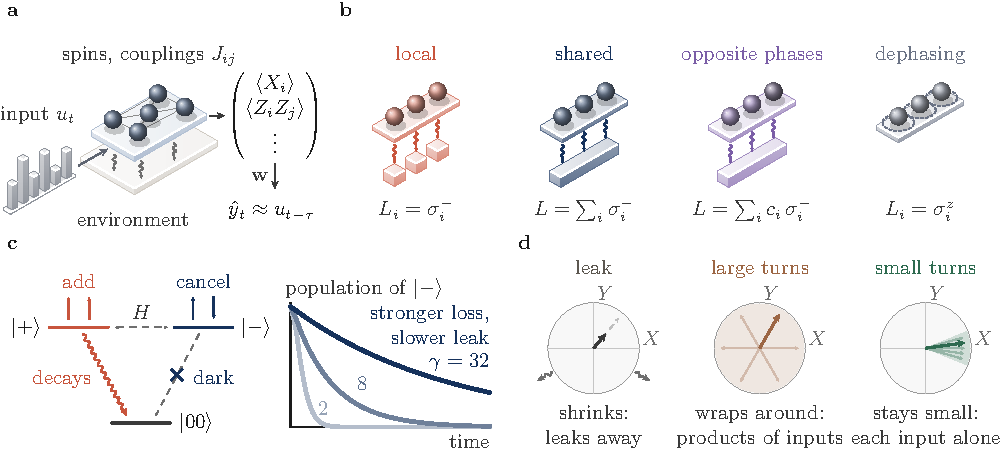
\includegraphics[width=\textwidth]{figures/fig1_concept.pdf}
\caption{\textbf{Engineering the jump operators of a quantum reservoir.}
\textbf{a}~Inputs drive interacting spins coupled to an environment; a linear readout recalls past inputs.
\textbf{b}~Jump families at equal total coupling $\Tr\sum_kL_k^\dagger L_k$, with the number of operators each leaves
untouched (protected) at five spins.
\textbf{c}~Two spins sharing one channel. The decay amplitudes of $|10\rangle$ and $|01\rangle$ add for
$|{+}\rangle$, which decays, and cancel for $|{-}\rangle$, which is dark. The Hamiltonian $H$ mixes the two; strong
loss turns this into a slow leak, so the dark state survives longer the stronger the loss (inset: coupling $g$
between $|{+}\rangle$ and $|{-}\rangle$, $\gamma/g=2$, 8, 32).
\textbf{d}~Each input turns the stored state by $\pm\theta$, so over the memory time its direction spreads by about
$\theta\sqrt{t_{\mathrm{mem}}}$. Small turns keep the spread small and the readout sees each input on its own; large
turns let it wrap around and the readout sees only products of inputs.}
\label{fig:concept}
\end{figure*}

\section{Results}

\subsection{Jump families at equal coupling}
We use the driven spin reservoir of Ref.~\cite{Sannia2024}. In step $t$ an input $u_t\in[0,1]$, drawn
independently, is held for a time $\Delta t=1/2$ while $N=5$ spins evolve under
\begin{equation}
  H(u)=\sum_{i<j}J_{ij}X_iX_j+h\sum_iZ_i+h(1+u)\sum_iX_i ,
  \label{eq:H}
\end{equation}
with $h=1/2$ and couplings $J_{ij}$ drawn uniformly from $[-1,1]$; the transverse field thus runs from $h$ to
$2h$. The environment adds a Lindblad
dissipator~\cite{Gorini1976,Lindblad1976},
\begin{equation}
  \dot\rho=-i[H(u),\rho]+\sum_k\Bigl(L_k\rho L_k^\dagger-\tfrac12\{L_k^\dagger L_k,\rho\}\Bigr).
  \label{eq:lindblad}
\end{equation}
We compare the jump families of Fig.~\ref{fig:concept}b: local loss $L_i=\sqrt\gamma\,\sigma_i^-$; one shared
channel $L=\sqrt\gamma\sum_ic_i\sigma_i^-$ with equal phases $c_i=1$ or mixed phases $c=(1,1,1,-1,-1)$; two
shared channels on three and two spins; pairwise loss $\sigma_i^-\sigma_j^-$; local loss with exchange
$\sigma_i^-\sigma_j^+$, which carry 40\% and 60\% of the coupling; local loss and gain with rates in the ratio
$1:0.3$; and local dephasing $\sigma_i^z$. Any positive mixture in the exchange and gain/loss families leaves a
single stationary state, so the weights do not decide whether stronger loss erases memory. Every family has the same total
coupling $\Tr K=80\gamma$, where $K=\sum_kL_k^\dagger L_k$ (Methods). This fixes one thing exactly: averaged over
all modes of the reservoir, the decay rate is $\Tr K/2^N$ for every family and every Hamiltonian. What differs is
how the rates are distributed.

The decisive difference is what the environment cannot reach. For local loss only the ground state is left
alone. A shared channel annihilates a whole subspace of dark states, $\binom{N}{\lfloor N/2\rfloor}$ of them on $N$
spins. With five spins it has ten, and the dissipator leaves all 100 operators on them unchanged. Pairwise loss and the split channel leave six dark
states, exchange and gain/loss a single stationary state, and dephasing leaves the 32 populations of the spin
basis but erases every coherence (Fig.~\ref{fig:concept}b).

A linear readout of the 45 single-spin and same-axis two-spin Pauli expectations reconstructs each past input.
Its recall $C_\tau\in[0,1]$ is the squared correlation between the estimate and the input $\tau$ steps back on
held-out data, and the memory $\sum_\tau C_\tau$ sums it over delays up to 300. All expectation values are
exact; there is no shot noise.

\begin{figure*}[t]
\centering
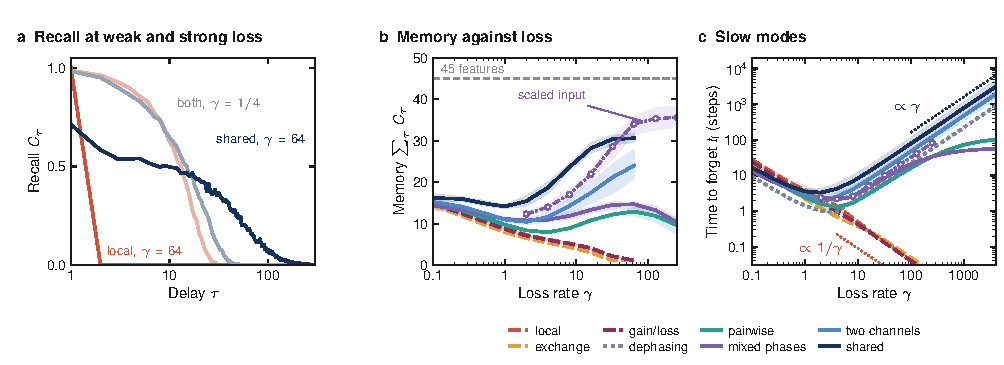
\includegraphics[width=\textwidth]{figures/fig2_families.pdf}
\caption{\textbf{The jump operators decide whether stronger dissipation erases or protects memory.}
Five-spin reservoirs at equal total coupling; lines and shading are the mean and the 16th--84th percentiles
over eight reservoirs.
\textbf{a}~Recall $C_\tau$ of the input $\tau$ steps back, for local loss and one shared channel at weak
($\gamma=1/4$, light) and strong ($\gamma=64$, dark) loss; mean over eight reservoirs.
\textbf{b}~Memory $\sum_\tau C_\tau$ for all jump families at a fixed input amplitude; one and two shared channels are
shown up to $\gamma=64$, beyond which their recall outgrows the 300 delays summed (Methods), mixed phases and pairwise
loss up to $\gamma=256$. Dash-dotted with circles, up to $\gamma=256$: mixed phases with the input amplitude scaled as
$\min(1,\gamma^{-1/2})$. Dashed: the limit of 45 set by the 45 features.
\textbf{c}~Time to forget, from the decay rates of the slow modes of the input-averaged step. Without protected
operators it falls as $1/\gamma$. With dark states it grows in proportion to $\gamma$ when the input cannot reach them
directly; with mixed phases and pairwise loss it levels off, unless the input amplitude is scaled down
(dash-dotted, mixed phases).
Dephasing protects populations into which the input never writes, so its memory in \textbf{b} is zero.}
\label{fig:families}
\end{figure*}

\subsection{Stronger dissipation, opposite consequences}
Figure~\ref{fig:families} shows the result. At weak dissipation all families behave alike, as the equal
coupling suggests (Fig.~\ref{fig:families}a,b). As $\gamma$ grows they split. With local loss, recall
retreats to ever shorter delays, until at $\gamma=64$ only the last input is left (Fig.~\ref{fig:families}a), and the
memory falls steadily (Fig.~\ref{fig:families}b). With a shared channel the memory dips and then, beyond
$\gamma\approx1$, doubles; at $\gamma=64$ recall reaches back more than a hundred steps. Exchange and gain/loss follow
local loss, and the split channel follows the shared one. Pairwise loss and mixed phases recover after a dip, but
only to their weak-dissipation level, and at stronger loss their memory falls again; we explain this difference
below.

The time to forget makes the split precise (Fig.~\ref{fig:families}c). We compute it from the slow modes of
the input-averaged step, the modes that the loss alone leaves untouched. Without protected operators it
falls as $1/\gamma$. With dark states it grows with $\gamma$. It keeps growing in proportion to $\gamma$ when the
input cannot reach the dark states directly (one shared channel, two channels); for one shared channel, $\gamma$
times the mean slow decay rate approaches about 3. When it can (mixed phases, pairwise loss), the input itself
scrambles the dark states, and the time to forget levels off, for pairwise loss only at larger $\gamma$ (Methods). Stronger loss slows forgetting only when the jump
operators leave dark states.

Dephasing shows what protection alone does not provide. Its 32 protected populations also forget ever more
slowly, yet its memory is zero at every $\gamma$: dephasing and the unitary input both leave the maximally mixed
state unchanged, and it is the unique stationary state for every input, so the reservoir relaxes to it whatever
the input. Protection is useful only for what the input can write into it. With exact features, recall counts
what is linearly recoverable however small the signal; we return to the size of the signal below.

\subsection{Dark states hold the memory}
Why does more loss help a shared channel? A strong channel acts like a continuous measurement of whether an
excitation has left, and such a measurement holds the state where the answer is
no~\cite{Beige2000,FacchiPascazio2002} (Fig.~\ref{fig:concept}c). To leading order in $1/\gamma$ the reservoir follows its Hamiltonian
projected onto the operators that the dissipator leaves alone, which turns the state but cannot forget.
Forgetting enters one order later, when the Hamiltonian briefly lifts a dark state into a bright one that
decays~\cite{Zanardi2014,Reiter2012}:
\begin{equation}
  \mathcal G(u)=\mathcal P\mathcal H(u)\mathcal P-\frac1\gamma\,\mathcal P\mathcal H(u)\mathcal S\mathcal H(u)\mathcal P ,
  \label{eq:reduced}
\end{equation}
with $\mathcal H=-i[H,\cdot\,]$, $\mathcal P$ the projector onto the protected operators and $\mathcal S$ the
inverse of the unit-rate dissipator on the rest (Methods). This is a rotation plus a leak of order $1/\gamma$:
an orthogonal map at the edge of stability, the classic recipe for long memory in a network~\cite{White2004}.
Equation~\eqref{eq:reduced} holds for any number of spins, so the leak falls as $1/\gamma$ at every size; the size
sets only its coefficient (Methods) and how strong the loss must be for this regime to begin.

Figure~\ref{fig:dark}a counts the protected operators of every family, and three tests confirm the picture.
At strong loss, 99 eigenvalues of the averaged step
approach the unit circle, one for each operator on the dark subspace apart from the stationary state; with
local loss they stay near zero (Fig.~\ref{fig:dark}b). The ten-state model of Eq.~\eqref{eq:reduced}, with
nothing fitted, reproduces the recall of the full reservoir from $\gamma\approx4$ on, within a few percent
(Fig.~\ref{fig:dark}c). Erasing the dark coordinates after every step removes all memory beyond a few
steps, while erasing a rotated copy of the same dimension leaves most of it (Fig.~\ref{fig:dark}d).

\begin{figure*}[t]
\centering
\includegraphics[width=\textwidth]{figures/fig3_dark.pdf}
\caption{\textbf{Dark states hold the memory.}
\textbf{a}~Number of operators that each unit-rate dissipator leaves unchanged, at five spins (open circle:
populations only).
\textbf{b}~Eigenvalues of the input-averaged step of one reservoir: one shared channel at $\gamma=1$, 8 and 64
(light to dark) and local loss at $\gamma=8$.
\textbf{c}~Recall of the full reservoir (lines) and of the dark-state model of Eq.~\eqref{eq:reduced} (circles),
with nothing fitted; mean of eight reservoirs.
\textbf{d}~Recall at $\gamma=16$ when the dark coordinates, or a copy of the dark subspace rotated by random
single-spin unitaries, are erased after every step; mean and 16th--84th percentiles over eight reservoirs.}
\label{fig:dark}
\end{figure*}

\subsection{The price of protection}
A long memory is not automatically a useful one. Every input turns the stored state a little, and the turn
depends on the input (Fig.~\ref{fig:concept}d). Over its memory time the stored direction thus takes a random
walk of steps $\pm\theta$ and spreads by about $\theta\sqrt{t_{\mathrm{mem}}}$. While the spread is small, the
measured projection is linear in each input. Once it reaches about a radian, the projection wraps around: the
record of an old input survives only multiplied by the inputs that followed it. A linear readout of a few
observables recovers single inputs; it cannot turn such products back into them. We call the number of distinct
inputs that a stored function involves its order, and we resolve the memory by
order~\cite{Dambre2012,MartinezPenaIPC2023} (Methods).

The simplest protected reservoir is reset to a fixed state with a small probability $p$ in each step and is
otherwise turned by an input-dependent unitary. The variance of a stored signal then decays over
$t_{\mathrm{mem}}=1/(2p)$ steps.
Write the step in traceless coordinates as an orthogonal map $O(u)$ and call $s=1-\|\mathbb EO\|_F^2/n$ the mixing
fraction of one input. It is the mean squared fraction of a randomly oriented state that one input moves away from
the average turn, and it grows as the square of the input amplitude for small turns.

\begin{theorem}[Mixing law]\label{thm:law}
Let a reservoir be reset with probability $p$ per step and otherwise turned by input-dependent rotations that
mix the stored state and write a signal (conditions in Appendix~\ref{app:law}). Draw the order $D_p$ of a stored
function with probability equal to its share of the memory. As $p\to0$, $pD_p$ becomes exponentially distributed,
with mean
\begin{equation*}
  \mathbb ED_p=s\,t_{\mathrm{mem}}+O(1).
\end{equation*}
\end{theorem}

In words, a memory mixes on average $s\,t_{\mathrm{mem}}$ inputs, the mixing fraction times the memory time.
Halving the reset probability doubles the typical order, and any fixed set of orders carries a vanishing share
of the memory although its total stays constant (Appendix~\ref{app:law}). In a protected reservoir the leakage
plays the role of $p$, so a fixed input amplitude makes memory mix more and more inputs as the loss grows.

Mixing is not only a cost. Products of inputs are the nonlinear memory that tasks such as parity
need~\cite{Dambre2012,Inubushi2017}, and the mixing law says how many inputs a reservoir combines. In the first version of
this study the equal-phase shared channel scored below local loss on parity and closed-loop
forecasting~\cite{BaumannV1} (Appendix~\ref{app:v1}). This is consistent with its input having no matrix element
between its dark states (Sec.~\ref{sec:writing}): at $\gamma=1$ its readout recovers half as much capacity of polynomial
degree three and four as that of local loss, while with mixed phases, where the input reaches the dark states
directly, it recovers as much as with local loss (Methods).

\subsection{How strongly to write}
\label{sec:writing}
Mixing is not the only cost of a large input amplitude. A single qubit that relaxes towards $+X$ at rate $\epsilon$, is
turned about $Z$ by $\pm\theta$ per input and is read along $Y$ shows the whole trade-off in closed form
(Fig.~\ref{fig:writing}a, Appendix~\ref{app:qubit}). Everything depends on $\theta^2/\epsilon$, the squared turn per
memory time. For large values the inputs mix, and they also scramble the polarization that each new input tilts,
so the stored signal shrinks. For small values each input writes too little. The stored signal is largest at
$\theta^2/\epsilon=2/\sqrt3$. Both results follow one rule: keep the mixing fraction times the memory time of order
one. With $s\propto\theta^2$ and $t_{\mathrm{mem}}\propto1/\epsilon$ this means $\theta^2\propto\epsilon$: the input
amplitude must fall as the square root of the leakage.

\begin{figure}[!tb]
\centering
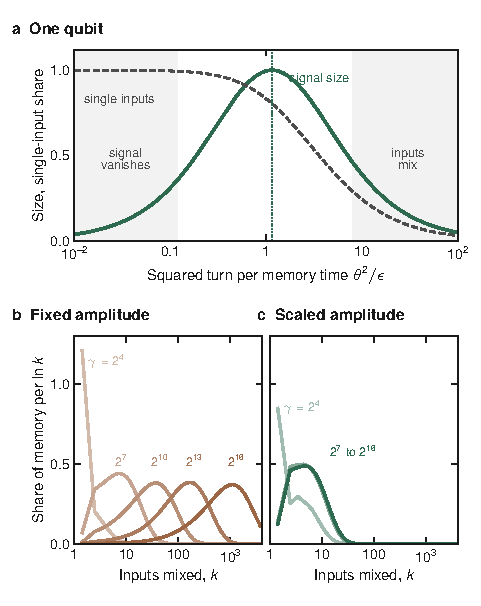
\includegraphics[width=\columnwidth]{figures/fig4_writing.pdf}
\caption{\textbf{How strongly to write into a protected reservoir.}
\textbf{a}~One qubit relaxing at rate $\epsilon$ and turned by $\pm\theta$ per input, in the limit $\epsilon\to0$ at
fixed $\theta^2/\epsilon$: size of the stored signal (normalized to its maximum at $\theta^2/\epsilon=2/\sqrt3$, dotted)
and share of single past inputs (dashed).
\textbf{b,c}~Three-spin reservoir with one shared channel of mixed phases (Hamiltonian H3): share of the memory of
$X_1$ carried by products of $k$ inputs, per unit $\ln k$, at $\gamma=2^4$, $2^7$, $2^{10}$, $2^{13}$ and $2^{16}$ (light
to dark), for a fixed input amplitude (b) and for an amplitude scaled as $8/\sqrt\gamma$ (c).}
\label{fig:writing}
\end{figure}

The jump operators decide how strongly an input reaches the protected space. The dark states of a shared
channel $L\propto\sum_ic_i\sigma_i^-$ are annihilated by $\sum_ic_i\sigma_i^-$. An input field $\sum_ic_iX_i$ along
the same phase vector is the sum of this operator and its adjoint, so it has no matrix element between dark
states. It writes only through brief excursions into bright states, and its effect falls as $1/\gamma$, while an
input pattern across the phase vector reaches the dark states directly (Methods). This explains the families of
Fig.~\ref{fig:families}. The uniform input of Eq.~\eqref{eq:H} lies along the phases of the equal-phase channel and
of each split channel, so it reaches the dark states only through bright states: their memory grows with the loss,
but the signal behind it shrinks.
For mixed phases and for pairwise loss the same input reaches the dark states directly. Their records are mixed
by later inputs, so the memory of single inputs stays near its weak-dissipation level and falls at the strongest
loss. Scaling the input amplitude
down as $\gamma^{-1/2}$ removes this limit (dash-dotted in Fig.~\ref{fig:families}b,c): with mixed phases the memory
then grows with the loss like that of the shared channel, the time to forget grows in proportion to $\gamma$ again,
and at strong loss the signal in each feature keeps a roughly constant size (Methods). The memory cannot exceed 45, one unit per feature.
It levels off near 36, and as the time to forget keeps growing each delay is recalled more weakly: the memory becomes
longer, not larger.

A three-spin reservoir with one shared channel of mixed phases, whose protected space the input reaches
directly, shows both limits (Methods). With a fixed input amplitude the order of its memory grows in proportion to
$\gamma$ and single inputs lose their share (Fig.~\ref{fig:writing}b), while the signal in a measured spin shrinks as
$1/\gamma$. With the amplitude scaled as $8/\sqrt\gamma$, which exceeds the fixed amplitude below $\gamma=64$ and
falls below it above, the order stays small (Fig.~\ref{fig:writing}c), single inputs keep a finite share, the
signal stays finite, and the range of delays that holds 90\% of the single-input recall grows in proportion to
$\gamma$. Here a single observable holds at most one unit of memory, so as the range grows each delay is recalled
more weakly, roughly as $1/\gamma$. We prove both limits for four Hamiltonians and
for neighbourhoods of their couplings with computer-assisted bounds (Appendix~\ref{app:spins}).

Which part of the protected state carries this memory? Coherence is known to shape the performance of spin
reservoirs~\cite{Palacios2024}; here we isolate its role. We return the spins to the dark subspace after every
input and compare two arms that differ only in a dephasing of the dark energy levels. The populations follow the
same slow dynamics in both arms, but without coherence the stored signal collapses as $1/\gamma^2$ (Methods). A new
input first turns a population into a coherence, and erasing the coherences deletes each record as soon as it is
written (Appendix~\ref{app:spins}).

\section{Discussion}
\label{sec:discussion}
The shape of the dissipation matters as much as its rate, and three design rules follow for the reservoirs we
studied:
\begin{enumerate}[label=(\arabic*),leftmargin=*,itemsep=2pt,topsep=4pt]
\item let the jump operators set the direction of the clock: separate channels slow it with weaker loss, a shared
  channel with dark states slows it with stronger loss, and its phases decide whether the input reaches the dark
  states;
\item let the input follow the clock, weakening it as the memory grows so that the mixing fraction of one input times
  the memory time stays of order one;
\item as a heuristic, forget by cooling, not by randomizing: prefer dissipation that leaves a polarized state the
  input can tilt.
\end{enumerate}
A damping sweet spot found at a fixed input scaling~\cite{Sannia2024} is therefore not a property of the dissipation
alone: it moves as the input weakens, and with finite sampling the measurement budget sets it. The right shape need
not be exotic: with a uniform input, weak local loss keeps the most memory at every budget we tried.

Dark states pay when the reservoir must dissipate strongly, as in waveguides, where collective decay comes with the
coupling~\cite{Zanner2022,Sheremet2023} and the positions of the spins set the phases of the channel: spins half a
wavelength apart couple with opposite signs~\cite{Sheremet2023}. Ordinary noise limits their reach: local loss or
dephasing at a small rate adds to the leak out of the dark states, which the collective loss suppresses only as
$1/\gamma$, so a memory of $T$ steps needs collective loss about $4T^2$ times stronger than local loss
(Appendix~\ref{app:numerics}). A dark state of four transmons in a waveguide lives more than a hundred times longer
than a single qubit decaying into the guide~\cite{Zanner2022}; read as such a ratio of rates, this allows a memory of
about five steps, and the fifty steps of Fig.~\ref{fig:clock}b would need a ratio near $10^4$.

Parts of this story have classical cousins: two oscillators sharing one damper keep an undamped mode, and the
$1/\gamma$ leak is the slow mode of an overdamped oscillator. The quantum structure adds three things: the protected
set is a space of operators, 100 of them for ten dark states; the memory is written into coherences between dark
energy levels; and the phases of the jump operators and the input decide whether the input reaches the protected
states at all.

Our results hold for one class of Hamiltonians, eight reservoirs and a uniform input, whose symmetry decides which
channels write gently by themselves; with the input on a single spin the collapses persist
(Appendix~\ref{app:numerics}). We study memory and capacities, which set what a linear readout can
reproduce~\cite{Dambre2012}, not a particular task. Jumps beside a transverse drive assume a bath spectrum that is
flat over the relevant frequencies~\cite{Cattaneo2019}; an open superconducting waveguide provides one up to
$\gamma\approx64$ for couplings of order a megahertz~\cite{Sheremet2023}, and shared resonators, waveguides and
structured couplers can build such channels~\cite{Cattaneo2019,Brehm2021,Sheremet2023,CattaneoPRX2023}. Concurrent
work finds that decoherence-free modes break the echo-state property and that responses below the regularization
scale do not count~\cite{Cao2026}; our dark states leak, and Sec.~\ref{sec:price} shows the second effect. Another
finds a balance between memory and nonlinearity across reservoir protocols~\cite{Cindrak2026}, which the mixing law
makes quantitative for slow memories. Truncated replay~\cite{Cindrak2024} or weak measurements~\cite{Mujal2023}
would cut the cost of sampling; how a slow clock combines with non-Markovian memory~\cite{Sannia2026Memory} is
open.

How a quantum system leaks decides not only how fast it forgets, but what it keeps and in what form.


\acknowledgments{The authors thank the Quantum Applications and Research Laboratory and the Mobile and
Distributed Systems Group at Ludwig-Maximilians-Universit\"at M\"unchen for institutional support.}

\Needspace{6\baselineskip}
\section*{Data availability}
The code, the data behind every figure and the interval certificates of the three-spin limits are available at
\url{https://github.com/eybmits/stronger-dissipation-longer-memory}; the certificates are also attached to this PDF.

\Needspace{6\baselineskip}
\section*{Author contributions}
M.B. contributed to conception, methodology, software, analysis, visualization and writing. I.F. and J.W.
contributed to methodology, interpretation and editing. C.L.-P. and J.S. contributed to supervision and
conceptual development. OpenAI Codex assisted with drafting, literature checks, derivations, code, numerical
experiments, figures and verification software; it also wrote the independent finite-rate implementation of
Appendix~\ref{app:spins} as a separate program that shares no routine with the certificate programs. All
AI-assisted material was independently reviewed and verified by the authors, who take full responsibility for the
scientific content and final manuscript.

\section{Methods}

\subsection{Five-spin simulations}
Each reservoir draws its couplings and its input stream from one seed, and every family uses the same eight
seeds. Equation~\eqref{eq:lindblad} is integrated in the 1024-dimensional basis of Pauli operators. The input is
constant within a step, and the step map $E(u)=e^{\Delta t\mathcal L(u)}$ is evaluated by Chebyshev interpolation
in $u$ at ten nodes. After a washout of $\max(800,60\gamma)$ steps we record the 45 features for 2000 training,
400 validation and 1600 test inputs. The readout is a least-squares fit with an intercept on the training and
validation inputs, and $C_\tau$ is the squared correlation of its estimate with $u_{t-\tau}$ on the test inputs.
All features are exact expectation values. Runs at $\gamma=128$ and 256 use the same seeds. There the recall of
one and two shared channels at a fixed amplitude reaches past the 300 delays we sum over (the time to forget of the
shared channel is about 200 steps at $\gamma=256$), so Fig.~\ref{fig:families}b shows them up to $\gamma=64$. The recall of
mixed phases and pairwise loss ends well within the window, and their memory falls to about 10 at $\gamma=256$. Capacities by
polynomial degree follow Ref.~\cite{Dambre2012}: products of Legendre polynomials in the past inputs $2u-1$, up to
total degree four within finite delay windows, fitted by the same features and kept above a shuffled-input noise
floor. At $\gamma=1$ degrees three and four carry 8.2 units with one shared channel, 15.9 with mixed phases and 16.4
with local loss.

For the scaled input we replace $h(1+u)$ in Eq.~\eqref{eq:H} by $h[\tfrac32+\eta(u-\tfrac12)]$ with
$\eta=\min(1,\gamma^{-1/2})$, which keeps the mean field and scales the input amplitude. With mixed phases the
variance of a feature over the test inputs, averaged over the 45 features, then stays near $5\times10^{-6}$ from
$\gamma=16$ to 256, and from $\gamma=32$ on the largest is about $2\times10^{-5}$. Meanwhile the recall of the last
input falls from 0.95 at $\gamma=64$ to 0.57 at $\gamma=256$ and spreads to longer delays; beyond delay 300 it would
add about 1\% of the memory on average. With $\eta=\min(1,2\gamma^{-1/2})$ the features vary
3.5 times more, and the memory is smaller, 29 instead of 34 at $\gamma=64$, consistent with stronger mixing. At a fixed amplitude the mean feature
variance of the equal-phase shared channel falls from $2\times10^{-4}$ at $\gamma=1$ to $4\times10^{-7}$ at $\gamma=64$
and $3\times10^{-8}$ at $\gamma=256$, while that of mixed phases stays near $8\times10^{-5}$ from $\gamma=16$ on.

\subsection{Jump families and equal coupling}
Table~\ref{tab:families} lists the jump operators. Their weights give every family the same total coupling
$\Tr K=\sum_k\Tr L_k^\dagger L_k=N2^{N-1}\gamma=80\gamma$; the mixtures for exchange and gain/loss follow the first
version of this study. For a traceless jump the superoperator trace of the dissipator is
$\Tr\mathcal D[L]=|\Tr L|^2-2^N\Tr L^\dagger L=-2^N\Tr L^\dagger L$, while the commutator with any Hamiltonian is
traceless. The $4^N$ eigenvalues $\lambda$ of the generator therefore obey
\begin{equation}
  \frac{1}{4^N}\sum\operatorname{Re}\lambda=-\frac{\Tr K}{2^N}
\end{equation}
for every family and every Hamiltonian. The protected operators form the kernel of the unit-rate dissipator,
which we compute numerically (Fig.~\ref{fig:dark}a).

\begin{table}[b]
\caption{\label{tab:families}Jump families at $N=5$, each with $\Tr K=80\gamma$, and the number of operators
that the dissipator leaves unchanged; $i<j$ for pairwise loss, $i\neq j$ for exchange and $c=(1,1,1,-1,-1)$.}
\centering\footnotesize\setlength{\tabcolsep}{4pt}
\begin{tabular}{lll}
\toprule
family & jump operators & protected\\\midrule
local & $\sqrt\gamma\,\sigma_i^-$ & 1\\
shared & $\sqrt\gamma\sum_i\sigma_i^-$ & 100\\
mixed phases & $\sqrt\gamma\sum_ic_i\sigma_i^-$ & 100\\
two channels & $\sqrt\gamma\sum_{i\le3}\sigma_i^-$, $\sqrt\gamma\sum_{i>3}\sigma_i^-$ & 36\\
pairwise & $\sqrt\gamma\,\sigma_i^-\sigma_j^-$ & 36\\
exchange & $\sqrt{0.4\gamma}\,\sigma_i^-$, $\sqrt{0.3\gamma}\,\sigma_i^-\sigma_j^+$ & 1\\
gain/loss & $\sqrt{\gamma/1.3}\,\sigma_i^-$, $\sqrt{0.3\gamma/1.3}\,\sigma_i^+$ & 1\\
dephasing & $\sqrt{\gamma/2}\,\sigma_i^z$ & 32\\
\bottomrule
\end{tabular}

\end{table}

\subsection{Slow modes}
The input-averaged step $\bar E=\mathbb E_uE(u)$ is computed by six-point Gauss--Legendre quadrature. Its
eigenvalues $\lambda_j$ give decay rates $\kappa_j=-\ln|\lambda_j|/\Delta t$. If the dissipator protects $n$
operators, the slow modes are the $n-1$ slowest decaying ones besides the stationary state, and the time to
forget is $t_{\mathrm f}=1/(\Delta t\,\bar\kappa)$ with $\bar\kappa$ their mean rate. Without protected operators we
use the slowest mode. For one shared channel $\gamma\bar\kappa=a=2.945$ to four digits from $\gamma=512$ to
16384, so $t_{\mathrm f}$ grows fourfold from $\gamma=4096$ to 16384, while it changes from 56 to 58 steps with mixed
phases and from 103 to 114 with pairwise loss. The same second-order calculation as in Eq.~\eqref{eq:reduced}, which
gives $a=2.945$ at five spins, gives $a=1.4$, 2.1 and 3.4 at three, four and six spins (mean over the same eight
coupling seeds), so the leak coefficient grows only slowly with the size. Adding local loss
$\sqrt{\gamma_{\mathrm{loc}}}\,\sigma_i^-$ gives $\bar\kappa=a/\gamma+b\gamma_{\mathrm{loc}}$. To first order in
$\gamma_{\mathrm{loc}}$, $b$ is the trace of the added dissipator on the 99 slow dark modes divided by 99,
$b=140/99\approx1.414$. Local dephasing
$\sqrt{\gamma_\phi}\,\sigma_i^z$ (the dephasing family of Table~\ref{tab:families} has $\gamma_\phi=\gamma/2$) adds
$b_\phi\gamma_\phi$ in the same way, with $b_\phi=403.2/99\approx4.073$ to first order.
For $\gamma$ from 32 to 256 and noise rates from 0.001 to 0.1 the full spectra reproduce both coefficients to within
0.2\%. A time to forget of at least $T$ steps needs $a/\gamma+b\gamma_{\mathrm{loc}}\le1/(\Delta t\,T)$, which is
possible only if $\gamma/\gamma_{\mathrm{loc}}\ge4ab\,\Delta t^2T^2\approx4.2\,T^2$; for dephasing the bound is
$4ab_\phi\Delta t^2T^2\approx12\,T^2$.

\subsection{Dark-state model and erasure}
Let $\mathcal D$ be the unit-rate dissipator, $\mathcal P=\lim_{t\to\infty}e^{t\mathcal D}$ the projector onto its
kernel and $\mathcal S=(\mathcal D+\mathcal P)^{-1}-\mathcal P$ the inverse on the decaying operators. Write
$\mathcal P=RR^\flat$ with $R^\flat R=1$, where $R$ embeds the 100 dark coordinates $\alpha$. Eliminating the
decaying operators to second order gives Eq.~\eqref{eq:reduced} for $\alpha$, and the full state is
$(R-\mathcal S\mathcal H(u)R/\gamma)\,\alpha$, which we feed to the same readout. Nothing is fitted. For the erasure
test we replace the dark coordinates after every step by their time average, $r\mapsto r-RR^\flat(r-\bar r)$; the
control erases the dark subspace rotated by a random product of single-spin unitaries. Recall is then measured at
delays 1 to 100 with 800 training, 200 validation and 800 test inputs. The write per input is
$2\|R^\flat[E(\tfrac34)-E(\tfrac14)]r_*\|$ at the stationary state $r_*$ of the equal-phase channel, for the
input patterns $(1,\dots,1)$ and $\sqrt2\cos(2\pi i/5)$ multiplying $X_i$. Along the phases it falls as $1/\gamma$,
to 0.003 at $\gamma=128$; across them it stays of order one, 0.18 at $\gamma=128$.

\subsection{Order of a memory}
For independent signs $u_t=\pm1$ the products $\prod_{j\in J}u_{t-j}$ over finite sets $J$ of delays are
orthonormal and complete; their order is $|J|$. For continuous inputs one uses orthogonal polynomials in each
input, and any centred function of one input has order one. Quantum channels act affinely on traceless
coordinates~\cite{MartinezPenaOrtega2023,MartinezPenaOrtega2025}, $r_t=A(u_t)r_{t-1}+b(u_t)$. Let $\bar A=\mathbb EA$,
$m$ the stationary mean and $\xi=A(u)m+b(u)-m$ the innovation, with covariance $V$. With
$\mathcal BX=\bar AX\bar A^{\mathsf T}$, $\mathcal TX=\mathbb E[AXA^{\mathsf T}]$ and $\mathcal K=\mathcal T-\mathcal B$, the
covariance $G_k$ carried by products of order $k$ obeys
\begin{equation}
  G_1=(1-\mathcal B)^{-1}V,\qquad G_{k+1}=(1-\mathcal B)^{-1}\mathcal KG_k ,
  \label{eq:recursion}
\end{equation}
because the mean step moves a stored product without adding a time, the fluctuating step multiplies it by the
current input, and the innovation adds the current input alone. The $G_k$ add up to the stationary covariance
$\Sigma$. A readout of features $y=Mx$ explains the share $C_k=\Tr[(M\Sigma M^{\mathsf T})^+MG_kM^{\mathsf T}]$ of
order $k$, and these shares add up to the rank of the readout~\cite{Dambre2012}. For one observable $a$,
$C_k=a^{\mathsf T}G_ka/a^{\mathsf T}\Sigma a$, and the share of single past inputs is
$a^{\mathsf T}\bar AG_1\bar A^{\mathsf T}a/a^{\mathsf T}\Sigma a$.

\subsection{Three-spin computations}
The three spins evolve under
\begin{equation}
  H_\eta(u)=\sum_{i<j}J_{ij}X_iX_j+\tfrac12\sum_iZ_i+\tfrac{3+\eta u}{4}\sum_iX_i
  \label{eq:H3}
\end{equation}
with one jump $\sqrt\gamma\,(\sigma_1^--\sigma_2^--\sigma_3^-)$, steps of $\Delta t=1/2$ and signs $u=\pm1$, at
$\eta=1$ (fixed amplitude) or $\eta=8/\sqrt\gamma$ (scaled amplitude). The dark subspace has three states. The couplings of the four
Hamiltonians H1--H4 are drawn from fixed seeds. For each loss rate we exponentiate the full generator for both
signs, solve the stationary moment equations and evaluate Eq.~\eqref{eq:recursion} for $X_1$ until 99.99\% of its
memory is accounted for; there is no sampling. The range $\tau_{90}$ is the smallest delay beyond which less than a
tenth of the recall remains. For the coherence test we apply the loss-only projector $\mathcal P$ after every
step; one arm keeps the recovered state, the other also dephases it in the energy basis of the projected
Hamiltonian. From $\gamma=2^8$ to $2^{18}$ the variance of $X_1$ stays between $10^{-4}$ and $2\times10^{-3}$ when the
coherences are kept and falls as $\gamma^{-2}$, by six orders of magnitude, when they are erased; at a fixed input
amplitude it falls as $1/\gamma$.


\appendix
\section{The mixing law}
\label{app:law}
\subsection{Precise statement}
On $n$ traceless coordinates let the step be $r_t=(1-p)O(u_t)r_{t-1}+pb$, where independent, identically
distributed inputs select orthogonal maps $O(u)$ and $b$ represents the reset state. Assume that the mean map
$A=\mathbb EO$ has spectral radius below one, that the only symmetric matrices fixed by
$X\mapsto\mathbb E[OXO^{\mathsf T}]$ are multiples of the identity, and that the input writes a signal,
$\mathbb E\|(O-A)(1-A)^{-1}b\|^2>0$. For a fixed linear readout of positive rank, draw the order $D_p$ with
probability equal to its share of the ideal memory. Then $pD_p\to\mathrm{Exp}(2/s)$ in distribution with
$s=1-\|A\|_F^2/n$, and $\mathbb ED_p=s/(2p)+O(1)$.

\emph{Idea.} One input writes a variance of order $p^2$. A covariance shape that survives for $1/(2p)$ steps
collects it to order $p$. We identify that shape and then count, with the recursion of
Eq.~\eqref{eq:recursion}, how many inputs it contains.

\subsection{Generating function}
\label{app:gen}
The order transfer $\mathcal F=(1-\mathcal B)^{-1}\mathcal K$ is a positive map on covariance matrices, and
$(1-\mathcal F)^{-1}=(1-\mathcal T)^{-1}(1-\mathcal B)=1+(1-\mathcal T)^{-1}\mathcal K$ is positive, so its spectral
radius is below one. Summing Eq.~\eqref{eq:recursion},
\begin{equation}
\begin{aligned}
  \sum_{k\ge1}z^kG_k&=z(1-z\mathcal F)^{-1}G_1,\\
  \sum_{k\ge1}kG_k&=(1-\mathcal F)^{-1}\Sigma ,
\end{aligned}
  \label{eq:generating}
\end{equation}
and $\mathcal F^K\Sigma$ is the covariance above order $K$.

\subsection{The surviving covariance}
\label{app:cov}
Let $r=1-p$, $A=\mathbb EO$, $\mathcal B_0X=AXA^{\mathsf T}$ and $\mathcal T_0X=\mathbb E[OXO^{\mathsf T}]$. Every step
contracts differences by $r$, so there is a unique stationary state. Its mean is $m_p=p(1-rA)^{-1}b=p\mu+O(p^2)$
with $\mu=(1-A)^{-1}b$, and the innovation $\xi_p=r(O-A)m_p$ has covariance $V_p=p^2V_0+O(p^3)$ with
$v=\Tr V_0=\|\mu\|^2-\|A\mu\|^2>0$ by the writing assumption. On symmetric matrices $\mathcal T_0$ preserves the trace
and the identity and contracts the Frobenius norm; by assumption the identity is its only fixed point, and power
boundedness excludes a Jordan block. Its spectral projector is $X\mapsto1\,\Tr X/n$, and all other directions have
a bounded resolvent near one. Hence
\begin{equation}
  \Sigma_p=(1-r^2\mathcal T_0)^{-1}V_p=\frac{pv}{2n}\,1+O(p^2).
  \label{eq:slowcov}
\end{equation}
The mean map is mixing, so $(1-r^2\mathcal B_0)^{-1}$ stays bounded and every fixed order has $G_k=O(p^2)$. Since
$\Sigma_y^+=O(p^{-1})$ on its support, any fixed set of orders carries a share $O(p)$, while the shares add up to the
rank $q$ of the readout.

\subsection{The number of inputs}
\label{app:inputs}
At $p=0$ the transfer $\mathcal F_0=(1-\mathcal B_0)^{-1}(\mathcal T_0-\mathcal B_0)$ fixes the identity; it is
positive and power bounded, and its unit eigenvalue is simple. Its left eigenfunctional is
\begin{equation}
  \ell(X)=\Tr[(1-A^{\mathsf T}A)X],\quad \ell(1)=ns>0,
\end{equation}
because $\ell=\Tr\circ(1-\mathcal B_0)$ and $\Tr\circ\mathcal T_0=\Tr$. Differentiating
$(1-r^2\mathcal B_0)\mathcal F_p=r^2(\mathcal T_0-\mathcal B_0)$ at $p=0$ gives $(1-\mathcal B_0)\mathcal F_0'1=-2\cdot1$,
so the leading eigenvalue is $1-\beta p+O(p^2)$ with $\beta=2n/\ell(1)=2/s$. Insert $z=e^{-\lambda p}$ into
Eq.~\eqref{eq:generating}: for fixed $\lambda\ge0$ only this eigenvalue gives a divergent resolvent term, and with
$\ell(G_1)=p^2v+O(p^3)$,
\begin{equation}
  \sum_{k\ge1}e^{-\lambda pk}G_k=\frac{pv}{\ell(1)(\lambda+\beta)}\,1+O(p^2).
\end{equation}
Divided by Eq.~\eqref{eq:slowcov} this is the Laplace transform $\beta/(\lambda+\beta)$ of the exponential law.
The second identity in Eq.~\eqref{eq:generating} gives the order-weighted covariance $\Sigma_p/(\beta p)+O(p)$, hence
$\mathbb ED_p=1/(\beta p)+O(1)=s\,t_{\mathrm{mem}}+O(1)$.

\subsection{The mixing fraction}
For a unit vector $x$ drawn uniformly, $\mathbb E\|(O-A)x\|^2=\Tr\mathcal K_0(1)/n=s$: one input moves a fraction $s$ of
a stored signal away from the average turn, and this fraction is passed to the next order. For
$O=e^{u\theta G}$ with $u=\pm1$ and skew-symmetric $G$ with eigenvalues $i\lambda_j$, the mean map is $\cosh\theta G$
and $s=n^{-1}\sum_j\sin^2\theta\lambda_j$, which grows as $\theta^2$.

\subsection{Two sectors, two laws}
The assumption of a single fixed covariance matters. Let a classical flag select one of two qubit rotations about
$Z$, by $\pm\pi/6$ or $\pm\pi/3$, and let the reset state be block diagonal. Each sector obeys the law separately,
and a single $Y$ readout sees the mixture $\Pr(pD_p>x)\to\frac12e^{-8x}+\frac12e^{-8x/3}$.

\subsection{Physical channels}
\label{app:physical}
A physical channel does not reset to a prescribed state, but the argument above only needs a single slow
covariance direction. We state the general version that Appendix~\ref{app:spins} uses and prove it along the same
four steps.

\emph{Setting.} Work on invariant reachable coordinates and translate a common limiting fixed point to zero; for the
spin reservoir of Appendix~\ref{app:spins} these are the dark coordinates, which the bright part follows at order
$\epsilon$ [Eq.~\eqref{eq:slowstep}]. The step
is $r_t=A_{u_t}(\epsilon)r_{t-1}+b_{u_t}(\epsilon)$ with a small leakage $\epsilon$, and we write $\bar A_\epsilon=\mathbb E A_u(\epsilon)$,
$\mathcal B_\epsilon X=\bar A_\epsilon X\bar A_\epsilon^{\mathsf T}$, $\mathcal T_\epsilon X=\mathbb E[A_uXA_u^{\mathsf T}]$ and
$\mathcal K_\epsilon=\mathcal T_\epsilon-\mathcal B_\epsilon$. Assume:
(i) $A_u(\epsilon)=A_{u,0}+\epsilon A_{u,1}+O(\epsilon^2)$ and $b_u(\epsilon)=\epsilon b_{u,1}+O(\epsilon^2)$ in mean square;
(ii) the mean step is mixing at $\epsilon=0$, that is, $\bar A_0$ has spectral radius below one;
(iii) the channel is mean-square stable for small $\epsilon>0$;
(iv) $\mathcal T_\epsilon$ has a simple eigenvalue $1-\kappa\epsilon+O(\epsilon^2)$ with $\kappa>0$, all its other eigenvalues stay
a fixed distance away from one, and at $\epsilon=0$ the eigenvalue has right eigenmatrix $R\succeq0$ and a left
eigenfunctional $\ell$ of $\mathcal T_0$ that is nonnegative on positive matrices, with $\ell(R)=1$;
(v) the input writes along it, $\ell(V_*)>0$, where $V_*$ is defined in step 1.

\emph{Step 1: the innovation.} The stationary mean solves $m=\bar A_\epsilon m+\mathbb Eb_u(\epsilon)$. By (ii) it is
$m_\epsilon=\epsilon m_1+O(\epsilon^2)$ with $m_1=(1-\bar A_0)^{-1}\mathbb Eb_{u,1}$. The innovation is therefore
$\xi_u=\epsilon z_u+O(\epsilon^2)$ with $z_u=A_{u,0}m_1+b_{u,1}-m_1$, and its covariance is $V_\epsilon=\epsilon^2V_*+O(\epsilon^3)$ with
$V_*=\mathbb E[z_uz_u^{\mathsf T}]$; this is the order-$p^2$ writing of Appendix~\ref{app:cov}.

\emph{Step 2: the surviving covariance.} Let $\mathcal P_\epsilon$ be the spectral projector of the simple eigenvalue in (iv);
it depends smoothly on $\epsilon$ and $\mathcal P_0X=R\,\ell(X)$. On the complement $(1-\mathcal T_\epsilon)^{-1}$ stays bounded,
while on the slow direction it divides by $\kappa\epsilon+O(\epsilon^2)$. Since $\mathcal P_\epsilon V_\epsilon=\epsilon^2\ell(V_*)R+O(\epsilon^3)$,
\begin{equation}
\begin{aligned}
  \Sigma_\epsilon&=(1-\mathcal T_\epsilon)^{-1}V_\epsilon=\epsilon\,C_*+O(\epsilon^2),\\
  C_*&=\frac{\ell(V_*)}{\kappa}\,R .
\end{aligned}
\end{equation}

\emph{Step 3: every fixed order is small.} By (ii) the spectral radius of $\mathcal B_\epsilon$ stays below one, so
$(1-\mathcal B_\epsilon)^{-1}$ is bounded. Equation~\eqref{eq:recursion} then gives $G_1=O(\epsilon^2)$ and, since $\mathcal K_\epsilon$ is
bounded, $G_k=O(\epsilon^2)$ for every fixed $k$. Its share of the observed variance of a readout $M$ tends to zero
whenever $\Tr(MC_*M^{\mathsf T})>0$. For the ideal memory of a readout with several features we also need $MC_*M^{\mathsf T}$
to have full rank on the measured support, so that $(M\Sigma_\epsilon M^{\mathsf T})^+=O(\epsilon^{-1})$; for a single observable
this holds trivially.

\emph{Step 4: the number of inputs.} At $\epsilon=0$ the order transfer $\mathcal F_0=(1-\mathcal B_0)^{-1}\mathcal K_0$ has the same
fixed points as $\mathcal T_0$, because $\mathcal F_0X=X$ is equivalent to $(1-\mathcal B_0)X=\mathcal T_0X-\mathcal B_0X$. Its left fixed
functional is $\ell_F=\ell\circ(1-\mathcal B_0)$, since $\ell_F(\mathcal F_0X)=\ell(\mathcal K_0X)=\ell(X)-\ell(\mathcal B_0X)$. Define
\begin{equation}
  s=\ell_F(R)=\ell(\mathcal K_0R).
\end{equation}
Because $\mathcal K_0X=\mathbb E[(A_{u,0}-\bar A_0)X(A_{u,0}-\bar A_0)^{\mathsf T}]$, the matrix $\mathcal K_0R$ is positive and
$s=1-\ell(\mathcal B_0R)$ lies between 0 and 1; for the same reason $\ell(\mathcal B_0Y)\le\ell(\mathcal T_0Y)=\ell(Y)$ for every
$Y\succeq0$. If $s$ vanished, then $0\le\ell(\mathcal B_0^j\mathcal K_0R)\le s=0$ for every $j$, and the Neumann series
$\mathcal F_0=\sum_{j\ge0}\mathcal B_0^j\mathcal K_0$ would give $\ell(\mathcal F_0R)=0$, which contradicts $\mathcal F_0R=R$ and
$\ell(R)=1$. So $s>0$. The fixed space of $\mathcal F_0$ is spanned by $R$, and because $\ell_F(R)=s\neq0$ the eigenvalue one
has no Jordan chain, so it is simple. Differentiating $(1-\mathcal B_\epsilon)\mathcal F_\epsilon=\mathcal T_\epsilon-\mathcal B_\epsilon$ at $\epsilon=0$ and applying it to $R$
gives $(1-\mathcal B_0)\mathcal F_0'R=\mathcal T_0'R$, hence $\ell_F(\mathcal F_0'R)=\ell(\mathcal T_0'R)=-\kappa$. First-order
perturbation of the simple eigenvalue then gives the order eigenvalue
\begin{equation}
  \mu_\epsilon=1-\beta\epsilon+O(\epsilon^2),\qquad \beta=\frac{\kappa}{s}.
\end{equation}
Insert $z=e^{-\lambda\epsilon}$ into Eq.~\eqref{eq:generating}. The other eigenvalues of $\mathcal F_0$ have modulus at most
one, because by (iii) and the positivity argument of Appendix~\ref{app:gen} the spectral radius of $\mathcal F_\epsilon$ is
below one for $\epsilon>0$, and by the simplicity shown above they differ from one, so only $\mu_\epsilon$ gives a divergent
resolvent term. Since $G_1=(1-\mathcal B_\epsilon)^{-1}V_\epsilon$ and $\ell_F$ is taken at $\epsilon=0$,
$\ell_F(G_1)=\ell(V_\epsilon)+O(\epsilon^3)=\epsilon^2\ell(V_*)+O(\epsilon^3)$, and
\begin{equation}
\begin{aligned}
  \sum_{k\ge1}e^{-\lambda\epsilon k}G_k&=\frac{\epsilon\,\ell(V_*)}{s(\lambda+\beta)}\,R+O(\epsilon^2)\\
  &=\epsilon\,C_*\,\frac{\beta}{\lambda+\beta}+O(\epsilon^2).
\end{aligned}
\end{equation}
Divided by $\Sigma_\epsilon$ from step 2 this is the Laplace transform of $\mathrm{Exp}(\beta)$, for the share of observed
variance and, under the rank condition of step 3, for the ideal memory. The second identity in
Eq.~\eqref{eq:generating} gives $\mathbb ED_\epsilon=1/(\beta\epsilon)+O(1)=s/(\kappa\epsilon)+O(1)$: $s$ is the mixing
fraction of the channel and $1/(\kappa\epsilon)$ its memory time. For the reset model, $\mathcal T_p=(1-p)^2\mathcal T_0$ gives
$\kappa=2$, $R=1$ and $\ell=\Tr/n$, so $s=1-\|A\|_F^2/n$ and $\beta=2/s$ as in Appendix~\ref{app:inputs}.

\subsection{Numerical check}
Figure~\ref{fig:law} compares the law with exact moments. For each dimension $d=2,3,4$ we draw two families of three
Haar unitaries applied with probabilities $(0.2,0.3,0.5)$, each with two reset states (a basis state and a random pure
state) and two readouts (all coordinates or one random direction). Up to $K=\lceil6/(\beta p)\rceil$ we evaluate the
remaining share $\Tr[\Sigma_y^+M\mathcal F^K(\Sigma)M^{\mathsf T}]/q$. Over these 24 reservoirs and readouts the rates lie
between 2.89 and 4.00, and the largest deviation from $e^{-\beta pK}$ falls from 0.082 at $p=0.03$ to 0.0034 at
$p=0.001$; Fig.~\ref{fig:law} shows one of them.

\begin{figure}[t]
\centering
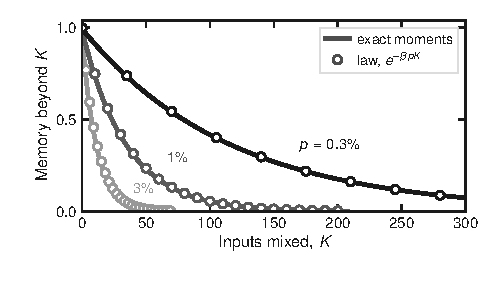
\includegraphics[width=\columnwidth]{figures/fig5_law.pdf}
\caption{\textbf{The mixing law.} Share of the ideal memory carried by products of more than $K$ inputs, for one
qubit reservoir with a reset to a basis state and a scalar readout, at reset probabilities $p=3\%$, 1\% and 0.3\%
(light to dark). Lines: exact moments; circles: the law $e^{-\beta pK}$ with $\beta=2/s=2.89$.}
\label{fig:law}
\end{figure}

\section{One qubit in closed form}
\label{app:qubit}
During one unit of time the qubit evolves under $u\theta Z/2$ and the jump $\sqrt\epsilon\,|{+x}\rangle\langle{-x}|$,
with signs $u=\pm1$, and is read along $Y$. In the Bloch plane, $\dot x=-\epsilon(x-1)-u\theta y$ and
$\dot y=u\theta x-\epsilon y/2$. For $u=+1$ write the step as
\begin{equation}
  e^{B}=\begin{pmatrix}a&-b\\ b&d\end{pmatrix},\qquad B=\begin{pmatrix}-\epsilon&-\theta\\ \theta&-\epsilon/2\end{pmatrix},
\end{equation}
with offset $(f,g)=\int_0^1e^{tB}(\epsilon,0)\,dt$; the opposite sign reverses $b$ and $g$. The stationary mean is
$(m,0)$ with $m=f/(1-a)$, and each input writes $u\,(0,v)$ with $v=bm+g$, along the measured axis.

The mean step is diagonal, while adding an input interchanges the two axes, so $Y$ carries only odd orders. By
Eq.~\eqref{eq:recursion} the variance passes from $y$ to $x$ with factor $b^2/(1-a^2)$ and back with $b^2/(1-d^2)$.
With $\chi$ their product,
\begin{equation}
\begin{aligned}
  C_{2j+1}&=(1-\chi)\chi^j, &\qquad \mathbb ED&=\frac{1+\chi}{1-\chi},\\
  \mathrm{Var}\,Y&=\frac{v^2}{(1-d^2)(1-\chi)},
\end{aligned}
\end{equation}
and the share of single past inputs is $d^2(1-\chi)$.
At fixed $\theta$ with $\sin\theta\neq0$, $1-\chi=3\epsilon/\sin^2\theta+O(\epsilon^2)$, so
$\epsilon D\to\mathrm{Exp}\bigl(3/(2\sin^2\theta)\bigr)$ and the share of single inputs vanishes even for exact
expectation values. If instead $\theta^2/\epsilon\to\nu>0$, then $a=1-(1+\nu/2)\epsilon$, $d=1-(1+\nu)\epsilon/2$ to first
order, $b\sim\theta$, $f\sim\epsilon$ and
\begin{equation}
  \chi\to\frac{\nu^2}{(\nu+2)(\nu+1)},\quad \mathrm{Var}\,Y\to\frac{4\nu}{(\nu+2)(3\nu+2)} .
\end{equation}
The mean order stays finite, the share of single past inputs tends to $1-\chi$, and since the recall beyond delay
$\tau$ is the fraction $d^{2\tau}$, the range obeys $\epsilon\tau_{90}\to\ln10/(1+\nu)$. The variance peaks at
$\nu=2/\sqrt3$. For
$\theta^2\gg\epsilon$ it vanishes as $4\epsilon/(3\theta^2)$ and for $\theta^2\ll\epsilon$ as $\theta^2/\epsilon$, so among power
laws for the angle only $\theta\propto\sqrt\epsilon$ keeps a finite signal. Density-matrix propagation reproduces these
expressions to relative error below $10^{-12}$ at 25 parameter pairs.

\section{The three-spin reservoir at strong loss}
\label{app:spins}
\emph{Idea.} At strong loss one step of the full master equation is, up to corrections of order $\epsilon=1/\gamma$, a
rotation of the dark subspace. With a fixed amplitude the two signs rotate differently; a single slow covariance
builds up, and the physical-channel version of the mixing law applies. With a scaled amplitude both signs give nearly
the same
rotation; the signal is written on the scale of the leakage and accumulates in six slow directions, which we follow
explicitly. Both arguments end in finitely many strict inequalities, which we enclose in interval arithmetic.

\subsection{What is proven}
For the four Hamiltonians of Table~\ref{tab:spins} and every Hamiltonian whose three couplings lie within $1/32$ of
theirs: with $\eta=1$, the order of the $X_1$ memory divided by $\gamma$ becomes exponentially distributed with a rate
$\beta_{\mathrm{spin}}$, and the variance of $X_1$ falls as $1/\gamma$. For the same four Hamiltonians and couplings
within $1/512$: with $\eta=8/\sqrt\gamma$, the recall of single past inputs from $X_1$ tends to a positive constant, and
its range divided by $\gamma$ tends to a positive constant.

\begin{table}[t]
\caption{\label{tab:spins}Strong-loss limits for $X_1$ in the four three-spin reservoirs: rate of the order
distribution at $\eta=1$ (certified); share of single past inputs and range at $\eta=8/\sqrt\gamma$, evaluated at
$\gamma=2^{16}$.}
\centering\footnotesize
\begin{tabular}{lccc}
\toprule
 & $\beta_{\mathrm{spin}}$ & single-input share & range$/\gamma$\\\midrule
H1 & 78.6 & 0.81 & 0.50\\
H2 & 91.7 & 0.29 & 0.18\\
H3 & 61.4 & 0.08 & 0.24\\
H4 & 132.5 & 0.14 & 0.50\\
\bottomrule
\end{tabular}

\end{table}

\subsection{The slow part of a step}
Let $\mathcal D$ be the dissipator at unit loss. Its dark space is spanned by the vacuum and the
single-excitation states with coefficients $(0,1,-1)/\sqrt2$ and $(2,1,1)/\sqrt6$; the jump is injective on two and
three excitations, so the kernel of $\mathcal D$ consists of the nine operators on the dark qutrit and all other
eigenvalues have negative real part. With $R$ embedding a Hermitian dark basis, $R^\flat=R^{\mathsf T}(\mathcal D+RR^{\mathsf T})^{-1}$,
$\mathcal P=RR^\flat$ and $\mathcal S=(\mathcal D+\mathcal P)^{-1}-\mathcal P$, perturbing the zero block of
$\mathcal D+\epsilon\mathcal H_u$ gives
\begin{equation}
  e^{\Delta t(\mathcal D/\epsilon+\mathcal H_u)}=RE_uR^\flat+\epsilon Z_u+O(\epsilon^2),
  \label{eq:slowstep}
\end{equation}
with $E_u=e^{\Delta t\,R^\flat\mathcal H_uR}$,
where $Z_u$ contains the two boundary terms $-\mathcal S\mathcal H_uRE_uR^\flat$ and $-RE_uR^\flat\mathcal H_u\mathcal S$ and the
leak $-\Delta t\,R^\flat\mathcal H_u\mathcal S\mathcal H_uR$ inside the exponential.

\subsection{Fixed amplitude}
At $\eta=1$ the dark rotations $O_u$ of the two signs differ. Two finite tests show that their mean is mixing and that
the identity is the only fixed dark covariance: $\|\bar O^{4096}\|_F<0.013$, and $1-T_D+vv^{\mathsf T}$ is invertible,
where $T_DX=\mathbb E[O_uXO_u^{\mathsf T}]$ and $v=1/\sqrt8$. The first-order terms of Eq.~\eqref{eq:slowstep} give the
writing strength $w$, the decay rate $\kappa$ of the slow covariance and the mixing fraction
$s_0=1-\|\bar O\|_F^2/8$, all certified positive. The physical-channel version of the mixing law then gives
$\beta_{\mathrm{spin}}=\kappa/s_0$, and the variance of $X_1$ is $\tfrac43(w/\kappa)\epsilon+O(\epsilon^2)$ because $X_1$
has overlap $1/6$ with the slow covariance. Throughout the boxes of half-width $1/32$, a coupling change $r$ moves each
dark rotation by at most $3r$, and ball arithmetic keeps $w$, $\kappa$ and $s_0$ above 0.0001, 3.53 and 0.052.

\subsection{Scaled amplitude}
At $\eta=g\sqrt\epsilon$, $g=8$, both signs give the same leading rotation $E$. A block exponential of the static,
drive and leak generators gives the mean step $E+\epsilon E_1$ and the fluctuating part $u\sqrt\epsilon D_1$. The six
coherence phases of the static dark Hamiltonian are separated from one another and from one, so the unit-eigenvalue
space of $E$ contains only populations, on which $E_1$ generates a population dynamics with a unique stationary state
$m_*$. The inputs therefore write $\pm\sqrt\epsilon\,v$ with $v=D_1m_*$, which lies in the coherence planes. The fixed
covariances of the rotation form a six-dimensional space: three population covariances and one identity per coherence
plane. On it the first-order generators
\begin{equation}
\begin{aligned}
  K_BX&=\mathcal P_6(E_1'XO^{\mathsf T}+OXE_1'^{\mathsf T}),\\
  K_TX&=K_BX+\mathcal P_6(D_1'XD_1'^{\mathsf T})
\end{aligned}
\end{equation}
are certified stable, and the summed linear response and the full covariance converge to $W_*=-K_B^{-1}\mathcal P_6(vv^{\mathsf T})$
and $\Sigma_*=-K_T^{-1}\mathcal P_6(vv^{\mathsf T})$. The recall of single inputs from $X_1$ tends to
$a^{\mathsf T}W_*a/a^{\mathsf T}\Sigma_*a$, and after $t/\epsilon$ steps the remaining fraction is
$a^{\mathsf T}e^{tK_B}W_*a/a^{\mathsf T}W_*a$, which crosses $0.1$ once; this crossing is the range divided by $\gamma$.
Interval tests bracket it to $4\times10^{-6}$. The certificates show $a^{\mathsf T}W_*a>0$, and since
$\Sigma_*\succeq W_*$ the limiting share is positive; the archived certificates state this numerator bound through the
recall of a readout with 1000 shots, which has the same numerator. On the boxes of half-width $1/512$, Sturm counts
and Weyl's bound keep the six phases separated and $-(K+K^{\mathsf T})$ positive definite for both generators, so the
limits stay positive.

The single-input shares in Table~\ref{tab:spins} range from 0.08 to 0.81 because the limit compares two rates of the
same order in $\epsilon$: $K_B$, at which the mean step lets a stored signal decay, and the extra term of $K_T$, at
which the random signs of later inputs turn it into products. Their ratio depends on the couplings through the dark
energies and the matrix elements of $X_1$ between dark states, so the mean order in the limit runs from 1.4 for H1 to
5.9 for H3. The boxes are 16 times narrower than for the fixed amplitude because this argument follows the dark
energy eigenstates themselves: a coupling change $r$ moves each eigenprojector by up to $3r/(\delta-3r)$, where $\delta$ is the
smallest gap between dark energies, whereas the fixed-amplitude argument needs only the rotations, which move by at
most $3r$.

\subsection{Erasing coherence}
Returning bright population to the dark subspace after every step leaves the leading terms of the scaled step
unchanged, so it keeps the same limits. Dephasing in the dark energy basis removes the coherence planes into which
$v$ writes. Restricted to populations, the two signs then differ only at order $\epsilon^{3/2}$, because the
order-$\sqrt\epsilon$ response of a diagonal state is off-diagonal, while the populations still follow $1+\epsilon L$.
A new input therefore writes a vector of size $\epsilon^{3/2}$, the slow dynamics accumulate its square over
$1/\epsilon$ steps, and the stored signal is $O(\epsilon^2)$.

\subsection{Certificates}
The attached archive \texttt{spin\_certificates.zip} contains the generators, the exact couplings and the interval
programs. At 192-bit precision they reproduce the archived enclosures; at 256 bits they check every strict inequality
above. An independent implementation (see Author contributions) that builds the full finite-rate maps and
extrapolates to infinite loss agrees
with the certified rates to $2\times10^{-7}$ and with the limiting recalls to $4\times10^{-9}$.

\section{Results of the first version}
\label{app:v1}
Table~\ref{tab:v1} repeats the benchmark comparison of the first version~\cite{BaumannV1} at $\gamma=1$, where the
same jump families have the same total coupling. The shared channel had the largest memory and the smallest NARMA-10
error but scored below local loss on parity and on closed-loop Mackey--Glass forecasting, two tasks that need products
of past inputs; at this operating point it also led local loss in memory and NARMA-10 error from four to eight spins.
Figure~\ref{fig:v1} repeats its finite-sampling test: when the 45 features are estimated from a finite number of
preparations per step, the advantage of the shared channel over local loss becomes significant only above about
$2\times10^5$ preparations per step if all spins are read in three grouped settings, and only above about
$3\times10^6$ if every feature is measured separately.

\begin{table}[h]
\caption{\label{tab:v1}Benchmark scores of the first version~\cite{BaumannV1} at $\gamma=1$, $h=\Delta t=1/2$, five
spins and 45 features, for parity read at 15 times within each step: mean over 32, 32, 16 and 64 reservoirs, with the standard error in the last digits in
parentheses. Memory sums $C_\tau$ over delays 1 to 20 and parity sums a capacity over windows of one to seven inputs
(larger is better); NARMA-10 and Mackey--Glass forecasting (MG) over 150 closed-loop steps are normalized errors
(smaller is better). The rows are those of the six jump families studied here; bold marks the best of them.}
\centering\footnotesize\setlength{\tabcolsep}{4pt}
\begin{tabular}{lllll}
\toprule
family & memory & NARMA-10 & parity & MG\\\midrule
local & 8.63(7) & 0.315(8) & 4.82(4) & \textbf{0.037(3)}\\
shared & \textbf{12.21(10)} & \textbf{0.229(6)} & 3.78(3) & 0.097(9)\\
pairwise & 9.20(8) & 0.289(7) & 4.75(4) & 0.039(4)\\
gain/loss & 8.31(6) & 0.337(8) & 4.85(4) & 0.046(4)\\
exchange & 7.41(5) & 0.441(9) & \textbf{5.08(5)} & 0.052(4)\\
dephasing & 0 & 1.020(6) & 0 & 0.0599(4)\\
\bottomrule
\end{tabular}
\end{table}

\begin{figure}[h]
\centering
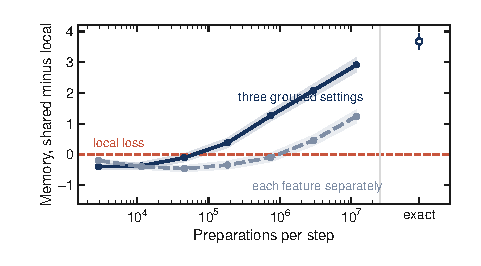
\includegraphics[width=\columnwidth]{figures/fig6_sampling.pdf}
\caption{\label{fig:v1}\textbf{Finite sampling in the first version.} Memory of one shared channel minus that of
local loss at $\gamma=1$ when every feature is estimated from a finite number of preparations per step, with all spins
read along $X$, $Y$ or $Z$ in three grouped settings (solid) or each feature measured separately (dashed). Lines and
bands show the mean and 95\% interval over 20 reservoirs; the open circle is exact. Data from
Ref.~\cite{BaumannV1}.}
\end{figure}



\begingroup
\bibliographystyle{quantum}
\bibliography{references}
\endgroup

\end{document}
